\documentclass[russian,10pt]{article}

\usepackage[intlimits]{amsmath}
\usepackage{amsthm,amsfonts}
\usepackage{amssymb}
\usepackage{mathrsfs}
%\usepackage{graphicx}
\usepackage[final]{graphicx,epsfig} 
\usepackage{longtable}
\usepackage{indentfirst}
\usepackage[utf8]{inputenc}
\usepackage[T2A]{fontenc}
\usepackage[russian,english]{babel}
\usepackage[usenames]{color}
\usepackage{esint}
\usepackage{bbm}
\usepackage{styles/mystyle}


\pdfpagewidth 14cm
\pdfpageheight 20cm

\textwidth 11cm
\textheight 16.5cm
\oddsidemargin 1.5cm % 1.84cm
\topmargin 1.5cm % 1.8cm
\footskip 1cm

\hoffset -1in
\voffset -1in
\headheight 0pt
\headsep 0pt

\hyphenpenalty=300
%\tolerance=800
\binoppenalty=10000

\clubpenalty=10000 \widowpenalty=10000  % подавление "висячих строк"
\tolerance=2000  % терпимость к жидким строкам
\righthyphenmin=2  % минимальное число символов при переносе* 

% Adjust first page number according to real document position in the book.
\setcounter{page}{1}

% Dot after section number
\makeatletter
% In section title
\def\@seccntformat#1{\csname the#1\endcsname.\quad}
\makeatother

%\tolerance = 2000

% To place author above title
\def\maketitle{
  \begin{center}


\thispagestyle{empty} 
\begin{center}

МИНИСТЕРСТВО ОБРАЗОВАНИЯ И НАУКИ \\
РОССИЙСКОЙ ФЕДЕРАЦИИ \\

 $ $ \\

Московский физико-технический институт \\
(государственный университет) \\
 
  $ $ \\ $ $ \\ $ $ \\
  $ $ \\
  $ $  \\
\smallskip
\smallskip
\premierAuthors, \\
\autresAuthors \\
 
 $ $ \\ $ $ \\
 
\textbf{СТОХАСТИЧЕСКИЙ АНАЛИЗ \\ В ЗАДАЧАХ} \\
 
 $ $ \\
  $ $ \\
  $ $ \\
Учебно-методическое пособие \\
 
  $ $ \\ $ $ \\ $ $ \\ $ $ \\
  \smallskip
   Часть 2
 $ $ \\ $ $ \\ $ $ \\ $ $ \\ $ $ \\ $ $ \\
 
Москва--Долгопрудный 2015


\end{center}

\newpage
  \end{center}
}

\renewcommand{\refname}{Литература}

%\sloppy
%\DeclareGraphicsRule{*}{eps}{*}{}
\DeclareMathOperator{\diam}{diam}

\graphicspath{{images/}}
\newcommand{\imgh}[3]{\begin{figure}[!h]\center{\includegraphics[width=#1]{#2}}\caption{#3}\label{Fig:#2}\end{figure}}

% Perfectly typesetted tilde for url links.
%\def\urltilde{\kern -.15em\lower .7ex\hbox{\~{}}\kern .04em}

\addto{\captionsrussian}{
	\renewcommand{\proofname}{\bf Решение}
}

\usepackage{wasysym}
\usepackage{verbatim}

\makeatletter
\g@addto@macro\th@definition{\thm@headpunct{.}}
\makeatother
\theoremstyle{definition}


%\newtheorem{problem}{\noindent\normalsize\bfЗадача \No\!\!}
\newtheorem{problem}{\noindent\normalsize\bf{}}[section]

\renewcommand{\theproblem}{\noindent\arabic{problem}}

\newtheorem*{example}{\noindent\normalsize\bf{}Пример}
\newtheorem*{definition}{\noindent\normalsize\bf{}Определение}
\newtheorem*{remark}{\noindent\normalsize\bf{}Замечание}
\newtheorem{theorem}{\noindent\normalsize\bf{}Теорема}
\newtheorem*{lemma}{\noindent\normalsize\bf{}Лемма}
\newtheorem*{suite}{\noindent\normalsize\bf{}Следствие}


\newtheorem*{ordre}{\noindent\normalsize\bf{}Указание}

\newenvironment{solution}{\begin{proof}\vspace{1em}} {\end{proof} \vspace{2em}}

\newcommand{\atoc}[1]{\addtocontents{toc}{\hspace{0.4\linewidth}#1\par}}

%\newcommand{\fixme}[1]{\textcolor{red}{\noindent\normalsize\frownie{}[#1]}} %for displaying red texts

\newcommand{\fixme}[1]{}


\usepackage{enumitem}

\RequirePackage{enumitem}
\renewcommand{\alph}[1]{\asbuk{#1}} % костыль для кирилической нумерации 

\setenumerate[1]{label=\alph*), fullwidth, itemindent=\parindent, 
  listparindent=\parindent} 
\setenumerate[2]{label=\arabic*), fullwidth, itemindent=\parindent, 
  listparindent=\parindent, leftmargin=\parindent}

\newcommand{\rg}{\ensuremath{\mathrm{rg}}}
\newcommand{\grad}{\ensuremath{\mathrm{grad}}}
\newcommand{\diag}{\ensuremath{\mathrm{diag}}}
\newcommand{\const}{\ensuremath{\mathop{\mathrm{const}}}\nolimits}
\newcommand{\Var}{\ensuremath{\mathop{\mathbb{D}}}\nolimits}
\newcommand{\Exp}{\ensuremath{\mathrm{{\mathbb E}}}}
\newcommand{\PR}{\ensuremath{\mathrm{{\mathbb P}}}}
\newcommand{\Be}{\ensuremath{\mathrm{Be}}}
\newcommand{\Po}{\ensuremath{\mathrm{Po}}}
\newcommand{\Beta}{\ensuremath{\mathrm{Beta}}}
\newcommand{\Dir}{\ensuremath{\mathrm{Dir}}}
\newcommand{\Bi}{\ensuremath{\mathrm{Bi}}}
\newcommand{\Ker}{\ensuremath{\mathrm{Ker}}}
\newcommand{\Real}{\ensuremath{\mathrm{Re}}}
\newcommand{\Lin}{\ensuremath{\mathrm{Lin}}}
\newcommand{\Gl}{\ensuremath{\mathrm{Gl}}}
\newcommand{\mes}{\ensuremath{\mathrm{mes}}}
\newcommand{\cov}{\ensuremath{\mathrm{cov}}}
\newcommand{\I}{\ensuremath{\mathrm{I}}}
\newcommand{\N}{\ensuremath{\mathcal{N}}}
\newcommand{\KL}{\ensuremath{\mathcal{KL}}}
\newcommand{\Star}{\hspace{-6pt}*\hspace{3pt}}
\newcommand{\DStar}{\hspace{-6pt}**\hspace{3pt}}
\newcommand{\Nbb}{\mathbb{N}}

\usepackage{watermark}
\thiswatermark{\put(-100,-550){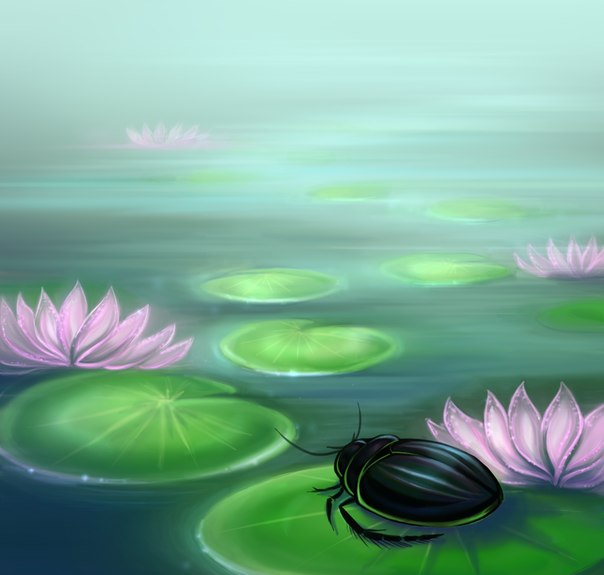
\includegraphics[scale=0.8]{images/guk.jpg}} }

\usepackage{url}
\makeatletter
\g@addto@macro{\UrlBreaks}{\UrlOrds}
\makeatother

\begin{document}

\selectlanguage{russian}

\maketitle

\atoc{Часть 1}

\thispagestyle{empty} 

УДК 519.21
 
 $ $ \\ $ $ \\
 
\premierAuthors, \autresAuthors. Стохастический анализ в задачах: Учебно-методическое пособие. Часть 1 / МФТИ. М.--Д., 2015, изд. 3-е, доп.

$ $ \\ 
 
\begin{abstract}

Содержит программу, список литературы и задачи одноименного курса, читаемого сотрудниками кафедры Математических основ управления студентам факультета управления и прикладной математики Московского физико-технического института. Задачи могут быть использованы в качестве упражнений на семинарских занятиях, сдачах заданий, экзаменах, а также при самостоятельном освоении курса. В новое издание добавлен ряд задач, отражающих также опыт преподавания вероятностных дисциплин в Независимом московском университете и опыт наших коллег из ПреМоЛаб МФТИ, преподающих вероятностные дисциплины в ведущих научных центрах Германии и Франции. Данный сборник задач разрабатывался с учетом направлений подготовки: студентов МФТИ, студентов НМУ, магистров факультета Компьютерных наук ВШЭ и магистров факультета Прикладной математики БФУ им. И.~Канта.  

 $ $ \\ $ $ \\ $ $ \\ $ $ \\ $ $ 

\noindent рецензенты: д.ф.-м.н. А.В. Колесников \\
\noindent проф. Факультета математики НИУ ВШЭ \\
\noindent д.ф.-м.н. А.Н. Соболевский \\ 
\noindent проф. Независимого московского университета, \\ зам. директора ИППИ РАН 

\end{abstract}


  
 \newpage 


\thispagestyle{empty} 
\begin{center}

{ОБЯЗАТЕЛЬНАЯ ЧАСТЬ ПРОГРАММЫ УЧЕБНОГО КУРСА  \\ 
«Теория вероятностей»  }
 
\end{center}
 
 {\small
 
Интуитивные предпосылки теории вероятностей. Множество элементарных исходов опыта, событие. Классическое и статистическое определение вероятности. Математическое определение вероятности. Алгебра и сигма-алгебра событий, минимальная сигма алгебра. Аксиомы теории вероятностей и следствия из них. Вероятностное пространство.

Теорема непрерывности вероятности. Теорема сложения вероятностей. Зависимые и независимые события. Условная вероятность события. Формула полной вероятности. Формула Байеса. Леммы Бореля--Кантелли. Закон ``0-1'' Колмогорова.

Случайная величина как измеримая функция. Функция распределения случайной величины. Дискретные и непрерывные случайные величины. Плотность распределения вероятностей. Формула включений-исключений.

Конкретные распределения случайных величин. Схема Бернулли, геометрическое и биномиальное распределение. Простейший поток событий и распределение Пуассона. Показательное, равномерное, нормальное, log-нормальное и отрицательно-биномиальное распределения. Бета-распределение и гамма-распределение.

Случайный вектор. Функция распределения случайного вектора. Зависимые и независимые случайные величины, условные законы распределения. Функции случайных величин. Невырожденное функциональное преобразование случайного вектора.
Интеграл Стилтьеса. Математическое ожидание и дисперсия случайной величины. Моменты случайной величины. Условное математическое ожидание. Корреляционная матрица случайного вектора. Коэффициент корреляции двух случайных величин.

Характеристическая функция и ее свойства. Связь моментов случайной величины с ее характеристической функцией. Разложение характеристической функции в ряд.
Сходимость последовательностей случайных величин с вероятностью единица (почти наверное), порядка $p$ (в среднем квадратичном), по вероятности, по распределению. Соотношение между различными типами сходимости. 

Неравенство Чебышева. Закон больших чисел. Критерий Колмогорова. Теоремы Хинчина и Чебышева.  Усиленный закон больших чисел. Теорема Колмогорова и Бореля. Оценивание скорости сходимости частоты к вероятности в схеме Бернулли. Неравенство Бернштейна. 

Интегральная и локальная теоремы Myавра--Лапласа. Дискретная поправка. Теорема Линдберга. Центральная предельная теорема для одинаково распределенных случайных величин. Центральная предельная теорема в форме Натана. Условие Ляпунова. Теорема Гливенко.
}


\newpage

\section{Введение}

В основу предлагаемого сборника задач по теории вероятностей положены задачи (в том числе повышенной сложности), предлагавшиеся в разные годы студентам факультета управления и прикладной математики (ФУПМ) МФТИ и Независимого московского университета на семинарах, сдачах заданий и экзаменах. Главными отличительными особенностями пособия являются: а) широкий спектр представленного материала, б) отражение ряда современных направлений развития теории вероятностей и в) нацеленность на приложения.

По замыслу авторов, предлагаемый сборник задач отчасти демонстрирует роль курса как “вероятностного фундамента” для ряда других дисциплин: прикладной статистики, стохастических дифференциальных уравнений, эффективных алгоритмов, экспериментальной экономики (финансовой математики) и др. Несмотря на широкий спектр представленных тем, основной  акцент делается на формирование у читателей геометрической интуиции, восходящей к Пуанкаре, которая позволяет с единых позиций понять многообразие асимптотических результатов стохастической теории как проявление одного общего принципа концентрации меры. 

Большое внимание в сборнике уделяется различным приемам доказательства предельных теорем – асимптотических результатов теории вероятностей. Для этого прежде всего используется аппарат производящих функций и теории функций комплексного переменного.

Более половины представленных в сборнике задач не являются стандартными. Для таких задач даны указания, комментарии (замечания), ссылки на публикации. 

Желающих более глубоко изучить представленные темы отсылаем к списку литературы, приведенному в конце сборника задач. 

Следует отметить, что за последние десять лет заметно возросло значение для выпускников Физтеха глубоких знаний вероятностных дисциплин. Это обусловлено множеством причин.

Прежде всего, это вызвано широким распространением задач анализа больших массивов данных (machine learning, data mining). Подтверждением служит взаимная востребованность студентов ФУПМ и Школы анализа данных компании Яндекс, большая популярность среди  студентов ФУПМ кафедры интеллектуальных систем (заведующий кафедрой член-корреспондент РАН К.В. Рудаков, Вычислительный центр РАН) и кафедры предсказательного моделирования (заведующий кафедрой академик РАН А.П. Кулешов, Институт проблем передачи информации РАН). 
%Во многом именно для таких студентов и написаны разделы \ref{bayes}, \ref{zb4}, \ref{MK}, \ref{stats}, ССЫЛКА[Оптимизация и стохастика]. %3 – 6, 9, 10.

Другая не менее важная причина -- разработка эффективных (приближенных, рандомизированных) алгоритмов решения сложных задач. 
%Этому посвящены разделы \ref{MK}, \ref{information}, \ref{CS}, ССЫЛКА[Оптимизация и стохастика].
Сложно, например, представить себе современного специалиста по моделированию, который бы не использовал методы Монте-Карло. Также сложно представить себе специалиста в области computer science, которому не приходилось бы применять рандомизированные алгоритмы и подвергать алгоритмы вероятностному анализу (например, для оценки сложности в среднем). 

Еще одна причина  связана с тем, что приложение вероятностных методов к анализу и разработке экономических моделей для части студентов ФУПМ является фундаментом в работе на базовых кафедрах. Например, заведующие базовыми кафедрами ФУПМ член-коррерспондент РАН И.Г. Поспелов (Вычислительный центр РАН) и  член-коррерспондент РАН Ю.С. Попков (Институт системного анализа РАН) активно работают в направлении разработки вероятностных моделей экономических агентов и вероятностного анализа агломерационных моделей. %Этому посвящен раздел ССЫЛКА[Марковские модели макросистем].

Наконец, можно заметить, что задачи анализа больших компьютерных, социальных, транспортных сетей в последнее время выходят на передний план во многих приложениях. Огромную роль в изучении таких сетей играют вероятностные модели, некоторые из которых будут приведены в предлагаемом сборнике задач. 
%Разделы \ref{hard}, \ref{genF}, \ref{combinatorics}, ССЫЛКА[Марковские модели макросистем] сборника посвящены изучению подобных сетей, в частности, различным предельным переходам.

Важную роль в подготовке настоящего сборника задач сыграла Лаборатория структурных методов анализа данных в предсказательном моделировании (ПреМоЛаб), открытая на базе ФУПМ МФТИ в 2011 году. В частности, благодаря этой лаборатории, у студентов есть возможность посмотреть на сайте www.mathnet.ru, www.premolab.ru (семинары: Стохастический анализ в задачах, Математический кружок и др.) видеозаписи выступлений ведущих ученых, посвященные ряду нестандартных задач из этого сборника. 

Мы благодарны нашим коллегам Д.В. Беломестному, Я.И.~Белопольской, М.Л.~Бланку, Н.Д.~Введенской, В.В.~Веденяпину, Д.П.~Ветрову, А.М.~Вершику, К.В.~Воронцову, В.В.~Вьюгину, В.В.~Высоцкому, А.В.~Калинкину, М.Н.~Вялому, М.С.~Гельфанду, Э.Х.~Гимади, Г.К.~Голубеву, А.Б.~Дайняку, П.Е.~Двуреченскому, Н.Х.~Ибрагимову, М.И.~Исаеву, Г.А.~Кабатянскому, А.В.~Колесникову, А.В.~Леонизову, Г.~Лугоши, Ю.В.~Максимову, В.А.~Малышеву, В.Д.~Мильману, В.В.~Моттлю, Т.А.~Нагапетяну, А.В.~Назину, Ю.Е.~Нестерову, А.С.~Немировскому, В.И.~Опойцеву, Ф.В.~Петрову, С.А.~Пирогову, Б.Т.~Поляку, И.Г.~Поспелову, А.М.~Райгородскому, В.Н.~Разжевайкину, М.А.~Раскину, В.Г.~Редько, A.Е.~Ромащенко, А.В. Савватееву, А.Н.~Соболевскому, А.~Содину, В.Г.~Спокойному, Й.~Стоянову, У.~Сэндхольму, С.П.~Тарасову, И.О.~Толстихину, М.Ю.~Хачаю, О.С.~Федько, Ю.А.~Флёрову, А.X.~Шеню, оказавшим заметное влияние на формирование различных разделов этого учебного пособия, и А.А. Шананину, во многом способствовавшему развитию на ФУПМ базового цикла вероятностных дисциплин. Также отметим большую помощь старшекурсников, аспирантов ФУПМ и участников нашего стохастичексого семинара в НМУ и Физтехе в вычитке этого сборника задач (в особенности, Д.~Бабичева, А.~Балицкого, Ф.~Гончарова, Ю.~Дорна, Е.~Клочкова, А.~Макарова, Е.~Молчанова, Н.~Животовского, М.~Панова, Л.~Прохоренкову(Остроумову), А.~Суворикову, Д.~Петрашко, М.~Широбокова).

\begin{center}
\textbf{
Список обозначений
}
\end{center}

\noindent $\langle \Omega, \mathcal{F}, \PR \rangle$ -- вероятностное пространство ($\Omega$ -- множество исходов, $\mathcal{F}$ -- $\sigma$-алгебра, $\PR$ -- вероятностная мера); \\
$p(x), \; f(x), \; f_X(x)$ -- плотность распределения случайной величины $X$;
$\Exp X$ -- математическое ожидание случайной величины $X$; \\
$\Exp_p X$ -- математическое ожидание $X$ с плотностью распределения $p$; \\
$\Exp_\PR X$ -- математическое ожидание $X$ по мере $\PR$; \\
$\Var X$ -- дисперсия случайной величины $X$; \\
$\N(m,\sigma^2)$ -- нормальное распределение; \\
$\Po(\lambda)$ -- распределение Пуассона; \\
$\Dir(\alpha_1,...,\alpha_n)$ -- распределение Дирихле;\\
$\Beta(\alpha,\beta)$ -- бета-распределение;\\
$\Be(p)$ -- распределение Бернулли; \\
$R[a,b], [a,b]$ -- равномерное распределение; \\
$\Phi(x)$ -- функция стандартного нормального распределения $\N(0,1)$; \\
$\mathrm{Exp}(x)$ -- показательное распределение; \\
$\overset{d}{\longrightarrow}$ $\left(\mathop{\longrightarrow}\limits_{n\to\infty}^{d}\right)$ -- сходимость по распределению, в ряде случаев $n\to\infty$ опущено во избежание громоздких обозначений; \\
$\overset{p}{\longrightarrow}$ -- сходимость по вероятности; \\
$\overset{\text{п.н.}}{\longrightarrow}$ -- сходимость с вероятностью 1;\\
$[x^{n}]\varphi(x)$ -- коэффициент при $x^n$ в разложении в степенной ряд функции $\varphi(x)$;\\
с.в. -- случайная величина; \\
з.б.ч. -- закон больших чисел; \\
х.ф. -- характеристическая функция; \\
ц.п.т. -- центральная предельная теорема; \\
ПФ -- производящая функция; \\
ЭПФ -- экспоненциальная производящая функция;\\
$\langle \cdot, \cdot\rangle$ -- скалярное произведение; \\
Индикаторная функция:
\[
\I(\text{true}) = [\text{true}] = 1, \quad \I(\text{false}) = [\text{false}] = 0;
\]
Простая выборка с плотностью распределения $p$:
\[
X_1,\ldots,X_n \sim p(X);
\]
В схожих ситуациях используется символ $\in$ вместо $\sim$ (например, $X \in \N(m, \sigma^2)$), если подразумевается принадлежность случайной величины  семейству распределений, $\sim$ также обозначает пропорциональность; \\ 
Ненормированная плотность распределения:
\[
p(x) \propto g(x), \quad p(x) = \frac{g(x)}{\int g(x) dx};
\]
Математическое ожидание по заданной переменной:
\[
\Exp_X h(X,Y) = \int_{-\infty}^{+\infty} h(x,Y) dF(x); 
\]
Дивергенция Кульбака--Лейблера для распределений $\PR_1$ и $\PR_2$ с общим носителем~$\Omega$ (соответствующие плотности распределений обозначены как $p_1$ и $p_2$):
\[
\KL(\PR_1 \Vert \PR_2) = \int_{\Omega} \log \left( \frac{p_1(x)}{p_2(x)} \right) p_1(x) dx;
\]
Дивергенция Кульбака--Лейблера для распределения $\PR_\theta$, зависящего от параметра (соответствующая плотность распределения обозначена как $p(x| \theta)$):
\[
\KL(\theta_1 \Vert \theta_2) = \KL(\PR_{\theta_1} \Vert \PR_{\theta_2});
\]
$A \triangle B = A \setminus B + B \setminus A$ -- симметрическая разность; \\
$\log = \ln$; \\
$\mathcal{B}$ -- борелевская сигма алгебра;






\thispagestyle{empty} 
\tableofcontents
\newpage


\section{Стандартные задачи}
\label{standart}


%\subsection{Дискретное равномерное распределение}


\begin{problem}
Некто имеет $N$ ключей, из которых только один от его двери. Какова вероятность того, что, используя ключи в случайном порядке, 
он откроет дверь 
\begin{enumerate}
\item[а)] первым ключом; 
\item[б)] последним ключом? 
\end{enumerate}
Требуется найти вероятность того, что потребуется не менее $k$ попыток, чтобы открыть дверь, если ключи, которые не подошли 
\begin{enumerate}
\item[в)] откладываются; 
\item[г)] не откладываются. 
\end{enumerate}

\begin{ordre}
В пункте в) воспользоваться заменой вероятности бинарной величины на математическое ожидание.
\end{ordre}

\end{problem}


\begin{problem}
Ребенок играет с десятью буквами разрезной азбуки: А, А, А, Е, И, К, М, М, Т, Т. 
Какова вероятность того, что при случайном расположении букв в ряд он получит слово <<МАТЕМАТИКА>>? 
\end{problem}


\begin{problem}
Казалось бы, при бросании двух игральных костей как 9, так и 10 можно получить двумя разными способами: $9 = 3+6 = 4+5$, $10 = 4+6 = 5+5$. В случае бросания трех костей 9 и 10 получаются 6 различными способами. Почему тогда 9 появляется чаще, когда бросают две кости, а 10, когда бросают три? 
\end{problem}



\begin{problem}(Парадокс раздела ставки \cite{2013}, \cite{book12})
Два игрока играют в безобидную игру (с вероятностью победы в каждой из партий 1/2). Они договорились, что тот, кто первым выиграет 6 партий, получит  весь приз. Предположим, что игроки не успели доиграть: первый выиграл 5 партий а, второй -- 3. Как следует разделить приз?   
\end{problem}

\begin{problem}(Вероятностный парадокс лжеца \cite{book2012})
Если Вы выберете ответ на этот вопрос случайно, какова вероятность правильного ответа?

а) 25{\%}; б) 50{\%}; в) 60{\%}; г) 25{\%}.
\end{problem}

\begin{problem}
Из урны, содержащей $a$ белых, $b$ черных и $c$ красных шаров, последовательно извлекаются три шара. Найдите 
вероятность следующих событий: 
\begin{enumerate}
\item[а)] все три шара разного цвета; 
\item[б)] шары извлечены в последовательности белый, черный, красный; 
\item[в)] шары извлечены в обратной последовательности. 
\end{enumerate}
\end{problem}



\begin{problem}
Из урны, содержащей $a$ белых и $b$ черных шаров, извлекается наугад один шар и откладывается в сторону. Какова вероятность 
того, что извлеченный наугад второй шар окажется белым, если: 
\begin{enumerate}
\item[а)] первый извлеченный шар белый; 
\item[б)] цвет  первого извлеченного шара остается неизвестным? 
\end{enumerate}
\end{problem}


\begin{problem}(Задача Стефана Банаха \cite{2013}, \cite{29})
В двух спичечных коробках имеется по $n$ спичек. На каждом шаге наугад выбирается коробок, и из него удаляется (используется) 
одна спичка. Найдите вероятность того, что в момент, когда один из коробков опустеет, в другом останется $k$ спичек. 
\end{problem}

\begin{ordre}
Событие, удовлетворяющее условию задачи -- из выбранного коробка взяли последнюю спичку, а в другом коробке имеется $k$ спичек. 
\end{ordre}

\begin{problem}
Партия продукции состоит из десяти изделий, среди которых два изделия дефектные. Какова вероятность того, что из пяти отобранных 
наугад и проверенных изделий: 
\begin{enumerate}
\item[а)] ровно одно изделие дефектное; 
\item[б)] ровно два изделия дефектные; 
\item[в)] хотя бы одно изделие дефектное? 
\end{enumerate} 

\begin{ordre}
В пункте в) удобнее искать вероятность противоположного события.
\end{ordre}

\end{problem}

\begin{problem}
Известно, что в результате бросания десяти игральных костей выпала  по крайней мере одна «шестерка». Какова вероятность того, что число выпавших «шестерок» больше единицы?
\end{problem}

\begin{problem}
Найти вероятность того, что из $50$ студентов, присутствующих на лекции по теории вероятностей, хотя бы двое имеют одну и ту же дату рождения. 

\begin{remark}
Для получения приближенного решения можно воспользоваться свойством линейности математического ожидания следующих событий $X_{ij}$ -- у  $i$-го и  $j$-го человека дни рождения совпадают.  
\end{remark}

\end{problem}


\begin{problem}
В урне находится $m$ шаров, из которых $m_1$ белых и $m_2$ черных $(m_1 + m_2 = m)$. 
Производится $n$ извлечений одного шара с возвращением его (после определения его цвета) обратно в урну. Найти вероятность того, 
что ровно $r$ раз из $n$ будет извлечен белый шар. 
\end{problem}


\begin{problem}
Найти вероятность того, что при размещении $n$ различных шаров по $N$ различимым ящикам заданный ящик будет содержать ровно 
$k$: $0\leqslant k\leqslant n$, шаров (все различимые размещения равновероятны). 
\end{problem}


\begin{problem}
В урне находится $m$ шаров, из которых $m_1$ --- первого цвета, $m_2$ --- второго цвета, $\ldots$, $m_s$ --- $s$-го цвета 
$(m_1+m_2+\ldots +m_s=m)$. 
Производится $n$ извлечений одного шара с возвращением его (после определения его цвета) обратно в урну. Найти вероятность того, 
что $r_1$ раз будет извлечен шар первого цвета, $r_2$ раз --- шар второго цвета, $\ldots$, $r_s$ раз --- шар $s$-го цвета 
$(r_1+r_2+\ldots +r_s=n)$. 
\end{problem}


\begin{problem}
\label{sec:clubok}
Из клубка с $n$ разноцветными веревочками выходит $2n$ концов. Свяжем их попарно в случайном порядке (все возможные варианты связок равновероятны); получится несколько (зацепленных друг за друга) веревочных колец разной длины. Найдите математическое ожидание числа колец.
\end{problem}

\begin{ordre}
Задача (взятая из \cite{book2012}) легко сводится к подсчету математического ожидания числа циклов в случайной перестановке (см. задачу \ref{permloop} из раздела \ref{genF}). 
\end{ordre}


\begin{problem}
\label{vkl_iskl}
Пусть $A_1,\ldots,A_n$ -- последовательность событий, для которой известно, что:
\[
\PR_1 = \underset{i = 1}{\overset{n}{\sum}} \PR(A_i), \;
\PR_2 = \underset{i < j}{\sum} \PR(A_i \cap A_j), \;
\PR_k = \underset{i_1 < \ldots < i_k}{\sum} \PR(A_{i_1} \cap \ldots \cap A_{i_k}).
\]

 Покажите, что для всех нечетных $k$ справедливо неравенство
 \[
 \PR(A_{i_1} \cup \ldots \cup A_{i_k}) \leq \underset{j = 1}{\overset{k}{\sum}} (-1)^{j+1}\PR_j,    
 \]
  а для всех четных $k$
 
 \[
 \PR(A_{i_1} \cup \ldots \cup A_{i_k}) \geq \underset{j = 1}{\overset{k}{\sum}} (-1)^{j+1}\PR_j.	
 \]

 
\end{problem}

\begin{remark}
При $k=n$ получим неравенство, известное как \textit{формула включений-исключений}.
\end{remark}

\begin{problem}
В гардеробе случайным образом перепутались $N$ одинаковых шляп посетителей. Какова вероятность того, что хотя бы один посетитель получит свою шляпу (рассмотреть случаи $N=4$, $N=10000$)?  
\end{problem}

\begin{ordre}
Воспользоваться формулой включений-исключений (см. задачу \ref{vkl_iskl}).
\end{ordre}

\begin{problem}
Несколько раз бросается игральная кость. Какое событие более вероятно: 
\begin{enumerate}
\item[а)] сумма выпавших очков четна; 
\item[б)] сумма выпавших очков нечетна? 
\end{enumerate}
\end{problem}


\begin{problem}
Для уменьшения общего количества игр $2n$ команд спортсменов разбиваются на две подгруппы. Определить вероятности того, что 
две наиболее сильные команды окажутся: 
\begin{enumerate}
\item[а)] в одной подгруппе; 
\item[б)] в разных подгруппах. 
\end{enumerate}
\end{problem}


\begin{problem}
В урне находятся $a$ белых и $b$ черных шаров, которые наугад по одному без возвращения извлекаются из урны до тех пор, пока урна не опустеет. 
Какое событие более вероятно: 
\begin{enumerate}
\item[а)] первый извлеченный шар белый; 
\item[б)] последний извлеченный шар белый? 
\end{enumerate}
\end{problem}



\begin{problem}
В урне находятся $a$ белых и $b$ черных шаров. Шары наугад по одному извлекаются из урны без возвращения. Найти вероятность того, 
что $k$-й вынутый шар оказался белым. 
\end{problem}


\begin{problem}
$30$ шаров размещаются по $8$ ящикам так, что для каждого шара одинаково возможно попадание в любой ящик. Найти вероятность 
размещения, при котором будет $3$ пустых ящика, $2$ ящика --- с тремя, $2$ ящика --- с шестью и $1$ ящик --- с двенадцатью шарами. 
\end{problem}


\begin{problem}
$N$ частиц случайно и независимо друг от друга размещаются в $k$ ячейках так, что каждая из них попадает 
в $i$-ую ячейку с вероятностью $p_i$ $(i=1,\ldots,k, \sum\limits_{i=1}^{k} p_i=1)$. Найти вероятность того, что число частиц в ячейках 
примет заданные значения $n_1$, $\ldots$, $n_i$, $\ldots$, $n_k$ (полиномиальное распределение). 
\end{problem}

\begin{problem}
Из $n$ лотерейных билетов $k$ --- выигрышные $(n\geqslant 2k)$. Какова вероятность, что среди $k$ купленных билетов по крайней мере 
один будет выигрышным? 
\end{problem}

\begin{comment}
\begin{problem}
Из совокупности всех подмножеств множества $\{1,2,\ldots,N\}$ по схеме выбора с возвращением выбираются множества $A$ и $B$. 
Найти вероятность, что $A$ и $B$ не пересекаются. 
\end{problem}
\end{comment}





\begin{comment}
\begin{problem}
В самолете $n$ мест. Есть $n$ пассажиров, выстроившихся друг за другом в очередь. Во главе очереди -- <<заяц>>. У всех, 
кроме <<зайца>>, есть билет, на котором указан номер посадочного места. Так как <<заяц>> входит первым, он случайным образом занимает 
некоторое место. Каждый следующий пассажир, входящий в салон самолета, действует по такому принципу: если его место свободно, то 
садится на него, если занято, то занимает с равной вероятностью любое свободное. Найдите вероятность того, что последний пассажир 
сядет на свое место. 
\end{problem}
\end{comment}


\begin{problem}(Какие автобусы переполнены? \cite{book2012}) Двое кончают работу 
одновременно и идут к автобусной остановке вместе. Каждый уезжает на первом 
подъехавшем автобусе: одному нужен 24-й автобус, другому 25-й. При этом 
первый считает, что в среднем 24-е автобусы более полные, а второй -- что 
25-е. Почему так может быть?
\end{problem}

\begin{problem}(Задача Кавалера де Мере) 
Что более вероятно: при одновременном бросании четырех игральных костей получить хотя бы одну единицу или при $24$ бросаниях 
 по две игральные кости одновременно получить хотя бы один раз две единицы? Найти вероятности указанных событий. 
\end{problem}


\begin{problem}
Из $2^N$ множеств: совокупности всех подмножеств множества $\{1,2,\ldots,N\}$ случайно и независимо выбираются 2 множества $A$ и $B$. Найти вероятность, что $A$ и $B$ не пересекаются.
\end{problem}

\begin{problem}(Н.Н. Константинов \cite{book2012})
В самолете $n$ мест. Есть $n$ пассажиров, выстроившихся друг за другом в очередь. Во главе очереди -- ``заяц''. У всех, 
кроме ``зайца'', есть билет, на котором указан номер посадочного места. Так как ``заяц'' входит первым, он случайным образом занимает 
некоторое место. Каждый следующий пассажир, входящий в салон самолета, действует по такому принципу: если его место свободно, то 
садится на него, если занято, то занимает с равной вероятностью любое свободное. Найдите вероятность того, что последний пассажир 
сядет на свое место. 
\end{problem}





%\subsection{Схема испытаний Бернулли}

\begin{problem}
Опыт состоит в подбрасывании симметричной монеты до тех пор, пока два раза подряд она не выпадет одной и той же стороной. Подбрасывания независимы в совокупности. 
Построить пространство элементарных событий и найти вероятности следующих событий: 
\begin{enumerate}
\item опыт окончится до шестого бросания; 
\item для завершения опыта потребуется четное число бросаний. 
\end{enumerate}
\end{problem}

\begin{problem}(Pаспределение Паскаля или отрицательно биномиальное распределение)
Найдите распределение дискретной случайной величины равной количеству произошедших неудач в последовательности испытаний Бернулли с вероятностью успеха $p$, проводимой до $r$-го успеха.

\end{problem}

\begin{problem}
При каждом подбрасывании монета падает вверх орлом с вероятностью $p>0$. Пусть $\pi _{n} $ -- вероятность того, что число орлов после $n\in {\mathbb N}$ независимых подбрасываний будет чётно. Показав, что $\pi _{n+1} =\left(1-p\right)\cdot \pi _{n} +p\cdot \left(1-\pi _{n} \right)$, $n\in {\mathbb N}$, или иным способом найдите~$\pi _{n} $. 
\end{problem}

\begin{comment}
\begin{problem}
Симметричную монету независимо бросили $n$ раз. Результат бросания записали в виде последовательности нулей и единиц. Покажите, что с вероятностью стремящейся к единице при $n\to \infty $ длина максимальной подпоследовательности из подряд идущих единиц лежит в промежутке
\[\left(\log \sqrt{n} ,\; \log n^{2} \right).\] 
\end{problem}
\end{comment}

\begin{problem}

В так называемой ``безобидной игре'' с повторениями участвуют два игрока. Начальный капитал первого игрока равен $z$ руб, второго~--~$\infty$. В каждой партии первый игрок выигрывает или проигрывает 1 руб с вероятностью $0.5$, независимо от предшествующих партий. Обозначим за $z + s_k$ капитал первого игрока после $k$-й итерации, $\eta(z)$ -- число шагов до разорения:
\[
\eta(z) = \min \{k: z + s_k = 0 \}.
\]     
Покажите, что с вероятностью 1 первый игрок разорится $\PR(\eta(z)<\infty) = 1$, но при этом $\Exp \eta(z) = \infty$.  

\end{problem}

\begin{ordre}
Получите рекуррентные соотношения для вероятности разорения и  $\Exp \eta(z)$. Допустив  $\Exp \eta(z) < \infty$, придите к противоречию, доказав $\Exp \eta(z) < 0$ при больших $z$.
\end{ordre}

\begin{problem}
Сколько раз в среднем нужно подбросить монету, чтобы решка выпала два раза подряд?
\end{problem}



\begin{problem} (Честная игра \cite{book2012})
Два человека играют в {\it орлянку} (кидают симметричную монету, и ставят по рублю: один на орла, другой на решку). У каждого есть своя монетка, и каждый подозревает партнера в несимметричности его монетки. Предложите правила (как имея, эти две монеты ``сгенерировать'' симметричную монету), по которым игра будет гарантированно честной?
\end{problem}

%\subsection{Независимость и условные вероятности}

\begin{problem}
Приведите пример вероятностного пространства и трёх событий на этом пространстве, которые попарно независимы, но зависимы в совокупности. Предложите обобщение полученной конструкции, в котором любые $n$ из $(n+1)$ событий независимы в совокупности, а все $(n+1)$ -- зависимы в совокупности.
\end{problem}

\begin{ordre}
См. задачу \ref{bernshtein}, \cite{book12}, \cite{stoianov}.
\end{ordre}

\begin{problem}
Показать, что из независимости событий $A$ и $B$ следует независимость событий $A$ и $\overline B$, $\overline A$ и $B$, 
$\overline A$ и $\overline B$. 
\end{problem}


\begin{problem}
Показать, что из равенства ${\mathbb P}(A\, |\, B)={\mathbb P}(A\, |\, \overline B)$ для ненулевых событий $A$ и $B$ следует 
равенство ${\mathbb P}(AB)={\mathbb P}(A){\mathbb P}(B)$, т.е. их независимость. 
\end{problem}


\begin{problem}(Пример Бернштейна, \cite{stoianov})
\label{bernshtein}
Подбрасываются три игральные кости. События $A$, $B$ и $C$ означают выпадение одинакового числа очков (соответственно) на первой и 
второй, на второй и третьей, на первой и третьей костях. Являются ли эти события независимыми 
\begin{enumerate}
\item[а)] попарно, 
\item[б)] в совокупности? 
\end{enumerate}
\end{problem}


\begin{problem}
Имеется три картонки. На одной с обеих сторон нарисована буква $A$, на другой -- $B$, а на третьей с одной стороны -- $A$, с другой -- $B$. Одна из картонок выбирается наугад и кладется на стол. Предположим, что на видимой стороне картонки оказывается буква $A$. Какова вероятность, что на второй стороне тоже $A$?  (См. \cite{2013}).
\end{problem}




\begin{problem}
Пусть $A$, $B$, $C$ --- заданные события. Доказать справедливость неравенств 
\begin{enumerate}
\item ${\mathbb P}(AB)+{\mathbb P}(AC)+{\mathbb P}(BC)\geqslant {\mathbb P}(A)+{\mathbb P}(B)+{\mathbb P}(C)-1$; 
\item ${\mathbb P}(AB)+{\mathbb P}(AC)-{\mathbb P}(BC)\leqslant {\mathbb P}(A)$; 
\item ${\mathbb P}(A\bigtriangleup B)\leqslant {\mathbb P}(A\bigtriangleup C)+{\mathbb P}(C\bigtriangleup B).$ 
\end{enumerate}
\end{problem}

\begin{problem}(Задача A.A. Натана \cite{5})
Вероятности конъюнкций событий $A$, $B$ и $C$ приведены в таблице истинности: 
\vspace{0.3cm}

\begin{tabular}{|c|c|c|c|}
\hline
$\quad A\quad$ & $\quad B\quad$ & $\quad C\quad$ & $\quad {\mathbb P}(ABC)\quad$ \\
\hline
$0$ & $0$ & $0$ & $20/36$ \\
\hline
$0$ & $0$ & $1$ & $5/36$ \\
\hline
$0$ & $1$ & $0$ & $5/36$ \\
\hline
$0$ & $1$ & $1$ & $0$ \\
\hline
$1$ & $0$ & $0$ & $5/36$ \\
\hline
$1$ & $0$ & $1$ & $0$ \\
\hline
$1$ & $1$ & $0$ & $0$ \\
\hline
$1$ & $1$ & $1$ & $1/36$ \\
\hline
\end{tabular}

\vspace{0.3cm}

Можно ли наблюдаемые события $A$ и $B$ использовать как признаки, используемые для обнаружения события $C$? 
\end{problem}

\begin{problem}
Юноша собирается сыграть три теннисных матча со своими родителями, и для победы он должен победить два раза подряд. 
Порядок матчей может быть следующим: отец--мать--отец, мать--отец--мать. Юноше нужно решить, какой порядок для него предпочтительней, 
учитывая, что отец играет лучше матери (См. \cite{book12}). 

\end{problem}


\begin{problem}
Имеются две урны. В одной из них находится один белый шар, в другой --- один черный шар (других шаров урны не содержат). Выбирается 
наугад одна урна. В нее добавляется один белый шар и после перемешивания один из шаров извлекается. Извлеченный шар оказался белым. 
Определить апостериорную вероятность того, что выбранной оказалась урна, которая первоначально содержала белый шар. 
\end{problem}


\begin{problem}
В первой урне содержится $a$ белых и $b$ черных шаров (и только они), во второй --- $c$ белых и $d$ черных шаров 
(и только они). Из выбранной наугад урны извлекается один шар, который обратно не возвращается. Извлеченный шар оказался белым. 
Найти вероятность того, что и второй шар, извлеченный из той же урны, окажется белым. 
\end{problem}

\begin{problem}(Парадокс Монти Холла \cite{book12})
Представьте, что вы стали участником игры, в которой находитесь перед тремя дверями. Ведущий поместил за одной из трех 
пронумерованных дверей автомобиль, а за двумя другими дверями --- по козе (козы тоже пронумерованы) случайным образом --– это значит, 
что все $3! = 6$ вариантов расположения автомобиля и коз за пронумерованными дверями равновероятны). У вас нет никакой информации 
о том, что за какой дверью находится. Ведущий говорит: <<Сначала вы должны выбрать одну из дверей. После этого я открою одну из 
оставшихся дверей (при этом если вы выберете дверь, за которой находится автомобиль, то я с вероятностью $1/2$ выберу дверь, 
за которой находится коза номер $1$, и с вероятностью $1-1/2=1/2$ дверь, за которой находится коза номер $2$). Затем я предложу 
вам изменить свой первоначальный выбор и выбрать оставшуюся закрытую дверь вместо той, которую вы выбрали сначала. Вы можете 
последовать моему совету и выбрать другую дверь, либо подтвердить свой первоначальный выбор. После этого я открою дверь, 
которую вы выбрали, и вы выиграете то, что находится за этой дверью.>> Вы выбираете дверь номер $3$. Ведущий открывает дверь номер $1$ 
и показывает, что за ней находится коза. Затем ведущий предлагает вам выбрать дверь номер $2$. Увеличатся ли ваши шансы 
выиграть автомобиль, если вы последуете его совету? 
\end{problem}


\begin{problem}
Известно, что $96\%$ выпускаемой продукции соответствует стандарту. Упрощенная схема контроля признает годным с вероятностью 
$0.98$ каждый стандартный экземпляр аппаратуры и с вероятностью $0.05$ -- каждый нестандартный экземпляр аппаратуры. Найти вероятность того, 
что изделие, прошедшее контроль, соответствует стандарту. 
\end{problem}


\begin{problem}
Пусть отличник правильно решает задачу с вероятностью 0.95, а двоечник с вероятностью 0.15. Сколько задач нужно дать на зачете и сколько требовать решить, чтоб отличник не сдал зачет с вероятностью не большей 0.01, а двоечник сдал зачет с вероятностью не большей 0.1?
\end{problem}


\begin{problem}(Задача про мужика)
Пусть некоторый мужик говорит правду с вероятностью 75\% и лжет с 
вероятностью 25\%. Он подбрасывает симметричную кость и говорит, 
что ``выпала 6''. C какой вероятностью выпала 6?
\end{problem}

\begin{problem}
Рассмотрим лампочку, которая может ломаться и устройство, которое чинит лампочку, мгновенно, когда та выходит из строя. При этом считается, что времена работы лампочки от поломки до поломки распределены как $\xi \in \text{Exp}(\lambda)$ и не зависят друг от друга. Чинящее устройство, в свою очередь, тоже может ломаться. Распределение времени работы этого устройства, $\eta \in \text{Exp}(\mu)$, и не зависит от времени работы лампочки. Найти распределение времени работы всей системы в целом. Рассмотреть случаи когда $\lambda = \mu$ и $\lambda \neq \mu$.
\end{problem}



\begin{problem}
В $(m+1)$ урне содержится по $m$ шаров, причем урна с номером $n$ содержит $n$ белых и $(m-n)$ черных шаров $(n = 0,1,\ldots,m)$. 
Случайным образом выбирается урна и из нее $k$ раз с возвращением извлекаются шары. Найти: 
\begin{enumerate}
\item[а)] вероятность того, что следующим также будет извлечен белый шар, при условии, что все $k$ шаров оказались белыми, 
\item[б)] ее предел при $m\to\infty$. 
\end{enumerate}
\end{problem}

\begin{ordre}
Применить \textit{формулу полной вероятности} в следующем виде 
$$
{\mathbb P}(B\, |\, A)=\sum\limits_{n=1} {\mathbb P}(B\, |\, H_n A){\mathbb P}(H_n\, |\, A).
$$
\end{ordre}


\begin{problem}
Параметр $p$ (вероятность выпадаения <<орла>>) в схеме испытаний Бернулли является равномерно распределенной случайной величиной на отрезке $[0.1, 0.9]$ и разыгрывается до начала испытаний, причем $p$ не изменяется от опыта к опыту. В серии из $n=1000$ бросаний было подсчитано число успехов $r=777$.  Найдите условную плотность распределения $p(x|r=777)$. Оцените, как изменится ответ, если известно, что точное значение числа успехов $r\in[750, 790]$.
\end{problem}


\begin{comment}
\begin{problem}
\begin{enumerate}
\item Имеется монетка (несимметричная). Несимметричность монетки заключается в том, что либо орел выпадает в два раза чаще решки; 
либо наоборот (априорно (до проведения опытов) оба варианта считаются равновероятными). Монетку бросили $10$ раз. Орел выпал $7$ раз. 
Определите апостериорную вероятность того, что орел выпадает в два раза чаще решки (апостериорная вероятность считается с учетом 
проведенных опытов (иначе говоря, это просто условная вероятность)). 

\item Определите апостериорную вероятность того, что орел выпадает не менее чем в два раза чаще решки. Если несимметричность 
монетки заключается в том, что либо орел выпадает не менее чем в два раза чаще решки; либо наоборот (априорно оба варианта считаются 
равновероятными). 
\end{enumerate}
\end{problem}
\end{comment}

\begin{problem}
Пусть $X$ и $Y$ ~--– независимые случайные величины,  имеющие распределение Пуассона. 
Доказать, что случайная величина $Z = X + Y$ имеет распределение Пуассона. 
Выявить вид условного распределения случайной величины $X$ при фиксированном значении случайной величины $Z$.
\end{problem}


%\subsection{Вероятностное пространство, $\sigma$–алгебра}

\begin{problem}
Показать, что борелевская $\sigma$-алгебра в ${\mathbb R}^1$, содержащая все числовые промежутки вида $[a,b)$, 
содержит все промежутки вида $(a,b)$, $(a,b]$, $[a,b]$ и отдельные точки прямой. 

\begin{ordre}
Учесть свойство замкнутости $\sigma$-алгебры относительно операций 
объединения, пересечения и вычитания. 
\end{ordre}

\end{problem}


\begin{problem}
Пусть $\Omega = [a,b]\times...\times[a,b]$, $\mathcal{F}$ --- $\sigma$–алгебра, содержащая все отрезки 
$[\alpha_1,\beta_1]\times...\times[\alpha_n,\beta_n]$ $(a \leqslant \alpha_1 < \beta_1 \leqslant b, \ldots, a \leqslant \alpha_n < \beta_n \leqslant b)$ с вероятностной мерой 
\[
{\mathbb P}\{ \omega_1  \in [\alpha_1,\beta_1], ..., \omega_n  \in [\alpha_n,\beta_n]  \}=\dfrac{\mes[\alpha_1, \beta_1]}{\mes[a,b]}  \ldots  \dfrac{\mes[\alpha_n, \beta_n]}{\mes[a,b]}.
\]
Показать, что 
\begin{enumerate}
\item ${\mathbb P}\{ \omega_1=c=\const\}=0$; 
\item ${\mathbb P}\{ \omega_1=\omega_2\}=0$;
\item найти вероятность ${\mathbb P}\{ \omega_1 \leq \omega_3 \leq \omega_2\}$. 
\end{enumerate}

\end{problem}


\begin{problem}
Число элементарных событий некоторого вероятностного пространства равно $n$. Указать минимальное и максимальное возможные значения 
для числа событий. 
\end{problem}

\begin{problem}
Может ли число всех событий какого-либо вероятностного пространства быть равным $129$; $130$; $128$? 
\end{problem}


\begin{problem}(Задача о встрече \cite{2})
\label{L_extension}
Два лыжника условились о встрече между $10$ и $11$ часами утра у подножья тягуна, причем договорились ждать друг друга не более $10$ минут, чтобы не замерзнуть. Считая, что момент прихода на встречу каждым выбирается ``наудачу'' в пределах указанного часа, найти вероятность того, что встреча состоится. 
\end{problem}

\begin{remark}
В подобного рода задачах, где явно не определена вероятностная тройка $\langle \Omega, \mathcal{F}, \PR \rangle$ в общем случае следует придерживаться такой последовательности действий: 
\begin{enumerate}
\item Задать вероятностную меру на множествах простой структуры;
\item Продолжить вероятностную меру на множества более сложной структуры, рассматриваемые в задаче;  
\item Проверить условия, гарантирующие $\sigma$-аддитивность продолженной меры.   
\end{enumerate}
Рассмотрим каждый из этапов в отдельности, придерживаясь контекста задачи о встрече. Возьмем $\Omega = [0,1] \times [0,1]$. В качестве множеств простой структуры $\text{П}$ удобно воспользоваться \textit{полукольцом с единицей} $\Leftrightarrow$ $C_i, A, B \in \text{П}$, $C_i \cap C_j  = \emptyset$:
\[
\Omega \in \text{П},  \quad A\cap B \in \text{П}, \quad A_{\supset B} \setminus B = \bigcup \limits_{i=1}^n C_i.
\]
Зададим меру $\PR$ на $\text{П}$, $\Omega \subseteq \mathbb{R}^n$ при помощи формулы 
\[
\PR\{ [x_1^{(0)}, x_1^{(1)})\times \ldots \times [x_n^{(0)},  x_n^{(1)})  \} = 
\]
\[\tag{1} =
\begin{cases}
\sum \limits_{\alpha_1, \ldots, \alpha_n} (-1)^{\sum \alpha_i} F\left(x_1^{(\alpha_1)} ,\ldots, x_n^{(\alpha_n)}\right),  \; n \; \text{четно}, \\
\sum \limits_{\alpha_1, \ldots, \alpha_n} (-1)^{\sum \alpha_i - 1} F\left(x_1^{(\alpha_1)} ,\ldots, x_n^{(\alpha_n)} \right) ,  \; n \; \text{нечетно},\\
\end{cases}
\]
тогда выполнимость свойств аддитивной вероятностной меры $\PR$ равносильна  выполнимости свойств (1-6) для функции $F$, а $\sigma$-аддитивность равносильна свойству 7: 

\begin{enumerate}
\item[1.] Неотрицательность;
\item[2.] Монотонность по каждой координате;
\item[3.] $F(x_1, \ldots, x_n) \to 0$ при $x_i \to -\infty$;
\item[4.] $F(x_1, \ldots, x_n) \to 1$ при $x_1, \ldots, x_n  \to \infty$;
\item[5.] $F(x_1^{(1)},...,x_n^{(1)}) - F(x_1^{(0)},...,x_n^{(0)}) \geq 0, \, x_i^{(1)}\geq x_i^{(0)}, \, i=\overline{1,n}$;
\item[6.] $F(x_1, \ldots, x_n) \to  F(x_1, \ldots x_{i-1}, x_{i+1}  \ldots , x_n)$ при $x_i \to \infty$;
\item[7.] Непрерывность слева в точках разрыва.
\end{enumerate} 

Заметим также, что если $\PR$ абсолютно непрерывна, то существует функция плотности распределения  $f(x_1 ,\ldots, x_n ) \geq 0$, что гарантирует выполнение свойств (1-7), т.е. $\PR$ является  $\sigma$–аддитивной вероятностной мерой на  $\text{П}$.
Продолжим вероятностную меру на класс множеств 
\[\mu \tilde{A} \supset \{t_1, t_2 \in \Omega: |t_1 - t_2| =\tau \}\]
посредством \textit{пополнения по Лебегу} (см. Константинов Р.В. Лекции по функциональному анализу. Долгопрудный, 2007г):
\[
\PR^{*}(B) = \inf \limits_{B \subseteq \bigcup \limits_{i=1}^{\infty} A_i} \sum \limits_{i=1}^{\infty} \PR(A_i)
\]
 \[
 A \in \mu \tilde{A} \Leftrightarrow  \forall \varepsilon >0 \; \exists A_\varepsilon \in \tilde{A}:  \PR^{*}(A_\varepsilon \triangle A) < \varepsilon,
 \] 
где $\tilde{A}$ --  минимальная по мощности алгебра, содержащая $\text{П}$ ($B \in \tilde{A} \Leftrightarrow B = \bigcup \limits_{i=1}^n C_i, \; C_i \cap C_j  = \emptyset$).

Предложенное продолжение сохраняет $\sigma$-аддитивность и другие свойства меры.  

\end{remark}

\begin{problem}
Имеется монетка с вероятностью выпадение орла $p=1/2$. Покажите, что событие $A$, заключающееся в том, что отношение числа успехов к
общему числу бросаний $n$ стремится к $1/2$ при $n \to \infty$, принадлежит $\mu \tilde{A}$ (см. замечание к задаче \ref{L_extension}). Считать бросания независимыми.
\end{problem}

\begin{ordre}
Воспользуйтесь вспомогательными событиями 
\[
A_n^\varepsilon = \Bigg\{ (x_1, x_2, x_3, \ldots):\Bigg| \frac{1}{n}\sum \limits_{i=1}^n x_i -\frac{1}{2} \Bigg| \geq \varepsilon \Bigg\}.
\]
\end{ordre}

\begin{remark}
При $\Omega = \mathbb{R}^\infty$ аналогом выражения (1) в задаче \ref{L_extension} будет
\[
\PR\{ [x_{k_1}^{(0)}, x_{k_1}^{(1)})\times \ldots \times [x_{k_n}^{(0)},  x_{k_n}^{(1)} )\times \prod \limits_{k \in \mathbb{N} \setminus \{k_1, \ldots, k_n\} }  \mathbb{R}_k  \} = 
\]
\[
\begin{cases}
\sum \limits_{\alpha_1, \ldots, \alpha_n} (-1)^{\sum \alpha_i} F_{k_1 \ldots k_n}\left(x_{k_1}^{(\alpha_1)} ,\ldots, x_{k_n}^{(\alpha_n)} \right) ,  \; n \; \text{четно}, \\
\sum \limits_{\alpha_1, \ldots, \alpha_n} (-1)^{\sum \alpha_i - 1} F_{k_1 \ldots k_n}\left( x_{k_1}^{(\alpha_1)} ,\ldots, x_{k_n}^{(\alpha_n)} \right)  ,  \; n \; \text{нечетно},\\
\end{cases}
\]
где $\mathbb{R}_k$ -- множество значений $k$-й координаты. 
К свойствам (1-7) в этом случае необходимо добавить еще одно свойство:
 для любой перестановки  $\pi$ 
\[
 F_{\pi(k_1) \ldots \pi(k_n)} \left(x_{\pi(k_1)} ,\ldots, x_{\pi(k_n)} \right) =  F_{k_1 \ldots k_n}\left(x_{k_1} ,\ldots, x_{k_n}\right). 
\]

\end{remark}


\begin{problem}
Вы приходите на станцию метро в случайный момент времени $T$(например, $T$ имеет равномерное распределение на интервале между 10 и 11 часами) и садитесь в первый пришедший поезд (в ту или другую сторону). Будем считать, что поезда в обе стороны ходят одинаково часто (например, каждые 10 минут) согласно расписанию. Одинаковы ли вероятности событий, что Вы поедете в одну или в другую стороны? Рассмотрите случай, когда в одну стороны поезда идут в 10:00, 10:10, 10:20,\dots , а в другую -- в 10:02, 10:12, 10:22,\dots 
\end{problem}


\begin{remark} Казалось бы, интуиция подсказывает, что оба направления ``равноправны'' -- ведь мы приходим в ``случайный'' момент времени. ``Парадокс'' легко разрешается введением вероятностного пространства (конкретизацией ``случайности'' времени прихода на станцию).
\end{remark}

\begin{problem}
В урне находится $3$ белых и $2$ черных шара. 
Эксперимент состоит в последовательном извлечении из урны всех шаров по одному наугад без возвращения. Построить вероятностное пространство. 
Описать $\sigma$-алгебру, порожденную случайной величиной $X$, если: 
\begin{enumerate}
\item $X$ --- число белых шаров, предшествующих первому черному шару; 
\item $X$ --- число черных шаров среди извлеченных; 
\item $X=X_1+X_2$, где $X_1$ --- число белых шаров, предшествующих первому черному шару, 
$X_2$ --- число черных шаров, предшествующих белому шару. 
\end{enumerate}
\end{problem}


\begin{problem}\Star
\label{SigmaAlgebra}
Пусть $(\Omega,\Sigma,{\mathbb P})$ --- некоторое вероятностное пространство и $A$ --- алгебра подмножеств $\Omega$ такая, что 
$\sigma(A)=\Sigma$ ($\sigma(A)$ --- наименьшая $\sigma$-алгебра, содержащая алгебру $A$). Доказать, что 
$$
\forall\varepsilon>0,\, B\in\Sigma\quad \exists A_{\varepsilon}\in A:\quad {\mathbb P}(A_{\varepsilon}\bigtriangleup B)
\leqslant\varepsilon . 
$$
\end{problem}

\begin{ordre}
Рассмотрите совокупность множеств (см. детали в \cite{21} Т.2) 
$$
{\mathcal B}=\bigl\{ B\in\Sigma\, | \, \forall\varepsilon>0 \; \exists A_B\in A:\; {\mathbb P}(A_B\bigtriangleup B)
\leqslant\varepsilon \bigr\} . 
$$

\noindent Покажите, что ${\mathcal B}$ является минимальной $\sigma$-алгеброй (см. \cite{22}, \cite{220}).

\end{ordre}



 \begin{problem}
 \begin{enumerate}
 
 \item Может ли приведенная ниже функция
\[
F\left( {x_1 ,x_2 } \right)=\left\{ {\begin{array}{l}
 1,\quad \min \left( {x_1 ,x_2 } \right)>1 \\ 
 0,\quad \min \left( {x_1 ,x_2 } \right)\le 1 \\ 
 \end{array}} \right.
\]
быть функцией распределения некоторого двумерного случайного вектора? 
Приведите необходимое и достаточное условие того, чтобы $F\left( {x_1 
,...,x_n } \right)$ была функцией распределения некоторого случайного 
вектора.

\item На ${\mathbb R}^n$ задана функция $F\left( {x_1 ,...,x_n } \right)$, 
неубывающая по каждому аргументу, такая, что $F\left( {x_1 ,...,-\infty 
,...,x_n } \right)=0$, $F\left( {\infty ,...,\infty } \right)=1$. Что еще 
надо потребовать от этой функции, чтобы с помощью неё можно было бы 
естественным образом задать счетно-аддитивную вероятностную меру на 
минимальной $\sigma $-алгебре, содержащей всевозможные прямоугольные 
параллелепипеды в ${\mathbb R}^n$?

\item Может ли функция распределения $F_X \left( x \right)$ с.в. $X$ 
иметь более чем счетное множество точек разрыва?

\end{enumerate}
\end{problem}

\begin{comment}
\begin{problem}(Пример о сходимости ряда)
Пусть $(\Omega,\Xi,{\mathbb P})$ --- вероятностное пространство, $\xi_1,\xi_2,\ldots$ --- некоторая последовательность с.в.. 
Обозначим $\Xi_n^{\infty}=\sigma(\xi_{n},\xi_{n+1},\ldots)$ --- $\sigma$-алгебру, порожденную с.в. $\xi_{n},\xi_{n+1},\ldots$ и пусть 
$$
{\mathcal X}=\bigcap\limits_{n=1}^{\infty} \Xi_{n}^{\infty}. 
$$
Поскольку пересечение $\sigma$-алгебр есть снова $\sigma$-алгебра, то ${\mathcal X}$ --- есть $\sigma$-алгебра. Эту $\sigma$-алгебру 
будем называть <<хвостовой>> или <<остаточной>>, в связи с тем, что всякое событие $A\in{\mathcal X}$ не зависит от значений с.в. 
$\xi_1,\xi_2,\ldots,\xi_n$ при любом конечном $n$, а определяется лишь <<поведением бесконечно далеких значений последовательности 
$\xi_1,\xi_2,\ldots$ >>. 

С помощью задачи $\ref{SigmaAlgebra}$ докажите справедливость следующего утверждения: 

Пусть $\xi_1,\xi_2,\ldots$ --- последовательность независимых в совокупности с.в. и $A\in{\mathcal X}$ 
(событие $A$ принадлежит <<хвостовой>> $\sigma$-алгебре). Тогда ${\mathbb P}(A)$ может принимать лишь два значения $0$ или $1$. 
\end{problem}

\begin{ordre}
Идея доказательства состоит в том, чтобы показать, что каждое <<хвостовое>> событие $A$ не зависит от самого себя и, значит, 
${\mathbb P}(A\cap A)={\mathbb P}(A)\cdot {\mathbb P}(A)$, т.е. ${\mathbb P}(A)={\mathbb P}^2(A)$, откуда 
${\mathbb P}(A)=0$ или $1$. 
\end{ordre}
\end{comment}

%\subsection{Моментные характеристики}


\begin{problem}(Обобщённое неравенство Чебышёва)
Пусть $g$ -- неотрицательная и неубывающая функция такая, что $\Exp g(|\xi|) < \infty$. Покажите, что для всех $x$, удовлетворяющих условию $g(x) > 0$
\[
\PR(|\xi| \geq x) \leq \frac{ \Exp g(|\xi|) }{ g(x)}.
\]
Докажите следующие следствия (см. \cite{21}):
\begin{enumerate}
\item (Неравенство Маркова): $\Exp |\xi|^p < \infty$, $p > 0$, $x > 0$
\[
\PR(|\xi| \geq x) \leq \frac{ \Exp |\xi|^p }{ x^p}.
\]
\item (Неравенство Чебышёва): $\Var \xi < \infty$, $x > 0$
\[
\PR(|\xi - \Exp \xi| \geq x) \leq \frac{ \Var \xi }{ x^2}.
\]
\item (Экспоненциальное неравенство Чебышёва): $\Exp e^{t \xi} < \infty$, $t > 0$
\[
\PR(\xi \geq x) \leq \frac{ \Exp e^{t \xi} }{ e^{t x} }.
\]
\item (Неравенство Кантелли): $\Var \xi < \infty$, $x > 0$
\[
\PR( \xi - \Exp \xi \geq x) \leq \frac{ \Var \xi }{ x^2 + \Var \xi}.
\]
\end{enumerate}

\end{problem}

\begin{problem}
Докажите \textit{неравенство Ляпунова}: $0 < p < q$ 
\[
(\Exp |\xi|^p)^{1/p} \leq (\Exp |\xi|^q)^{1/q}. 
\]
\end{problem}

\begin{ordre}
Воспользуйтесь неравенством Йенсена: $\Exp |\xi| < \infty$, $g$ -- выпуклая функция
\[
g(\Exp \xi) \leq \Exp g(\xi). 
\]

\end{ordre}

\begin{problem}
Докажите \textit{неравенство Гёльдера}: $1 < p < \infty$, $1/p + 1/q = 1$, $\Exp |\xi|^p < \infty$, $\Exp |\eta|^q < \infty$  
\[
\Exp |\xi \eta | \leq (\Exp |\xi|^p)^{1/p} (\Exp |\eta|^q)^{1/q}. 
\]
\end{problem}

\begin{ordre}
Воспользуйтесь неравенством: $x > 0$, $y > 0$ 
\[
x y \leq \frac{x^p}{p} + \frac{y^q}{q}.  
\]

\end{ordre}

\begin{problem}
Докажите \textit{неравенство Минковского}: $1 \geq p < \infty$, $\Exp |\xi|^p < \infty$, $\Exp |\eta|^p < \infty$  
\[
(\Exp |\xi + \eta |^p)^{1/p} \leq (\Exp |\xi|^p)^{1/p} + (\Exp |\eta|^p)^{1/p}. 
\]
\end{problem}

\begin{ordre}
Воспользуйтесь неравенством: $p > 0$ 
\[
\left| \sum \limits_{k=1}^n x_i \right|^p \leq \max(1, n^{p-1}) \sum \limits_{k=1}^n |x_i|^p  
\]
и неравенством Гёльдера.
\end{ordre}

\begin{problem}
Существует ли случайная величина с конечным вторым моментом и бесконечным первым моментом?
\end{problem}

\begin{problem}
В начале карточной игры принято с помощью жребия определять первого сдающего. Для этого колода хорошо тасуется, и игрокам сдается по одной карте до появления первого туза. Кому выпал туз -- тот и сдает в первой игре. На каком месте в среднем появляется первый туз, если в колоде 32 карты (то есть, нужно найти математическое ожидание случайной величины «Число карт, сданных до первого туза»)?
\end{problem}



\begin{problem}

 В лотерее на выигрыш уходит 40\% от стоимости проданных билетов. Каждый билет стоит 100 рублей. Доказать, что вероятность выиграть 5000 рублей (или больше) меньше 1\%.

Искомая вероятность зависит, конечно, от правил лотереи, но ни при каких условиях она не превосходит $1\%$.
Приведите пример правил лотереи, где искомая вероятность минимальна и максимальна.

\begin{ordre} 
Использовать \textit{неравенство Маркова} (см. \cite{book2012}).
\end{ordre}

\end{problem}

\begin{comment}
\begin{problem}

Покажите, что все моменты распределения

 $p_{\lambda } \left(x\right)=\frac{1}{24} e^{-x^{{1\mathord{\left/ {\vphantom {1 4}} \right. \kern-\nulldelimiterspace} 4} } } \left(1-\lambda \sin x^{{1\mathord{\left/ {\vphantom {1 4}} \right. \kern-\nulldelimiterspace} 4} } \right)$, $x\ge 0$ при любом значении параметра $\lambda \in \left[0,1\right]$ совпадают.

\begin{remark}

Необходимое и достаточное условие того, чтобы моменты однозначно определяли распределение, вообще говоря, комплексной случайной величины $x$, имеет вид:

\noindent $\sum _{n=0}^{\infty }\left(M\left(\left|x\right|^{2n} \right)\right)^{{-1\mathord{\left/ {\vphantom {-1 \left(2n\right)}} \right. \kern-\nulldelimiterspace} \left(2n\right)} } =\infty  $ (условие Карлемана).
\end{remark}

\end{problem} 
\end{comment}

\begin{comment}
\begin{problem}
В каждую $i$-ую единицу времени живая клетка получает случайную дозу облучения $X_i$, причем $\{ X_i\}_{i=1}^{t}$ имеют 
одинаковую функцию распределения $F_X(x)$ и независимы в совокупности $\forall t$. Получив интегральную дозу облучения, 
равную $\nu$, клетка погибает. Оценить среднее время жизни клетки ${\mathbb E}T$. 
\end{problem}

\begin{ordre}

Показать тождество Вальда: 
$$
{\mathbb E}S_T={\mathbb E}X\cdot {\mathbb E}T, 
$$

введя вспомогательную случайную величину

$$
Y_j=\begin{cases}
1, &\text{ если }\quad X_1+\ldots +X_{j-1}=S_{j-1}<\nu, \\
0, &\text{ в остальных случаях }. 
\end{cases}
$$
 

\end{ordre}

\end{comment}


\begin{problem}
Восемь мальчиков и семь девочек купили билеты в кинотеатр на $15$ подряд идущих мест. Все $15!$ возможных способов рассадки равновероятны. Вычислите среднее число пар рядом сидящих мальчика и девочки. Например, (\mars, \female, \mars, \female) содержит три такие пары. 
\end{problem}


\begin{problem}
На первом этаже семнадцатиэтажного общежития МФТИ в лифт вошли десять человек. Предполагая, что каждый из вошедших (независимо от остальных) может с равной вероятностью жить на любом из шестнадцати этажей (со 2-го по 17-й), найдите математическое ожидание числа остановок лифта.
\end{problem}



\begin{problem}
\label{sec:latters}
Имеется $n$ пронумерованных писем и $n$ пронумерованных конвертов. Письма случайным образом раскладываются по конвертам (все $n!$ 
способов равновероятны). 
Найдите математическое ожидание числа совпадений номеров письма и конверта (письмо лежит в конверте с тем же номером). 
\end{problem}

\begin{problem}
\label{mom_ineq}
С.в. $\xi$ имеет ограничение $\PR(\xi \geq h(x)) \leq e^{-x}$ при $x \geq x_0$, $h(x)$ -- абсолютно непрерывная функция. Докажите неравенства для первого и второго моментов $\xi$:
\[
\Exp \xi \leq h(x_0) + \int_{x_0}^{\infty}h'(x)e^{-x}dx,
\]
\[
\Exp \xi^2 \leq h^2(x_0) +  2\int_{x_0}^{\infty}h(x) h'(x)e^{-x}dx.
\]
\end{problem}

\begin{ordre}
Удобно воспользоваться следующей формулой для подсчета математического ожидания 
\[
\Exp \xi = \int_{-\infty}^{\infty} \PR(\xi \geq h(x)) - \PR(\xi < -h(x))d h(x).
\]
\end{ordre}





\begin{comment}

\begin{problem}

Требуется определить начиная с какого этажа брошенный с балкона 100-этажного здания стеклянный шар разбивается. В наличии имеется два таких шара. Предложить метод нахождения граничного этажа, минимизирующий математическое ожидание числа бросков. Рассмотреть случай большего числа шаров.  

\end{problem}

\begin{problem}
На подоконнике лежат $N$ помидоров. У каждого из них предначертана своя судьба - сгнить вечером $i$-го дня ($1 \leqslant i \leqslant N$, причем ни у каких двух помидоров судьба не совпадает). Утром каждого дня приходит человек и случайным образом съедает один свежий помидор из оставшихся. Таким образом, каждый помидор либо сгнивает в свой предначертанный день, либо употребляется ранее в качестве пищи.

\begin{enumerate}
\item Получите рекуррентную формулу для математического ожидания съеденных помидоров от числа $N$.
\item Найдите асимптотическую оценку количества съеденных помидоров при $N \rightarrow \infty$.
\end{enumerate}

\end{problem}

\end{comment}



%\subsection{Порядковые статистики}

\begin{problem}
$n$ человек разного роста случайным образом выстраиваются в шеренгу. Найти вероятность того, что: 
\begin{enumerate}
\item[а)] самый низкий окажется $i$-м слева; 
\item[б)] самый высокий окажется первым слева, а самый низкий --- последним слева; 
\item[в)] самый высокий и самый низкий окажутся рядом; 
\item[г)] между самым высоким и самым низким расположатся более $k$ человек. 
\end{enumerate}
\end{problem}


\begin{problem}
Урна содержит $N$ шаров с номерами от $1$ до $N$. Пусть $K$ --- наибольший номер, полученный при $n$ их поштучных извлечениях 
с возвращением. Найти 
\begin{enumerate}
\item распределение $K$;
\item асимптотику математического ожидания ${\mathbb E}K$ при $N\to\infty$. 
\end{enumerate}
\end{problem}

\begin{ordre}
\[
{\mathbb E}K=\sum\limits_{j=0}^{N} {\mathbb P}(K>j).
\]
\end{ordre}

\begin{problem}
Найти математическое ожидание ${\mathbb E}Z$, где $Z$ --- $k$-ая по величине из координат $n$ точек, взятых наудачу на отрезке 
$[0;1]$ $(k \leqslant n)$. 
\end{problem}

\begin{comment}
\begin{problem}[рекорды]
Пусть $X_1 ,X_2 ,\ldots $ - независимые 
случайные величины с одной и той же плотностью распределения вероятностей 
$p(x)$. Будем говорить, что наблюдается рекордное значение в момент времени 
n$>$1, если $X_n >\max \left[ {X_1 ,...,X_{n-1} } \right]$. Докажите 
следующие утверждения.

\begin{enumerate}
\item Вероятность того, что рекорд зафиксирован в момент времени $n$, 
равна $1/n$.

\item Математическое ожидание числа рекордов до момента времени $n$ 
равно 
\[
\sum\limits_{1<i\le n} {\frac{1}{i}} \sim \ln n.
\]

\item Пусть $Y_n $ --- случайная величина, принимающая значение $1$, если 
в момент времени $n$ зафиксирован рекорд, и значение $0$ -- в противном случае. 
Тогда случайные величины $Y_1 ,Y_2 ,\ldots$ независимы в совокупности.

\item Дисперсия числа рекордов до момента времени $n$ равна
\[
\sum\limits_{1<i\le n} {\frac{i-1}{i^2}} \sim \ln n.
\]

\item Если $T$ -- момент появления первого рекорда после момента времени $1$, то $ET=\infty $.
\end{enumerate}
\end{problem}

\end{comment}

\begin{problem}
Покажите, что если независимые с. в. $X_1,\dots,X_n$ имеют   
\textit{показательное распределение}, т.е. 
$$
f_{X_i}(x)=\begin{cases}
\lambda_i\exp(-\lambda_i x), \; x\geqslant 0 \\
0,\; x<0
\end{cases}
$$
(часто пишут $X_i\in \mathrm{Exp}(\lambda_i)$), то 
$$
\min\{ X_1,\ldots, X_n\}\in \mathrm{Exp}\Bigl( \sum\limits_{i=1}^{n}\lambda_i\Bigr) . 
$$
\end{problem}

\begin{problem}
Покажите, что \textit{неравенство Чебышёва}:
\[P\left(\left|X-EX\right|>\varepsilon \right)\le \frac{DX}{\varepsilon ^{2} } \] 
принципиально не улучшаемо.

\begin{ordre} 
Рассмотрите с.в. 
\[X=\left\{\begin{array}{cc} {a,} & {{\raise0.7ex\hbox{$ p $}\!\mathord{\left/ {\vphantom {p 2}} \right. \kern-\nulldelimiterspace}\!\lower0.7ex\hbox{$ 2 $}} } \\ {0,} & {1-p} \\ {-a,} & {{\raise0.7ex\hbox{$ p $}\!\mathord{\left/ {\vphantom {p 2}} \right. \kern-\nulldelimiterspace}\!\lower0.7ex\hbox{$ 2 $}} } \end{array}.\right.\] 
Положите $\varepsilon =a-\delta $, где $\delta \to 0+$. См. также Червоненкис А.Я. Компьютерный анализ данных -- М.: Яндекс, 2009. 
\end{ordre}

\begin{remark}
В частности данное неравенство не улучшаемо в классе $X \in L_2$. 
\end{remark}

\end{problem}

\begin{problem}
В некотором вузе проходит экзамен. Количество экзаменационных билетов $N$. Перед экзаменационной аудиторией выстроилась очередь из 
студентов, которые не знают, чему равно $N$. Согласно этой очереди студенты вызываются на экзамен (второй студент заходит в аудиторию 
после того как из нее выйдет первый и т.д.). Каждый студент с равной вероятностью может выбрать любой из $N$ билетов (в независимости 
от других студентов). Проэкзаменованные студенты, выходя из аудитории, сообщают оставшейся очереди номера своих билетов. 
Оцените (сверху), сколько студентов должно быть проэкзаменовано, чтобы оставшаяся к этому моменту очередь смогла оценить число 
экзаменационных билетов с точностью $10\%$ с вероятностью, не меньшей $0.95$. 
\end{problem}




%\subsection{Примеры непрерывных распределений}

\begin{problem}
Допустим, что вероятность столкновения молекулы с другими молекулами в промежутке времени $[t,t + \Delta t)$ 
равна $p = \lambda\Delta t + o(\Delta t)$ и не зависит от времени, прошедшего после предыдущего столкновения $(\lambda = \const)$. 
Найти распределение времени свободного пробега молекулы и вероятность того, что это время превысит заданную величину $t^*$. 
\end{problem}

\begin{ordre}
Разобьем интервал $\Delta=[0,t)$ на $n$ отрезков равной длины.
Пусть $A_i$ --- событие, означающее, что на отрезке $\Delta_i$  молекула претерпит столкновение с другими молекулами. Можно представить вероятность отсутствия столкновения в виде произведения вероятностей событий $\overline{A_i}$.
\end{ordre}

\begin{problem}(Задача об оптимальном моменте замены оборудования)
Пусть некоторая система состоит из $n$ элементов, выходящих из строя независимо друг от друга через случайное время $\tau _{i} $, имеющее показательное распределение с параметром $\lambda _{i} $ ($i$ -- номер элемента, $1\le i\le n$). Вышедший из строя элемент немедленно заменяется новым. Пусть $c_{i} $ -- убытки, связанные с выходом из строя и заменой элемента $i$-го типа. Через промежуток времени $T$ разрешается провести профилактический ремонт, при котором все $n$ элементов заменяются новыми. Пусть $D$ -- стоимость профилактического ремонта. Найдите оптимальное время $T$, минимизирующее средние убытки в единицу времени.
\end{problem}

\begin{remark} 
Согласуется ли Ваш результат со здравым смыслом: не стоит проводить профилактический ремонт, если выход оборудования из строя не связан с его старением? Детали см. в Афанасьева Л.Г. Очерк исследования операций -- М.: Мехмат, 2007. 
\end{remark}



\begin{problem}
Приведите пример таких с.в., что $X=-Y$, но $F_X=F_Y$  (имеют одинаковые  функции распределения).
\end{problem}

\begin{problem}
Случайная величина $X$ имеет функцию распределения $F_X(u)$ и функцию плотности распределения $f_X(u)$. Найти функции распределения и плотности распределения (если последние существуют) для случайных величин:\\
\indent а) $Y = aX+b$\\
\indentб) $Z =e^X$\\
\indent в) $V = X^2$ ($a$ и $b$ – неслучайные величины)\\
Конкретизировать решения при $X \in \N(0,1)$.
\end{problem}

\begin{problem}
Пусть случайные величины $X$ и $Y$ связаны соотношением $Y = \phi(X)$ ($\phi^{-1}(X)$ – непрерывная вещественнозначная функция). Найти распределение случайной величины $Y$, если случайная величина $X$ равномерно распределена на отрезке $[0,1]$.
\end{problem}

\begin{problem}
С.в. $X$, $Y$, $Z$ независимы и равномерно распределены на $(0,1)$. Докажите равенство распределений  $(XY)^{Z}$  и $X$.
\end{problem}

\begin{ordre}
Докажите, что величина $-Z(\ln X + \ln Y)$ показательно распределена на $[0,\infty)$. Для этого удобно воспользоваться заменой $U = Z W$, $V = W/Z$, где $W = - \ln X - \ln Y$, $f_W(w) = w e^{-w} [w>0]$. 
\end{ordre}

\begin{problem}
Случайные величины $X_1,\ldots,X_n$ независимы и имеют показательное распределение с параметром $\lambda$.
Докажите равенство распределений $(X_1+  \frac{1}{2} X_2 + \ldots+ \frac{1}{n} X_n)$ и  $\max(X_1,\ldots,X_n)$.
\end{problem}

\begin{problem}
\label{exp_eps}
Пусть с.в. $X$ имеет показательное распределение $\mathrm{Exp}(\lambda)$. Покажите, что имеет место ``отсутствие последействия'': 
$$
{\mathbb P}(X>x+y\,|\, X>x)={\mathbb P}(X>y) . 
$$
Верно ли обратное утверждение?
\end{problem}
\begin{remark}
Следует также обратить внимание на задачу \ref{sec:poisson} раздела \ref{zb4}.
\end{remark}

\begin{problem}(А.Н. Соболевский)
Пусть плотность $p(x,y)$ задает равномерное распределение на единичном квадрате $(0, 1)^2$. Проверьте, что $p(x | X = Y )$, понимаемая как предел при $\delta \to 0$ условной плотности $p(x | -\delta < X - Y <  \delta)$, постоянна и равна 1, в то время как аналогичный предел для $p (x | 1 - \delta < X/Y < 1 + \delta)$ равен $2x$. 
\end{problem}



\begin{comment}
\begin{problem}[распределение Коши]
Радиоактивный источник испускает 
частицы в случайном направлении (при этом все направления равновероятны). 
Источник находится на расстоянии $d$ от фотопластины, которая представляет 
собой бесконечную вертикальную плоскость.

\begin{enumerate}
\item При условии, что частица попадает в плоскость, покажите, что 
горизонтальная координата точки попадания (если начало координат выбирается 
в точке, ближайшей к источнику) имеет плотность распределения:
\[
p\left( x \right)=\frac{d}{\pi \left( {d^2+x^2} \right)}.
\]
Это распределение известно как \textit{распределение Коши}.

\item Можно ли вычислить среднее (математическое ожидание) этого 
распределения?
\end{enumerate}
\end{problem}
\end{comment}


%\subsection{Случайный вектор}



\begin{problem}
Пусть $X$ и $Y$ --- независимые случайные величины, равномерно распределенные на $(-b,b)$. 
Найдите вероятность $q_b$ того, что уравнение $t^2+tX+Y=0$ имеет действительные корни. Докажите, что 
существует $\lim\limits_{b\to\infty} q_b=q$. Найдите $q$. 
\end{problem}


\begin{problem}
Пусть $X=(X_1,...,X_n)$ -- случайный вектор, компоненты которого имеют нормальное распределение, т.е. $X_i \sim \mathcal{N}(\mu_i,\sigma^2_i)$. Следует ли из этого, что вектор $X$ распределен по некоторому многомерному нормальному распределению $\mathcal{N}(\mu, \Sigma)$?
\end{problem}

\begin{problem}
Двумерный случайный вектор $X=(X_1,X_2)$  имеет следующую функцию плотности распределения: 
$$
f(x_1,x_2)=\begin{cases}
\dfrac{c}{\sqrt{x_1^2+x_2^2}}, \text{ при } x_1^2+x_2^2\leqslant 1 , \\
\quad 0, \quad\text{ иначе }. 
\end{cases}
$$
\begin{enumerate}
\item Найдите $c$;
\item Найдите частные и условные распределения его компонент; 
\item Являются ли они 
\begin{enumerate}
\item стохастически зависимыми; 
\item коррелированными? 
\end{enumerate}
\end{enumerate}
\end{problem}

\begin{problem}
Попарно некоррелируемые с.в. $\xi, \eta, \zeta$ обладают одинаковыми математическими ожиданиями и дисперсиями $\Exp\xi = \Exp\eta = \Exp\zeta = 0$, $\Var\xi = \Var\eta = \Var\zeta = \sigma^2$. Найдите $\max \Exp(\xi\eta\zeta)$ и $\min \Exp(\xi\eta\zeta)$.
\end{problem}

\begin{problem}
\label{scalar_prod}
Будем говорить, что  с.в. $\xi$ принадлежит классу $L_2$, если  выполнено ${\mathbb E}\xi^2<\infty$. $L_2$ является линейным пространством, в котором можно задать скалярное произведение следующим образом:
\[
\langle \xi_1, \xi_2 \rangle = \Exp\{\xi_1 \xi_2\}.
\]
Для величин в $L_2$ введем среднеквадратичное расстояние
\[
\Vert \xi_1 - \xi_2 \Vert_2 = (\Exp{|\xi_1 - \xi_2|^2})^{1/2}.
\]
Пусть $H$ конечномерное  подпространство в евклидовом пространстве  $L_2$ и $\widehat{\xi}$ -- проекция с.в. $\xi$ на подпространство $H$.

\begin{enumerate}

\item Покажите, что если $H$ является совокупностью всех постоянных, то 
$\widehat{\xi}  = \Exp{\xi}$ и как следствие 
\[
\Vert \xi - \Exp{\xi} \Vert_2 = \underset{\lambda \in H}{\min} \Vert \xi - \lambda \Vert_2;
\] 

\item Рассмотрим  последовательности с.в. $\xi_n \overset{L_2}{\longrightarrow} \xi$, $\eta_n \overset{L_2}{\longrightarrow} \eta$. Докажите, что в этом случае  $\Exp(\xi_n \eta_n) \rightarrow \Exp(\xi \eta)$. 

\end{enumerate}

\end{problem}

\begin{remark}
Рекомендуем также ознакомиться с аналогичными задачами \ref{condExp1}--\ref{condExp3} из раздела \ref{hard}. 
\end{remark}

\begin{problem}
\label{scalar_prod_1}
Пусть  $\xi_1$, $\xi_2$ $\in L_2$ (см. предыдущую задачу) со средними значениями $a_1$ и $a_2$, дисперсиями $\sigma_1^2$ и $\sigma_2^2$ 
и коэффициентом корреляции $r$. Покажите, что наилучшая линейная оценка
$\widehat{\xi_1}  = c_1 + c_2 \xi_2$ для $\xi_1$ среди всех линейных комбинаций $\eta  = \lambda_1 + \lambda_2 \xi_2$  дается формулой 
\[
\widehat{\xi_1}  = a_1 + r \frac{\sigma_1}{\sigma_2} (\xi_2 - a_2),
\]
Дайте данному выражению интерпретацию в терминах условного математического ожидания. Найдите среднеквадратичную ошибку.
\end{problem}
\begin{remark}
Коэффициент корреляции задаётся формулой: 
\[
r = \frac{\Exp (\xi_1 - a_1) (\xi_2 - a_2)}{\sigma_1 \sigma_2}.
\]
\end{remark}

\begin{comment}
\begin{problem}
Предположим, что с.в. $X\in L_2$, это означает ${\mathbb E}X^2<\infty$. Докажите, что 
\begin{equation}
\label{UMO}
\| X-{\mathbb E}(X|Y_1,\ldots,Y_n)\|_{L_2}=\min\limits_{\varphi\in H} \| X-\varphi(Y_1,\ldots,Y_n)\|_{L_2} , 
\end{equation}
где $H$ --- подпространство пространства $L_2$ всевозможных борелевских функций $\varphi(Y_1,\ldots,Y_n)\in L_2$; 
${\mathbb E}(X|Y_1,\ldots,Y_n)$ --- условное математическое ожидание с.в. $X$ относительно $\sigma$-алгебры, порожденной с.в. 
$Y_1,\ldots,Y_n$, часто говорят просто относительно с.в. $Y_1,\ldots,Y_n$; 
$$
\| X\|_{L_2}=\sqrt{\langle X,X\rangle_{L_2}}=\sqrt{{\mathbb E}(X\cdot X)}=\sqrt{{\mathbb E}(X^2)} . 
$$
\end{problem}

\begin{ordre}
Покажите, что $X-{\mathbb E}^{\mathcal A}X \bot \xi,\quad \forall\xi\in H$, т.е. ${\mathbb E}^{\mathcal A}$ 
является проектором на подпространство $H$ в $L_2$. 
\end{ordre}


\begin{problem}
Докажите, что если в условиях предыдущей задачи $(X,Y_1,\ldots,Y_n)^T$ --- является нормальным случайным вектором (без ограничения 
общности можно также считать, что $(Y_1,\ldots,Y_n)^T$  --- невырожденный нормальный случайный вектор), то в качестве $H$ можно взять 
подпространство всевозможных линейных комбинаций с.в. $Y_1,\ldots,Y_n$. Т.е. мы можем более конкретно сказать, на каком именно 
классе борелевских функций достигается минимум в $(\ref{UMO})$. 
\end{problem}

\begin{ordre}
Будем искать 
${\mathbb E}(X|Y_1,\ldots,Y_n)$ в виде 
\begin{equation}
\label{Gauss}
{\mathbb E}(X|Y_1,\ldots,Y_n)=c_1 Y_1+\ldots +c_n Y_n . 
\end{equation}

Докажите следующие утверждения:

\begin{enumerate}
\item $X-c_1 Y_1-\ldots-c_n Y_n, Y_1,\ldots, Y_n$ - независимы.
\item $X-c_1 Y_1-\ldots-c_n Y_n$ ортогонален подпространству $H$ пространства $L_2$ всевозможных борелевских функций $\varphi(Y_1,\ldots,Y_n)\in L_2$.
\end{enumerate}
 
\end{ordre}

\end{comment}

\begin{problem}
$$
x=\begin{pmatrix}
x_1\\
x_2\\
x_3
\end{pmatrix}
\in N\left(
\begin{pmatrix}
2\\
3\\
1
\end{pmatrix}, 
\begin{Vmatrix}
5 & 2 & 7\\
2 & 5 & 7\\
7 & 7 & 14
\end{Vmatrix}
\right) . 
$$
\begin{enumerate}
\item Найдите распределение случайной величины $y_1=x_1+x_2-x_3$; 
\item Найдите распределение случайной величины $y_2=x_1+x_2+x_3$; 
\item Найдите ${\mathbb E}(y_2\, |\, x_1=5, x_2=3)$; 
\item Найдите ${\mathbb E}(y_2\, |\, x_1=5, x_2<3)$; 
\item Найдите ${\mathbb P}(y_2<10\, |\, x_1=5, x_2<3)$;

\item Пусть $x\in \N\left(m, R\right)$, где матрица $R$ -- неотрицательно определена (это означает, что характеристическая функция вектора $x$ представима в виде: \[
\phi_{x}(t) = \Exp e^{it^Tx} = \exp\left( it^{T}m-(1/2)t^{T}Rt \right)).
\]Найдите распределение случайного вектора $y = Ax + b$. 

\end{enumerate}
\end{problem}

\begin{ordre}
Покажите, что
$\phi_{Ax+b}(t) = e^{ib}\phi_{x}(A^{T}t)$.
\end{ordre}



\begin{problem}
\label{sec:ordered_seq}
Случайный вектор $W=(W_1, W_2, \ldots, W_n)^T$ имеет плотность распределения 
$$
f_W(w)=\begin{cases}
n! , & \text{ если } 0\leqslant w_1\leqslant w_2\leqslant \ldots \leqslant w_n\leqslant 1, \\
0, & \text{ в остальных случаях }. 
\end{cases}
$$
Найдите распределение вектора $U=(U_1, U_2, \ldots, U_n)^T$, если 
$$
U_1=W_1, \quad U_2=W_2-W_1, \ldots, U_n=W_n-W_{n-1} . 
$$
\end{problem}

\begin{ordre}
В общем случае: 
$$
U=\varphi(W) \,\Rightarrow\, f_U(u)=f_W\bigl(\varphi^{-1}(u)\bigr) \Bigl| J\Bigl( \frac{\partial W}{\partial U}\Bigr)\Bigr|,$$
$$
J(\cdot)=\det\Bigl( \frac{\partial \varphi_i^{-1}(u)}{\partial u_j}\Bigr) . 
$$
\end{ordre}


\begin{problem}(См. \cite{4})
Спортсмен стреляет по круговой мишени. Вертикальная и горизонтальная 
координаты точки попадания пули (при условии, что центр мишени -- начало 
координат) -- независимые случайные величины, каждая с распределением 
$\N(0,1)$. Покажите, что расстояние от точки попадания до центра имеет 
плотность распределения вероятностей $r\exp \left( {-{r^2} \mathord{\left/ 
{\vphantom {{r^2} 2}} \right. \kern-\nulldelimiterspace} 2} \right)$ для 
$r\ge 0$. Найдите медиану этого распределения.
\end{problem}

%\subsection{Сходимость случайных величин}



\begin{problem}
Пусть $X_n \overset{\text{ п.н. }}{\longrightarrow} X$, $Y_n \overset{\text{ п.н. }}{\longrightarrow} Y$. Доказать справедливость соотношений:
\begin{enumerate}
\item $a X_n + b Y_n \overset{\text{ п.н. }}{\longrightarrow} a X + b Y$, где  $a, b = const$;
\item $|X_n| \overset{\text{ п.н. }}{\longrightarrow} |X|$;
\item $X_n Y_n \overset{\text{ п.н. }}{\longrightarrow} XY$;
\item Верны ли предыдущие пункты для других типов сходимостей (см. \cite{stoianov})? 
\end{enumerate}

\end{problem}

\begin{problem}
Пусть $X_n \overset{d}{\longrightarrow} a$, где $a = const$. Доказать справедливость соотношения $X_n \overset{p}{\longrightarrow} a$.
\end{problem}

\begin{problem}
Привести пример, показывающий, что из сходимости по вероятности не следует сходимость в среднем порядка $p > 0$ $(\Exp (\xi_n - \xi)^p \to 0)$ (см. \cite{stoianov}).
\end{problem}



\begin{problem}
Пусть в вероятностном пространстве  <$\Omega, \mathcal{F},\PR$>  $\Omega$ = [0,1), $\mathcal{F}$  -- $\sigma$-алгебра содержащая полуинтервалы вида $\Omega _{in} =[(i-1)/n,\; i/n)$,  $i = \overline{1,n}$, $n \in \mathbb{N}$  и $\PR$ -- мера  Лебега $(\forall i,n:\PR\{ \omega \in \Omega _{in} \} =1/n)$.

Исследовать сходимость следующих последовательностей случайных величин 

$X_{1}^{(1)} \; (\omega ),\; \; X_{2}^{(1)} \; (\omega ),\; \; X_{2}^{(2)} \; (\omega ),\; \; X_{3}^{(1)} \; (\omega ),\; \; X_{3}^{(2)} \; (\omega ),\; \; X_{3}^{(3)} \; (\omega ),\ldots $

в случаях:

\textit{а}) $X_{n}^{(i)} \; (\omega )=n\; \; \text{при}\; \; \omega \in \Omega _{in} ,\; X_{n}^{(i)} (\omega )=0\; \; \text{при}\; \; \omega \in \Omega \backslash \Omega _{in} ;$

\textit{б}) $X_{n}^{(i)} \; (\omega )=n^{-1} \; \; \text{при} \; \omega \in \Omega _{in} ,\; X_{n}^{(i)} (\omega )=0\; \; \text{при} \; \; \omega \in \Omega \backslash \Omega _{in} ;$

\textit{в}) $X_{n}^{(i)} (\omega )=n\; \; \text{при}\; \; \omega \in \Omega _{in} ,\; \, X_{n}^{(i)} \; (\omega )=n^{-1} \; \text{при}\; \; \omega \in \Omega \backslash \Omega _{in} ;$

\textit{г}) $X_{n}^{(i)} \; (\omega )=n^{-1} \; \; \text{при}\; \; \omega \in \Omega _{in} ,\; X_{n}^{(i)} \; (\omega )=1-n^{-1} \; \text{при}$ $\omega \in \Omega \backslash \Omega _{in} ;$

\textit{д}) $X_{n}^{(i)} \; (\omega )\in N(m_{in} ,\; \sigma _{in}^{2} ),\; \, \text{где}\; \mathop{\lim }\limits_{in\to \infty } \; m_{in} =3,\; \mathop{\lim }\limits_{in\to \infty } \sigma _{in}^{2} =1.$
\end{problem}


\begin{problem}(Лемма Бореля--Кантелли)
\label{bor_kant}
Для последовательности с.в. $\{X_k\}_{k=1}^{\infty}$  $\exists X$, что $\forall \varepsilon >0$: 
\[
\sum \limits_{k=1}^{\infty} \PR(|X_k - X| > \varepsilon) < \infty.
\] 
Докажите, что в этом случае $X_1, X_2, \ldots$ сходится к $X$ с вероятностью единица (п.н.). Справедливо также обратное утверждение для последовательности независимых в совокупности с.в. $\{X_k\}_{k=1}^{\infty}$.
\end{problem}

\begin{ordre}
Введите вспомогательное событие $A_n^m$ -- найдется такоe $k > n$, что $|X_k - X| > 1/m$. Покажите, что 
\[
\PR(A^m) = \PR(\mathop{\cap} \limits_{n=1}^{\infty} A_n^m) = 0.
\] 
Пусть событие  $A$ заключается в том, что  \[\exists m: \forall n \exists k(n): \; |X_{n+k(n)} - X| > 1/m\] (отрицание сходимости п.н.). Убедитесь в равенстве событий  $A$ и $\cup_{m=1}^{\infty} A^m$.
\end{ordre}

\begin{problem}
\label{limsubseq}
Докажите следующее утверждение: если последовательность $\{\xi_n\}$ сходится  по вероятности, то из нее можно извлечь подпоследовательность  $\{\xi_{n_k}\}$, сходящуюся с вероятностью единица.   
\end{problem}

\begin{ordre}
Выберите $n_k$ в соответствии со свойством
\[
\PR(|\xi_{n_{k+1}} - \xi_{n_k}| > 2^{-k}) < 2^{-k}. 
\]
При помощи леммы  Бореля--Кантелли установите, что ряд \[\sum_k |\xi_{n_{k+1}} - \xi_{n_k}| \] сходится на множестве с вероятностной мерой 1. Предельное значение случайной величины в точках расхождения ряда можно определить равным $0$.
Детали доказательства можно найти в книге А.Н.~Ширяева Т.1 \cite{21}. 
\end{ordre}


\begin{problem}\Star
\label{limpnnero}
Докажите, что не существует метрики, определенной на парах случайных величин, сходимость в которой равносильна сходимости почти наверное.
\end{problem}

\begin{ordre}
Используя результат задачи \ref{limsubseq}, придите к противоречию для последовательности, сходящейся по вероятности, но расходящейся с вероятностью 1. См. также \cite{stoianov}.
\end{ordre}

\begin{problem}
Число $\alpha$ из отрезка $[0, 1]$ назовем нормально приближаемым рациональными числами, если найдутся $c,\varepsilon>0$ такие, что 
при любом натуральном $q$ 
\begin{equation*}
\label{BorelKantel}
\min\limits_{p\in {\mathbb Z}} \Bigl|\alpha-\frac{p}{q} \Bigr|\geqslant \frac{c}{q^{2+\varepsilon}} . 
\end{equation*}
Используя лемму Бореля--Кантелли (см. задачу \ref{bor_kant}), докажите, что множество нормально приближаемых чисел на отрезке $[0, 1]$ имеет Лебегову меру единица. 

\end{problem}
\begin{ordre}

Зафиксируем $c$, $\varepsilon >0$ и рассмотрим множество
\[A_{q} =\left\{\left. \alpha \in \left[0,\; 1\right]\; \right|\; \mathop{\min }\limits_{p\in {\mathbb Z}} \left|\alpha -\frac{p}{q} \right|<\frac{c}{q^{2+\varepsilon } } \right\}.\] 
Покажите, что $\mu \left(A_{q} \right)\le {2c\mathord{\left/ {\vphantom {2c q^{1+\varepsilon } }} \right. \kern-\nulldelimiterspace} q^{1+\varepsilon } } $. Таким образом, ряд $\sum_{q=1}^{\infty} \mu \left(A_{q} \right) $ сходится. В силу леммы Бореля--Кантелли (см. задачу \ref{bor_kant}) отсюда следует нужное утверждение.

\end{ordre}

\begin{remark}

В связи с полученным результатом, будет интересно заметить, что $\forall \alpha \in [0, 1]$ существует такая бесконечная последовательность $q_{k} $ и соответствующая ей последовательность $p_{k} $, что
\[\left|\alpha -\frac{p_{k} }{q_{k} } \right|<\frac{1}{\sqrt{5} } \frac{1}{q_{k} ^{2} } .\] 
В теории цепных дробей показывается, что последовательность ${p_{k} \mathord{\left/ {\vphantom {p_{k}  q_{k} }} \right. \kern-\nulldelimiterspace} q_{k} } $ -- будет подпоследовательностью последовательности подходящих дробей для числа $\alpha $. Заметим также, что константу ${1\mathord{\left/ {\vphantom {1 \sqrt{5} }} \right. \kern-\nulldelimiterspace} \sqrt{5} } $ в неравенстве уменьшить нельзя.

Отметим также, что данная задача возникает в КАМ-теории (см. Синай Я.Г. Введение в эргодическую теорию. -- М.: Фазис, 1996; D. Treschev, O. Zubelevich, Introduction to the perturbation theory of Hamiltonian systems, Springer Monogr. Math., Springer-Verlag, Berlin, 2010).
\end{remark}


\begin{comment}
\begin{problem}
Докажите, что при $n\to\infty$ 
$$
X_n\xrightarrow{L_2} X \,\Rightarrow\, X_n\xrightarrow{L_1}X \, \Rightarrow\, X_n\xrightarrow{P}X 
\, \Leftarrow\, X_n\xrightarrow{\text{ п.н. }}X , 
$$
$$
X_n\xrightarrow{P}X \, \Rightarrow\, X_n\xrightarrow{d}X . 
$$
С помощью контрпримеров покажите, что никакие другие стрелки импликации в эту схему в общем случае добавить нельзя. 
При каких дополнительных условиях можно утверждать, что 
$$
X_n\xrightarrow{\text{ п.н. }}X  \, \Rightarrow\, X_n\xrightarrow{L_1}X ?
$$
Кроме того, показать, что 
$$
X_n\xrightarrow{P} X \; (n\to\infty) \,\Leftrightarrow\, \rho_P(X_n,X)={\mathbb E}\Bigl( \frac{|X_n-X|}{1+|X_n-X|}\Bigr)
\xrightarrow{n\to\infty} 0 . 
$$
Также показать, что 
$$
X_n \xrightarrow{d}c\quad \Rightarrow \quad X_n \xrightarrow{P}c, \text{ где } c=\const \text{ (не с.в.) }
$$
\end{problem}

\begin{ordre}
$ $
\begin{enumerate}

\item Из сходимости по распределению не следует сходимость по вероятности, а также сходимость в $L_1$, $L_2$ и почти наверное. Проанализируйте следующий контр пример.  

\[
X,Y,X,Y,\ldots
\]

 где  случайные величины $X(\omega)=\omega$ и $Y(\omega)=1-\omega$ имеют одну и ту же функцию распределения 
$$
F_X(x)=F_Y(x)=x\cdot {\mathbb I}_{\{ x\in[0,1]\}} . 
$$

\item Из сходимости по вероятности не следует сходимость почти наверное. Проанализируйте в качестве контр примера серию бегущих импульсов.
 
$$
X_1={\mathbb I}_{[0,1/2]},\, X_2={\mathbb I}_{[1/2,1]},\, X_3={\mathbb I}_{[0,1/4]},\, X_4={\mathbb I}_{[1/4,1/2]}, \ldots, 
$$

\item Выполнена импликация 
$$
X_n\xrightarrow{\text{ п.н. }}X  \, \Rightarrow\, X_n\xrightarrow{L_1}X , 
$$
т.е. возможен предельный переход под знаком математического ожидания, если семейство с.в. $\{ X_n\}$ является равномерно интегрируемым: 
$$
\sup\limits_n {\mathbb E}\bigl[ |X_n|\cdot {\mathbb I}_{\{ |X_n|>c\}} \bigr]\xrightarrow{c\to +\infty}0 . 
$$

\item 


$\frac{|X_n-X|}{1+|X_n-X|}<1$, $\frac{|X_n-X|}{1+|X_n-X|}\leqslant |X_n-X|$. 


\begin{multline*}
{\mathbb E}\Bigl( \frac{|X_n-X|}{1+|X_n-X|}\Bigr)=\int\limits_{|X_n-X|\leqslant\varepsilon} 
\frac{|X_n(\omega)-X(\omega)|}{1+|X_n(\omega)-X(\omega)|}\, P(d\omega)+\\
+\int\limits_{|X_n-X|>\varepsilon}
\frac{|X_n(\omega)-X(\omega)|}{1+|X_n(\omega)-X(\omega)|}\, P(d\omega)
\leqslant \varepsilon+{\mathbb P}(|X_n-X|>\varepsilon) . 
\end{multline*}

\end{enumerate}

\end{ordre}
\end{comment}

%\subsection{Закон больших чисел}

\begin{problem}
Пусть случайная величина $X_n$ принимает значения 
\begin{enumerate}
\item $(2^n, -2^n)$ с вероятностями $(1/2, 1/2)$;
\item $(-\sqrt{n}$, $\sqrt{n})$ с вероятностями $(1/2, 1/2)$;
\item $(n, 0, -n)$ с вероятностями $(1/4, 1/2, 1/4)$.
\end{enumerate}
Выполняется ли для последовательности независимых случайных величин 
$X_1$, $X_2$, $\ldots$ \textit{закон больших чисел}? 
\end{problem}

\begin{ordre}
 
\[
S_n\xrightarrow{p}0 \,\Leftrightarrow\, S_n\xrightarrow{d}0 \,\Leftrightarrow\, \forall t \; \varphi_{S_n}(t) \to 1,   
\]
\noindent где $S_n=\frac{X_1+\ldots +X_n}{n}$, $\varphi_{S_n}(t)$ -- характеристическая функция. В общем случае соответствие между сходимостью функций распределения $F_n(x)$ и сходимостью соответствующих $\varphi_n(t)$ такое (см. также задачу \ref{levi_kramer} раздела \ref{zb4}):
\begin{enumerate}
\item Если $F_n(x) \to F(x)$ в точках непрерывности $F(x)$ и $F(x)$ удовлетворяет свойствам функции распределения, то $\forall t \; \varphi_n(t) \to \varphi(t)$, где $\varphi(t)$ х.ф. $F(x)$.
\item Если $\forall t \; \varphi_n(t) \to \varphi(t)$ и $\varphi(t)$ непрерывна в точке $t = 0$, то $\varphi(t)$ является х.ф. некоторого распределения $F(x)$  и $F_n(x) \to F(x)$ в точках непрерывности $F(x)$.

\end{enumerate}

\end{ordre}


\begin{problem}
При каких значениях $\alpha > 0$ к последовательности независимых случайных величин $\{ X_n\}_{n=1}^{\infty}$, 
таких что ${\mathbb P}\{ X_n=n^{\alpha}\}={\mathbb P}\{ X_n=-n^{\alpha}\}=1/2$, применим закон больших чисел? 
\end{problem}

\begin{comment}
\begin{ordre}
Докажите достаточное условие выполнения ЗБЧ:
 \[
Var S_n \xrightarrow {n\to\infty}0
\] 
\end{ordre}
\end{comment}

\begin{problem}
Пусть $\{ X_n\}_{n=1}^{\infty}$ --- последовательность случайных величин с дисперсиями $\sigma_i^2$. Доказать, что если все 
корреляционные моменты (корреляции) $R_{ij}$ случайных величин $X_i$ и $X_j$ неположительны и при  
$\frac{1}{n^2}\sum\limits_{i=1}^{n} \sigma_i^2\to 0$, $n\to\infty$, то для последовательности $\{ X_n\}_{n=1}^{\infty}$ выполняется закон больших чисел. 
\end{problem}

\begin{problem}
Пусть $\{ X_n\}_{n=1}^{\infty}$ --- последовательность случайных величин с равномерно ограниченными дисперсиями, причем каждая 
случайная величина $X_n$ зависит только от $X_{n-1}$ и $X_{n+1}$, но не зависит от остальных $X_i$. Доказать выполнение для этой 
последовательности закона больших чисел.
\end{problem}

\begin{problem} Следует ли из у.з.б.ч. для схемы испытаний Бернулли, что с 
вероятностью 1 по любым сколь угодно маленьким $\varepsilon >0$ и $\delta 
>0$ можно подобрать такое $n\left( {\varepsilon ,\delta } \right)\in {\mathbb N}$, что с вероятностью не меньшей $1-\delta $ для всех $n\ge n\left( 
{\varepsilon ,\delta } \right)$ частота выпадения герба $\nu _n $ отличается 
от вероятности выпадения герба $p$ не больше чем на $\varepsilon $? Следует 
ли это из з.б.ч.?
\end{problem}

\begin{problem} Привести пример последовательности независимых с.в. 
$\left\{ {\xi _n } \right\}_{n\in {\mathbb N}} $ таких, что предел $\mathop 
{\lim }\limits_{n\to \infty } \frac{\xi _1 +...+\xi _n }{n}$ существует по 
вероятности, но не существует с вероятностью 1 (cм. \cite{stoianov}).
\end{problem}


\begin{problem}\Star(Лоэв--Колмогоров) Пусть $\left\{ {\xi _n } \right\}_{n\in 
{\mathbb N}} $ -- последовательность  независимых с.в., что 
$\sum\limits_{n=1}^\infty {\frac{\Exp\left| {\xi _n } \right|^{\alpha _n 
}}{n^{\alpha _n }}} <\infty $, где $0<\alpha _n \le 2$, причем $\Exp\xi _n =0$ 
в случае $1\le \alpha _n \le 2$. Покажите, что тогда 
$\frac{1}{n}\sum\limits_{k=1}^n {\xi_k } \buildrel \text{п.н.} \over 
\longrightarrow 0$.
\end{problem}





\begin{problem} Доказать \textit{локальную теорему Муавра--Лапласа} в общем случае:
\[
C_n^k p^k\left( {1-p} \right)^{n-k}\sim \left( {2\pi np\left( {1-p} \right)} 
\right)^{-1 \mathord{\left/ {\vphantom {1 2}} \right. 
\kern-\nulldelimiterspace} 2}\exp \left( {-\frac{1}{2}\frac{\left( {k-np} 
\right)^2}{np\left( {1-p} \right)}} \right)
\]
равномерно по таким $k$, что $\left| {k-np} \right|\le \varepsilon \left( n 
\right)$, $\varepsilon \left( n \right)=o\left( {n^{2 \mathord{\left/ 
{\vphantom {2 3}} \right. \kern-\nulldelimiterspace} 3}} \right)$, $n\to 
\infty $, $p$ -- фиксировано.
\end{problem}

\begin{ordre}
См. книгу Б.В. Гнеденко \cite{2}. 
\end{ordre}

\begin{problem}
Докажите, что для с.в. $X_i \in \text{Be}(p)$, $p > 0$ выполнена локальная теорема Муавра--Лапласа
\[
\PR\left(\sum_{i = 1}^n X_i = k \right) \to 
\left( {2\pi np\left( {1-p} \right)} 
\right)^{-1 \mathord{\left/ {\vphantom {1 2}} \right. 
\kern-\nulldelimiterspace} 2}\exp \left( {-\frac{1}{2}\frac{\left( {k-np} 
\right)^2}{np\left( {1-p} \right)}} \right).
\]
Если же $X_1,\ldots,X_n \in \text{Be}(1/n)$, то $\sum_{i = 1}^n X_i \mathop{\longrightarrow}\limits^{d} \text{Po}(1)$. Будет ли иметь место сходимость по вероятности  $\sum_{i = 1}^n X_i \mathop{\longrightarrow}\limits^{p} \text{Po}(1)$?

\end{problem}

\begin{problem}
Рассмотрим прибор, называемый ``доска Гальтона'' (см. Рис.\ref{Fig:gam_scheme.JPG}).
\imgh{30mm}{gam_scheme.JPG}{Доска Гальтона}    
Принцип работы этого устройства таков: металлические шарики поступают в самый верхний канал. Наткнувшись на первое острие, они «выбирают» путь направо или налево. Затем происходит второй такой выбор и т.д. При хорошей подгонке деталей выбор оказывается случайным. Как видно, попадание шариков в нижние лунки не равновероятно. В этом случае мы имеем дело с нормальным распределением. Объясните почему?
\end{problem}

\begin{problem}
Книга объемом $500$ страниц содержит $50$ опечаток. Оценить вероятность того, что на случайно выбранной странице 
имеется не менее трех опечаток, используя нормальное и пуассоновское приближения, сравнить результаты. 
\end{problem}

\begin{problem}
В тесто для выпечки булок с изюмом замешано $N$ изюмин. Всего из данного теста выпечено $K$ булок. Оценить вероятность того, 
что в случайно выбранной булке число изюмин находится в пределах от $a$ до $b$. 
\end{problem}

\begin{problem}
В поселке $N$ жителей, каждый из которых в среднем $n$ раз в месяц ездит в город, выбирая дни поездки независимо от остальных. 
Поезд из поселка в город идет один раз в сутки. Какова должна быть вместимость поезда для того, чтобы он переполнился с вероятностью, 
не превышающей заданного числа $\beta$? 
\end{problem}

\begin{problem}
Случайные величины $X_1,\ldots,X_n$ независимы и имеют распределение Коши, т.е. 
\[
f(x) = \frac{d}{\pi(d^2 + x^2)}.
\]
Докажите равенство распределений $(X_1+\ldots+X_n)/n$ и  $X_1$. Противоречит ли данное равенство закону больших чисел или ЦПТ?
\end{problem}






\section{Задачи повышенной сложности}
\label{hard}

\begin{problem}
Докажите, что при $n\to\infty$ 
$$
X_n\xrightarrow{L_2} X \,\Rightarrow\, X_n\xrightarrow{L_1}X \, \Rightarrow\, X_n\xrightarrow{p}X 
\, \Leftarrow\, X_n\xrightarrow{\text{ п.н. }}X , 
$$
$$
X_n\xrightarrow{p}X \, \Rightarrow\, X_n\xrightarrow{d}X . 
$$
С помощью контрпримеров покажите, что никакие другие стрелки импликации в эту схему в общем случае добавить нельзя. 
При каких дополнительных условиях можно утверждать, что 
$$
X_n\xrightarrow{\text{ п.н. }}X  \, \Rightarrow\, X_n\xrightarrow{L_1}X ?
$$
Кроме того, показать, что 
$$
X_n\xrightarrow{p} X \; (n\to\infty) \,\Leftrightarrow\, \rho_P(X_n,X)={\mathbb E}\Bigl( \frac{|X_n-X|}{1+|X_n-X|}\Bigr)
\xrightarrow{} 0 , 
$$
то есть сходимость по вероятности метризуема.
\end{problem}

\begin{remark} (См. А.Н. Ширяев [\ref{chiraiev}], Т. 1, а также главу 6 из \cite{Gupta}, и \cite{stoianov})
Выполнена импликация 
$$
X_n\xrightarrow{\text{ п.н. }}X  \, \Rightarrow\, X_n\xrightarrow{L_1}X , 
$$
т.е. возможен предельный переход под знаком математического ожидания, если семейство с.в. $\{ X_n\}$ является равномерно интегрируемым: 
$$
\sup\limits_n {\mathbb E}\bigl[ |X_n|\cdot {\mathbb I}_{\{ |X_n|>c\}} \bigr] \rightarrow 0, \quad c \to +\infty; 
$$

Отметим также, что сходимость по распределению также как и по вероятности метризуемы в отличие от сходимости п.н. (см. задачу \ref{limpnnero} из  раздела \ref{standart}). 

\end{remark}

\begin{problem}\Star(Теорема Колмогорова о трех рядах) 
Пусть $\left\{ {\xi _n } 
\right\}_{n\in {\rm N}} $ -- последовательность независимых с.в. 
Покажите, что для сходимости ряда $\sum\limits_{n=1}^\infty {\xi _n } $ с 
вероятностью 1 необходимо, чтобы для любого $c>0$ сходились ряды 
$\sum\limits_{n=1}^\infty {\Exp\xi _n^c } $, $\sum\limits_{n=1}^\infty {\Var\xi 
_n^c } $, $\sum\limits_{n=1}^\infty {\PR\left( {\left| {\xi _n } \right|\ge c} 
\right)} $, где $\xi _n^c =\xi _n I\left( {\xi _n \le c} \right)$, и 
достаточно, чтобы эти ряды сходились при некотором $c>0$.
\end{problem}

\begin{problem}(Интеграл Лебега--Стилтьеса)
Для неотрицательной случайной величины $\xi$ определим ее математическое $\Exp \xi$ ожидание посредством интеграла Лебега $\int \xi(\omega) d\PR(\omega)$, определяемого как:
\[
\lim \limits_{n \to \infty} \left(
  \sum \limits_{k = 1}^{n 2^n} \frac{k-1}{2^n} \PR\left(  \frac{k-1}{2^n} \leq \xi <  \frac{k}{2^n}  \right) + n \PR(\xi \geq n). 
\right)
\] 

\noindent Пусть $\xi: \Omega \to \mathbb{R}$ -- произвольная случайная величина и $\xi^{+} = \max (\xi, 0)$, $\xi^{-} = - \min (\xi, 0)$. Тогда при условии $\Exp \xi^{+} < \infty$ или $\Exp \xi^{-} < \infty$ оператор $\Exp$ определяется как 
$\Exp \xi = \Exp \xi^{+} - \Exp \xi^{-}$. 

Докажите следующие теоремы и вытекающие из них свойства:

\begin{enumerate}
\item Для случайной величины $\xi \geq 0$ существует последовательность \textit{простых} (индикатор измеримого множества) случайных величин, таких что $\xi_{n+1} \geq \xi_n$ и $\xi_n \mathop{\longrightarrow} \limits^{\text{п.н.}} \xi$. Следствие: $\forall \xi \geq 0 \;\; \exists \; \Exp \xi$.
\item Если  $\xi_{n+1} \geq \xi_n \geq 0$ и $\xi_n \mathop{\longrightarrow} \limits^{\text{п.н.}} \xi$, то $\Exp \xi_n \to \Exp \xi$. 
\begin{enumerate}
\item[Следствие 1:] Путь $\xi_n \geq 0$, тогда 
\[ \Exp\left(\sum \limits_{n=1}^{\infty} \xi_n \right) = \sum \limits_{n=1}^{\infty} \Exp \xi_n. \]
\item[Следствие 2:] Пусть $\Exp \vert \xi \vert < \infty$ и $\PR(A) \to 0$, тогда $\Exp (\vert \xi \vert I_A) \to 0$. 
\end{enumerate}
\item Путь $\xi_n \geq 0$, тогда $\Exp (\lim \limits_{n\to\infty} \inf \xi_n) \leq \lim \limits_{n\to\infty} \inf \Exp \xi_n$. 
\item Путь $\vert \xi_n \vert \leq Y$ и $\Exp Y < \infty$, тогда $\Exp (\lim \limits_{n\to\infty} \inf \xi_n) \leq \lim \limits_{n\to\infty} \inf \Exp \xi_n  \leq \lim \limits_{n\to\infty} \sup \Exp \xi_n  \leq \Exp (\lim \limits_{n\to\infty} \sup \xi_n)$.
\begin{enumerate}
\item[Следствие 1:] Путь $\xi_n \geq 0$, $\vert \xi_n \vert \leq Y$, $\Exp Y < \infty$ и $\xi_n \mathop{\longrightarrow} \limits^{\text{п.н.}} \xi$, тогда $\Exp \vert \xi \vert < \infty$, $\Exp \xi_n \to \Exp \xi$ и $\Exp \vert \xi_n - \xi \vert \to 0$.
\item[Следствие 2:] Путь $\vert \xi_n \vert \leq Y$, $\Exp Y^p < \infty$, $p >0$ и $\xi_n \mathop{\longrightarrow} \limits^{\text{п.н.}} \xi$, тогда $\Exp \vert \xi \vert^p < \infty$ и $\Exp \vert \xi_n - \xi \vert^p \to 0$. 
\end{enumerate}
\end{enumerate} 

\end{problem}

\begin{remark}
Положим $g(x): \mathbb{R} \to \Upsilon$ -- борелевская функция ($\forall A \in \mathcal{B}(\Upsilon): \;  g^{-1}(A) \in \mathcal{B}(\mathbb{R}) $). Если существует один из интегралов 
\[
\int \limits_{A} g(x) dF_{\xi}(x) \quad \text{или} \quad \int \limits_{\xi^{-1}(A)} g(\xi(\omega)) d\PR(\omega),
\]
то существует и другой, и они совпадают. Интеграл  $\int \limits_{\mathbb{R}} g(x) dF_{\xi}(x)$ называется интегралом \textit{Лебега--Стилтьеса}.\\
\indent Также стоит заметить, что в формулировке предлагается разложить случайную величину на положительную $\xi^+$ и отрицательную $\xi^-$ части. По сути это эквивалентно разложению меры вероятностной меры $\PR$ на аналогичные части. На первый взгляд неочевидно, почему такое разложение существует и каждая из компонент является вероятностной сигма-мерой. На этот счет есть известная теорема о разложении меры -- т.Хана (Hahn Decomposition), с которой можно ознакомиться например в книге Богачева В.И. - Основы Теории Меры т.2.
\end{remark}




\begin{problem}
Симметричную монету независимо бросили $n$ раз. Результат бросания записали в виде последовательности нулей и единиц. 
\begin{enumerate}
\item Покажите, что с вероятностью стремящейся к единице при $n\to \infty $ длина максимальной подпоследовательности  из подряд идущих единиц $l_n$ лежит в промежутке $(\log_2 \sqrt{n} ,\; \log_2 n^{2} )$; 

\item\Star Покажите, что серия из гербов длины $\log_{2} n$ наблюдается с вероятностью, стремящейся к единице при $n\to\infty$;

\item\DStar Верно ли, что  $\frac{ l_n}{ \log_2 n } \overset{\text{п.н.}}{\longrightarrow} 1$?
\end{enumerate}
\end{problem}

 \begin{ordre}
 В пункте а) для нахождения нижней оценки разобьем всю последовательность бросаний на участки длиной $\log \sqrt{n}$. Оцените вероятность того, что хотя бы один из участков состоит полностью из единиц.    
 \end{ordre}

\begin{remark}
 См. Erdos P., Renyi A. On a new law of large numbers // Journal Analyse Mathematique. 1970. V. 23. P. 103--111.
 
 \verb| http://www.renyi.hu/|$\sim$\verb|p_erdos/1970-07.pdf.| 
\end{remark}


\begin{problem}(Закон 0 и 1)
Пусть $(\Omega,\Xi,{\mathbb P})$ --- вероятностное пространство, $\xi_1,\xi_2,\ldots$ --- некоторая последовательность независимых с.в. 
Обозначим $\Xi_n^{\infty}=\sigma(\xi_{n},\xi_{n+1},\ldots)$ --- $\sigma$-алгебру, порожденную с.в. $\xi_{n},\xi_{n+1},\ldots$ и пусть 
$$
{\mathcal X}=\bigcap\limits_{n=1}^{\infty} \Xi_{n}^{\infty} . 
$$
Поскольку пересечение $\sigma$-алгебр есть снова $\sigma$-алгебра, то ${\mathcal X}$ --- есть $\sigma$-алгебра. Эту $\sigma$-алгебру 
будем называть <<хвостовой>> или <<остаточной>>, в связи с тем, что всякое событие $A\in{\mathcal X}$ не зависит от значений с.в. 
$\xi_1,\xi_2,\ldots,\xi_n$ при любом конечном $n$, а определяется лишь <<поведением бесконечно далеких значений последовательности 
$\xi_1,\xi_2,\ldots$ >>. \\
\noindent С помощью задачи $\ref{SigmaAlgebra}$ раздела \ref{standart} докажите справедливость следующего утверждения: \\

Пусть $\xi_1,\xi_2,\ldots$ --- последовательность независимых в совокупности с.в. и $A\in{\mathcal X}$ 
(событие $A$ принадлежит <<хвостовой>> $\sigma$-алгебре). Тогда ${\mathbb P}(A)$ может принимать лишь два значения $0$ или $1$. 
\end{problem}

\begin{ordre}
Идея доказательства состоит в том, чтобы показать, что каждое <<хвостовое>> событие $A$ не зависит от самого себя и, значит, 
${\mathbb P}(A\cap A)={\mathbb P}(A)\cdot {\mathbb P}(A)$, т.е. ${\mathbb P}(A)={\mathbb P}^2(A)$, откуда 
${\mathbb P}(A)=0$ или $1$. 

Полученный результат, в частности, означает, что $\sum  \xi_k$ сходится или расходится с вероятностью 1.  

Существует также обобщение последнего правила -- закон Хьюитта и Сэвиджа (см. А.Н. Ширяев Т.2 \cite{21}), где под ${\mathcal X}$ подразумевается $\sigma$-алгебра перестановочных событий:
\[
\mathcal{X} = \{ \xi^{-1}(B), \; B \in \mathcal{B}(\mathbb{R}^{\infty}): \;
\PR (\xi^{-1}(B) \triangle (\pi\xi)^{-1}(B)) = 0, \; \forall \pi \}, 
\] 
где $\pi$ -- перестановка конечного числа элементов.
\end{ordre}

\begin{problem}
Сто паровозов выехали из города по однополосной линии, каждый с постоянной скоростью. Когда движение установилось, то из-за того, что быстрые догнали идущих впереди более медленных, образовались караваны (группы, движущиеся со скоростью лидера). Найдите математическое ожидание и дисперсию числа караванов. Скорости различных паровозов независимы и одинаково распределены, а функция распределения скорости непрерывна.
\end{problem}

\begin{problem}
Согласно законам о трудоустройстве в городе \textit{М}, наниматели обязаны предоставить всем рабочим выходной, если хотя бы у одного из них день рождения, и принимать на службу рабочих независимо от их дня рождения. За исключением этих выходных рабочие трудятся весь год из 365 дней. Предприниматели хотят максимизировать среднее число человеко-дней в году. Сколько рабочих трудятся на фабрике в городе \textit{М}?

\end{problem}

\begin{problem}
В каждую $i$-ю единицу времени живая клетка получает случайную дозу облучения $X_i$, причем $\{ X_i\}_{i=1}^{t}$ имеют 
одинаковую функцию распределения $F_X(x)$ и независимы в совокупности $\forall t \in \mathbb{N}$. Получив интегральную дозу облучения, 
равную $\nu$ ($\nu \gg \Exp X_1$), клетка погибает. Обозначим через $T$ -- случайную величину, равную времени жизни клетки.
Оценить среднее время жизни клетки ${\mathbb E}T$. 
\end{problem}

\begin{ordre}

Докажите \textit{тождество Вальда}: 
$$
{\mathbb E}S_T={\mathbb E}X_1\cdot {\mathbb E}T, \; \text{где} \; S_T = \sum_{i=1}^{T}X_i,    
$$

\noindent введя вспомогательную случайную величину

$$
Y_j=\begin{cases}
1, &\text{ если }\quad X_1+\ldots +X_{j-1}=S_{j-1}<\nu, \\
0, &\text{ в остальных случаях }, 
\end{cases}
$$
 
\noindent и записав $S_{T}$ в следующем виде: $S_T = \sum_{i=1}^T Y_i X_i$. 

\end{ordre}

\begin{problem}\Star(Теорема Дуба)
\label{sec:doob}
Пусть $Y_0,\dots,Y_n$ -- последовательность случайных величин, являющаяся мартингалом (см. замечание).
Показать, что для  \textit{момента остановки}
$\tau = \inf \{k\leq n: Y_k\geq \lambda \}$  ($\tau = n$, если $\max_{k\leq n}Y_k <\lambda$), верно
\begin{equation*}
\mathbb{E}{Y_{\tau}} = \mathbb{E}Y_n.
\end{equation*}
\end{problem}
\begin{remark}
Определение мартингала (см. А.Н. Ширяев [\ref{chiraiev}] Т.2). Пусть задано вероятностное пространство $(\Omega,\mathcal{F},\mathbb{P})$  с семейством ($\mathcal{F}_n$) $\sigma$-алгебр $\mathcal{F}_n$, $n\geq 0$ таких, что $\mathcal{F}_0\subseteq\dots\subseteq\mathcal{F}_n\subseteq \mathcal{F}$. 
Пусть $Y_0,\dots,Y_n$ ~--- последовательность случайных величин, заданных на $(\Omega,\mathcal{F},\mathbb{P})$, для каждого $n\geq 0 $ величины $Y_n$ являются $\mathcal{F}_n$-измеримыми. Мартингалом назвается  такая  последовательность $Y = (Y_n,\mathcal{F}_n)$, что 
\begin{equation*}
\mathbb{E}|Y_n|\leq\infty,
\end{equation*}
\begin{equation*}
\mathbb{E}(Y_{n+1}|\mathcal{F}_n)=Y_n \quad \text{почти наверное}.
\end{equation*}

Для доказательства теоремы Дуба необходимо показать, что 
%\begin{equation*}
%\mathbb{E}(Y_{\tau}|\mathcal{F}_n) = Y_n,
%\end{equation*}
%\end{remark}
%то есть
 для любого $A\in \mathcal{F}_n$ 
\begin{equation*}
\int_{A} Y_{\tau} d\mathbb{P} = \int_{A}Y_{n}d\mathbb{P}.
\end{equation*}
\end{remark}

\begin{problem}[Мартингалы и теорема о баллотировке]
Пусть $S_n =\xi _1 +....+\xi _n $, где с.в. $\left\{ {\xi _k } \right\}_{k\in {\mathbb N}} $ -- 
независимы и одинаково распределены \[\xi _k =\left\{ {\begin{array}{l}
 1,\quad p=1 \mathord{\left/ {\vphantom {1 2}} \right. 
\kern-\nulldelimiterspace} 2, \\ 
 -1,\;\,p=1 \mathord{\left/ {\vphantom {1 2}} \right. 
\kern-\nulldelimiterspace} 2. \\ 
 \end{array}} \right.\] Покажите, что тогда

$\PR\left( {S_1 >0,...,S_n >0\left| {S_n =a-b} \right.} 
\right)=\frac{a-b}{a+b},$ где $a>b$ и $a+b=n$.
\end{problem}

\begin{remark}
Проинтерпретируем этот результат: $\xi_k =1$ будем 
интерпретировать как голос, поданный на выборах за кандидата $A$, 
$\xi _k =-1$ -- за кандидата $B$. Тогда $S_n $ есть разность числа 
голосов, поданных за кандидатов $A$ и $B$, если в голосовании 
приняло участие $n$ избирателей, а $\PR\left( {S_1 >0,...,S_n >0\left| {S_n 
=a-b} \right.} \right)$ есть вероятность того, что кандидат $A$ все 
время был впереди кандидата $B$, при условии, что $A$ в общей 
сложности собрал $a$ голосов, а $B$ собрал $b$ голосов и $a>b$, 
$a+b=n$. 
\end{remark}

\begin{problem}(Закон арксинуса см. А.Н. Ширяев [\ref{chiraiev}] Т.2)
В условиях замечания к предыдущей задаче 
найдите при 20 бросаниях с какой вероятностью один из игроков никогда не будет впереди,  будет впереди не более одного раза.
\end{problem}

\begin{remark} 
Воспользуйтесь \textit{законом арксинуса} 

$\PR\left( {k_n <xn} \right)\simeq 
\frac{2}{\pi }\arcsin \sqrt x $, где с.в. $k_n =\left| {\left\{ 
{k=1,...,n:\;\;S_k \ge 0} \right\}} \right|$.
\end{remark}

\begin{problem}(Случайные блуждания)
Заблудившийся грибник оказался в центре леса имеющего форму круга с радиусом 5 км. Грибник движется по следующим правилам: пройдя 100 метров в случайно выбранном направлении север-юг-запад-восток (на это у грибника уходит 2 минуты), он решает снова случайно выбрать направление движения и т.д. Оцените математическое ожидание времени, через которое грибник выйдет из леса. Как изменится ответ, если выбор направления движения грибника осуществляется равновероятно на $[0,2\pi]$? 
\end{problem}

\begin{problem} 
Покажите, что последовательность дискретных с.в. $\left\{ 
{\xi _n } \right\}_{n\in {\mathbb N}} $, принимающих значения в ${\mathbb N}$ 
сходится по распределению к дискретной с.в. $\xi $ тогда и только тогда, 
когда при $n\to \infty $ для любого $k\in {\mathbb N}$ $\PR\left\{ {\xi _n =k} 
\right\}\to \PR\left\{ {\xi =k} \right\}$.
\end{problem}

\begin{problem}(Сходимость по моментам) 
Пусть $\left\{ {F_n \left( x \right)} \right\}_{n\in {\mathbb N}}$ -- последовательность функций  распределения, 
имеющих все моменты 
\[M_{n,k} =\int {x^kdF_n \left( x \right)} <\infty. \] 
Пусть для всех $k\in {\mathbb N}$ имеют место следующие сходимости: $M_{n,k} \to 
M_k \ne \pm \infty $. Тогда (по т.Хелли) существуют такая подпоследовательность $\left\{ 
{F_{n_m } \left( x \right)} \right\}_{m\in {\mathbb N}} $ и функция 
распределения $F\left( x \right)$ (с моментами $\left\{ {M_k } 
\right\}_{k\in {\mathbb N}} )$, что $F_{n_m } \left( x \right)\to F\left( x 
\right)$ в точках непрерывности $F\left( x \right)$.\\

\begin{enumerate}
\item Покажите, что если моменты $\left\{ {M_k } \right\}_{k\in {\mathbb N}} $ 
однозначно определяют функцию $F\left( x \right)$ (достаточным условием для 
этого будет существование такого $\chi >0$, что 
$ M_k^{1/k} / k \leq \chi $, $k\in {\mathbb N})$, то в качестве подпоследовательности можно брать 
саму последовательность.

\item  Проинтерпретируйте полученный результат с точки зрения сходимости по 
распределению соответствующих с.в.
\end{enumerate}
\end{problem}
\begin{remark}
См., например, Сачков В.Н. Вероятностные методы в комбинаторном анализе. М.: Наука, 1978.
\end{remark}

\begin{problem}

Покажите, что все моменты распределения
$$p_{\lambda } \left(x\right)=\frac{1}{24} e^{-x^{{1\mathord{\left/ {\vphantom {1 4}} \right. \kern-\nulldelimiterspace} 4} } } \left(1-\lambda \sin x^{{1\mathord{\left/ {\vphantom {1 4}} \right. \kern-\nulldelimiterspace} 4} } \right),\; x\ge 0$$
при любом значении параметра $\lambda \in \left[0,1\right]$ совпадают.

\begin{remark}

Достаточное \textit{условие Карлемана} того, что моменты однозначно определяют распределение случайной величины $\xi$, имеет вид (см. \cite{stoianov}):
$$
\sum _{n=0}^{\infty }\left(\Exp|\xi|^{2n} \right)^{{-1\mathord{\left/ {\vphantom {-1 \left(2n\right)}} \right. \kern-\nulldelimiterspace} \left(2n\right)} } =\infty.
$$

\end{remark}

\end{problem} 

\begin{problem}
Приведите примеры таких случайных величин $X$, $Y$ и $Z$, что вероятностные распределения сумм $X+Y$ и $X+Z$ совпадают, но распределения случайных величин различны.
\end{problem}
\begin{ordre}
Удобнее сначала подобрать соответствующие характеристические функции.
\end{ordre}
\begin{remark}
См. книгу Г. Секея [\ref{sekei}]. Эту же книгу можно рекомендовать и по двум следующим задачам.
\end{remark}

\begin{problem}
Приведите примеры независимых одинаково распределенных случайных величин $X$ и $Y$, для которых распределение суммы  $X+Y$ не однозначно определяет распределение $X$ и $Y$.
\end{problem}


\begin{problem}
Пусть 
  $X$ стохастически меньше, чем $Y$, т. е. 
 $$\forall t \; F_X(t) \leq F_Y(t), \exists t_0: \; F_X(t_0) < F_Y(t_0).$$
 Парадоксально, но может так случиться, что 
  $\PR(X > Y) \geq 0.99$. Приведите пример таких с.в. $X$ и $Y$.
\end{problem}

\begin{problem}(Парадокс транзитивности \cite{2013}, \cite{book12})
Будем говорить, что случайная величина $X$ больше по вероятности случайной величины $Y$, если ${\mathbb P}(X>Y)>{\mathbb P}(X\le Y)$. 
Пусть известно, что для случайных величин $X$, $Y$, $Z$ выполнена следующая цепочка равенств: 
$$
{\mathbb P}(X>Y)={\mathbb P}(Y>Z)=\alpha>\frac{1}{2} . 
$$
Верно ли, что $X$ больше по вероятности $Z$ и почему? 
\end{problem}




\begin{problem}

Требуется определить, начиная с какого этажа брошенный с балкона 100-этажного здания стеклянный шар разбивается. В наличии имеется два таких шара. Предложить метод нахождения граничного этажа, минимизирующий математическое ожидание числа бросков. Рассмотреть случай большего числа шаров.  

\end{problem}

\begin{problem}\Star
На подоконнике лежит $N$ помидоров. Вечером $i$-го дня ($1 \leqslant i \leqslant N$) портится один помидор. Каждое утро человек съедает один (случайно выбранный) свежий помидор из оставшихся. Таким образом, каждый помидор либо испортился, либо был съеден.

\begin{enumerate}
\item Получите рекуррентную формулу для математического ожидания количества съеденных помидоров от числа $N$.
\item Найдите асимптотическую оценку количества съеденных помидоров при $N \rightarrow \infty$.
\end{enumerate}

\end{problem}

\begin{problem}
\begin{enumerate}
\item Имеется монетка (несимметричная). Несимметричность монетки заключается в том, что либо орел выпадает в два раза чаще решки; 
либо наоборот (априорно, до проведения опытов, оба варианта считаются равновероятными). Монетку бросили $10$ раз. Орел выпал $7$ раз. 
Определите апостериорную вероятность того, что орел выпадает в два раза чаще решки (апостериорная вероятность считается с учетом 
проведенных опытов; иначе говоря, это просто условная вероятность). 

\item Определите апостериорную вероятность того, что орел выпадает не менее чем в два раза чаще решки. Если несимметричность 
монетки заключается в том, что либо орел выпадает не менее чем в два раза чаще решки; либо наоборот (априорно оба варианта считаются 
равновероятными). 
\end{enumerate}
\end{problem}





\begin{problem}(Распределение Гумбеля или двойное экспоненциальное распределение)
\label{gumbel}
Пусть $\varsigma _{1} ,...,\varsigma _{n} $ -- независимые одинаково распределенные случайные величины, и существуют такие константы $\alpha ,T>0$, что
\[\mathop{\lim }\limits_{y\to \infty } e^{{y\mathord{\left/ {\vphantom {y T}} \right. \kern-\nulldelimiterspace} T} } \left[1-\PR\left(\varsigma _{k} <y\right)\right]=\alpha. \] 
Покажите, что
\[
\max \left\{\varsigma _{1},\ldots,\varsigma _{n} \right\}-T\ln \left(\alpha n\right)\xrightarrow[{n\to \infty }]{d} \xi,  
\]
\noindent где $\PR\left(\xi <\tau \right)=\exp \left\{-e^{-{\tau \mathord{\left/ {\vphantom {\tau  T}} \right. \kern-\nulldelimiterspace} T} } \right\}.$

\end{problem}


\begin{problem}\Star(Logit-распределение или распределение Гиббса)
\label{gibbs}
Пусть известно, что $\xi_{1} ,\ldots,\xi_{n}$~--- независимые одинаково распределенные по \textit{закону Гумбеля} случайные величины. Пусть  $x_{k} =C_{k} +\xi _{k} ,$ $k=1,...,n$, где $C_{k} $ -- не случайные величины. Положим $q_n=\arg \mathop{\max }\limits_{k=1,\ldots,n} \left\{C_{k} +\xi _{k} \right\}$. Тогда с.в. $q_n$ имеет распределение:
\[\PR\left(q_n=k\right)=\frac{e^{{C_{k} \mathord{\left/ {\vphantom {C_{k}  T}} \right. \kern-\nulldelimiterspace} T} } }{\sum _{l=1}^{n}e^{{C_{l} \mathord{\left/ {\vphantom {C_{l}  T}} \right. \kern-\nulldelimiterspace} T} }  } , \quad k=1,\ldots,n.\] 
Докажите, что результат останется верным, если $n \to \infty$, a также $\xi_k$ -- независимые одинаково распределенные, причем 
\[
\mathop{\lim }\limits_{y\to \infty } e^{{y\mathord{\left/ {\vphantom {y T}} \right. \kern-\nulldelimiterspace} T} } \left[1-\PR\left(\xi _{k} <y\right)\right]=\alpha \geq 0. 
\]
\end{problem}
\begin{remark}
См. монографию Andersen S.P., de Palma A., Thisse J.-F. Discrete choice theory of product differentiation. MIT Press, Cambridge, 1992; см. также \cite{222}.
\end{remark}


\begin{problem}(Рекорды)
Пусть $X_1 ,X_2 ,\ldots $ -- независимые 
случайные величины с одной и той же плотностью распределения вероятностей 
$p(x)$. Будем говорить, что наблюдается рекордное значение в момент времени 
$n>1$, если $X_n >\max \left[ {X_1 ,...,X_{n-1} } \right]$. Докажите 
следующие утверждения.

\begin{enumerate}
\item Вероятность того, что рекорд зафиксирован в момент времени $n$, 
равна $1/n$;

\item Математическое ожидание числа рекордов до момента времени $n$ 
равно 
\[
\sum\limits_{1<k\le n} {\frac{1}{k}} \sim \ln n;
\]

\item Пусть $Y_n $ --- случайная величина, принимающая значение $1$, если 
в момент времени $n$ зафиксирован рекорд, и значение $0$ -- в противном случае. 
Тогда случайные величины $Y_1 ,Y_2 ,\ldots$ независимы в совокупности;

\item Дисперсия числа рекордов до момента времени $n$ равна
\[
\sum\limits_{1<k\le n} {\frac{k-1}{k^2}} \sim \ln n;
\]

\item Если $T$ -- момент появления первого рекорда после момента времени $1$, то $\Exp T= \infty$.
\end{enumerate}
\end{problem}

\begin{ordre}
См. \cite{4}.
\end{ordre}

\begin{remark}
Приведем для справки следующую теорему. Пусть $\eta_0,\eta_1,\dots$ ~--- последовательность независимых случайных величин с одной и той же непрерывной функцией распределения. Для каждого $n\in \mathbb{Z}_{+}$ по случайным величинам $\eta_0,\eta_1,\dots,\eta_n$ построим вариационный ряд 
$$\eta_{0,n}\leq \eta_{1,n}\leq\dots\leq\eta_{n,n}.$$
Рекордные моменты $\{\nu(n),n\in\mathbb{Z}_{+}\}$ определяются следующим образом: $\nu(0) = 0$ и
$$\nu(n+1)=\min\{j>\nu(n): \eta_j>\eta_{j-1,j-1}\},\quad n\in \mathbb{Z}_{+}.$$
Верен следующий результат (см. Якымив А.Л. Вероятностные приложения тауберовых теорем МАИК Наука, 2005, с. 256):
$$\mathbb{P}\{\nu(n)>t\}\equiv \frac{t^{-1}\ln^{n-1}(t)}{(n-1)!}.$$

\medskip

Для доказательства приведенной теоремы существенно используются тауберовы теоремы.
Тауберовыми теоремами называют теоремы, выводящие из асимптотических свойств производящих функций и преобразований Лапласа функций и последовательностей  (а также других интегральных преобразований) асимптотики этих функиций и последовательностей (то есть эти теоремы обратные к абелевым). 
\end{remark}

\begin{problem}
Зрелый индивидуум производит потомков согласно производящей функции $h(s)$.
Предположим, что все начинается с $k$ индивидуумов, достигших зрелости. Каждый потомок достигает зрелости с вероятностью $p$. Докажите, что производящая функция числа зрелых индивидуумов в следующем поколении равна $H_k(s) = [h(ps + 1 - p)]^{k}$.   
\end{problem}

\begin{problem}(Распределение Коши)
Радиоактивный источник испускает 
частицы в случайном направлении (при этом все направления равновероятны). 
Источник находится на расстоянии $d$ от фотопластины, которая представляет 
собой бесконечную вертикальную плоскость.

\begin{enumerate}
\item При условии, что частица попадает в плоскость, покажите, что 
горизонтальная координата точки попадания (если начало координат выбирается 
в точке, ближайшей к источнику) имеет плотность распределения:
\[
p\left( x \right)=\frac{d}{\pi \left( {d^2+x^2} \right)}.
\]
Это распределение известно как \textit{распределение Коши}.

\item Можно ли вычислить среднее (математическое ожидание) этого 
распределения?

\item Предположим, что параметр $d$ неизвестен, но есть $n \gg 1$ независимых реализаций рассматриваемой с.в. $X_1, \ldots, X_n$. Предложите способ оценивания $d$. То есть необходимо указать функцию от выборки (статистику) $\widehat d_n=\widehat d_n(X^n)$,
значение которой будет рассматриваться в качестве приближения к неизвестному истинному значению~d. 
\begin{remark}
К такого вида оценке, как правило, предъявляются следующие требования:
\begin{enumerate}
\item Состоятельность: $\widehat d_n \rightarrow d$ почти наверное или по вероятности;
\item Несмещенность: $\Exp(\widehat d_n) = d$.
\end{enumerate}

Для сравнения между собой различных оценок одного и того же параметра выбирают некоторую \textit{функцию риска}, которая измеряет отклонение оценки от истинного значения параметра.
Чаще всего в качестве функции риска рассматривают дисперсию статистики. 

См. Косарев Е.Л. Методы обработки экспериментальных данных. --М.: Физматлит, 2008.
\end{remark}

\end{enumerate}
\end{problem}

\begin{problem}
\label{condExp1}
Предположим, что с.в. $X\in L_2$, это означает ${\mathbb E}(X^2)<\infty$. Докажите, что 
\begin{equation*}
\label{UMO}
\| X-{\mathbb E}(X|Y_1,\ldots,Y_n)\|_{2}=\min\limits_{\varphi\in H} \| X-\varphi(Y_1,\ldots,Y_n)\|_{2} , 
\end{equation*}
где $H$ --- подпространство пространства $L_2$ всевозможных борелевских функций $\varphi(Y_1,\ldots,Y_n)\in L_2$; 
${\mathbb E}(X|Y_1,\ldots,Y_n)$ --- условное математическое ожидание с.в. $X$ относительно $\sigma$-алгебры, порожденной с.в. 
$Y_1,\ldots,Y_n$, часто говорят просто относительно с.в. $Y_1,\ldots,Y_n$; 
$$
\| X\|_{2}=\sqrt{\langle X,X\rangle}=\sqrt{{\mathbb E}(X\cdot X)}=\sqrt{{\mathbb E}(X^2)} . 
$$
Обобщите утверждение задачи на случай, когда $X$ -- случайный вектор.
\end{problem}


\begin{ordre}
Покажите, что $(X-{\mathbb E}(X|H)) \bot \xi,\; \forall\xi\in H$, т.е. ${\mathbb E}(\cdot|H)$ 
является проектором на подпространство $H$ в $L_2$. Детали см., например, в учебнике Розанов Ю.А. Теория вероятностей. Случайные процессы. Математическая статистика. М.: Наука, 1985.
\end{ordre}

\begin{remark}
Данную задачу и последующие следует сравнить с \ref{scalar_prod} и \ref{scalar_prod_1} 
из раздела \ref{standart}.
\end{remark}

\begin{problem}
Используя соотношение из задачи \ref{condExp1}  в качестве определения условного математического ожидания, докажите справедливость основных свойств математического ожидания, в частности
\[
\Exp(\Exp(X|Y)) = \Exp(X). 
\]
\end{problem}

\begin{ordre}
$\langle 1, X \rangle = \langle 1, \Exp(X|Y) \rangle$.
\end{ordre}


\begin{problem}
\label{condExp3}
Докажите, что если в условиях предыдущей задачи вектор $(X,Y_1,\ldots,Y_n)^T$ --- является нормальным случайным вектором (без ограничения 
общности можно также считать, что $(Y_1,\ldots,Y_n)^T$  --- невырожденный нормальный случайный вектор), то в качестве $H$ можно взять 
подпространство всевозможных линейных комбинаций с.в. $Y_1,\ldots,Y_n$. Т.е. можно более конкретно сказать, на каком именно 
классе борелевских функций достигается минимум в задаче $\ref{UMO}$. 
\end{problem}

\begin{ordre}
Будем искать 
${\mathbb E}(X|Y_1,\ldots,Y_n)$ в виде 
$$
\label{Gauss}
{\mathbb E}(X|Y_1,\ldots,Y_n)=c_1 Y_1+\ldots +c_n Y_n . 
$$
Докажите следующие утверждения:

\begin{enumerate}
\item $X-c_1 Y_1-\ldots-c_n Y_n, Y_1,\ldots, Y_n$ -- независимы.
\item $X-c_1 Y_1-\ldots-c_n Y_n$ ортогонален подпространству $H$ пространства $L_2$ всевозможных борелевских функций $\varphi(Y_1,\ldots,Y_n)\in L_2$.
\end{enumerate}
 
\end{ordre}


\begin{comment}
\begin{problem}
Некто обладает одной облигацией, которую намеревается продать в один из последующих четырех дней, в которых цена облигации 
принимает различные значения, априори неизвестные, но становящиеся известными в начале каждого дня продаж. Предполагается, что 
цены облигации независимы и их перестановки по торговым дням равновозможны. Какова стратегия продавца, состоящая в выборе дня 
продажи облигации и гарантирующая максимальную вероятность того, что он продаст облигацию в день ее наибольшей цены? 
\end{problem}

\begin{ordre}
Рассмотреть следующие возможные стратегии и сравнить вероятности продажи облигации в день наибольшей цены: 
\begin{enumerate}
\item на первом шаге (в первый день торгов) запомним имевшую место цену облигации, не продавая ее, а затем продадим 
облигацию в тот день, когда ее цена окажется большей цены, зафиксированной в первый день, или (когда такого дня не окажется) в 
последний (четвертый) день, независимо от цены этого дня (стратегия $S_1$); 

\item не продавая облигацию в первом и втором торговых днях, зафиксируем  максимальную цену из двух, имевших место для этих дней, 
и продадим облигацию в третьем торговом дне, если цена облигации в нем будет выше, чем указанная зафиксированная максимальная цена, 
или, в противном случае, в четвертом дне (стратегия $S_2$). 
\end{enumerate}
\end{ordre}
\end{comment}

\begin{problem}
Ведущий приносит два одинаковых конверта и говорит, что в них лежат деньги, причем в одном вдвое больше, чем в другом. Двое участников берут конверты и тайком друг от друга смотрят, сколько в них денег. Затем один говорит другому: «Махнемся не глядя?» (предлагая поменяться конвертами). Стоит ли соглашаться?
\end{problem}
\begin{remark}
См. А. Шень. Вероятность: примеры и задачи; Г. Секей \cite{book12} (эту книгу полезно посмотреть и в следующей задаче). В книге Г. Секея поднимаются в связи с аналогичной задачей вопросы о аксиоматике теории вероятностей. Отметим, что аксимоматика А.Н. Колмогорова, построеная на теории меры не единственный способ ввести случайные величины. Интересные материалы на эту тему имеются в статье D. Mumford'а "На заре эры стохастичности" в сборнике "Математика: граница и перспективы. Под ред. Д.В. Аносова и А.Н. Паршина. М. Фазис, 2005" (также отметим в этом сборнике статью W.T. Gowers'а и аналогичный сборник "Математические события XX века. М.: Фазис, 2003"). Также в этой связи можно отметить книжку Janes E.T. Probability theory. The logic of science. Cambridge University Press, 2003 и Кановей В.Г., Любецкий В.А. Современная теория множеств: абсолютно неразрешимые классические проблемы. М.: МЦНМО, 2013.  См. также задачу \ref{banah_tar}.
\end{remark}

\begin{problem}(Спящая красавица)
В воскресенье с красавицей обговаривается схема эксперимента, согласно которой в вечером в воскресенье красавица усыпляется. Далее подкидывается симметричная монетка. Если монетка выпадает орлом, то красавицу будят в понедельник (потом снова дают снотворное), затем будят еще раз во вторник (потом снова дают снотворное). Если решкой, то будят только в понедельник (потом снова дают снотворное). В среду красавицу пробуждают окончательно в любом случае. Снотворное стирает красавице память в том смысле, что она помнит правила, оговоренные с ней в воскресенье, но не помнит сколько раз уже ее будили и не знает какой сегодня день недели. Каждый раз когда красавицу будят ей предлагают оценить вероятность того, что монетка выпала решкой. Что может ответить красавица?
\end{problem}

\begin{problem}(Как играть в проигрышную игру \cite{book12}) 
Предположим, что в некоторой игре четное число розыгрышей $2n$. Игрок  $A$ в одном розыгрыше выигрывает с вероятностью 0.45, $B$ --  с вероятностью 0.55. Чтобы выиграть в игру, игрок должен набрать более половины всех очков. Если у  $A$ есть возможность выбрать  $2n$, то, как ни странно $2n=2$ не является лучшим выбором. Найдите оптимальное $2n$.    
\end{problem}

\begin{problem}(Задача о лабиринте, А.Н. Соболевский)
В лесах дремучих стоит дом не дом, чертог не чертог, а дворец зверя лесного, чуда морского, весь в огне, в серебре и золоте и каменьях самоцветных. Красная девица входит на широкий двор, в ворота растворенные, и находит там три двери, а за ними три горницы красоты несказанной, а в каждой из тех горниц еще по три двери, ведущие в горницы краше прежних.
Походив по горницам, красная девица начинает догадываться, что дворец построен ярусами: двери со двора ведут в горницы первого яруса, из тех -- в горницы второго яруса, и так далее. В каждой горнице есть вход и три выхода, ведущие в три горницы следующего яруса. В горницах последнего, $n$-го яруса растворены окна широкие во сады диковинные, плодовитые, а в садах птицы поют и цветы растут.
Вернувшись на широкий двор и отдохнув, красная девица видит, что произошла перемена: ворота, через которые она вошла, и часть дверей внутри дворца сами собой затворились,
да не просто так, а каждая дверь с вероятностью 1/3 независимо от других. Немного обеспокоенная, красная девица начинает метаться из горницы в горницу сквозь оставшиеся незатворенными двери в поисках выхода. Покажите, что при больших $n$ вероятность того, что
она сможет добраться до окон, растворенных в сады, близка к $(9 - \sqrt{27}) / 4 \approx 0.95$.
\end{problem}


 \begin{problem}(Задача М. Гарднера о разборчивой невесте)
 В аудитории находится невеста, которая хочет выбрать себе жениха. За дверью выстроилась очередь из $N$ женихов. Относительно любых 
 двух женихов невеста может сделать вывод, какой из них для неё предпочтительнее. Таким образом, невеста задает на множестве женихов 
 отношение порядка (естественно считать, что если $A$ предпочтительнее $B$, а $B$ предпочтительнее $C$, то $A$ предпочтительнее $C$). 
 Предположим, что все $N!$ вариантов очередей равновероятны и невеста об этом знает (равно, как и число $N$). Женихи запускаются 
 в аудиторию по очереди. Невеста видит каждого из них в первый раз! Если на каком-то женихе невеста остановится (сделает свой выбор), 
 то оставшаяся очередь расходится. Невеста хочет выбрать наилучшего жениха (исследуя $k$–го по очереди жениха, невеста лишь может 
 сравнить его со всеми предыдущими, которых она уже просмотрела и пропустила). Оцените (при $N\to\infty$) вероятность того, что невесте 
 удастся выбрать наилучшего жениха, если она придерживается следующей стратегии: просмотреть (пропустить) первых по очереди $[N/e]$ 
 кандидатов и затем выбрать первого кандидата, который лучше всех предыдущих (впрочем, такого кандидата может и не оказаться, тогда, 
 очевидно, невеста не смогла выбрать наилучшего жениха). 
 \end{problem}
 \begin{remark}
 Можно показать, что описанная стратегия будет асимптотически оптимальной. Популярное изложение имеется у С.М. Гусейн-Заде. Однако полезно обратить внимание, что эта задача является ярким примером целого направления: оптимальной остановки стохастических процессов, перетекающего в оптимальное управление процессами Маркова. Наиболее полезным для приложений (особенно в области "Исследование операций") во всем этом является распространение принципа динамического программирования Беллмана на стохастический случай ({\itпринцип Вальда--Беллмана}). Об этом можно прочитать, например, у Дынкина--Юшкевича, Ширяева, Аркина--Евстигнеева. Для введения можно посмотреть книги Е.С. Вентцель или Ю.А. Розанова \cite{6}, см. также задачу \ref{m_field_games} из раздела \ref{macrosystems}. Часть студентов ФУПМ также столкнется с этим в курсе стохастических дифференциальных уравнений. В таком контексте полезно будет посмотреть книгу Б. Оксендаля Стохастические дифференциальные уравнения: Введение в теорию и приложения -- М.: Мир, 2003. 
 \end{remark}
 
 \begin{problem}(Биржевой парадокс)
Рассмотрим любопытный экономический пример. Пусть имеется начальный капитал $K_1$, который требуется увеличить. Для этого имеются две возможности: вкладывать деньги в надежный банк и покупать на бирже акции некоторой компании. Пусть $u$ -- доля капитала, вкладываемая в банк, а $v$ -- доля капитала, расходуемая на приобретение акций ($0 \leq u + v \leq 1$). Предположим, что банк гарантирует $b \times 100 \%$ годовых, а акции приносят $X \times 100 \%$ годовых, где $X$ -- случайная величина с математическим ожиданием $m_X > b > 0$.  Таким образом, через год капитал составит величину $K_2 = K_1 (1 + b u + Xv)$. Очевидно, что, если придерживаться стратегии, максимизирующей средний доход за год, то выгодно присвоить следующие значения $u = 0$, $v = 1$. 

Рассмотрите прирост капитала $K_{t+1}$   за  $t$ лет, считая $X_1, \ldots,  X_t$ независимыми с.в.  Покажите, что при ежегодном вложении капитала в акции  
\[
\Exp(K_t) \rightarrow \infty, \; \text{при} \; t  \rightarrow \infty,
\]
\noindent но при этом, в случае $\Exp\left[ \log (1 + X) \right] < 0$     

\[
K_t \overset{\text{п.н.}}{\longrightarrow}  0, \; \text{при} \; t  \rightarrow \infty.
\]
Приведите пример такой случайной величины $X$.

\end{problem}

\begin{ordre}
Воспользуйтесь усиленным законом больших чисел, введя замену $K_{t+1} = K_1 e^{t Y_t}$, где  $Y_t = \frac{1}{t} \sum \limits_{i=1}^{t}\log(1+X_i)$. 
\end{ordre}

\begin{remark}
Рассмотренный парадокс хорошо иллюстрирует особенность поведения случайной последовательности, которая в отличие от детерминированной может сходиться в разных смыслах к разным значениям. 

Причина рассмотренного биржевого парадокса -- неудачный выбор критерия оптимальности. В качестве альтернативы могут быть выбраны следующие критерии:

\begin{enumerate}
\item \textit{Логарифмическая стратегия} или \textit{стратегия Келли}:
\[
Y_t \rightarrow \lambda(u) = \Exp\left[ \log (1 + b u + X (1-u)) \right],
\]
\[
\lambda(u) \rightarrow \max \limits_{ 0 \leq u \leq 1}
\]
\[
\Updownarrow
\]
\[
\Exp\left[ \log (K_{t+1}) \right] \rightarrow \max \limits_{ u_1 \ldots u_t }.
\]

\item Вероятностный критерий:
\[
\mathbb{P}_\phi (u_1 \ldots u_t ) = \mathbb{P} (K_{t+1} \geq -\phi) \rightarrow \max \limits_{ u_1, \ldots, u_t }.
\]
Используя метод \textit{динамического программирования} (см. D.P. Bertsekas. Dynamic Programming and Optimal Control, Vol. 1.  Athena Scientific, Belmont, Massachusetts, 1995), покажите, что оптимальное управление удовлетворяет следующему соотношению: 

\[
u_t(K_t) = \begin{cases}
\begin{array}{cc}
0, & \phi \geq - K_t(1+b), \\
1, & \phi < - K_t(1+b).
\end{array}\end{cases}
\]

\end{enumerate}

Подобный тип управления (стратегии) созвучен исторической практике накопления капитала: в эпоху первичного накопления люди зачастую серьезно рисковали ради денег, но как только они накапливали сумму, достаточную для безбедного существования при ее вложении хотя бы в банк, необходимость в риске для них отпадала. Более детальное рассмотрение задачи см. в Ю.С. Кан, А.И Кибзун. Задачи стохастического программирования с вероятностными критериями. --  М.: ``ФИЗМАТЛИТ'', 2009. 
\end{remark} 
 


\begin{problem}(Равновесие Нэша)
Один игрок прячет (зажимает в кулаке) одну или две монеты достоинством 10 рублей. Другой игрок должен отгадать, сколько денег у первого спрятано. Если отгадывает, то получает деньги, если нет -- платит 15 рублей. Каковы  должны быть стратегии игроков при многократном повторении игры?

\end{problem}

\begin{problem}
В аудитории находится 100 человек (игроков). Каждого просят написать целое число от 1 до 100. Победителем окажется тот участник, который написал число, наиболее близкое к 2/3 от среднего арифметического всех чисел. Требуется найти  \textit{наилучший ответ} при фиксированных стратегиях соперников: каждый соперник, просчитав на $X \sim \mathrm{Po}(2)$  хода  вперед, выбирает наугад (равномерно) число от 1 до $100 \cdot(2/3)^X$. К примеру, возможен следующий ход мыслей соперника: поскольку все догадались, что не стоит писать число большее $100 \cdot(2/3)$, то не стоит писать число большее $100 \cdot(2/3)^2$.
\end{problem}

\begin{remark}
Стратегия (действие игрока $i$ в зависимости от своего типа $t_i \in T_i$) $s_i^*: T_i, S_{-i} \rightarrow A_i$ называется \textit{наилучшим ответом} на заданные стратегии соперников $s_{-i}(t_{-i})$, если она является решением задачи максимизации ожидаемого выигрыша рассматриваемого игрока. При этом усреднение производится по всем неизвестным переменным, относящимся к соперникам (типам соперников $t_{-i}$): 
 \[
 \underset{t_{-i}}{\sum} u_i(s_i^*, s_{-i}(t_{-i}), t_i, t_{-i}) \cdot  \PR(t_{-i} | t_i) = \]\[ \underset{a_i \in A_i}{\max} \underset{t_{-i}}{\sum} u_i(a_i, s_{-i}(t_{-i}), t_i, t_{-i}) \cdot \PR(t_{-i} | t_i), 
 \]
 \noindent где $u_i$ -- выигрыш игрока $i$  при заданных действиях и типах всех игроков, $A_i$ -- множество действий игрока $i$, $\PR(t_{-i} | t_i)$ -- представление о типах остальных игроков при известном своем типе. 
 
Профиль стратегий $\{s_i^*\}$ -- есть множество \textit{равновесных} стратегий (\textit{равновесие по Нэшу}), где каждая стратегия является наилучшим ответом на фиксированные стратегии соперников. Поиск оптимальной стратегии зачастую подразумевает поиск равновесной стратегии. Равновесие по Нэшу является неподвижной точкой отображения $S_1 \times \ldots \times S_n \rightarrow S_1^* \times \ldots \times S_n^*$, где $S_i$ -- множество отображений $T_i \rightarrow A_i$, $S_i^*$ -- множество наилучших ответов $i$-го игрока, причем профиль стратегий $(s_1, \ldots, s_n)$ отображается во множество ответов каждого из игроков (имеет место многозначное отображение). Такая точка не всегда существует, но всегда существует ее аналог в случае, когда игрок может смешивать несколько стратегий (т.е. смешанной стратегией будет дискретное распределение $(p_1,\ldots,p_{|S_i|}),\; \PR(s_i = k) = p_k$). 

См. также книгу R.B. Myerson. Game Theory, Harvard University Press, 1997. 
\end{remark}

 \begin{comment}
\begin{problem}[сублинейный приближенный вероятностный алгоритм для 
матричных игр; Григориадис -- Хачиян, 1995]
Рассматривается симметричная 
антагонистическая игра двух лиц X и Y. Смешанные стратегии X и Y будем 
обозначать соответственно $\vec {x}$ и $\vec {y}$. При этом $x_k $ - 
вероятность того, что игрок X выберет стратегию с номером k, аналогично 
определяется $y_k $. Таким образом, $\vec {x},\vec {y}\in S=\left\{ {\vec 
{x}\in {\mathbb R}^n:\;\;\vec {e}^T\vec {x}=1,\;\vec {x}\ge \vec {0}} \right\}$, 
где $\vec {e}=\left( {1,...,1} \right)^T$. Выигрыш игрока X: $V_X \left( 
{\vec {x},\vec {y}} \right)=\vec {y}^TA\vec {x}$, а выигрыш игрока Y: $V_Y 
\left( {\vec {x},\vec {y}} \right)=-\vec {y}^TA\vec {x}$ (игра 
антагонистическая). Каждый игрок стремится максимизировать свой выигрыш, при 
заданном ходе оппонента. Равновесием Нэша (в смешанных стратегиях) 
называется такая пара стратегий $\left( {\vec {x}^\ast ,\;\vec {y}^\ast } 
\right)$, что
\[
\vec {x}^\ast \in \mbox{Arg}\mathop {\max }\limits_{\vec {x}\in S} \vec 
{y}^{\ast T} A\vec {x},
\quad
\vec {y}^\ast \in \mbox{Arg}\mathop {\min }\limits_{\vec {y}\in S} \vec 
{y}^TA\vec {x}^\ast .
\]
Ценой игры называют $\mathop {\max }\limits_{\vec {x}\in S} \mathop {\min 
}\limits_{\vec {y}\in S} \vec {y}^TA\vec {x}=\mathop {\min }\limits_{\vec 
{y}\in S} \mathop {\max }\limits_{\vec {x}\in S} \vec {y}^TA\vec {x}=\vec 
{y}^{\ast T}A\vec {x}^\ast $. Поскольку, по условию, игра также симметричная, 
то $A=-A^T$ - матрица$n\times n$. С помощью стандартной редукции можно 
свести к этому случаю общий случай произвольной матричной игры. В 
рассматриваемом же случае цена игры (выигрыш игроков в положении равновесия 
Нэша) есть 0, а множества оптимальных стратегий игроков совпадают. Требуется 
найти с точностью $\varepsilon >0$ положение равновесия Нэша (оптимальную 
стратегию), т.е. требуется найти такой вектор $\vec {x}$, что $A\vec {x}\le 
\varepsilon \vec {e}$, $\vec {x}\in S$. Покажите, считая элементы матрицы 
$A$ равномерно ограниченными, скажем, единицей, что приводимый ниже алгоритм 
находит с вероятностью не меньшей $1 \mathord{\left/ {\vphantom {1 2}} 
\right. \kern-\nulldelimiterspace} 2$ (вместо $1 \mathord{\left/ {\vphantom 
{1 2}} \right. \kern-\nulldelimiterspace} 2$ можно взять любое положительное 
число меньшее единицы) такой $\vec {x}$ за время ${\rm O}\left( {\varepsilon 
^{-2}n\log ^2n} \right)$, т.е. в определенном смысле даже не вся матрица (из 
$n^2$ элементов) просматривается. Отметим также, что в классе 
детерминированных алгоритмов, время работы растет с ростом $n$ не медленнее 
чем $\sim n^2$ (эта нижняя оценка получается из информационных соображений). 
Другими словами, никакой детерминированный алгоритм не может также 
асимптотически быстро находить приближенно равновесие Нэша. Точнее говоря, 
описанный ниже вероятностный алгоритм дает почти квадратичное ускорение по 
сравнению с детерминированными.

\underline {\textbf{Алгоритм}}

\begin{enumerate}
\item \textbf{Инициализация:} $\vec {x}=\vec {U}=\vec {0}$, $\vec {p}={\vec {e}} \mathord{\left/ {\vphantom {{\vec {e}} n}} \right. \kern-\nulldelimiterspace} n$, $t=0$.
\item \textbf{Повторить:}
\item \textbf{Счетчик итераций: }$t:=t+1$.
\item \textbf{Датчик случайных чисел:} выбираем $k\in \left\{ {1,...,n} \right\}$ с вероятностью $p_k $.
\item \textbf{Модификация }$\vec {X}$\textbf{: }$X_k :=X_k +1$.
\item \textbf{Модификация }$\vec {U}$\textbf{:} $U_i :=U_i +a_{ik} $, $i=1,...,n$.
\item \textbf{Модификация }$\vec {p}$\textbf{:} $p_i :={p_i \exp \left( {\varepsilon {a_{ik} } \mathord{\left/ {\vphantom {{a_{ik} } 2}} \right. \kern-\nulldelimiterspace} 2} \right)} \mathord{\left/ {\vphantom {{p_i \exp \left( {\varepsilon {a_{ik} } \mathord{\left/ {\vphantom {{a_{ik} } 2}} \right. \kern-\nulldelimiterspace} 2} \right)} {\left( {\sum\limits_{j=1}^n {p_j \exp \left( {\varepsilon {a_{jk} } \mathord{\left/ {\vphantom {{a_{jk} } 2}} \right. \kern-\nulldelimiterspace} 2} \right)} } \right)}}} \right. \kern-\nulldelimiterspace} {\left( {\sum\limits_{j=1}^n {p_j \exp \left( {\varepsilon {a_{jk} } \mathord{\left/ {\vphantom {{a_{jk} } 2}} \right. \kern-\nulldelimiterspace} 2} \right)} } \right)}$, $i=1,...,n$.
\item \textbf{Критерий останова:} если ${\vec {U}} \mathord{\left/ {\vphantom {{\vec {U}} t}} \right. \kern-\nulldelimiterspace} t\le 
\varepsilon \vec {e}$, то останавливаемся и печатаем ${\vec {x}=\vec {X}} \mathord{\left/ {\vphantom {{\vec {x}=\vec {X}} t}} \right. \kern-\nulldelimiterspace} t$.
\end{enumerate}
\textbf{Указание.} Покажите, что с вероятностью не меньшей, чем $1 
\mathord{\left/ {\vphantom {1 2}} \right. \kern-\nulldelimiterspace} 2$ 
алгоритм остановится через $t^\ast =4\varepsilon ^{-2}\ln n$ итераций. Для 
этого введите $P_i \left( t \right)=\exp \left( {{\varepsilon U_i \left( t 
\right)} \mathord{\left/ {\vphantom {{\varepsilon U_i \left( t \right)} 2}} 
\right. \kern-\nulldelimiterspace} 2} \right)$ и $\Phi \left( t 
\right)=\sum\limits_{i=1}^n {P_i \left( t \right)} $. Покажите, что

$M\left[ {\left. {\Phi \left( {t+1} \right)} \right|\vec {P}\left( t \right)} 
\right]=\Phi \left( t \right)\sum\limits_{i,k=1}^n {p_i \left( t \right)} 
p_k \left( t \right)\exp \left( {{\varepsilon a_{ik} } \mathord{\left/ 
{\vphantom {{\varepsilon a_{ik} } 2}} \right. \kern-\nulldelimiterspace} 2} 
\right)$ и $\exp \left( {{\varepsilon a_{ik} } \mathord{\left/ {\vphantom 
{{\varepsilon a_{ik} } 2}} \right. \kern-\nulldelimiterspace} 2} \right)\le 
1+{\varepsilon a_{ik} } \mathord{\left/ {\vphantom {{\varepsilon a_{ik} } 
2}} \right. \kern-\nulldelimiterspace} 2+{\varepsilon ^2} \mathord{\left/ 
{\vphantom {{\varepsilon ^2} 6}} \right. \kern-\nulldelimiterspace} 6$.

Используя это и кососимметричность матрицы $A$, покажите
\[
M\left[ {\Phi \left( {t+1} \right)} \right]\le M\left[ {\Phi \left( t 
\right)} \right]\left( {1+{\varepsilon ^2} \mathord{\left/ {\vphantom 
{{\varepsilon ^2} 6}} \right. \kern-\nulldelimiterspace} 6} \right).
\]
Следовательно, $M\left[ {\Phi \left( t \right)} \right]\le n\exp \left( 
{{t\varepsilon ^2} \mathord{\left/ {\vphantom {{t\varepsilon ^2} 6}} \right. 
\kern-\nulldelimiterspace} 6} \right)$ и $M\left[ {\Phi \left( {t^\ast } 
\right)} \right]\le n^{5 \mathord{\left/ {\vphantom {5 3}} \right. 
\kern-\nulldelimiterspace} 3}$. Отсюда по неравенству Маркова имеем, что 
($n\ge 8)$
\[
P\left( {\Phi \left( {t^\ast } \right)\le n^2} \right)\ge P\left( {\Phi 
\left( {t^\ast } \right)\le 2n^{5 \mathord{\left/ {\vphantom {5 3}} \right. 
\kern-\nulldelimiterspace} 3}} \right)\ge 1 \mathord{\left/ {\vphantom {1 
2}} \right. \kern-\nulldelimiterspace} 2.
\]
Тогда $P\left( {{\varepsilon U_i \left( {t^\ast } \right)} \mathord{\left/ 
{\vphantom {{\varepsilon U_i \left( {t^\ast } \right)} 2}} \right. 
\kern-\nulldelimiterspace} 2\le 2\ln n,\;i=1,...,n} \right)\ge 1 
\mathord{\left/ {\vphantom {1 2}} \right. \kern-\nulldelimiterspace} 2$. 
Откуда уже следует, что $P\left( {\vec {x}\left( {t^\ast } \right)\le 
\varepsilon \vec {e}} \right)\ge 1 \mathord{\left/ {\vphantom {1 2}} \right. 
\kern-\nulldelimiterspace} 2$.
\end{problem}
 \end{comment}

\begin{problem}(Аукцион первой цены)
Два участника аукциона конкурируют за покупку некоторого объекта. Ценности объекта    $v_1$ и $v_2$ для участников являются независимыми случайными величинами, равномерно распределенными на отрезке [0, 1]. Участник  имеет точную информацию о своем значении $v_i$, но не знает $v_j$. Участники делают ставки из диапазона [0, 1] одновременно и независимо друг от друга. В данном аукционе побеждает тот, кто поставил большую ставку. При равенстве ставок бросается жребий. Каждый обязан заплатить по средней ставке, даже если ему объект не достается! Отказаться от участия в этом аукционе нельзя.
\begin{enumerate}
\item Выпишите функции выигрыша игороков в данной игре;
\item Найдите наилучший ответ игрока в данной игре в классе квадратичных стратегий: $b_i(v_i) = cv_i^2$, где $c > 0$. Зависит ли наилучший ответ от стратегии соперника в данном случае?
\item Покажите, что в этой игре нет других (кроме найденных в пункте б)) оптимальных решений (наилучших ответов) с гладкими  возрастающими симметричными стратегиями. \textit{Симметричными} стратегиями является пара $(b_1(v_1), b_2(v_2)) = (b(v_1), b(v_2))$.
\end{enumerate}
\end{problem}

\begin{ordre}
Стратегией игрока $i$ в данной игре является функция $b_i: [0, 1] \rightarrow [0, 1]$ равная величине ставки при ценности объекта  $v_i$.
\end{ordre}


\begin{problem}(Распределения канторовского типа)
Рассмотрим в сумме $\sum_{k=1}^\infty 2^{-k} X_{k}$, где $X_{k} $ -- взаимно независимые с.в., имеющие распределение Бернулли с параметром ${1\mathord{\left/ {\vphantom {1 2}} \right. \kern-\nulldelimiterspace} 2} $, только слагаемые с четными номерами, или, что с точностью до множителя 3 (в дальнейшем потребуется для удобства) есть $Y=3\sum _{s=1}^{\infty }4^{-s} X_{s}  $. Покажите, что функция распределения $F(x)=\PR\left(Y\le x\right)$ является сингулярной (когда не оговаривается относительно какой меры, подразумевается, что относительно \textit{меры Лебега}, т.е. равномерной).


\begin{ordre}
Можно рассматривать $Y$ как выигрыш игрока, который получает $3\cdot 4^{-k} $, когда $k$-е бросание симметричной монеты дает в результате решку. Ясно, что полный выигрыш лежит между 0 и $3\left(4^{-1} +4^{-2} +\ldots \right)=1$. Если первое подбрасывание монеты привело к решке, то полный выигрыш $\ge {3\mathord{\left/ {\vphantom {3 4}} \right. \kern-\nulldelimiterspace} 4} $, тогда как в противоположном случае $Y\le 3\left(4^{-2} +4^{-3} +\ldots \right)=4^{-1} $. То есть неравенство ${1\mathord{\left/ {\vphantom {1 4}} \right. \kern-\nulldelimiterspace} 4} <Y<{3\mathord{\left/ {\vphantom {3 4}} \right. \kern-\nulldelimiterspace} 4} $ не может быть осуществлено ни при каких обстоятельствах, значит $F(x)={1\mathord{\left/ {\vphantom {1 2}} \right. \kern-\nulldelimiterspace} 2} $ в интервале $x\in \left({1\mathord{\left/ {\vphantom {1 4}} \right. \kern-\nulldelimiterspace} 4} ,{3\mathord{\left/ {\vphantom {3 4}} \right. \kern-\nulldelimiterspace} 4} \right)$. Чтобы определить, как ведет себя функция распределения на интервале $x\in \left(0,{1\mathord{\left/ {\vphantom {1 4}} \right. \kern-\nulldelimiterspace} 4} \right)$, покажите, что на этом интервале график отличается только преобразованием подобия $F(x)=(1/2)F(4x)$.

\end{ordre}

\begin{remark}
Пример, когда свертка двух сингулярных распределений имеет непрерывную плотность: с.в. $X=\sum _{k=1}^{\infty }2^{-k} X_{k}  $ имеет равномерное распределение на интервале $\left(0;1\right)$. Обозначим сумму членов ряда с четными и нечетными номерами через $U$ и $V$ соответственно. Ясно, что $U$ и $2V$ имеют одинаковое распределение и их распределение относится к канторовскому типу.
\end{remark}

\end{problem}


\begin{problem}
Напомним, что \textit{сингулярными} мерами называются меры, функции распределения $F(x)$ которых непрерывны, но точки их роста ($x$ -- точка роста $F(x)$, если для любого $\varepsilon >0$ выполняется: $F(x+\varepsilon )-F(x-\varepsilon )>0$) образуют множество нулевой меры Лебега. Покажите, что мера, соответствующая функции Кантора, сингулярна по отношению к мере Лебега.

\end{problem}

\begin{remark} (Соболевский А.Н. Конкретная теория вероятностей)
Любая вероятностная мера может быть представлена в виде суммы абсолютно непрерывной, дискретной и сингулярной мер. 

Сингулярные распределения вероятности возникают в эргодической теории и математической статистической физике как инвариантные меры диссипативных динамических систем, обладающих т.н. ``странными аттракторами''. Количественное изучение таких мер относится к геометрической теории меры и известно под названием ``фрактальной геометрии''. Основные импульсы развития этой дисциплины исходили из работ К. Каратеодори, Ф. Хаусдорфа, А. Безиковича 1920-х годов, а позднее -- Б. Мандельброта и многочисленных физиков, которые занимались ``динамическим хаосом'' в 1980-х годах (П. Грассбергер, И. Прокачча, Дж. Паризи, У. Фриш). Подробнее о мультифрактальных мерах см., например, книги: Е. Федер, Фракталы -- М.: УРСС, 2014; K. Falconer. Fractal Geometry: Mathematical Foundations and Applications, John Wiley  Sons, 1990; Я.Б. Песин, Теория размерности и динамические системы -- М.-Ижевск: Ин-т компьютерных исследований, 2002.

\end{remark} 


\begin{problem}[Модель Эрдёша--Реньи]
\label{sec:erdRenyi}
 Пусть есть конечное множество (в дальнейшем множество вершин) $V$, $\xi _{vv'} $ -- независимые с.в., занумерованные парами $\left\{v,v'\right\}\in V\times V$, $\vert V \vert = N$, $\xi _{vv'} \in \Be(p)$. 
Таким образом, можно задать абстрактный случайный граф на фиксированном множестве вершин. Покажите, что 
 
\begin{enumerate}
\item  При $p=\frac{1}{N^{1+\varepsilon } } $, $\varepsilon >0$ среднее число не изолированных вершин в случайном графе есть $o\left(N\right)$.
 
\item  При $p=\frac{1}{N^{1-\varepsilon } } $, $\varepsilon >0$ с вероятностью, близкой к 1, существует связная компонента порядка $N$ ($N \gg 1$).
\end{enumerate}
\end{problem}
 \begin{remark}
 См. брошюру В.А. Малышева \cite{27}, аналогично для следующей задачи.
 \end{remark}
 
 
\begin{problem} 
Рассматривается конфигурация спинов $\omega =\left\{x_{mn} \right\}$ (где $x_{mn} \in Be(p) $ -- независимые с.в.) на двумерной решетке $\left\{(m,n) \in {\mathbb Z}^{2} \right\}$. Вершину $(m,n)$ назовем занятой, если $x_{mn} =1$. Соединим ребром все соседние (находящиеся на расстоянии 1) занятые вершины. Получится случайный граф $G=G\left(\omega \right)$. Назовем кластером графа $G$ максимальное подмножество $A$ вершин решетки такое, что для любых двух $v,v'\in A$ существует связывающий их путь по ребрам графа $G$. Докажите, что существует такое $0<\bar{p}<1$, что при $p<\bar{p}$ все кластеры конечны с вероятностью 1, а при $p>\bar{p}$ с положительной вероятностью есть хотя бы один бесконечный кластер.
 
 
\begin{ordre}
Покажите, что при достаточно малых значениях $p$ вероятность события, что все кластеры конечны, равна 1. Покажите, что вероятность того, что кластер, содержащий начало координат и имеющий не менее $N$ вершин, не превосходит $\left(Cp\right)^{N} \mathop{\to }\limits_{N\to \infty } 0$, где $C$ -- некоторая константа. А значит и событие: бесконечный кластер содержит начало координат -- имеет нулевую вероятность.
\end{ordre}
 
\end{problem}

\begin{problem}

На некоторой реке имеется 6 островов (см. Рис. \ref{Fig:graphs_bridges.pdf}), соединенных между собой системой мостов. Во время летнего наводнения часть мостов была разрушена. При этом каждый мост разрушается с вероятностью ${1\mathord{\left/ {\vphantom {1 2}} \right. \kern-\nulldelimiterspace} 2} $, независимо от других мостов. Какова вероятность того, что после наводнения можно будет перейти с одного берега на другой, используя не разрушенные мосты? См. A.S. Cherny, The Kolmogorov student's competitions on probability theory, MSU.

\imgh{70mm}{graphs_bridges.pdf}{Схема мостов}

\end{problem}

\imgh{70mm}{guk.jpg}{``Иллюстрация к задаче Перколяция''. Анастасия Ковылина, 2014.}

\begin{problem}\Star(Перколяция)
В квадратном пруду (со стороной равной 1) 
выросли (случайным образом) $N\gg 1$ цветков лотоса, имеющих форму круга 
радиуса $r>0$. Назовем $r_N $ -- \textit{радиусом перколяции}, если с вероятностью не меньшей 0.99 не 
любящий воду жук сможет переползти по цветкам лотоса с северного берега на 
южный, не замочившись. Покажите, что $r_N \sim \dfrac{C}{\sqrt{N}}$. Оцените $C$.



\end{problem}

\begin{remark} 
См. Кестен Х. Теория просачивания для математиков. -- М.: Мир, 1986, Grimmett G. Percolation. -- М.:  Springer, 1999.
\end{remark}



\begin{problem}
В квадратной таблице задан процесс окрашивания ячеек: с вероятностью $p$ ячейка независимо окрашивается в черный цвет, иначе остается белой. Исследуем в такой системе размеры связных компонент из черных ячеек. При небольших значениях $p$ образуется много отделимых клеточных областей, в то время как при $p \simeq 1$ c большой вероятностью получится несколько  компонент соизмеримых со всей таблицей. Установлено, что значение $p_c = 0.5927462\ldots$ является критическим, при превышении которого в результате раскраски  среднее значение размера компоненты растет вместе с увеличением размера таблицы (таблица достаточно большая). Определим $\pi(s)$ как плотность распределения площадей компонент, где площадь одной клетки равна $a$. Допустим, что $\pi(s)$ зависит только от параметров $a$ и $\Exp s$. Так как исследуемая плотность не должна зависеть от масштаба, то 
\[
\pi(s) = c_1 f\left( \frac{s}{a}, \frac{a}{\Exp s} \right).
\]      
Изменим площадь одной клетки $a \to a/b$, тогда также ввиду независимости от масштаба в области ($p < p_c$) плотность должна принять аналогичный вид  
\[
\pi(s) = c_2(b) f\left( \frac{s}{a/b}, \frac{a/b}{\Exp s} \right) = c_2 f\left( \frac{sb}{a}, \frac{a}{\Exp sb} \right) .
\]
Приблизившись к значению $p_c$, где $\Exp s \to \infty$, получим соотношение
\[
\pi(s) = c_2 f\left( \frac{sb}{a}, 0 \right) = \frac{c_2}{c_1} \pi(sb).
\]
Докажите, что распределение со свойством $\pi(s) = g(b) \pi(sb)$  является степенным ($\pi(s) \propto s^{-\beta}$).
\end{problem}

\begin{remark}
В контексте этой и последующих задач рекомендуем ознакомится с работами M.E.J. Newman, Power laws, Pareto distributions and Zipf’s law, Contemporary Physics, 2005; M. Mitzenmacher
A Brief History of Generative Models for Power Law and Lognormal Distributions, Internet Mathematics, vol 1, No. 2, 2004.
\end{remark}

\begin{problem}
\label{depression}
В популяции каждый индивидуум имеет  порог чувствительности к депрессии, являющийся независимой от других индивидуумов с.в. 
На популяцию периодически нагоняют депрессию заданного уровня, после чего индивидуумы с порогом ниже уровня покидают популяцию, а на их место генерируются новые индивидуумы. Используя рассуждения предыдущей задачи, установите степенное распределение для количества заменяемых индивидуумов за одно воздействие депрессии.     
\end{problem}

\begin{problem}
Докажите, что итерационные интервалы между рекордными значениями при генерации независимых одинаково распределенных случайных величин имеют степенное распределение $p(x) \propto \frac{1}{x}.$ Элемент в последовательности называется  рекордным если все   предшествующие элементы последовательности меньше него.
\end{problem}

\begin{problem}
Типичность возникновения степенного распределения в ряде естественных манипуляций (к примеру, суммирование или умножение членов последовательности) со случайными величинами частично обусловлена схожестью с лог-нормальным распределением (см. задачу \ref{lognorm} из раздела \ref{zb4}) с плотностью
\[
p(x) = - \frac{(\ln x)^2}{2 \sigma^2} + \left( \frac{m}{\sigma^2} - 1 \right) \ln x  - \frac{m^2}{2 \sigma^2}.
\]    
При каких значениях $ \sigma$ распределения  похожи на большем участке значений $x$?
Покажите, что для произведения случайных величин характерна сходимость к лог-нормальному распределению. Докажите это же свойство для длин отрезков, получающихся в результате деления единичного отрезка с равномерным многократным выбором точек раздела (см. задачи \ref{permutation} и \label{permutation1} из раздела \ref{zb4}).     
\end{problem}


\begin{problem}[Growth model with preferential attachment]
\label{prefattach}
Рассмотрим следующую модель роста графа: пусть в каждый момент времени в 
графе добавляется новая вершина, и с вероятностью $\delta $ добавляется новое 
ребро, соединяющее новую вершину со случайно выбранной имеющейся вершиной 
(вероятность выбора пропорциональна степени вершины).



Покажите, что в этой модели справедлив степенной закон для степени вершин, а 
именно, что функция плотности распределения для степени вершины в точке $d$ 
равна $2{\delta ^2/d^3}$.
\begin{remark}
Обозначим через $d_i (t)$ -- среднее значение степени i-й вершины в момент 
времени $t$. Покажите, что для $d_i (t)$ справедливо следующее 
дифференциальное уравнение:
\[
\frac{\partial }{\partial t}d_i (t)=\frac{d_i (t)}{2t}
\]
с условием $d_i (i)=\delta $. Откуда следует, что $d_i (t)=\delta \sqrt 
{t/i} $.
Детали см. J. Hopcroft, R. Kannan, Computer science Theory for the Information Age.
\end{remark}
\end{problem}


\begin{problem}(Preferential attachment)
\label{pref_attach}
Типичная модель интернета (см. задачу \ref{hnmgraph} из раздела \ref{combinatorics})
представляет собой  процесс генерации направленного бинарного графа с кратными ребрами и петлями, инициализируемый одной вершиной с петлей, в котором добавление новой  вершины $t$ в граф происходит согласно правилу:  c вероятностью $\alpha$ вершина $t$ проводит исходящее ребро к вершине из списка $\{1,\ldots,t\}$, выбранной равновероятно; с вероятностью $1- \alpha$ вершина из списка выбирается не равновероятно, а пропорционально количеству входящих ребер. 
Введем переменную $X_d = X_d(t)$ -- количество вершин степени $d$ при количестве вершин в графе равном $t$.  Покажите, что справедливо тождество (при $\triangle t = 1$)
\[
\frac{\triangle X_d}{\triangle t} = \frac{\alpha (X_{d-1} - X_d) + (1- \alpha) ( (d-1)X_{d-1}  - dX_d )}{t},
\]     
Переходя к непрерывному параметру $t$ с использованием замены $X_d(t) = t c_d $ (предположение о неизменной доле вершин степени $d$ при больших $t$), установите соотношение
\[
\frac{c_d}{c_{d-1}} \sim 1- \left( \frac{2 - \alpha}{1 - \alpha} \right) \left( \frac{1}{d} \right), 
\quad c_d \sim   d^{ -\frac{2 -\alpha}{1 -\alpha}},
\]
то есть имеет место степенное распределение доли вершин степени~$d$.
\end{problem}

\begin{remark}
В контексте данной задачи см. работу M. Mitzenmacher 
A Brief History of Generative Models for Power Law and Lognormal Distributions,
Internet Mathematics, vol 1, No. 2, 2004. 
\end{remark}



 
\begin{problem}(Обобщенная схема размещений)
\noindent
\begin{enumerate}
\item  Пусть для целочисленных  неотрицательных с.в. $\eta _1,\ldots,\eta _N$ существуют независимые одинаково распределенные с.в. 
$\xi_1,\ldots,\xi_N$ такие, что
\[ 
\PR\left( {\eta _1 =k_1,\ldots,\eta _N =k_N } \right) =  \]\[ \PR\left( {\left. {\xi _1 
=k_1 ,\ldots,\xi _N =k_N } \right|\xi _1 +\ldots+\xi _N =n} \right) \;\;\;\; (*) \]
 
Введем независимые одинаково распределенные с.в. $\xi _1^{\left( r \right)} 
$,{\ldots},$\xi _N^{\left( r \right)} $, где $r$ целое неотрицательное число 
и
\[
\PR\left( {\xi _1^{\left( r \right)} =k} \right)=\PR\left( {\left. {\xi _1 =k} 
\right|\xi _1 \ne r} \right),
\quad
k=0,1,\ldots
\]
Пусть $p_r = \PR\left( {\xi _1 =r} \right)$ и $S_N =\xi _1 +\ldots+\xi _N$,
$S_N^{\left( r \right)} =\xi _1^{\left( r \right)} +\ldots+\xi _N^{\left( r \right)} $. Пусть $\mu _r \left( {n,N} \right)$ -- число с.в. $\eta _1$,{\ldots},$\eta_N $, принявших значение $r$. Покажите, что с.в. типа $\mu_r \left( {n,N} \right)$ можно изучать с помощью \textit{обобщенной схемы размещений}: для любого $k=0,\ldots,N$
\[
\PR\left( {\mu _r \left( {n,N} \right)=k} \right)=C_n^k p_r^k \left( {1-p_r } 
\right)^{N-k}\frac{\PR\left( {S_{N-k}^{\left( r \right)} =n-kr} 
\right)}{\PR\left( {S_N =n} \right)}.
\]
Напомним, что в классической схеме размещений $n$ различных частиц по $N$ 
различным ячейкам было доказано, что распределение заполнений ячеек $\eta _1 
$,{\ldots},$\eta _N $ имеет вид (\textit{полиномиальное распределение}):
\[
\PR\left( {\eta _1 =k_1 ,\ldots,\eta _N =k_N } \right)=\frac{n!}{k_1!\ldots k_N! N^n},
\]
где $k_1,\ldots,k_N$ -- неотрицательные целые числа, $\sum_{i} k_i =n$. Если положить $\xi_1,\ldots,\xi_N \in \Po \left( \lambda 
\right)$ -- независимые с.в. ($\lambda >0$ -- произвольно), то получим (*).
 
\item ** Дан случайный граф (модель Эрдеша--Реньи) $G\left( {n,\;p} \right)$. Пусть 
$p=c\frac{\ln n}{n}$. Покажите, что при $n\to\infty$ и $c>1$ граф $G\left( {n,\;p} \right)$ 
почти наверное связен, а при $c>1$ почти наверное не связен.
 
 
\end{enumerate}
\begin{remark}
См. монографию Колчин В.Ф. Случайные графы. -- М.:~Физматлит, 2004. Пункт б) подробно разобран в монографии Алона--Спенсера \cite{15}. Мы также рекомендуем смотреть популярные тексты А.М.~Райгородского по тематике случайных графов и их приложений, см. также раздел
\ref{combinatorics}.
\end{remark}
\end{problem}


\begin{problem}(Устойчивые системы большой размерности; В.И. Опойцев)
Из курсов функционального анализа и вычислительной математики хорошо известно, что если спектральный радиус матрицы 
$A=\| a_{ij}\|_{i,j=1}^{n}$ меньше единицы, $\rho(A)<1$, то итерационный процесс $x^{k+1}=A x^k + b$ 
(СОДУ $\dot{x}=-x+A x+ b$), вне зависимости от точки старта $x^0$, 
сходится к единственному решению уравнения $x^*=Ax^*+ b$. 
Скажем, если $\| A\|=\max\limits_{i} \sum\limits_j |a_{ij}|<1$, то и $\rho(A)<1$ (обратное, конечно, не верно). Предположим, что 
существует такое $\varepsilon>0$, что 
$$
\frac{1}{n}\sum\limits_{i,j} |a_{ij}|<1-\varepsilon . 
\quad (S)
$$
Очевидно, что отсюда не следует: $\rho(A)<1$. 
Тем не менее, введя на множестве матриц, удовлетворяющих условию $(S)$, равномерную меру, покажите, что относительная мера тех матриц 
(удовлетворяющих условию $(S)$), для которых спектральный радиус не меньше единицы, стремится к нулю 
с ростом $n$ ($\varepsilon$ --- фиксировано и от $n$ не зависит). 
\end{problem}
\begin{ordre}

1. Покажите, что  достаточно рассматривать матрицы с неотрицательными элементами. 

2.  Покажите, что достаточно доказать утверждение задачи на множестве матриц, удовлетворяющих условию 
$$
\frac{1}{n}\sum\limits_{i,j} a_{ij}=1-\varepsilon . 
\quad (SE)
$$

3. Далее положим $a_{ij}\in \mathrm{Exp} \bigl( n/(1-\varepsilon)\bigr)$ --- независимые одинаково распределенные случайные величины. Покажите, что при $n\to\infty$ распределение элементов случайной матрицы $A=\| a_{ij}\|_{i,j=1}^n$ 
будет сходиться к равномерному распределению на множестве матриц, удовлетворяющих ($SE$). 

4. Введя обозначения
$P_n={\mathbb P}(\| A\|\ge 1)\ge {\mathbb P}(\rho(A)\ge 1)$, воспользуйтесь неравенством Чебышёва

$$
P_n\le n {\mathbb P}\Bigl( \sum\limits_j a_{1j}\ge 1 \Bigr)=n {\mathbb P}\Bigl( X\ge 1 \Bigr)\le 
n {\mathbb P}\Bigl( |X-(1-\varepsilon)|\ge \varepsilon \Bigr)=
$$
$$
=n {\mathbb P}\Bigl( |X-{\mathbb E}X|\ge \varepsilon \Bigr)\le \frac{n}{\varepsilon^4} {\mathbb E}(X-{\mathbb E}X)^4=
O\Bigl(\frac{1}{n}\Bigr) \xrightarrow{n\to\infty} 0 . 
$$
\end{ordre}




\begin{problem}(Вероятностное доказательство формулы Эйлера \cite{7})
Пусть $X$ -- 
целочисленная случайная величина с распределением

\[\PR\left( {X=n} \right)=\frac{1}{\varsigma (s)n^s},\;\]
\noindent где $\varsigma 
(s)=\sum\limits_{n\in {\mathbb N}} {n^{-s}} ,\quad s>1$.

Пусть $1<p_1 <p_2 <p_3 <\ldots $ -- простые числа, и пусть $A_k $ -- событие 
= {$X$ делится на $p_k ${\}}.

\begin{enumerate}

\item Найдите $\PR(A_k)$ и покажите, что события $A_1 ,A_2 ,\ldots $ 
независимы;

\item Покажите, что
\begin{center}
$\prod\limits_{k=1}^\infty {(1-p_k ^{-s})} =\frac{1}{\varsigma (s)}$ (формула 
Эйлера).
\end{center}

\end{enumerate}
\end{problem}

\begin{problem}\Star(Статистика теоретико-числовых функций)
\label{sec:z_func_riman}
Довольно часто 
вероятностные соображения (например, независимость) используются в теории 
чисел не совсем строго, но зато весьма часто они позволяют угадать 
правильный ответ. Поясним сказанное, пожалуй, наиболее популярным примером (Дирихле, 1849 г.) 
из книги  Марка Каца 
``Статистическая независимость в теории вероятностей, анализе и теории 
чисел''. М.: ИЛ, 1963.

Пусть $A$ -- некоторое множество положительных целых чисел. Обозначим через 
$A\left( n \right)$ количество тех его элементов, которые содержатся среди 
первых $n$ чисел натурального ряда. Если существует предел $\mathop {\lim 
}\limits_{n\to \infty } {A\left( n \right)} \mathord{\left/ {\vphantom 
{{A\left( n \right)} n}} \right. \kern-\nulldelimiterspace} n=\PR\left( A 
\right)$, то он называется плотностью $A$. К сожалению, вероятностная мера 
$\PR\left( A \right)$ не является вполне аддитивной (счетно-аддитивной).

Рассмотрим целые числа, делящиеся на простое число $p$. Плотность множества 
таких чисел, очевидно, равна $1 \mathord{\left/ {\vphantom {1 p}} \right. 
\kern-\nulldelimiterspace} p$. Возьмем теперь множество целых чисел, которые 
делятся одновременно на $p$ и $q$ ($q$ -- другое простое число). Делимость 
на $p$ и $q$ эквивалентна делимости на $pq$, и, следовательно, плотность 
нового множества равна $1 \mathord{\left/ ({\vphantom {1 {pq}}}) \right. 
\kern-\nulldelimiterspace} {pq}$. Так как $1 \mathord{\left/ ({\vphantom {1 
{pq}}}) \right. \kern-\nulldelimiterspace} {pq}=\left( {1 \mathord{\left/ 
{\vphantom {1 p}} \right. \kern-\nulldelimiterspace} p} \right)\cdot \left( 
{1 \mathord{\left/ {\vphantom {1 q}} \right. \kern-\nulldelimiterspace} q} 
\right)$, то мы можем истолковать это так: ``события'', заключающиеся в 
делимости на $p$ и $q$, независимы. Это, конечно, выполняется для любого 
количества простых чисел.

Поставим теперь задачу посчитать долю несократимых дробей или, другими 
словами, ``вероятность'' несократимости дроби (фиксируется знаменатель дроби 
$n$, а затем случайно, с равной вероятностью $1 \mathord{\left/ {\vphantom 
{1 n}} \right. \kern-\nulldelimiterspace} n$ выбирается любое число от 1 до 
$n$ в качестве числителя, и подсчитывается доля случаев, в которых 
полученная дробь оказывалась несократимой) в следующем (чезаровском) смысле 
(здесь и далее индекс $p$ может пробегать только простые числа):
\[
\mathop {\lim }\limits_{N\to \infty } \frac{1}{N}\sum\limits_{n=1}^N 
{\frac{\# \left\{ {k<n:\;\;\text{Н.О.Д.}\left( {n,k} \right)=1} \right\}}{n}} 
=\mathop {\lim }\limits_{N\to \infty } \frac{1}{N}\sum\limits_{n=1}^N 
{\frac{\phi \left( n \right)}{n}} = \]\[\mathop {\lim }\limits_{N\to \infty } 
\frac{1}{N}\sum\limits_{n=1}^N {\prod\limits_p {\left( {1-\frac{\rho _p 
\left( n \right)}{p}} \right)} } ,
\]
где $\phi \left( n \right)$ -- функция Эйлера, $\rho _p \left( n 
\right)=\left\{ {\begin{array}{l}
 1,\quad n\mbox{ делится на }p, \\ 
 0,\quad \mbox{иначе}. \\ 
 \end{array}} \right.$.

\noindent Согласно введенному выше определению плотности:

\[
\Exp\left\{ {\prod\limits_{p\le p_k } {\left( {1-\frac{\rho _p \left( n 
\right)}{p}} \right)} } \right\}=\prod\limits_{p\le p_k } {\Exp\left\{ {\left( 
{1-\frac{\rho _p \left( n \right)}{p}} \right)} \right\}} 
=\prod\limits_{p\le p_k } {\left( {1-\frac{1}{p^2}} \right)} .
\]
С учетом этого хочется написать следующее:
\[
\mathop {\lim }\limits_{N\to \infty } \frac{1}{N}\sum\limits_{n=1}^N 
{\frac{\phi \left( n \right)}{n}} =\Exp\left\{ {\frac{\phi \left( n 
\right)}{n}} \right\}=\Exp\left\{ {\prod\limits_p {\left( {1-\frac{\rho _p 
\left( n \right)}{p}} \right)} } \right\}\mathop =\limits^? 
\]
\[
\mathop =\limits^? \prod\limits_p {\Exp\left\{ {\left( {1-\frac{\rho _p \left( 
n \right)}{p}} \right)} \right\}} =\prod\limits_p {\left( {1-\frac{1}{p^2}} 
\right)} =\frac{1}{\varsigma \left( 2 \right)}=\frac{6}{\pi ^2}.
\]
Будь введенная вероятностная мера, по которой считается это математическое 
ожидание, счетно-аддитивной, то можно было бы поставить точку, получив 
ответ. Однако, это не так. Несмотря на правильность ответа, 
приведенное выше рассуждение не может считаться доказательством. Впрочем, 
часто вероятностные рассуждения удается пополнить, используя их в качестве 
основы. Так в разобранном нами примере все сводится к обоснованию равенства 
``$?$''.

Легко понять, что полученный ответ несет определенную информацию о 
статистических свойствах функции Эйлера.

В теории чисел такого типа задачи занимают крайне важное место. Достаточно 
сказать, что гипотеза Римана ``на миллион'' о распределении нетривиальных 
нулей дзета-функции Римана $\varsigma \left( z \right)$ равносильна 
следующему свойству функции Мёбиуса $\mu(n)$:

\begin{center}
$\left| {\sum\limits_{n=1}^N {\mu \left( n \right)} } \right|\le \sqrt N $ 
(Одлыжко--Риэль),
\end{center}
где $\mu(n)$ определяется уравнением
\[
\sum\limits_{d \vert n} \mu(d) = 
\begin{cases}
1, & n = 1; \\
0, & n > 1.
\end{cases}
\quad
\Leftrightarrow
\quad
\mu(n) = 
\begin{cases}
(-1)^r, & n = p_1\ldots p_r; \\
0, & n \;  \mod \; p^2 = 0.
\end{cases}
\]
Что в свою очередь (Х.М. Эдвардс) в определенном смысле ``завязано'' на 
случайности последовательности $\left\{ {\mu \left( n \right)} 
\right\}_{n\in {\mathbb N}} $.\\


\noindent Используя указанный выше формализм, найдите долю чисел натурального ряда, 
``свободных от квадратов'', т.е. не делящихся на квадрат любого простого 
числа.

\end{problem}

\begin{remark} 
Известный российский математик Владимир Игоревич Арнольд 
последние десять лет жизни активно развивал описанное направление, которое 
он называл ``Экспериментальной математикой'' (помимо популярных книжек и 
статей, осталось и несколько видеолекций на эту тему на mathnet.ru
с выступлениями на семинаре МИАНа, в летней школе Современная математика и 
на мехмате). Получая схожим образом ``ответы'', их далее можно проверять, 
ставя численные эксперименты. При современных возможностях вычислительных 
машин, можно отслеживать логарифмические функции в асимптотике (т.е. 
проверять гипотезы с логарифмами), но не с повторными логарифмами, которые 
также как и в случайных процессах встречаются в теории чисел. Таким образом, 
у В.И. Арнольда получалось довольно много теорем (десятки, а возможно, даже сотни). 
Часть теорем, конечно, была известна ранее (см., например, книгу Карацубы 
А.А. Основы аналитической теория чисел. М.: Наука, 1975), но удавалось 
получать и новые формулировки.

Следующий пример, взятый из другой книги М. Каца \cite{20}, демонстрирует, что отмеченным выше 
способом можно получить и неверный результат.

\begin{example}[Из журнала Nature, 1940] Из изложенного выше следует, что количество целых чисел, не превосходящих $N$ и не делящихся ни на одно из простых 
чисел $p_1 $, $p_2 $, {\ldots}, $p_k $, равно приблизительно 
$N\prod\limits_{j=1}^k {\left( {1-\frac{1}{p_j }} \right)} $. Рассмотрим 
теперь количество целых чисел, не превосходящих $N$ и не делящихся ни на одно из 
простых чисел, меньших $\sqrt N $. Такими числами могут быть только простые 
числа, лежащие между $\sqrt N $ и $N$, число которых
\[
\pi \left( N \right)-\pi \left( {\sqrt N } \right)\sim N\prod\limits_{p_j 
<\sqrt N } {\left( {1-\frac{1}{p_j }} \right)} .
\]
Но из теории чисел известно, что $\pi \left( N \right)\sim N \mathord{\left/ 
{\vphantom {N {\ln N}}} \right. \kern-\nulldelimiterspace} {\ln N}$ и
\[
\prod\limits_{p_j <\sqrt N } {\left( {1-\frac{1}{p_j }} \right)} \sim {\exp 
\left( {-\gamma } \right)} \mathord{\left/ {\vphantom {{\exp \left( {-\gamma 
} \right)} {\ln \sqrt N }}} \right. \kern-\nulldelimiterspace} {\ln \sqrt N 
}={2\exp \left( {-\gamma } \right)} \mathord{\left/ {\vphantom {{2\exp 
\left( {-\gamma } \right)} {\ln N}}} \right. \kern-\nulldelimiterspace} {\ln 
N},
\]
где $\gamma $ -- константа Эйлера. Следовательно, $2\exp \left( {-\gamma } 
\right)=1$. Пришли к неверному соотношению!
\end{example}

Интересно в этой связи отметить также вероятностный способ получения 
правильной асимптотической формулы $\pi \left( N \right)\sim N 
\mathord{\left/ {\vphantom {N {\ln N}}} \right. \kern-\nulldelimiterspace} 
{\ln N}$ для количества простых чисел, не превосходящих $N$, приведенный в книге 
Куранта Р., Роббинса Г. Что такое математика. М.: МЦНМО, 2007, см. также \cite{2013}.

В заключение заметим, что применение вероятностных соображений в теории 
чисел продолжает привлекать ведущих математиков и по сей день (см. 
Я.Г. Синай Статистические свойства функции Мебиуса, Автомат. и телемех., 2013, № 10, 6–14, а также Т. Тао Структура и случайность -- М.: МЦНМО, 2013).
\end{remark}

\begin{problem}\Star(Парадокс Банаха--Тарского)
\label{banah_tar}
С. Банах показал, что если предполагать только аддитивность меры, то в одно- и двумерном пространствах любое ограниченное множество становится измеримым (имеет длину и площадь). Таким образом, в одно- и двумерном случаях равномерное распределение можно задать на любом (ограниченном) множестве, если от вероятности требовать только аддитивность. Приведите пример, показывающий, что в трехмерном пространстве это сделать невозможно. 
\end{problem}
\begin{remark}
Базируясь на аксиоме выбора, шар в трехмерном пространстве допускает такое разбиение на конечное число непересекающихся множеств, из которых можно составить передвижением (как твердых тел = перенос + поворот) два шара того же радиуса (см., например, В. Босс, Т. 6, 12, 16 \cite{2013}).
\end{remark}

\begin{problem}
Найдите вероятность $q_n$ того, что случайная $(0,1)$-матрица размера $n\times n$ является невырожденной над полем 
$GF_2=\{ 0,1\}$. Доказать, что существует $\lim\limits_{n\to\infty} q_n=q>0$. 
\end{problem}


\begin{problem}\Star(Закон Вигнера \cite{7})

Пусть $\xi _{ij}^{n} $, $1\le i,j\le n$, $n=1,2,\ldots $ -- совокупность одинаково распределенных случайных величин, удовлетворяющих условиям:

\begin{enumerate}
\item \label{zero}  при каждом $n$ случайные величины $\xi _{ij}^{n} $, $1\le i\le j\le n$ независимы;

\item \label{first}  матрица $\left(A^{n} \right)_{ij} =\frac{1}{2\sqrt{n} } \left(\xi _{ij}^{n} \right)$ симметричная, т.е. $\xi _{ij}^{n} =\xi _{ji}^{n} $;

\item \label{second} случайная величина $\xi _{ij}^{n} $ имеет симметричное распределение, т.е. для всякого борелевского множества $B\in B({\mathbb R})$ выполнено равенство $\PR\left(\xi _{ij}^{n} \in B\right)=\PR\left(\xi _{ij}^{n} \in -B\right)$;

\item \label{third} все моменты с.в. $\xi _{ij}^{n} $ конечны, т.е. $\Exp\left[\left(\xi _{ij}^{n} \right)^{k} \right]<\infty $ при всех $k\ge~1$, причем дисперсия равна единице, $\Var\left[\xi _{ij}^{n} \right]=1$.
\end{enumerate}

Рассмотрим дискретную вероятностную меру $\mu ^{n} $ собственных значений $\lambda _{1}^{(n)} ,\ldots ,\lambda _{n}^{(n)} $ случайной матрицы $A^{n} $: для всякого борелевского множества $B\in B({\mathbb R})$
\begin{center}
$\mu ^{n} (B)=\frac{1}{n} \sum _{i=1}^{n}I\left\{\lambda _{i}^{(n)} \in B\right\} $. 
\end{center}
Ясно, что такая мера сама по себе случайна, так как зависит от собственных значений случайной матрицы. Пусть $L_{k}^{n} $ -- $k$-й момент меры $\mu ^{n} $ матрицы $A^{n} $, т.е. 
\begin{center}
$L_{k}^{n} =\int _{-\infty }^{\infty }x^{k} \mu ^{n} (dx) =\frac{1}{n} \sum _{i=1}^{n}\left(\lambda _{i}^{(n)} \right)^{k}  $ (также случайная величина).
\end{center}
Докажите, что $\mathop{\lim }\limits_{n\to \infty } \Exp\left[L_{k}^{n} \right]=m_{k} $, $\mathop{\lim }\limits_{n\to \infty } \Var\left[L_{k}^{n} \right]=0$, где
\begin{center}
 $m_{k} =\frac{2}{\pi } \int _{-1}^{1}\lambda ^{k} \sqrt{1-\lambda ^{2} } d\lambda  $,
\end{center}
то есть случайные меры собственных значений в некотором смысле сходятся к неслучайной мере на действительной прямой с плотностью, задаваемой \textit{полукруговым законом Вигнера}: 

\[p(\lambda )=\left\{\begin{array}{cc} {\frac{2}{\pi } \int _{-1}^{1}\sqrt{1-\lambda ^{2} } d\lambda , } & {-1\le \lambda \le 1;} \\ {0,} & {\text{иначе.}} \end{array}\right. \] 

\noindent Применив неравенство Чебышёва, покажите, что $L_{k}^{n} \mathop{\to }\limits_{n\to \infty }^{p} m_{k} .$


\end{problem}



\begin{remark}
Если $\eta_{n} $ -- последовательность мер, моменты которых сходятся к соответствующим моментам меры $\eta $, то (при дополнительных условиях на рост моментов мер $\eta_{n} $) сами эти меры слабо сходятся к мере $\eta $.

См. по данной тематике М.Л. Мета Случайные матрицы -- М.:  МЦНМО, 2012, а также T. Tao, Topics in random matrix theory.Graduate Studies in Mathematics, vol. 132, 2012. 
\end{remark}



\begin{ordre} (См. Коралов--Синай \cite{7}). Покажите, что 

\[\Exp\left[L_{k}^{n} \right]=\frac{1}{n} \Exp\left[\sum _{i=1}^{n}\left(\lambda _{i}^{(n)} \right)^{k}  \right]=\frac{1}{n} \Exp\left[\mathrm{tr}\left[\left(A^{n} \right)^{k} \right]\right] = \]\[ \frac{1}{n} \left(\frac{1}{2\sqrt{n} } \right)^{k} \Exp\left[\sum _{i_{1} ,\ldots ,i_{k} =1}^{n}\xi _{i_{1} i_{2} }^{n} \xi _{i_{2} i_{3} }^{n} \cdots \xi _{i_{k} i_{1} }^{n}  \right].\] 
\noindent где $\lambda _{i}^{(n)} $ -- собственные значения матрицы $A^{n} $ и $\mathrm{tr}\left[\left(A^{n} \right)^{k} \right]$ -- след ее $k$-й степени.
С учетом условий \[\Exp\left[\xi _{i_{1} i_{2} }^{n} \xi _{i_{2} i_{3} }^{n} \cdots \xi _{i_{k} i_{1} }^{n} \right]=\prod_{J_k} \Exp\left[\left(\xi _{ij}^{n} \right)^{p(i.j)} \right], \]\[J_k = \{ i,j: i \leq j, \;
\sum p(i,j) = k\}. \] причем в силу условия \ref{second} нечетные моменты равны нулю: $$\Exp\left[\left(\xi _{ij}^{n} \right)^{p(i.j)} \right]=0,$$ если $p(i,j)$ -- нечетное. Таким образом, для четных моментов $k=2s$ имеем:

\[\Exp\left[L_{2r}^{n} \right]=\frac{1}{2^{2r} n^{r+1} } \Exp\left[\sum _{i_{1} ,\ldots ,i_{2r} =1}^{n}\xi _{i_{1} i_{2} }^{n} \xi _{i_{2} i_{3} }^{n} \cdots \xi _{i_{2r} i_{1} }^{n}  \right]= \]\[ \frac{1}{2^{2r} n^{r+1} } \sum _{i_{1} ,\ldots ,i_{2r} =1}^{n}\prod_{J_r} \Exp\left[\left(\xi _{ij}^{n} \right)^{2p(i.j)} \right]  .\] 

 Задачу можно свести к комбинаторному подсчету соответствующих путей (сопоставленных ненулевым слагаемым $\xi _{i_{1} i_{2} }^{n} \xi _{i_{2} i_{3} }^{n}, \ldots, \xi _{i_{2r} i_{1} }^{n} $) на множестве $\left\{1,2,\ldots ,n\right\}$, где каждое ребро (петли при этом не запрещаются) проходится четное число раз (без учета направления). Совокупность таких путей можно разбить на два класса: пути, накрывающие дерево из $r$ ребер, каждое из которых проходится дважды и остальные пути, для которых либо есть петли, либо циклы, либо есть ребра, через которые путь проходит по крайней мере четыре раза. Для путей второго класса (с учетом условия \ref{third}) получите оценку: \[
 \Exp\left[
    \sum  \limits_{ i_{1} < \ldots < i_{2r} } \xi _{i_{1} i_{2} }^{n} \xi _{i_{2} i_{3} }^{n} \cdots           \xi _{i_{2r} i_{1} }^{n}  
\right]\le C_{r} n^{r} ,
 \] \noindent где $C_{r} $ -- некоторая константа.

Как следствие, вклад таких путей в искомое математическое ожидание стремится к нулю при $n\to \infty $: \[\mathop{\lim }\limits_{n\to \infty } \frac{1}{2^{2r} n^{r+1} } C_{r} n^{r} k_{r} =0.\] Для путей первого класса в силу условия \ref{third} на дисперсию получите $\Exp \left(\xi _{i_{1} i_{2} }^{n} \xi _{i_{2} i_{3} }^{n} \cdots \xi _{i_{2r} i_{1} }^{n}\right) =1$. Покажите, что число путей первого класса равно \[\frac{n!(2r)!}{(n-r-1)!r!(r+1)!}. \] Для этого сопоставьте таким путям неотрицательные траектории одномерного симметричного случайного блуждания: $\left(\omega _{0} \omega _{1} \ldots \omega _{2r} \right)$, где $\omega _{0} =\omega _{2r} =0$, $\omega _{i} \ge 0$ при всех $i=1,\ldots ,2r$. Каждой фиксированной такой траектории $\left(\omega _{0} \omega _{1} \ldots \omega _{2r} \right)$ соответствует $n(n-1)\ldots (n-r)$ допустимых путей первого класса. Число неотрицательных траекторий с начальной и конечной нулевой точкой равно $\frac{(2r)!}{r!(r+1)!} $ (см. задачу \ref{sec:katalan} из раздела \ref{genF}).
Итак, 

\[\mathop{\lim }\limits_{n\to \infty } \Exp\left[L_{2r}^{n} \right]=\mathop{\lim }\limits_{n\to \infty } \frac{1}{2^{2r} n^{r+1} } \frac{n!(2r)!}{(n-r-1)!r!(r+1)!} =\frac{(2r)!}{2^{2r} r!(r+1)!} =m_{2r} .\] 
Утверждение касательно дисперсии $L_{k}^{n} $ доказывается аналогично.

\end{ordre}

\begin{problem}
На автобусных остановках обычно указывается интервал движения автобуса $m$, т.е. среднее время между двумя последовательными прибытиями автобусов. Предположим, что эти интервалы независимы и одинаково распределены с математическим ожиданием $m$ и дисперсией $\sigma^2$. Покажите, что если пассажир приходит на остановку в случайный момент времени, то математическое ожидание времени ожидания автобуса будет равно $\left(m^2+\sigma^2\right)/2m$.

Если известна функция распределения с.в., равной интервалу между последовательными прибытиями автобусов, то какое время оптимально стоять автобусу на остановке? Время зависит от текущей реализации этой с.в.,    а оптимальность необходимо понимать в смысле минимизации среднего времени ожидания автобуса. Решите задачу для показательного распределения.
\end{problem}
\begin{remark}
Следует заглянуть в [\ref{sekei}], аналогично для следующей задачи.
\end{remark}

\begin{problem}
Продавец газет заказывает ежедневно $N$ газет. С каждой проданной газеты он получает прибыль $b$ и теряет $c$ на каждой газете, оставшейся непроданной.  Каким нужно выбрать  $N$, чтобы максимизировать ожидаемую прибыль, если число покупателей за день имеет распределение $\Po(\lambda)$? 
\end{problem}

\section{Производящие и характеристические \\ функции}
\label{genF}

Помимо источников литературы, указанных в тексте задач, рекомендуется ознакомиться со следующими книгами:
\begin{itemize}
 \item Айгнер М., Комбинаторная теория. -- М.: Мир, 1982. — 561 с.
 \item Гульден Я., Джексон Д. Перечислительная комбинаторика. -- М.: Наука, 1990 -- 504 с.
 \item Рыбников К.А, Комбинаторный анализ. Очерк истории. -- М.: МехМат, 1996. -- 125с.
 \itemСтенли Р. Перечислительная комбинаторика. --  М.: Мир, 1990. -- 440 с.
\end{itemize}

\begin{problem}(Счастливые билеты)
Трамвайные билеты имеют шестизначные номера. Билет называют счастливым, если 
сумма его первых трех цифр равна сумме трех последних. Вычислите приближенно 
вероятность того, что Вам достанется счастливый билет (предполагается, что 
появление билетов равновероятно).

\end{problem}

\begin{ordre}
Покажите, что число счастливых билетов совпадает с числом билетов, 
сумма цифр у которых равна 27. Запишите \textit{производящую функцию (ПФ)} для 
последовательности $\left\{ {a_k } \right\}_{k=0}^{54} $, где $a_k $ -- число 
билетов с суммой цифр равной $k$. Для нахождения коэффициента ПФ $a_{27} $ 
воспользуйтесь \textit{теоремой Коши} (ТФКП). Для оценки полученного интеграла примените 
\textit{метод стационарной фазы}. (см. книгу Федорюк М.В. Метод перевала. – М.: Наука, 1977, а также \cite{lando}. Последнюю книгу можно также рекомендовать и для решения последующих двух задач).
\end{ordre}

\begin{problem}[Числа Каталана]
\label{sec:katalan}
Пусть в очереди в столовой МФТИ за булочками по цене 10 рублей 50 копеек стоят $2n$ студентов. Пусть у $n$ человек нет пятидесятикопеечной монеты, но есть рублевая, 
а у $n$ человек -- есть монета в 50 копеек. Пусть изначально касса пуста. 
Найдите вероятность события, что никто из студентов в очереди не будет ждать 
свою сдачу. Считайте, что все способы расстановки студентов в очереди равновероятны.
\end{problem}

\begin{ordre}
Задачу можно проинтерпретировать в терминах правильных скобочных структур, описываемых числами Каталана. Если обозначить левую скобку буквой $a$, а правую --- $b$, то можно переписать правильные скобочные структуры в виде «слов» в алфавите $\left\{a,b\right\}$ (\textit{язык Дика}). Несложно показать, что «некоммутативный производящий ряд», перечисляющий слова языка (этот ряд представляет собой просто формальную сумму всех слов языка, вкдючая пустое слово $\lambda$, выписанных в порядке возрастания длины):

\[D(a,b)=\lambda +ab+aabb+abab+aaabbb+aababb+\ldots \] 
удовлетворяет уравнению

\[D(a,b)=\lambda +aD(a,b)bD(a,b).\] 

Перейдите от некоммутативного производящего ряда к обычному, сделав подстановку $a=x$, $b=x$, $\lambda =x^{0} =1$.

Можно искать ПФ языка Дика с помощью \textit{теоремы Лагранжа}, связывающую ее с ПФ подъязыка его неразложимых слов.

\textbf{Определение. }Слово $w=\beta _{1} \ldots \beta _{m} $ языка $L$ называется \textit{неразложимым} в $L$, если никакое его непустое подслово 
$$\beta _{i}\beta _{i+1}\dots \beta _{i+l} , 1\le i,\; i+l\le m,\; l\ge 0$$, отличное от самого слова $w$, не принадлежит языку $L$.

В частности, пустое слово в любом языке, содержащим его, неразложимо.

Несложно проверить, что язык Дика удовлетворяет нижеперечисленным свойствам:

1) пустое слово входит в язык $L$;

2) начало всякого неразложимого слова не совпадает с концом другого или того же самого неразложимого слова;

3) если между любыми двумя буквами любого слова языка $L$ вставить слово языка $L$, то получится слово языка $L$;

4) если из любого слова языка $L$ выкинуть подслово, входящее в язык $L$, то получится слово языка $L$.

Обозначим через $n(y)=n_{0} +n_{1} y+n_{2} y^{2} +\ldots $ ПФ для числа неразложимых слов языка $L$.

\textbf{Теорема.} ПФ $l(x)$ для языка $L$, удовлетворяющего свойствам 1)--4), и ПФ $n(x)$ для подъязыка неразложимых слов в нем связаны между собой \textit{уравнением Лагранжа}

$$l(x)=n\left(xl(x)\right).$$

Приведем уравнение к классическому виду. Положим $xl(x)=\tilde{l}(x)$. Тогда уравнение Лагранжа примет вид:

$$\tilde{l}(x)=xn(\tilde{l}(x)).$$



Неразложимые слова в языке Дика --- это $\lambda $ и $ab$. Отсюда немедленно получаем уравнение $l(x)=1+\left(xl(x)\right)^{2} $ на ПФ для языка Дика.

\textit{Замечание:} Уравнение Лагранжа -- функциональное уравнение, связывающее между собой  ПФ для числа слов в языке и числа неразложимых слов в нем. Оказывается, если одна из функций известна, то оно всегда разрешимо. (см.  указания к следующей задаче об уточнении приведенной здесь теоремы Лагранжа)

\end{ordre}


\begin{problem}[Остовные деревья в полном графе]

Пусть имеется полный граф с $n$ вершинами $\{ 1,2,\ldots ,n\} $. Каждое из $C_n^2=\frac{n(n-1)}{2} $ ребер графа с вероятностью $1/2 $ удаляется. Найдите вероятность того, что полученный после удаления ребер граф будет остовным деревом.

\end{problem}

\begin{ordre}

Обозначим $t_{n} $ -- число остовных деревьев на пронумерованных вершинах $\{ 1,2,\ldots ,n\} $. Ясно, что искомая в задаче вероятность есть $t_n/2^{C_n^2}$.

Выделим одну вершину и посмотрим на те связные компоненты или блоки, на которое разобьется остовное дерево, если проигнорировать все ребра, проходящие через выделенную вершину. Если невыделенные вершины образуют $m$ компонент размеров $k_{1} ,k_{2} ,\ldots ,k_{m} $, то их можно соединить с выделенной вершиной $k_{1} k_{2} \cdot\ldots\cdot k_{m} $ способами.

Такие рассуждения приводят к рекуррентному соотношению

$$ t_{n} = \sum _{m>0}\frac{1}{m!}  \; \sum _{\sum_{i=1}^m k_i = n-1}\left(\begin{array}{c} {n-1} \\ {k_{1} ,k_{2} ,\ldots ,k_{m} } \end{array}\right) \, k_{1} k_{2} \cdot\ldots\cdot k_{m} \, t_{k_{1} } t_{k_{2} }\cdot\ldots\cdot t_{k_{m} }, $$

\noindent при любом $n>1$. 

Теперь обозначим $u_{n} =nt_{n} $, тогда рекуррентное соотношение примет следующий вид:

$$ \frac{u_{n} }{n!} =\sum _{m>0}\frac{1}{m!}  \; \sum _{\sum_{i=1}^m k_i = n-1}\frac{u_{k_{1} } }{k_{1} !} \frac{u_{k_{2} } }{k_{2} !} \cdots \frac{u_{k_{m} } }{k_{m} !}  ,\quad n>1.$$

Обозначим за $U(x)$ \textit{экспоненциальную производящую функцию (ЭПФ)} для последовательности $\left\{u_{n} \right\}$ (то есть $U(x)=\sum _{n=0}^{\infty }\frac{u_{n} }{n!} x^{n}  $). Таким образом,

$$U(x)=xe^{U(x)}.$$

Для нахождения явной формулы для этой последовательности, можно воспользоваться следующим уточнением \textit{теоремы Лагранжа}.

\textbf{Теорема.} Пусть функции $\varphi =\varphi (x)$ ($\varphi (0)=0$) и $\psi =\psi (z)$ связаны между собой уравнением Лагранжа 

$$\varphi (x)=x\psi \left(\varphi (x)\right).$$ 

Тогда коэффициент при $x^{n} $ в функции $\varphi $ равен коэффициенту при $z^{n-1} $ в разложении $\frac{1}{n} \psi ^{n} (z)$: $[x^{n}]\varphi(x) = [z^{n-1}]\frac{1}{n} \psi ^{n} (z)$.

\end{ordre}

\begin{problem}[Задача с марками, \cite{13}]
\label{laplas}
Пусть Вы хотите собрать коллекцию из $N$ 
марок, для этого Вы каждый день покупаете конверт со случайной маркой 
(марки появляются на купленных конвертах равновероятно).
\begin{enumerate}
\item Введем дискретную с.в. $X$, равную номеру впервые купленной Вами 
повторной марки. Найдите математическое ожидание с.в. $X$.

\item Покажите, что распределение случайной величины $X$ имеет асимптотически 
\textit{ распределение Релея } при $n=t\sqrt N $ ($N\gg 1)$:
$$ \PR \left ( {X>t\sqrt N } \right ) \sim e^{-\frac{t^2}{2}},
\quad \PR\left ( {X=t\sqrt N } \right ) \sim \frac{1}{\sqrt N }te^{-\frac{t^2}{2}}.$$
\item Определить математическое ожидание номера купленной Вами марки, которая 
станет недостающей в собранной Вами коллекции марок. 
\end{enumerate}
\end{problem}

\begin{ordre}

а) Покажите, что  
$$\PR \left ( X>n \right ) =\frac{n!}{N^n} \left[ {z^n} \right]\left( {1+z} 
\right)^N=n! \; \left[ {z^n} \right] \left( {1+\frac{z}{N}} \right)^N,$$
$$\Exp X
=
\sum\limits_{n=0}^{\infty} 
n! \; \left[ z^n \right] \left( 1+\frac{z}{N} \right)^N
=
\int\limits_0^{\infty} e^{-t} \left( 1+\frac{t}{N} \right)^N dt. $$

Далее для приближенного вычисления интеграла  
$$\int\limits_0^\infty 
{e^{-t}\left( {1+\frac{t}{N}} \right)^Ndt} =N\int\limits_0^\infty 
{e^{N\left( {\ln (1+u)-u} \right)}du} $$
 воспользуемся \textit{методом Лапласа}:
$$
 \int\limits_0^\infty {f(u)e^{NS(u)}du} \approx f(u_0 ) e^{NS(u_0 
)}\int\limits_{u_0 -\delta }^{u_0 +\delta } {e^{\frac{NS''(u_0 )(u-u_0 
)^2}{2}}} du $$
$$\approx \sqrt {2\pi } \frac{f(u_0 )e^{NS(u_0 )}}{\sqrt {-NS''(u_0 )} }, $$
где $u_0 $ -- единственная точка максимума вещественнозначной функции 
$S(u)$ на полубесконечном интервале $(0, +\infty )$. Основная идея 
асимптотического представления интеграла Лапласа заключается в представлении 
функции $S(u)$ в окрестности точки максимума $u_0 $ в виде ряда Тейлора.

б) Согласно \textit{теореме Коши} (из курса ТФКП): 
$$ \PR(X>n)=n!\left[ {z^n} \right]\left( {1+\frac{z}{N}} 
\right)^N=\frac{1}{n!}\frac{1}{2\pi i }\oint\limits_{\vert z\vert =\rho } 
{\left( {1+\frac{z}{N}} \right)^N\frac{dz}{z^{n+1}}}. $$
Перейдя к полярным координатам, получите, что:
$$
\frac{1}{2i\pi }\oint\limits_{\vert z\vert =\rho } {\left( {1+\frac{z}{N}} 
\right)^N \frac{dz}{z^{n+1}}}  =\frac{1}{2\pi }\int\limits_{-\pi }^\pi {\left( 
{1+\frac{\rho e^{i\theta }}{N}} \right)^N\frac{d\theta }{\rho ^ne^{in\theta 
}}} $$
$$=\frac{1}{2\pi }\int\limits_{-\pi }^\pi {e^{f(\rho e^{i\theta })}d\theta 
} ,
$$
где $f(z)=N\ln \left( {1+\frac{z}{N}} \right)-n\ln z$, $z=\rho 
e^{i\theta }$;

Воспользуйтесь \textit{методом перевала}: разложите в ряд Тейлора функцию $f$ в окрестности седловой 
точки: $$f(\rho e^{i\theta })=f(\rho )-\frac{1}{2}\beta (\rho )\theta 
^2+O(\theta ^3)$$ для $\left| \theta \right|<\delta $ (разложение Тейлора), 
где $$\beta (\rho )=\rho ^2\left. {\left[ {\left( {\frac{d}{dz}} 
\right)^2f(z)} \right]} \right|_{z=\rho }. $$

Замените интеграл по всей окружности $\vert z\vert =\rho $ на интеграл по ее 
части: 
$$
\int\limits_{-\delta }^\delta {e^{f(\rho e^{i\theta })}d\theta } 
\approx e^{f(\rho )}\int\limits_{-\delta }^\delta {e^{-\frac{1}{2}\beta 
(\rho )\theta ^2}d\theta } $$
$$=\frac{e^{f(\rho )}}{\sqrt {\beta (\delta )} 
}\int\limits_{-\delta \sqrt {\beta (\rho )} }^{\delta \sqrt {\beta (\rho )} 
} {e^{-\frac{1}{2}u^2} du}\mathop \to \limits_{\beta (\rho )\to \infty } 
\frac{e^{f(\rho )}}{\sqrt {\beta (\delta )} }\int\limits_{-\infty }^\infty 
{e^{-\frac{1}{2}u^2}du}  $$
$$=\sqrt {2\pi }\frac{e^{f(\rho )}}{\sqrt {\beta 
(\delta )} }.
$$

в) Пусть $Y$ -- дискретная с.в., равная номеру купленной Вами 
марки, которая станет недостающей в собранной Вами коллекции марок.

Тогда $$\PR \left ( Y\le n \right ) =\frac{n!}{N^n}\left[ {z^n} \right](e^z-1)^N=n!\left[ 
{z^n} \right](e^{\frac{z}{N}}-1)^N,$$ а следовательно 
$$\Exp Y=\sum\limits_{n=0}^\infty {n!\left[ {z^n} \right]\left( 
{e^z-(e^{\frac{z}{N}}-1)^N} \right)} =\int\limits_0^\infty {\left[ 
{1-(1-e^{-\frac{t}{N}})^N} \right]} dt.$$
Сделав замену переменных 
$y=1-e^{-\frac{t}{N}}$, получите, что $$\Exp Y=N\left( {1+\frac{1}{2}+\cdots 
+\frac{1}{N}} \right). $$

\end{ordre}

\begin{problem}[Урновая схема, \cite{13}]

Рассмотрим случайное размещение $n$ различных шаров по $m$ различным урнам. 
Пусть случайные величины $MIN$, $MAX$ -- размер наименее или наиболее заполненной 
урны в случайном размещении. Получите функции распределения этих случайных 
величин, а именно $$\PR \left ( MAX\le l\right ) =\frac{n!\left[ {z^n} \right]e_l 
(z)^m}{m^n}=n!\left[ {z^n} \right]e_l \left( {\frac{z}{m}} \right)^m,$$

$$\PR\left ( MIN>l\right ) =n!\left[ {z^n} \right]\left( {e^{\frac{z}{m}}-e_l \left( 
{\frac{z}{m}} \right)} \right)^m,
$$
где $e_l (z)=1+z+\frac{z^2}{2!}+\cdots 
+\frac{z^l}{l!}$.

\end{problem}



\begin{problem}[Задача о циклах в случайной перестановке, \cite{13}]
\\
\begin{enumerate}
\item Найдите математическое ожидание числа циклов длины $r$ в 
случайной перестановке длины $n$.

\item Найдите математическое ожидание числа циклов в 
случайной перестановке длины $n$.

\item (Сто заключенных) 
В коридоре находятся 100 человек, у каждого свой номер (от 1 до 100). Их по одному заводят в комнату, в которой 
находится комод со 100 выдвижными ящиками. В ящики случайным образом 
разложены карточки с номерами (от 1 до 100). Каждому разрешается заглянуть в 
не более чем 50 ящиков. Цель каждого -- определить, в каком ящике находится 
его номер. Общаться и передавать друг другу информацию запрещается. 
Предложите стратегию, которая с вероятностью не меньшей $0.3$ (в 
предположении, что все $100!$ способов распределения карточек по ящикам 
равновероятны) приведет к выигрышу всей команды. Команда выигрывает, если 
все 100 участников верно определили ящик с карточкой своего номера.



\end{enumerate}
\end{problem}
\begin{ordre}
 ЭПФ для последовательностей: 
 
---  
числа циклов длины $n$:
\[C(z)=\sum _{n=0}^{\infty }\frac{(n-1)!}{n!} z^{n}  =\log \frac{1}{1-z}; \]

--- числа множеств на $n$ элементах:
\[S(z)=\sum _{n=0}^{\infty }\frac{1}{n!} z^{n}  =e^{z}; \]

--- числа перестановок на $n$ элементах:
\[P(z)=\sum _{n=0}^{\infty }\frac{n!}{n!} z^{n}  =\frac{1}{1-z}. \]

Перестановка есть не что иное, как совокупность циклов:
\[P(z)=S\left(C(z)\right).\]

Если в такой функции ставить метку (переменную $u$) для циклов длины $r$, получим, что ``двойная''  ЭПФ, перечисляющая число циклов длины $r$ в перестановке длины $n$:

$$\exp \left\{(u-1)\frac{z^{r} }{r} +\log \frac{1}{1-z} \right\}=\frac{\exp \left\{(u-1)\frac{z^{r} }{r} \right\}}{1-z} .$$

Заметим, что $\left[z^{n} \right]\left. \frac{\partial }{\partial u} \left(\frac{\exp \left\{(u-1)\frac{z^{r} }{r} \right\}}{1-z} \right)\right|_{u=1} $ -- среднее (математическое ожидание) число циклов длины $r$ в перестановке длины $n$.

\textbf{Стратегия для ста заключенных} Каждый человек вначале открывает ящик под номером, равным его собственному номеру, затем -- под номером, который указан на карточке, лежащей в ящике, и т.д. Среднее число циклов длины $r$ в случайной 
перестановке -- $1/r$. Тогда среднее число циклов длины большей $n/2$
есть $\sum\limits_{k=n \mathord{\left/ {\vphantom {n 2}} \right. 
\kern-\nulldelimiterspace} 2}^n {\frac{1}{k}} $. Это и есть вероятность 
существования цикла длины большей $n/2$. Поэтому вероятность успеха команды -- 
есть $1-\sum\limits_{k=51}^{100} {\frac{1}{k}} \approx 0,31$ (для сравнения, если 
произвольно открывать ящики, то вероятность успеха будет 
$2^{-100}\approx 10^{-30}$). В случае, когда карточки 
разложены не случайным образом, то следует сделать случайной нумерацию 
ящиков, и далее следовать описанной выше стратегии.
\end{ordre}

\begin{problem}[Задача о беспорядках, \cite{lando}]
\label{permloop}
Группа из $n$ фанатов выигрывающей футбольной команды на радостях 
подбрасывают в воздух свои шляпы. Шляпы возвращаются в случайном порядке ---
по одной к каждому болельщику. Какова вероятность того, что никому из 
фанатов не вернется своя шляпа? Найдите математическое ожидание и дисперсию числа шляп, вернувшихся совим хозяевам.
\end{problem}

\begin{ordre}
Формально задача сводится к подсчету числа беспорядков $d_{n} $ на множестве из $n$ элементов (перестановка $\pi $ элементов множества $\left\{1,2,\ldots ,n\right\}$ называется  \textit{беспорядком}, если $\pi (k)\ne k$ ни при каких $k=1,\ldots ,n$).

Получите ЭПФ для числа беспорядков: $$D(x)=\sum _{n=0}^{\infty }\frac{d_{n} }{n!} x^{n}  =\frac{e^{-x} }{1-x}. $$

Пусть $d_{n,k} $ -- число перестановок на множестве из $n$ элементов, оставляющих на месте ровно $k$ элементов (то есть число неподвижных точек равно $k$), тогда $d_{n,0} =d_{n} $. Более того, $d_{n,k} =C_{n}^{k} d_{n-k} $. Из правила суммы, несложно получить:

$$ n!=\sum _{k=0}^{n}d_{n,k}  =\sum _{k=0}^{n}C_{n}^{k} d_{n-k}  =\sum _{k=0}^{n}C_{n}^{n-k} d_{n-k}  =\sum _{k=0}^{n}C_{n}^{k} d_{k}.$$

То есть получилась биномиальная свертка двух рядов:
$$
\sum _{n=0}^{\infty }\frac{n!}{n!} x^{n}  =\sum _{n=0}^{\infty }\frac{d_{n} }{n!} x^{n}  \sum _{n=0}^{\infty }\frac{1}{n!} x^{n}.
$$
Для нахождения среднего и дисперсии числа шляп, вернувшихся к своим хозяевам, удобно воспользоваться указанием к предыдущей задаче о подсчете среднего и дисперсии циклов длины 1 в слуайной перестановке длины $n$.

Сравните подход с помощью производящих функций для этой задачи с вашими решениями задач \ref{sec:clubok} и \ref{sec:latters} из раздела стандартных задач (раздел \ref{standart}).
\end{ordre}


\begin{problem}[Ожерелья]

Найдите вероятность того, что случайная раскраска ожерелья из $n$ бусин в $k$ различных цветов имеет ровно $m\le n$ бусин первого цвета. Ожерелья, получающиеся одно из другого с помощью плоского поворота, считаются эквивалентными. Положите $n=7$, $k=2$, $m=3$.

\end{problem}

\begin{remark}
Ознакомиться с классическими работами по теории перечисления (Пойа, Дж.К. Рота) можно по книгам

Перечислительные задачи комбинаторного анализа / Сборник переводов под редакцией Г. П. Гаврилова.  — М.: Мир, 1979. -- 362 с.

Краснов М.Л. и др. Вся высшая математика. Учебник. Т.7. -- М.: КомКнига. -- 2006. -- 208 с.
\end{remark}

\begin{ordre}

Сопоставим каждой раскраске функцию $f$ как отображение из множества пронумерованных бусин в нераскрашенном ожерелье в множество пронумерованных бусин в раскрашенном ожерелье. Основной нюанс в решении комбинаторных задач такого типа заключается в том, что некоторые функции (раскраски) оказываются эквивалентными, так как получаются одна из другой с помощью некоторой подстановки (в данном случае задающей поворот в плоскости): $f_{1} \sim f_{2} $, если найдется подстановка $g\in G$, что $f_{1} (g)=f_{2} $, т.е. $\forall i=1,\ldots ,n$   $f_{1} \left(g\left(d_{i} \right)\right)=f_{2} \left(d_{i} \right).$

Для решения этой задачи воспользуемся подходом Пойа.
\textit{Цикловым индексом подстановки} называют одночлен
\[x_{1} ^{k_{1} } x_{2} ^{k_{2} } \ldots x_{n} ^{k_{n} } ,\] 
где $\left(k_{1} ,\; k_{2} ,\; \ldots ,\; k_{n} \right)$ -- тип подстановки, т.е. подстановка представима в виде $k_{1} $ цикла длины 1, $k_{2} $ циклов длины 2,  и т.д.

\textit{Цикловым индексом группы подстановок} $G$ называют среднее арифметическое цикловых индексов ее элементов:
\[P_{G} (x_{1} ,x_{2} ,\ldots ,x_{n} )=\frac{1}{|G|} \sum _{g\in G}x_{1} ^{k_{1} } x_{2} ^{k_{2} } \ldots x_{n} ^{k_{n} }  .\] 
Покажите, что цикловой индекс группы поворотов $C_n$ равен: $$P_{G} (x_{1} ,x_{2} ,\ldots ,x_{n} )=\frac{1}{n} \sum _{j=1}^{n}\left(x_{\frac{n}{(n,j)} } \right)^{(n,j)}  ,$$ где $(n,j)$ --- наибольший общий делитель $n$ и $j$. Каждому цвету $r_{i} $ $i=1,\ldots ,k$ придадим некоторый \textit{вес} $w(r_{i} )$. \textit{Весом функции} $f$ назовем произведения весов полученной раскраски:
\[W(f)=\prod _{i=1}^{n}w(f(d_{i} )).\] 
Ясно, что эквивалентные функции имеют одинаковый вес:
\[f_{1} \sim f_{2} \Rightarrow W\left(f_{1} \right)=W\left(f_{2} \right).\] 
Весом класса эквивалентности называется вес любой функции из этого класса; если $F$ -- класс эквивалентности и $f\in F$, то $W(F)=W(f)$. Заметим, что и у неэквивалентных функций могут совпадать веса.

\textbf{Теорема Пойа (1937 г.)}
Сумма весов классов эквивалентности рана
$$\sum _{F}W(F) =P_{G} \left(\sum _{i=1}^{k}w(r_{i} ) ,\; \sum _{i=1}^{k}w^{2} (r_{i} ) ,\; \sum _{i=1}^{k}w^{3} (r_{i} ) ,\; \ldots ,\sum _{i=1}^{k}w^{n} (r_{i} ) \right),$$ где $P_{G} $ -- цикловой индекс группы подстановок $G$.

\end{ordre}

\textbf{Следствие}. 
Число классов эквивалентности равно 
$$P_{G} \left(k,\; k,\; k,\; \ldots ,k\right).$$ 

Согласно следствию теоремы Пойа число различных ожерелий равно $$P_{G} (k,k,\ldots ,k)=\frac{1}{n} \sum _{j=1}^{n}k^{(n,j)}  =\frac{1}{n} \sum _{s|n}k^{s} \phi \left(\frac{n}{s} \right), $$ где $\phi \left(l\right)$ -- число взаимно простых делителей числа $l$, не превосходящих $l$ (\textit{функция Эйлера}), обозначение $s|n$ -- $s$ является делителем $n$.

Для подсчета числа ожерелий с ровно $m$ бусинами первого цвета, положите вес этого цвета $w(r_{1} )=x$, веса остальных цветов -- единицей. В ПФ (полученной согласно теореме Пойа) возьмите коэффициент при $x^{m} $.



\begin{problem}[Изомеры органических молекул]

Рассмотрим математическую модель органической молекулы: в центре тетраэдра поместим атом углерода $C$, в вершинах тетраэдра равновероятно помещаются метил $\left(CH_{3} \right)$, этил $\left(C_{2} H_{5} \right)$, водород $\left(H\right)$ и хлор $\left(Cl\right)$. Найдите вероятность того, что случайная молекула заданной структуры окажется метаном $CH_{4} $. 

\end{problem}


\begin{ordre}
 Воспользуйтесь подходом Пойа, описанным в указаниях предыдущей задачи. Покажите, что цикловой индекс группы вращения тетраэдра $P_{G} (x_{1} ,x_{2} ,x_{3} ,x_{4} )=\frac{1}{12} \left(8x_{1} x_{3} +3x_{2} ^{2} +x_{1} ^{4} \right).$
\end{ordre}

\begin{comment}
\begin{problem}[Marching cubes]
Сколько различных раскрасок вершин кубов в 2 цвета можно получить с учетом вращений и отражений?
\end{problem}

\begin{remark}
Сокращение числа раскрасок используется для сжатого хранения и визуализации изоповерхности на трехмерном скалярном поле при помощи алгоритма marching cubes: вместо хранения массива цветов всех вершин трехмерной сетки достаточно хранить номер раскраски каждого куба сетки (вершина считается окрашенной в положительный цвет, если значение поля в ней не меньше значения поля на изоповерхности; в отрицательный цвет, если значение поля в ней меньше значения поля на изоповерхности).  
\end{remark}

\end{comment}

\begin{remark}
Для решения последующих трех задач рекомендуется ознакомится подходом Егорычева вычисления комбинаторных сумм, изложенных в  книгах

Леонтьев В.К. Избранные задачи комбинаторного анализа. -- М.: МГТУ, -- 2001. -- 184 с.

Егорычев Г.П. Интегральное представление и вычисление комбинаторных сумм. -- Новосибирск, Наука,  1977. -- 284 с.
\end{remark}

\begin{problem}
Обозначим через $E^n$ -- множество бинарных последовательностей длины $n$, или множество вершин 
единичного $n$-мерного куба, а через $E_k^n $ -- $k$-ый слой куба $E^n$, то есть 
подмножество точек $E^n$, имеющих ровно $k$ единичных координат. Пусть 
$X= \langle x, y \rangle$ -- случайная величина, где $ 
x \in E_p^n $, $ y \in E_q^n $ -- независимые и равномерно 
распределенные на $E_p^n $ и $E_q^n $ соответственно векторы. Обозначим 
через $a_{p,q} (k)=\PR\left\{ {X=k} \right\}$. Доказать следующие утверждения:

\begin{enumerate}
\item $\sum\limits_{k=0}^n {a_{p,q} (k)z^k} =\frac{1}{2\pi i}C_n^p 
\oint\limits_{\left| u \right|=\rho } 
{\frac{(1+zu)^p(1+u)^{n-p}}{u^{q+1}}du}; $

\item $a_{p,q} (k)=\frac{C_p^k C_{n-p}^{q-k} }{C_n^q };$

\item $\Exp X=\frac{pq}{n};$

\item $\Var X=\frac{pq}{n(n-1)}\left( {n+\frac{pq}{n}-(p+q)} \right) .$
\end{enumerate}

\end{problem}

\begin{problem}
Пусть $\xi$ -- случайная величина, равномерно распределенная на множестве всех пар векторов 
$(x,y)\in \{ 0,1\}^n\otimes \{ 0,1\}^n$, равная $ \langle x,y \rangle=\sum\limits_{k=1}^{n} x_k y_k$. Найдите: 
$$
{\mathbb P}(\xi=k), \; {\mathbb E}\,\xi, \; \Var \xi . 
$$
\end{problem}

\begin{problem}
Пусть $\xi$ -- с.в., равномерно распределенная на множестве бинарных матриц ($\{0,1\}^{m\times n}$) порядка 
$m\times n$ и равная числу нулевых столбцов матрицы. Доказать, что 
\begin{enumerate}
\item $P_k(m,n)={\mathbb P}(\xi=k)=C_n^k\cdot \left.\bigl( 2^m -1\bigr)^{n-k}\right/ 2^{m\cdot n}$; 

\item ${\mathbb E}\xi=\left. n\right/2^m$; 
\item если $2^m-1=\alpha\cdot n$, где $\alpha$ не зависит от $n$, то 
$$
\lim\limits_{n\to\infty} P_k(m,n)=e^{-\lambda}\, \frac{\lambda^k}{k!} ,\; \text{ где } \lambda=\alpha^{-1} .
$$
\end{enumerate}
\end{problem}

\begin{comment}
\begin{ordre}

Рассмотрим следующие случайные величины: 
$$
\xi_i=\begin{cases}
1, & \text{ $i$-й столбец нулевой}, \\
0, & \text{ иначе }.
\end{cases} 
$$
Тогда $\xi_i\in\Be$, $\xi=\xi_1+\ldots +\xi_n$. 

Имеет место следующее мультипликативное свойство:
$$
\psi_{\xi}(z)=\bigl[\psi_{\xi_i}(z)\bigr]^n
$$

\end{ordre}
\end{comment}

\begin{problem}
Может ли функция $\varphi(t)=\begin{cases}1,\quad t\in[-T,T]\\
0,\quad t\notin[-T,T] \end{cases}$ -- 
быть \textit {характеристической функцией} (х.ф.) некоторой с.в.? Изменится ли ответ, если <<чуть-чуть>> размазать (сгладить) разрывы функции 
$\varphi(t)$ в точках $t=\pm T$? 
\end{problem}

\begin{comment}
\begin{ordre}
Характеристическая функция обладает следующими свойствами:
\begin{fixme}
Iterate the properties 
\end{fixme}
\end{ordre}
\end{comment}


\begin{problem}
Будут ли функции~$\cos(t^2)$, $\exp(-t^4)$, $\arcsin((\cos t)/2) / \arcsin(1/2)$ характеристическими для каких-нибудь случайных величин?
\end{problem}

\begin{problem}

Докажите, что выпуклая линейная комбинация х.ф. есть х.ф.  ``смеси'' слагаемых. Т.е. если $\phi_{k}(t) = \Exp \exp (i\xi_k t)$, $\sum_k a_k = 1$, $a_k \geq 0$,  то $\sum_k a_k \phi_{k}(t)$ есть х.ф. случайной величины
\[
\xi = \sum_k [z = k] \xi_k,
\]
где $z$ не зависящая от $\{\xi_k\}$ c.в. с распределением $\PR(z=k) = a_k$.
\end{problem}


\begin{problem}
Случайные величины $X_1, X_2$ независимы и имеют распределение Коши $\text{Ca}(x_1, d_1), \; \text{Ca}(x_2, d_2)$, где плотность распределения  $\text{Ca}(x_1, d_1)$ определяется как    
\[
f(x) = \frac{d}{\pi(d^2 + (x-x_1)^2)}.
\]
Докажите, что распределением $X_1 + X_2$ является $\text{Ca}(x_1+x_2, d_1+d_2)$.
\end{problem}

\begin{ordre}
Убедитесь, что характеристическая функция $X_1$ имеет вид $\varphi(t) = e^{ix_1t - d|t|}$.
\end{ordre}

\begin{problem}(Квадратичные формы)
$A$ -- симметричная ($n \times n$)-матрица, $X \in \N(0, S)$, покажите что для квадратичной формы $Q = X^TAX$ справедливы равенства 
\[
\Exp e^{tQ} =\det (I - 2t A S)^{-1/2},
\] 
\[
\Exp Q = \text{tr}(AS), \quad \Var Q = 2 \text{tr}((AS)^2),
\]
\[
\Exp [ (WX +m)^{T} A (WX +m) ] = m^T A m + \text{tr}(W^TAWS),
\]
где $W$ и $m$ -- неслучайные матрицы.
\end{problem}


\begin{problem}
Пусть $\varphi_{\xi}$~-- х.ф. абсолютно непрерывной случайной величины~$\xi$ с плотностью~$p_{\xi}$. Рассмотрим $f_1 =\text{Re}(\varphi_{\xi})$ и~$f_2 = \text{Im}(\varphi_{\xi}) $. Существуют ли случайные величины $\eta_1,\,\eta_2$, для которых $f_1,\,f_2$~являются их х.ф.? 
\end{problem}



\begin{problem}
Реализуем $m$~раз схему из $n$~испытаний Бернулли с вероятностью успеха~$p$. Считаем, что все реализации схем взаимно независимы. На выходе получим $m$~случайных векторов $x_1,\,\dots,\,x_m$ с координатами $0$~и~$1$. Некоторые из этих векторов могут совпадать. Скажем, что векторы $x_i,\,x_j,\,x_k$ образуют прямой угол с вершиной в~$x_k$, если~$vx_i-x_k,\,x_j - x_k) = 0$ (помимо обычных прямых углов, под это определение попадают и <<вырожденные>>, т.\,е. образованные совпадающими векторами). Найдите математическое ожидание числа прямых углов во множестве~$\{x_1,\,\dots,\,x_m\}$.
\end{problem}






\begin{problem} 
Найдите вероятность того, что пара случайно выбранных из $\{ 0,1\}^n$ векторов является ортогональной 
\begin{enumerate}
\item над полем $\mathbb{F}_2=\{ 0,1\}$; 

\item над полем действительных чисел. 
\end{enumerate}
\end{problem}

\begin{comment}
\begin{ordre}
a) Пусть 
$$
\xi_{x,y}=\begin{cases}
1, &\text{ если } (x,y)=0,\\
0, &\text{ если } (x,y)=1.
\end{cases}
$$
Для искомой вероятности тогда имеем 
$$
P=\frac{1}{2^n\cdot 2^n}\sum\limits_{x,y}\xi_{x,y}
$$
\end{ordre}
\end{comment}


\begin{problem}[об оценке хвостов]
Пусть $\Psi (z)=\Exp z^X$ --- ПФ случайной величины  $X$. Докажите, что
\[
{\rm\PR}(X\le r)\le x^{-r}\Psi (x),\mbox{ для }0<x\le 1;
\]
\[
{\rm \PR}(X\ge r)\le x^{-r}\Psi (x),\mbox{ для }x\ge 1.
\]
\begin{remark}
Для решения этой и последующих шести задач можно рекомендовать книгу \cite{29}
\end{remark}
\end{problem}









\begin{problem}[Игра У. Пенни, 1969]
Авдотья и Евлампий играют в игру: они 
бросают монету до тех пор, пока не встретится РРО или РОО. Если первой 
появится последовательность РРО, выигрывает Авдотья, если РОО -- Евлампий. Будет ли игра честной (одинаковы ли вероятности выигрыша у обоих игроков)?
\end{problem}

\begin{ordre}

Справедливы следующие равенства:
\[
\mbox{1+N(Р+О)=N+А+В},
\]
\[
\mbox{NРРО=А},
\]
\[
\mbox{NРОО=В+АО},
\]
где $A$ -- конфигурации, выигрышные для Авдотьи, $B$ --  конфигурации, выигрышные для Евлампия, $N$ -- конфигурации последовательностей, для которых ни один из игроков не выиграл.
Заменяя Р и О на $\frac{1}{2}$, найдите значения $A$ и $B$ - вероятностей выигрыша Авдотьи и Евлампия.
\end{ordre}


\begin{problem}
Теперь трое игроков: Авдотья, Евлампий и Компьютер. Играют пока 
не выпадет одна из следующих последовательностей: А=РРОР, В=РОРР, С=ОРРР. Каковы шансы каждого выиграть?
\end{problem}




\begin{problem}
Рассмотрим следующую игру: первый игрок называет одну из восьми комбинаций ООО, ООР, ОРО, РОО, ОРР, РОР, РРО, РРР, второй игрок называет другую, потом они бросают симметричную монету до тех пор, пока в последовательности орлов (О) и решек (Р) -результатов бросания -- не появится одна из выбранных комбинаций. Тот, чья комбинация появится, выиграл. Будет ли игра честной? Найдите для каждой комбинации, выбранной первым игроком, выгодные комбинации второго игрока.
\end{problem}

\begin{ordre} 
Для решения этой задачи, см. также \ref{book12}.Например, если первый игрок выбрал ОРО, то выбираю ООР, второй игрок выигрывает с вероятностью ${2\mathord{\left/ {\vphantom {2 3}} \right. \kern-\nulldelimiterspace} 3} $. Действительно, пусть $p_{OO} $, $p_{OP} $, $p_{PO} $, $p_{PP} $ вероятности выигрыша первого игрока при последних значениях ОО, ОР, РО, РР (в предположении, что раньше никто не выиграл). Их можно найти из системы уравнений:

\[\left\{\begin{array}{l} {p_{OO} =\frac{1}{2} p_{OO} +\frac{1}{2} \cdot 0,} \\ \\ {p_{OP} =\frac{1}{2} \cdot 1+\frac{1}{2} p_{PP} ,} \\ \\ {p_{PO} =\frac{1}{2} p_{OO} +\frac{1}{2} p_{OP} ,} \\ \\ {p_{PP} =\frac{1}{2} p_{PO} +\frac{1}{2} p_{PP} .} \end{array}\right. \] 

Откуда получаем:

\[p_{OO} =0, \; p_{OP} =\frac{2}{3}, \;  p_{PO} =\frac{1}{3}, \; p_{PP} =\frac{1}{3} .\] 

То есть общая вероятность выигрыша первого игрока равна ${1\mathord{\left/ {\vphantom {1 3}} \right. \kern-\nulldelimiterspace} 3}$.
\end{ordre}

\begin{problem}
В вершине пятиугольника $ABCDE$ 
находится яблоко, а на расстоянии двух ребер, в вершине $C$, находится 
червяк. Каждый день червяк переползает в одну из двух соседних вершин с 
равной вероятностью. Так, через один день червяк окажется в вершине $B$ или 
$D$ с вероятностью $1 \mathord{\left/ {\vphantom {1 2}} \right. 
\kern-\nulldelimiterspace} 2$. По прошествии двух дней червяк может снова 
оказаться в $C$, поскольку он не запоминает своих предыдущих положений. 
Достигнув вершины $A$, червячок останавливается пообедать.

\begin{enumerate}
\item Чему равны математическое ожидание и дисперсия числа дней прошедших до обеда?
\item Какую оценку дает неравенство Чебышёва для вероятности $p$ того, что это число дней будет 100 или больше?
\item Что позволяют сказать о величине $p$-оценки из задачи ``об оценке хвостов''.
\end{enumerate}
\end{problem}


\begin{problem}
Пять человек стоят в вершинах пятиугольника $ABCDE$ и 
бросают друг другу диски фрисби. У них имеется два диска, которые в 
начальный момент находятся в соседних вершинах. В очередной момент времени 
диски бросают либо налево, либо направо с одинаковой вероятностью. Процесс 
продолжается до тех пор, пока обе тарелки не окажутся в одной вершине.

\begin{enumerate}
\item Найдите математическое ожидание и дисперсию числа пар бросков.
\item Найдите ``замкнутое'' выражение через числа Фибоначчи для вероятности того, что игра продлится более 100 шагов.
\end{enumerate}
\end{problem}


\begin{problem}
Обобщите предыдущую задачу на случай $m$-угольника и найдите 
математическое ожидание и дисперсию числа пар бросков до столкновения 
дисков. Докажите, что если $m$ нечетно, то ПФ случайной величины  для числа бросаний 
представима в следующем виде:\footnote{ Воспользуйтесь подстановкой $z=1 
\mathord{\left/ {\vphantom {1 {\cos ^2\theta }}} \right. 
\kern-\nulldelimiterspace} {\cos ^2\theta }$.}
\[
G_m (z)=\prod\limits_{k=1}^{(m-1)/2} {\frac{p_k z}{1-q_k z}} ,
\]
где
\[
p_k =\sin ^2\frac{(2k-1)\pi }{2m},
\quad
q_k =\cos ^2\frac{(2k-1)\pi }{2m}.
\]
\end{problem}




\begin{problem}[Загадочный случайный суп]
Студент, решивший отобедать в 
столовой, может обнаружить в своей тарелке с супом случайное число $N$ 
инородных частиц со средним $\mu $ и конечной дисперсией. С 
вероятностью $p$ выбранная частица является мухой, иначе это таракан; типы 
разных частиц независимы. Пусть $F$ -- количество мух и $S$ -- количество тараканов.

\begin{enumerate}
\item Покажите, что ПФ с.в. $F$ удовлетворяет равенству
\[
\psi _F (s)=\psi _N (ps+1-p).
\]

\item Предположим, что с.в. $N$ имеет пуассоновское 
распределение с параметром $\mu$:  $N\in \Po\left( \mu \right))$. Покажите, что $F$ имеет пуассоновское распределение с 
параметром $p\mu $, а с.в. $F$ и $S$ независимы. Покажите, что
\[
\psi _N (s)=\psi _N^2 \Bigl( {\frac{1}{2}(1+s)} \Bigr).
\]
\end{enumerate}

\end{problem}


\begin{problem}[Соболевский А.Н.]
На каждой упаковке овсянки печатается купон одного из $k$ различных цветов. Считая, что при отдельной покупке купон каждого цвета может встретиться с равной вероятностью и различные покупки независимы, требуется найти производящую функцию распределения вероятности, математическое ожидание и дисперсию минимального числа упаковок, которые придется купить для того, чтобы собрать купоны всех $k$ цветов.
\end{problem}

\begin{ordre}
Воспользуйтесь вспомогательными вероятностями: $p(n)$ -- вероятность разделить $n$ одинаковых объектов на $k$ групп так, что в каждой группе будет не менее  одного объекта, $f(m)$ -- вероятность того, что минимальное число купленных  упаковок равно $m$.
\[
p(n) = \sum_{m = k}^{n} f(m), 
\]
\[
P(z) = \sum_{n=k}^{\infty} p(n) z^n = \sum_{n=k}^{\infty} \sum_{m = k}^{n} f(m) z^n = 
\sum_{n=m}^{\infty} \sum_{m = k}^{\infty} f(m) z^m z^{n-m} = 
\]
\[=
F(z) \frac{1}{1-z}.
\]    

См. также задачу \ref{laplas} из этого раздела и указание к ней.
\end{ordre}


\begin{problem}[Задача о предельной форме диаграмм Юнга]
\label{limung}
\textit{Разбиением} $\lambda $ натурального числа $n$ называется набор натуральных 
чисел $(\lambda _1 ,\ldots ,\lambda _N )$, для которого $\lambda _1 \ge 
\ldots \ge \lambda _N >0$ и $\lambda _1 +\ldots +\lambda _N =n$. 
\textit{Диаграммой Юнга} разбиения $\lambda =(\lambda _1 ,\ldots ,\lambda _N )$ называется 
подмножество первого квадранта плоскости, состоящее из единичных 
квадратиков. Квадратики размещаются по строкам, выровненным по левому краю, 
причем число квадратиков в $i$-ой строке равно $\lambda _i $.
Множество всех диаграмм Юнга, 
соответствующих натуральному числу $n$ (или иначе множество всех разбиений 
натурального числа $n$) обозначим через $\mathcal P_n $.
Введем равномерную меру $\mu _n $ на $\mathcal P_n$, то есть $$\mu _n (\lambda 
)=\frac{1}{p(n)}$$ для всех $\lambda \in \mathcal P_n$, где  $p(n)=|\mathcal P_n|$ -- число разбиений натурального $n$ (число диаграмм Юнга, 
соответствующих натуральному $n$).

Пусть $r_k (\lambda )$ -- число слагаемых в разбиении $\lambda$, равных $k$ (иначе говоря, выполнено равенство $n = \sum_k k r_k (\lambda )$). Число слагаемых в разбиении $\lambda$, больших или равных $\lceil t \rceil$ (где $t$ -- неотрицательное действительное чтсло), обозначим через $\phi _\lambda (t)=\sum\limits_{k\ge t} {r_k (\lambda )} $. Заметим, что $\phi _\lambda (t)$, $t \ge 0$ -- 
ступенчатая функция, непрерывная справа, замыкание внутренности подграфика которой и есть диаграмма Юнга, соответствующая разбиению $\lambda $. Сделаем шкалирование (скейлинг) функции $\phi _\lambda (t)$ с множителем $a$: 
$$\tilde {\phi }_\lambda (t)=\frac{a}{n}\sum\limits_{k\ge at} {r_k (\lambda 
)} =\frac{a}{n}\phi _\lambda (at).$$ Заметим, что после шкалирования 
$$\int\limits_0^\infty {\tilde {\phi }_\lambda (t)dt} =1.$$

\textbf{Теорема (А.М.Вершик).} Пусть $a_n =\sqrt n $, тогда для любого $\varepsilon >0$ 
существует $n_\varepsilon $, что для любого $n>n_\varepsilon $
\[
\mu _n \left\{ {\lambda :\quad \mathop {\sup }\limits_t \left| {\tilde {\phi 
}_\lambda (t)-C(t)} \right|<\varepsilon } \right\}>1-\varepsilon ,
\]
где $C(t)=\int\limits_t^\infty {\frac{e^{-\sqrt {\varsigma (2)} 
u}}{1-e^{-\sqrt {\varsigma (2)} u}}du} =-\frac{\sqrt 6 }{\pi }\ln 
(1-e^{-\left( {\pi \mathord{\left/ {\vphantom {\pi {\sqrt 6 }}} \right. 
\kern-\nulldelimiterspace} {\sqrt 6 }} \right)t})$.

Другими словами, типичная (в смысле равномерной меры) диаграмма Юнга после 
шкалирования $\tilde {\phi }_\lambda (t)=\frac{1}{\sqrt n }\sum\limits_{k\ge 
\sqrt n t} {r_k (\lambda )} $ с ростом $n$ имеет \textit {предельную форму (limit shape)}, заданную 
с помощью $C(t)$ или в более симметричной форме: $e^{-\frac{\pi }{\sqrt 6 
}x}+e^{-\frac{\pi }{\sqrt 6 }y}=1$.

Интерпритация этой задачи с точки зрения статистической физики следующая.  $\mathcal P_n $ -- множество всех состояний системы (Бозе-частиц) 
с постоянной энергией $n$, каждое состояние $\lambda \in \mathcal P_n $ однозначно 
характеризуется набором значений $r_k (\lambda )$ (чисел заполнений $k$-го 
уровня энергии). Заметим, что у Бозе-частиц нет ограничений на значения $r_k 
(\lambda )$, в отличие от Ферми-частиц, где $r_k (\lambda )\le 1$. $\mathcal P_n $ в 
статистической физике называется каноническим ансамблем (равномерная 
мера $\mu _n $ соответствует тому, что все состояния равновероятны). Теорема утверждает, что  шкалированная функция распределения по уровням энергии у системы Бозе-частиц (с полной энергией $n$),  имеет в пределе вид функции $C(t)$ (иначе, теорема утверждает, что существует предельное распределение энергий частиц, позволяющее делать заключение типа: какая предельная
доля общей энергии приходится на частицы с данными энергиями).

\begin{remark}
С детальным доказательством теоремы можно ознакомиться в статье А.М. Вершика ``Статистическая механика комбинаторных разбиений и их предельные конфигурации'', Функциональный анализ и его приложения. -- 1996. -- Т. 30. -- Вып. 2. -- С. 19-39.
\end{remark}

Согласно приведенной выше статьи, далее описаны только основные шаги и идеи доказательства. Читателю требуется с учетом приведенных ниже указаниям обосновать результат о предельной форме диаграмм Юнга.

\begin{ordre} Заметим, что для обоснования существования предельной формы шкалированных диаграмм Юнга, необходимо для начала проверить выполнимость следующих пределов:
$$
\mathop {\lim }\limits_{n\to 
\infty } \mathbb E_{n}\tilde {\phi }_\lambda (t) = C(t),
$$
$$\mathop {\lim }\limits_{n\to 
\infty }\mathbb E_{n } \left[ {\left( {\tilde {\phi }_\lambda (t)-C(t)} 
\right)^2} \right]=0,$$
что на самомо деле не так просто.

Основная идея обоснования утверждения теоремы заключается, во-первых, в переходе к пространству всех диаграмм Юнга $\mathcal P=\bigcup\limits_n {\mathcal P_n} $ с семейством (по $x$) мер $\mu _x $:
$$\mu _x (\lambda )=\frac{x^{\sum\limits_i {\lambda _i } 
}}{F(x)}=\frac{x^{n(\lambda )}}{F(x)}, \text{ где } F(x)=\sum\limits_{n=0}^\infty 
{p(n)x^n},$$
которые в свою очередь индуцируют на пространстве $\mathcal P_n $ исходную равномерную меру  $\mu _n $,
во-вторых, обосновании утверждения указанной теоремы для семейства введенных мер $\mu _x $ при $x \to 1-0$ (что существенно проще, см. далее). Представление меры $\mu_x$ как выпуклой комбинации мер $\mu_n$ (см. утверждение 3 ниже) позволяют делать заключение, что тот же предел (найденный для мер  $\mu _x $ при $x \to 1-0$) будет и для мер $\mu _n $ при $n \to \infty$

С точки зрения статистической физики $\mathcal P$ 
соответствует (большому) каноническому ансамблю с мерой Гиббса $\mu _x 
(\lambda )=\frac{x^{n(\lambda )}}{F(x)}$, где $F(x)=\sum\limits_\lambda 
{x^{\sum\limits_i {\lambda _i } }} =\sum\limits_{n=0}^\infty 
{p(n)x^{n(\lambda )}} $ -- статистическая сумма. Покажите, что для 
статистической суммы $F(x)$ (или иначе производящей функции последовательности $p(n)$) справедлива формула Эйлера: 
$$F(x)=\sum\limits_{n=0}^\infty {p(n)x^n} =\prod\limits_{k=1}^\infty 
{(1-x^k)^{-1}}.$$

Переход от малого к большому каноническому ансамблю упрощает решение задачи в силу  мультипликативности мер $\mu _x $ (см. утверждение 2 
ниже).

Проверьте справедливость следующих \textbf{утверждений}:

1) $\left. {\mu _x (\lambda )} \right|_{\mathcal P_n } \equiv \frac{\mu _x (\lambda 
)}{\mu _x (\mathcal P_n)}=\mu _n (\lambda )$, то есть мера на $\mathcal P_n $, индуцированная 
мерой $\mu _x $ совпадает с равномерной мерой $\mu _n $.

2) $r_1 (\lambda ),\;r_2 (\lambda ),\ldots$ как случайные величины на $\mathcal P$ 
независимы относительно мер $\mu _x $.

\textbf{Указание}: Проверьте, что $\mu _x \left( {\lambda :\;r_k (\lambda 
)=s} \right)=x^{ks}(1-x^k)$.

3) Мера $\mu _x $ является выпуклой комбинацией мер $\mu _n $.

\textbf{Указание}: $\mu _x =\sum\limits_{n=0}^\infty 
{\frac{x^np(n)}{F(x)}\mu _n } $.

Согласно описанной выше схемы (идеи) доказательства, проверим выполниммость
$$\mathop {\lim }\limits_{x\to 1-0} \mu_{x} \left\{ {\lambda :\quad \mathop {\sup }\limits_t \left| {\tilde {\phi }_\lambda (t)-C(t)} 
\right|<\varepsilon } \right\}=1.$$
Для этого нужно, во-первых,
$$
\mathop {\lim }\limits_{x\to 1-0} \mathbb E_{x}\tilde {\phi }_\lambda (t)=C(t),
$$
во-вторых,
$$\mathop {\lim }\limits_{x\to 
1-0 } \mathbb E_{x } \left[ {\left( {\tilde {\phi }_\lambda (t)-C(t)} 
\right)^2} \right]=0.$$
Заметим, что в отличие от случая, когда усреднение берется по мере $\mu_n$, $n(\lambda)$ -- случайная величина, воспользоваться линейностью математического ожидания, например, при вычислении $\mathbb E_x [n(\lambda)]^{-1/2} \sum_{k\ge t\sqrt {n(\lambda)}} r_k(\lambda)$ нельзя. Преодоление этой трудности аналогично выбору перевального контура в методе Лапласа: вместо предела $x\to 1-0$ выберем последовательность $x_n$ такую, что с одной стороны $x_n \to 1-0$ при ${n\to\infty}$, с другой стороны мера $\mu_{x_n}$ концентрируется на  $\mathcal P_n$. Для этого будем оптимизировать (по $x$) вероятность того, что случайное (по мере $\mu_x$) разбиение дает фиксированное исходное значение $n$:
$$ \mu_{x} \left\{ \sum_k kr_k(\lambda) = n \right \} = p(n)\frac{x^n}{F(x)}\to\max(x), $$
так что  $x=x_n$ является корнем уравнения
$x\frac{d}{dx}\left[ {\ln 
F(x)} \right]=n$ (покажите это).
Последнее уравнение можно интерпретировать немного иначе, а именно выбирать значение $x=x_n$ из совпадения математического ожидания (по мере $\mu_x$) случайной величины $n(\lambda)$ с исходным значением $n$:
$$ \mathbb E_x \left[ {\sum\limits_k {kr_k (\lambda )} } 
\right]=n. $$
Покажите, что последнее также эквивалентно $x\frac{d}{dx}\left[ {\ln 
F(x)} \right]=n$. Это уравнение имеет единственное решение $x_n \in (0,1)$ и 
при этом $\mathop {\lim }\limits_{n\to \infty } \mathbb E_{x_n } \left[ {\left( 
{\frac{n(\lambda )}{n}-1} \right)^2} \right]=0$. Таким образом, получаем 
$$
\mathbb E_{x_n} \tilde {\phi }_\lambda (t) = \frac{1}{\sqrt n} \sum_{k\ge t\sqtr n} \mathbb E_{x_n} r_k,
$$
что является интегральной суммой для $C(t)$.

Вырожденность предельной формы обосновывается \[\mathop {\lim }\limits_{n\to 
\infty } E_{x_n } \left[ {\left( {\tilde {\phi }_\lambda (t)-C(t)} 
\right)^2} \right]=0.\]

Таким образом, обосновывается
$$\mathop {\lim }\limits_{n\to \infty} \mu _{x_n} \left\{ {\lambda :\quad 
\mathop {\sup }\limits_t \left| {\tilde {\phi }_\lambda (t)-C(t)} 
\right|<\varepsilon } \right\}=1.$$

\begin{comment}
Обозначим 
через $p(n)$ число разбиений натурального $n$ (число диаграмм Юнга, 
соответствующих натуральному $n)$. Условимся считать $p(0)=1$. 

Покажите, что производящая функция последовательности $p(n)$ равна 
$$F(x)=\sum\limits_{n=0}^\infty {p(n)x^n} =\prod\limits_{k=1}^\infty 
{(1-x^k)^{-1}}\text{ (формула Эйлера).}$$
Множество всех диаграмм Юнга, 
соответствующих натуральному числу $n$ (или иначе множество всех разбиений 
натурального числа $n)$ обозначим через $\mathcal P_n $. 

Обозначим через $\phi _\lambda (t)=\sum\limits_{k\ge t} {r_k (\lambda )} $ 
ступенчатую функцию, непрерывную справа, замыкание внутренности подграфика 
которой и есть диаграмма Юнга, соответствующая разбиению $\lambda $. Сделаем 
шкалирование (скейлинг) функции $\phi _\lambda (t)$ с множителем $a$: 
$\tilde {\phi }_\lambda (t)=\frac{a}{n}\sum\limits_{k\ge at} {r_k (\lambda 
)} =\frac{a}{n}\phi _\lambda (at)$. Заметим, что после шкалирования 
$\int\limits_0^\infty {\tilde {\phi }_\lambda (t)dt} =1$. Преобразование, 
сопоставляющее каждой диаграмме $\lambda \in \mathcal P_n $ шкалированную ее границу 
$\tilde {\phi }_\lambda (t)$, обозначим через $\tau _a $. Введем ${\cal D}$ 
{\-} пространство мер с двумя возможными атомами (``зарядами'') в $0$ и 
$\infty $ и непрерывной мерой на $(0,\infty )$, заданной плотностью $p\in 
L_+^1 ({\rm R}_+)$ (неотрицательная монотонно невозрастающая функция), то есть 
$$
{\cal D} = \{ (\alpha_0, \alpha_{\infty}, p(\cdot) ): \alpha_0, \alpha_{\infty} \ge 0, p\in 
L_+^1 ({\rm R}_+), \alpha_0 + \alpha_{\infty} + \int\limits_0^{\infty} {p(t)dt} = 1 \}.
$$
${\cal D}$ является компактом.

Заметим, что образ $\mathcal P_n$ при отображении $\tau _a $ лежит в ${\cal D}$ (это 
меры с нулевыми зарядами $\alpha _0 ,\alpha _\infty $и кусочно-постоянной 
плотностью).

Введем равномерную меру $\mu _n $ на $\mathcal P_n$, то есть $\mu _n (\lambda 
)=\frac{1}{p(n)}$ для всех $\lambda \in \mathcal P_n$.

Обозначим через $\tau _a^\ast (\mu _n )$ образ равномерной меры $\mu _n $ на 
$\mathcal P_n$ при отображении $\tau _a $, то есть $(\tau _a^\ast \mu _n )(A)=\mu _n 
(\tau _a^{-1} A)$, для любого $A\in {\cal D}$.

Следующая теорема говорит о том, что существует последовательность $a_n $, 
что последовательность образов равномерной меры на множестве диаграмм $\tau 
_{a_n }^\ast (\mu _n )$ слабо сходится к вырожденной мере с нетривиальным 
носителем: $\delta _C $, где $C\in {\cal D}$ (не является зарядом) 
называется \textit{предельной формой} (limit shape).

\textbf{Теорема.} Пусть $a_n =\sqrt n $, тогда для любого $\varepsilon >0$ 
существует $n_\varepsilon $, что для любого $n>n_\varepsilon $
\[
\mu _n \left\{ {\lambda :\quad \mathop {\sup }\limits_t \left| {\tilde {\phi 
}_\lambda (t)-C(t)} \right|<\varepsilon } \right\}>1-\varepsilon ,
\]
где $C(t)=\int\limits_t^\infty {\frac{e^{-\sqrt {\varsigma (2)} 
u}}{1-e^{-\sqrt {\varsigma (2)} u}}du} =-\frac{\sqrt 6 }{\pi }\ln 
(1-e^{-\left( {\pi \mathord{\left/ {\vphantom {\pi {\sqrt 6 }}} \right. 
\kern-\nulldelimiterspace} {\sqrt 6 }} \right)t})$.

Другими словами, типичная (в смысле равномерной меры) диаграмма Юнга после 
шкалирования $\tilde {\phi }_\lambda (t)=\frac{1}{\sqrt n }\sum\limits_{k\ge 
\sqrt n t} {r_k (\lambda )} $ с ростом $n$ имеет предельную форму, заданную 
с помощью $C(t)$ или в более симметричной форме: $e^{-\frac{\pi }{\sqrt 6 
}x}+e^{-\frac{\pi }{\sqrt 6 }y}=1$.

Доказательство этой теоремы непростое. Ограничимся обоснованием лишь 
основных идей.

Рассмотрим множество всех диаграмм Юнга $\mathcal P=\bigcup\limits_n {\mathcal P_n} $. Введем 
семейство (по $x)$ мер $\mu _x $ на множестве $\mathcal P$: 

$$\mu _x (\lambda )=\frac{x^{\sum\limits_i {\lambda _i } 
}}{F(x)}=\frac{x^{n(\lambda )}}{F(x)}, \text{ где } F(x)=\sum\limits_{n=0}^\infty 
{p(n)x^n}.$$

Идея перехода к множеству $\mathcal P$ и мерам $\mu _x $ является стандартным в 
статистической физике. Представим $n(\lambda )=\sum\limits_k {kr_k (\lambda 
)} $, где $r_k (\lambda )$ -- число слагаемых в разбиении $\lambda $, 
равных $k$. Тогда $\mathcal P_n $ -- множество всех состояний системы (Бозе-частиц) 
с постоянной энергией $n$, каждое состояние $\lambda \in \mathcal P_n $ однозначно 
характеризуется набором значений $r_k (\lambda )$ (чисел заполнений $k$-го 
уровня энергии). Заметим, что у Бозе-частиц нет ограничений на значения $r_k 
(\lambda )$, в отличие от Ферми-частиц, где $r_k (\lambda )\le 1$. $\mathcal P_n $ в 
статистической физике называется микроканоническим ансамблем (равномерная 
мера $\mu _n $ соответствует тому, что все состояния равновероятны). $\mathcal P$ 
соответствует (большому) каноническому ансамблю с мерой Гиббса $\mu _x 
(\lambda )=\frac{x^{n(\lambda )}}{F(x)}$, где $F(x)=\sum\limits_\lambda 
{x^{\sum\limits_i {\lambda _i } }} =\sum\limits_{n=0}^\infty 
{p(n)x^{n(\lambda )}} $ -- статистическая сумма. Указанная выше теорема 
дает предельное распределение энергий Бозе-частиц.

Переход от малого к большому каноническому ансамблю упрощает решение задачи 
(прежде всего в силу мультипликативности мер $\mu _x $, см. утверждение 2 
ниже).

Проверьте справедливость следующих \textbf{утверждений}:

1) $\left. {\mu _x (\lambda )} \right|_{\mathcal P_n } \equiv \frac{\mu _x (\lambda 
)}{\mu _x (\mathcal P_n)}=\mu _n (\lambda )$, то есть мера на $\mathcal P_n $, индуцированная 
мерой $\mu _x $ совпадает с равномерной мерой $\mu _n $.

2) $r_1 (\lambda ),\;r_2 (\lambda ),\ldots$ как случайные величины на $\mathcal P$ 
независимы относительно мер $\mu _x $.

Проверьте, что $\mu _x \left( {\lambda :\;r_k (\lambda 
)=s} \right)=x^{ks}(1-x^k)$.

3) Мера $\mu _x $ является выпуклой комбинацией мер $\mu _n $.

 $\mu _x =\sum\limits_{n=0}^\infty 
{\frac{x^np(n)}{F(x)}\mu _n } $.

Описанные выше утверждения, а также ``тауберовые'' аргументы позволяют 
доказать слабую эквивалентность малого и большого канонического ансамбля:
\[
\mathop {\lim }\limits_{x\to 1\!-\!0} \tau^* \mu _x =\mathop {\lim 
}\limits_{n\to \infty } \tau^* \mu _n .
\]
Таким образом, теперь доказательство теоремы сводится к обоснованию того, 
что для шкалированых диаграмм Юнга с множителем $\sqrt n $ существует 
вырожденный слабый предел (предельная конфигурация $C)$:
\[
w\!-\!\lim\limits_{x\to 1\!-\!0} \mu _x =\delta _C ,
\]
то есть $$\mathop {\lim }\limits_{x\to 1} \mu _x \left\{ {\lambda :\quad 
\mathop {\sup }\limits_t \left| {\tilde {\phi }_\lambda (t)-C(t)} 
\right|<\varepsilon } \right\}=1.$$
Для этого нужно найти средние мер $\mu _x $ на ${\cal D}$ и оценить дисперсию при $x\to 1\!-\!0$. 
Аналогично выбору перевала в методе Лапласа, выберем последовательность $x_n 
$ так, что для $x=x_n  \quad \mathbb E_x \left[ {\sum\limits_k {kr_k (\lambda )} } 
\right]=n$.
Покажите, что последнее уравнение эквивалентно $x\frac{d}{dx}\left[ {\ln 
F(x)} \right]=n$. Это уравнение имеет единственное решение $x_n \in (0,1)$ и 
при этом $\mathop {\lim }\limits_{n\to \infty } \mathbb E_{x_n } \left[ {\left( 
{\frac{n(\lambda )}{n}-1} \right)^2} \right]=1$. Здесь использовалось 
свойство мультипликативности мер $\mu _x $, другими словами, независимость 
чисел заполнения.
Осталось заметить, что $$\mathop {\lim }\limits_{n\to \infty } \mathbb E_{x_n } 
\left[ {\frac{1}{\sqrt n }\sum\limits_{k\ge t\sqrt n } {kr_k (\lambda )} } 
\right]=C(t).$$
Вырожденность предельной меры обосновывается \[\mathop {\lim }\limits_{n\to 
\infty } E_{x_n } \left[ {\left( {\tilde {\phi }_\lambda (t)-C(t)} 
\right)^2} \right]=0.\]
\end{comment}

Стоит отметить, что предельную форму диаграмм Юнга можно найти и с помощью 
следующих рассуждений.
Пусть в первом квадранте на целочисленной решетке отмечены пары точек $(x_i 
,y_i )$, так что
\[
0=x_1 <x_2 <\ldots <x_k ,\quad y_1 <y_2 <\ldots <y_k =0.
\]
Число возможных диаграмм Юнга, продолженная граница которых проходит через 
заданные пары точек, приближенно выражается 
\[
\exp \left\{ {\sum\limits_i {\left( {\Delta _i x+\Delta _i y} \right)H\left( 
{\frac{\Delta _i x}{\Delta _i x+\Delta _i y}} \right)} } \right\},
\]
где $\Delta _i x=x_{i+1} -x_i $, $\Delta _i y=y_{i+1} -y_i $, $H(p)=-p\ln 
p-(1-p)\ln (1-p)$.

Соедините указанные точки ломаной, продлив ее осями за концевые точки. 
Перейдите в новую систему координат поворотом старой против часовой стрелки 
на $45^o$ и сделав растяжение в $\sqrt 2 $ раза. Ломаная теперь задается как 
график функции $u=f(t)$. Теперь с ростом числа точек
\[
\exp \left\{ {\sum\limits_i {\left( {\Delta _i x+\Delta _i y} \right)H\left( 
{\frac{\Delta _i x}{\Delta _i x+\Delta _i y}} \right)} } \right\}\to \exp 
\left\{ {\int {H\left( {{f}'(t)} \right)dt} } \right\}.
\]
Для нахождения предельной формы нужно найти минимум функционала (с 
энтропийным лагранжианом) при ограничениях $f(t)\ge \vert t\vert $, $\vert 
{f}'\vert \le 1$, $\int {\left( {f(t)-\vert t\vert } \right)dt} =1$. Затем 
вернуться в исходную систему координат.
\end{ordre}
\end{problem}

\begin{problem}\DStar(Статистика выпуклых ломаных \cite{7})
\label{convcurve}
\imgh{50mm}{curves1.pdf}{к задаче "Статистика выпуклых ломаных" ($c=3$).}
Рассмотрим на плоскости выпуклую ломаную $\Gamma $, выходящую из нуля, у которой вершины являются целыми точками и угол наклона каждого звена неотрицателен и не превосходит ${\pi \mathord{\left/ {\vphantom {\pi  2}} \right. \kern-\nulldelimiterspace} 2} $ ($\Gamma $ -- график кусочно-линейной функции $x_2 = \Gamma(x_1)$). Выпуклость понимается в том смысле, что наклон последовательных звеньев ломаной строго возрастает. Пространство всех таких ломаных обозначим через $\Pi $, а через $\Pi (m_{1} ,m_{2} )$ -- множество ломаных, оканчивающихся в точке $(m_{1} ,m_{2} )$. 

Введем равномерную меру на пространстве $\Pi (m_{1} ,m_{2} )$:
\[P_{m_{1} ,m_{2} } (\Gamma )=\frac{1}{\left|\Pi (m_{1} ,m_{2} )\right|} =\frac{1}{N(m_{1} ,m_{2} )} .\] 

Рассмотрим детерминированную кривую $t_2 = L_{c}(t_1) $, $t_1 \in [0,1]$, заданную уравнением $\left(ct_{1} +t_{2} \right)^{2} =4ct_{2} $ (см. Рис. \ref{Fig:curves1.pdf}). Заметим, что точки $(0;0)$ и $(1;c)$ являются соответственно левым и правым концом кривой, также для этой кривой справедливо \[\left. \left({dt_{2} \mathord{\left/ {\vphantom {dt_{2}  dt_{1} }} \right. \kern-\nulldelimiterspace} dt_{1} } \right)\right|_{t_{1} =0} =0, \; \left. \left({dt_{2} \mathord{\left/ {\vphantom {dt_{2}  dt_{1} }} \right. \kern-\nulldelimiterspace} dt_{1} } \right)\right|_{t_{1} =1} =\infty .\] 

Покажите справедливость закона больших чисел для выпуклых ломаных $\Gamma\in \Pi(m_{1} ,m_{2} )$:

\textbf{Теорема (Я.Г.Синай).} Для любого $\delta > 0$ справедливо
$$
\lim_{m_{1},m_2 \to \infty, \frac{m_2}{m_1}\to c} P_{m_{1} ,m_{2} } \left \{ \max_{t_1\in[0;1]}\left | \frac{1}{m_1}\Gamma(m_1 t_1) - L_c(t_1) \right |\le \delta \right\} = 1.
$$


%Возьмем произвольное $\delta >0$ и построим полосу 
%\[U_{\delta ,m_{1} } =\left\{x=(x_{1} ,x_{2} ):\; \left|x_{2} -m_{1} L_{c} \left({x_{1} \mathord{\left/ {\vphantom {x_{1}  m_{1} }} \right. \kern-\nulldelimiterspace} m_{1} } \right)\right|\le \delta m_{1} \right\}.\] 
%Покажите, что для любого $\delta >0$ вероятность $P_{m_{1} ,m_{2} } \left\{\Gamma \subset U_{\delta ,m_{1} } \right\}$ стремится к 1 при $m_{1} \to \infty $, $m_{2} \to \infty $, $\frac{m_2}{m_1}\to c$. 

Иными словами, в результате масштабного преобразования (скейлинга) $t_{1} ={x_{1} \mathord{\left/ {\vphantom {x_{1}  m_{1} }} \right. \kern-\nulldelimiterspace} m_{1} } $ и $t_{2} ={x_{2} \mathord{\left/ {\vphantom {x_{2}  m_{1} }} \right. \kern-\nulldelimiterspace} m_{1} } $ форма случайных ломаных становится при $m_{1} \to \infty $ детерминированной.

\end{problem}

\begin{ordre} 

Согласно работе Я.Г.Синай "Вероятностный подход к анализу статистики выпуклых ломаных". Функциональный анализ и его приложения. -- 1994. -- Т. 28, Вып. 2. -- С. 41-48. (либо см. книгу \cite{7}) рассмотрим подход к исследованию асимптотических вероятностных свойств выпуклых ломаных, основанный на понятиях статистической физики -- микроканонического и большого канонического ансамблей. Согласно такой точки зрения, распределение вероятностей $P_{m_{1} ,m_{2}}$ на $\Pi(m_{1} ,m_{2})$ вводится как условное распределение, индуцированное подходящей мерой $Q$ (см. ниже), заданной на
пространстве $\Pi$. При этом те или иные свойства ломаных (в частности, закон
больших чисел) устанавливаются сначала по отношению к $Q$, а затем переносятся
на случай $P_{m_{1} ,m_{2}}$  с помощью соответствующей локальной предельной теоремы.

Сначала рассмотрим множество $X$ всех пар взаимно простых целых чисел, и пусть $C_{0} (X)$ -- пространство финитных функций на $X$  с неотрицательными целыми значениями. Нетрудно понять, что каждой такой функции естественным образом отвечает некоторая выпуклая (конечнозвенная) ломаная, и наоборот. Введем на $C_{0} (X)$ мультипликативную статистику $Q = Q_{z_1,z_2}$ (параметры $z_1$ и $z_2$, $0<z_1,z_2<1$, определим ниже) -- распределение случайного поля $\nu = \nu(\cdot)$  на $X$ с независимыми значениями при разных $x = (x_1, x_2)\in X$  и распределением:
\[Q_{z_{1} ,z_{2} } (\nu )=\prod _{x=(x_{1} ,x_{2} )\in X}\left[\left(z_{1}^{x_{1} } z_{2}^{x_{2} } \right)^{\nu (x)} \left(1-z_{1}^{x_{1} } z_{2}^{x_{2} } \right)\right] =\] 

\[\prod _{x=(x_{1} ,x_{2} )\in X}\left(z_{1}^{x_{1} } z_{2}^{x_{2} } \right)^{\nu (x)}  \prod _{x=(x_{1} ,x_{2} )\in X}\left(1-z_{1}^{x_{1} } z_{2}^{x_{2} } \right) .\] 
То есть каждая случайная величина $\nu (x)$ имеет геометрическое распределение с параметрами $z_{1}^{x_{1} } z_{2}^{x_{2} } $.

Проверьте, что на пространстве $P_{m_{1} ,m_{2}}$ введенная выше мера $Q_{z_1,z_2}$ индуцирует распределение, не зависящее от параметров $z_1$ и $z_2$, в данном случае равномерное:
\[Q_{z_{1} ,z_{2} } \left(\nu |\Pi (m_{1} ,m_{2} )\right)=\frac{1}{N(m_{1} ,m_{2} )} =P_{m_{1} ,m_{2} } (\nu ),\]

С точки зрения статистической физики, распределение $Q_{z_1,z_2}$ играет роль большого канонического распределения Гиббса, а распределение $P_{m_{1} ,m_{2}}$ -- микроканонического распределения. Если какое-либо событие по отношению к распределению $Q_{z_{1} ,z_{2} } $ имеет малую вероятность, гораздо меньшую, чем вероятность $Q_{z_{1} ,z_{2} } \left(\Pi (m_{1} ,m_{2} )\right)$, то оно имеет и малую вероятность по отношению к распределению $P_{m_{1} ,m_{2} } $. Основная идея заключается в том, чтоб подобрать такие значения параметров $z_{1} ,z_{2} \in \left[0,1\right]$, при которых вероятность $Q_{z_{1} ,z_{2} } \left(\Pi (m_{1} ,m_{2} )\right)$ приняла бы возможно большее значение, то есть чтобы распределение $Q_{z_{1} ,z_{2} }$ концентрировалось на пространстве $\Pi(m_{1} ,m_{2})$:
$$Q_{z_{1} ,z_{2} } \left(\Pi (m_{1} ,m_{2} )\right) = Q_{z_{1} ,z_{2} } \left \{ \sum _{x\in X}\nu (x)x_{1} = m_1, \sum _{x\in X}\nu (x)x_{2} = m_2 \right \} =$$
$$\frac{N(m_1,m_2)z_1^{m_1}z_2^{m_2}}{\prod_{x=(x_{1} ,x_{2} )\in X}(1-z_{1}^{x_{1} } z_{2}^{x_{2} })^{-1}}\to\max(z_{1} ,z_{2} \in \left[0,1\right]).$$
Покажите, что такой выбор согласуется с интуитивным выбором из фиксации "в среднем" по мере $Q_{z_{1} ,z_{2} }$ правого конца случайной ломаной:
\[\begin{array}{l} {\Exp_{z_{1} ,z_{2} } \left(\sum _{x\in X}\nu (x)x_{1}  \right)=\sum _{x\in X}\frac{x_{1}z_1^{x_1}z_2^{x_2}}{1-z_1^{x_1}z_2^{x_2}}=m_{1} ,} \\ {\Exp_{z_{1} ,z_{2} } \left(\sum _{x\in X}\nu (x)x_{2}  \right)=\sum _{x\in X}\frac{x_{2}z_1^{x_1}z_2^{x_2}}{1-z_1^{x_1}z_2^{x_2}}=m_{2}, } \end{array}\] 
\noindent 
что в свою очередь эквивалентно системе уравнений (см. предыдущую задачу):
\[\begin{array}{l} {z_1 \frac{d}{dz_1} \ln \left (\prod_{x=(x_{1} ,x_{2} )\in X}}(1-z_{1}^{x_{1} } z_{2}^{x_{2} })^{-1}\right ) =m_{1} ,} \\ {\z_2 \frac{d}{dz_2} \ln \left ( \prod_{x=(x_{1} ,x_{2} )\in X}}(1-z_{1}^{x_{1} } z_{2}^{x_{2} })^{-1} \right)=m_{2}. } \end{array}\] 

Детали нахождения $z_1$ и $z_2$ см. в приведенной выше литературе. Здесь приводится только результат, что $z_{1}$ и $z_{2} $ равны соответственно 
\[1-\left(\frac{\zeta (3)c}{\zeta (2)m_{1} } \right)^{\frac{1}{3}} (1+o(1)), \; \; 1-\left(\frac{\zeta (3)}{\zeta (2)c^{2} m_{1} } \right)^{\frac{1}{3}}  (1+o(1)).\] 
Дзета-функция Римана появляется в связи с тем, что рассматриваются только пары взаимно простых чисел -- пространство $X$ (см. задачу \ref{sec:z_func_riman} из раздела \ref{hard}).


\begin{comment}
\textbf{Лемма.} Пространство $\Pi $ находится во взаимно однозначном соответствии с пространством $C_{0} (X)$ финитных функций $\nu (x)$, заданных на $X$ - множестве пар взаимно простых положительных чисел, включая пары $(0,1)$, $(1,0)$, и принимающих целые неотрицательные значения. 

Введем на пространстве $\Pi $ (с точки зрения статистической механики представляющего большой канонический ансамбль) распределение вероятностей $Q_{z_{1} ,z_{2} } $, зависящее от двух параметров $z_{1} ,z_{2} \in \left[0;1\right]$, и играющее роль большого канонического распределения Гиббса. Или в силу леммы зададим $Q_{z_{1} ,z_{2} } $ на пространстве функций $C_{0} (X)$:

\[Q_{z_{1} ,z_{2} } (\nu )=\prod _{x=(x_{1} ,x_{2} )\in X}\left[\left(z_{1}^{x_{1} } z_{2}^{x_{2} } \right)^{\nu (x)} \left(1-z_{1}^{x_{1} } z_{2}^{x_{2} } \right)\right] =\] 

\[\prod _{x=(x_{1} ,x_{2} )\in X}\left(z_{1}^{x_{1} } z_{2}^{x_{2} } \right)^{\nu (x)}  \prod _{x=(x_{1} ,x_{2} )\in X}\left(1-z_{1}^{x_{1} } z_{2}^{x_{2} } \right) .\] 

Так каждая случайная величина $\nu (x)$ имеет по отношению к распределению $Q_{z_{1} ,z_{2} } $ геометрическое распределение с параметрами $z_{1}^{x_{1} } z_{2}^{x_{2} } $ и при разных $x$ случайные величины $\nu (x)$ взаимно независимы. Несложно вывести, что

\[Q_{z_{1} ,z_{2} } \left(\Pi (m_{1} ,m_{2} )\right)=\sum _{}Q_{z_{1} ,z_{2} } (\nu ) =N(m_{1} ,m_{2} )z_{1}^{m_{1} } z_{2}^{m_{2} } \prod _{x\in X}\left(1-z_{1}^{x_{1} } z_{2}^{x_{2} } \right) ,\] 
\noindent где суммирование ведется по тем $\nu $, для которых $\sum _{x\in X}\nu (x)x_{1}  =m_{1} $ и $\sum _{x\in X}\nu (x)x_{2}  =m_{2} $.

При этом

\[Q_{z_{1} ,z_{2} } \left(\nu |\Pi (m_{1} ,m_{2} )\right)=\frac{1}{N(m_{1} ,m_{2} )} =P_{m_{1} ,m_{2} } (\nu ),\] 
\noindent то есть равномерное распределение по отношению к распределению $Q_{z_{1} ,z_{2} } $ является микроканоническим распределением. Отсюда будет следовать, что если какое-либо событие по отношению к распределению $Q_{z_{1} ,z_{2} } $ имеет малую вероятность, гораздо меньшую, чем вероятность $Q_{z_{1} ,z_{2} } \left(\Pi (m_{1} ,m_{2} )\right)$, то оно имеет и малую вероятность по отношению к распределению $P_{m_{1} ,m_{2} } $. Основная идея заключается в том, чтоб подобрать такие значения параметров $z_{1} ,z_{2} \in \left[0;1\right]$, при которых вероятность $Q_{z_{1} ,z_{2} } \left(\Pi (m_{1} ,m_{2} )\right)$ приняла бы возможно большее значение. Для этого выберем параметры, удовлетворяющие уравнениям:

\[\begin{array}{l} {\Exp_{z_{1} ,z_{2} } \left(\sum _{x\in X}\nu (x)x_{1}  \right)=m_{1} ,} \\ {\Exp_{z_{1} ,z_{2} } \left(\sum _{x\in X}\nu (x)x_{2}  \right)=m_{2} .} \end{array}\] 

В результате алгебраических преобразований получаем, что при $m_{2} =cm_{1} $ значения $z_{1} ,z_{2} $ равны соответственно 

\[1-\left(\frac{\zeta (3)c}{\zeta (2)m_{1} } \right)^{\frac{1}{3}} (1+o(1)), \; \; 1-\left(\frac{\zeta (3)}{\zeta (2)c^{2} m_{1} } \right)^{\frac{1}{3}}  (1+o(1)).\] 

Дзета-функция Римана появляется в связи с тем, что рассматриваются только пары взаимно простых чисел -- пространство $X$ (см. задачу \ref{sec:z_func_riman} из раздела \ref{hard}).
\end{comment}

Зафиксируем последовательность $0<\tau _{1} <\tau _{2} <\cdots <\tau _{N} $. Впоследствии $\tau _{1} \to 0$, $\tau _{N} \to \infty $, $\mathop{\max }\limits_{j} (\tau _{j+1} -\tau _{j} )\to 0$. Введем случайные величины

\[\zeta _{k}^{(j)} (\nu )=\sum _{x\in X:\; \tau _{j} \le {\frac{x_2}{x_1}} \le \tau _{j+1} }x_{k} \nu (x) ,\quad k=1,2.\] 

\noindent $\zeta _{1}^{(j)} (\nu )$ и $\zeta _{2}^{(j)} (\nu )$ есть приращение по осям $x_{1} $, $x_{2} $ соответственно той части ломаной, где тангенс угла наклона звеньев заключен между $\tau _{j} $ и $\tau _{j+1} $. По отношению к распределению вероятностей $Q_{z_{1} ,z_{2} } $ случайные величины $\zeta _{k}^{(j)} (\nu )$ взаимно независимы при разных $j$. Их математические ожидания:

\[\Exp_{z_{1} ,z_{2} } \zeta _{k}^{(j)} (\nu )=\sum _{\tau _{j} \le {\frac{x_2}{x_1}} \le \tau _{j+1} }x_{k} \frac{z_{1}^{x_{1} } z_{2}^{x_{2} } }{1-z_{1}^{x_{1} } z_{2}^{x_{2} } }  .\] 

С учетом полученных выше параметров $z_{1} ,z_{2} $ это соотношение можно переписать в дифференциальном виде, решением которого и является детерминированная кривая (см. рис.)

\[\left(ct_{1} +t_{2} \right)^{2} =4ct_{2} .\] 

Далее нужно воспользоваться законом больших чисел по отношению к распределениям $Q_{z_{1} ,z_{2} } $ и $P_{m_{1} ,m_{2} } $.

\end{ordre}
\begin{remark}
Помимо уже приведенной выше литературы см. статью А.М.Вершик ``Предельная форма выпуклых целочисленных многоугольников и близкие вопросы'', Функциональный анализ и его приложения. -- 1994. -- Т. 28, Вып.1. -- С. 16–25.
\end{remark}
\begin{comment}

\begin{problem}
\label{sub_exp}
Характеристические функции с.в. $\xi_k$ ограничены согласно выражениям
\[
\log \Exp e^{\lambda \xi_k} \leq \frac{q_k^2 + \lambda^2}{2}, 
\quad |\lambda| < g.
\]
Покажите, что для суммы $S = \sum_k c_k \xi_k$ при условиях $\sum_k c_k = 1$, $\sum_k e^{-q_k} \leq 1$  выполнены следующие утверждения:

\begin{enumerate}
\item если $g = \infty$, то
\[
\log \Exp e^{S} \leq H_1 = \sum_k c_k q_k,
\]
\[
\forall x \geq \frac{1}{2}:  \; \PR(S \geq H_1 + \sqrt{2x}) \leq e^{-x}.
\]

\item если $g < \infty$, то $\forall |\lambda| < g$
\[
\log \Exp e^{\lambda S} \leq \frac{H_2 + \lambda^2}{2}, 
\quad H_2 = \sum_k c_k q_k^2,
\]
\[
\forall x \geq \frac{1}{2}:  \; \PR(S \geq H(x)) \leq e^{-x}, 
\quad H(x) = H_1 + \sqrt{2x} + \frac{g^{-2} x + 1}{g} H_2.  
\]
\item если $g^2 \geq H_2 + 1$, то
\[
\Exp S \leq H_1 + \frac{H_2}{g} + 3,
\quad
\Exp S^2 \leq \left(H_1 + \frac{H_2}{g} + 4 \right)^2.
\]

\end{enumerate}

\end{problem}

\begin{ordre}
\begin{enumerate}
\item Воспользуйтесь неравенством Гельдера в виде 
\[
\log \Exp e^{\sum_k a_k \zeta_k} \leq \sum_k a_k \log \Exp e^{\zeta_k},
\]  
а также соотношением
\[
\PR \left(\sum_k \zeta_k \geq 0 \right) \leq \sum_k \PR (\zeta_k \geq 0).
\]
\item Введем вспомогательную переменную
\[
z_k(\lambda_k) = 
\begin{cases}
\frac{x+q_k}{g} + \frac{g}{2} + \frac{q^2_k}{2g}, \quad \lambda_k \geq g, \\
q_k + \sqrt{2x}, \quad \lambda_k < g.
\end{cases}
\]
Убедитесь, что 
\[
\PR(\xi_k \geq z_k) \leq e^{-x}, 
\quad
\sum_k c_k z_k \leq H(x).
\]
\item Примените результат задачи \ref{mom_ineq} из раздела \ref{standart}.
\end{enumerate}
\end{ordre}

\end{comment}







%\subsection{Закон больших чисел}

\begin{problem}
Пусть случайная величина $X_n$ принимает значения 
\begin{enumerate}
\item $(2^n, -2^n)$ с вероятностями $(1/2, 1/2)$;
\item $(-\sqrt{n}$, $\sqrt{n})$ с вероятностями $(1/2, 1/2)$;
\item $(n, 0, -n)$ с вероятностями $(1/4, 1/2, 1/4)$.
\end{enumerate}
Выполняется ли для последовательности независимых случайных величин 
$X_1$, $X_2$, $\ldots$ \textit{закон больших чисел}? 
\end{problem}

\begin{ordre}
 
\[
S_n\xrightarrow{p}0 \,\Leftrightarrow\, S_n\xrightarrow{d}0 \,\Leftrightarrow\, \forall t \; \varphi_{S_n}(t) \to 1,   
\]
\noindent где $S_n=\frac{X_1+\ldots +X_n}{n}$, $\varphi_{S_n}(t)$ -- характеристическая функция. В общем случае соответствие между сходимостью функций распределения $F_n(x)$ и сходимостью соответствующих $\varphi_n(t)$ такое (см. также задачу \ref{levi_kramer} раздела \ref{zb4}):
\begin{enumerate}
\item Если $F_n(x) \to F(x)$ в точках непрерывности $F(x)$ и $F(x)$ удовлетворяет свойствам функции распределения, то $\forall t \; \varphi_n(t) \to \varphi(t)$, где $\varphi(t)$ х.ф. $F(x)$.
\item Если $\forall t \; \varphi_n(t) \to \varphi(t)$ и $\varphi(t)$ непрерывна в точке $t = 0$, то $\varphi(t)$ является х.ф. некоторого распределения $F(x)$  и $F_n(x) \to F(x)$ в точках непрерывности $F(x)$.

\end{enumerate}

\end{ordre}


\begin{problem}
При каких значениях $\alpha > 0$ к последовательности независимых случайных величин $\{ X_n\}_{n=1}^{\infty}$, 
таких что ${\mathbb P}\{ X_n=n^{\alpha}\}={\mathbb P}\{ X_n=-n^{\alpha}\}=1/2$, применим закон больших чисел? 
\end{problem}

\begin{comment}
\begin{ordre}
Докажите достаточное условие выполнения ЗБЧ:
 \[
Var S_n \xrightarrow {n\to\infty}0
\] 
\end{ordre}
\end{comment}

\begin{problem}
Пусть $\{ X_n\}_{n=1}^{\infty}$ --- последовательность случайных величин с дисперсиями $\sigma_i^2$. Доказать, что если все 
корреляционные моменты (корреляции) $R_{ij}$ случайных величин $X_i$ и $X_j$ неположительны и при  
$\frac{1}{n^2}\sum\limits_{i=1}^{n} \sigma_i^2\to 0$, $n\to\infty$, то для последовательности $\{ X_n\}_{n=1}^{\infty}$ выполняется закон больших чисел. 
\end{problem}

\begin{problem}
Пусть $\{ X_n\}_{n=1}^{\infty}$ --- последовательность случайных величин с равномерно ограниченными дисперсиями, причем каждая 
случайная величина $X_n$ зависит только от $X_{n-1}$ и $X_{n+1}$, но не зависит от остальных $X_i$. Доказать выполнение для этой 
последовательности закона больших чисел.
\end{problem}

\begin{problem} Следует ли из у.з.б.ч. для схемы испытаний Бернулли, что с 
вероятностью 1 по любым сколь угодно маленьким $\varepsilon >0$ и $\delta 
>0$ можно подобрать такое $n\left( {\varepsilon ,\delta } \right)\in {\mathbb N}$, что с вероятностью не меньшей $1-\delta $ для всех $n\ge n\left( 
{\varepsilon ,\delta } \right)$ частота выпадения герба $\nu _n $ отличается 
от вероятности выпадения герба $p$ не больше чем на $\varepsilon $? Следует 
ли это из з.б.ч.?
\end{problem}

\begin{problem} Привести пример последовательности независимых с.в. 
$\left\{ {\xi _n } \right\}_{n\in {\mathbb N}} $ таких, что предел $\mathop 
{\lim }\limits_{n\to \infty } \frac{\xi _1 +...+\xi _n }{n}$ существует по 
вероятности, но не существует с вероятностью 1 (cм. \cite{stoianov}).
\end{problem}


\begin{problem}\Star(Лоэв--Колмогоров) Пусть $\left\{ {\xi _n } \right\}_{n\in 
{\mathbb N}} $ -- последовательность  независимых с.в., что 
$\sum\limits_{n=1}^\infty {\frac{\Exp\left| {\xi _n } \right|^{\alpha _n 
}}{n^{\alpha _n }}} <\infty $, где $0<\alpha _n \le 2$, причем $\Exp\xi _n =0$ 
в случае $1\le \alpha _n \le 2$. Покажите, что тогда 
$\frac{1}{n}\sum\limits_{k=1}^n {\xi_k } \buildrel \text{п.н.} \over 
\longrightarrow 0$.
\end{problem}





\begin{problem} Доказать \textit{локальную теорему Муавра--Лапласа} в общем случае:
\[
C_n^k p^k\left( {1-p} \right)^{n-k}\sim \left( {2\pi np\left( {1-p} \right)} 
\right)^{-1 \mathord{\left/ {\vphantom {1 2}} \right. 
\kern-\nulldelimiterspace} 2}\exp \left( {-\frac{1}{2}\frac{\left( {k-np} 
\right)^2}{np\left( {1-p} \right)}} \right)
\]
равномерно по таким $k$, что $\left| {k-np} \right|\le \varepsilon \left( n 
\right)$, $\varepsilon \left( n \right)=o\left( {n^{2 \mathord{\left/ 
{\vphantom {2 3}} \right. \kern-\nulldelimiterspace} 3}} \right)$, $n\to 
\infty $, $p$ -- фиксировано.
\end{problem}

\begin{ordre}
См. книгу Б.В. Гнеденко \cite{2}. 
\end{ordre}

\begin{problem}
Докажите, что для с.в. $X_i \in \text{Be}(p)$, $p > 0$ выполнена локальная теорема Муавра--Лапласа
\[
\PR\left(\sum_{i = 1}^n X_i = k \right) \to 
\left( {2\pi np\left( {1-p} \right)} 
\right)^{-1 \mathord{\left/ {\vphantom {1 2}} \right. 
\kern-\nulldelimiterspace} 2}\exp \left( {-\frac{1}{2}\frac{\left( {k-np} 
\right)^2}{np\left( {1-p} \right)}} \right).
\]
Если же $X_1,\ldots,X_n \in \text{Be}(1/n)$, то $\sum_{i = 1}^n X_i \mathop{\longrightarrow}\limits^{d} \text{Po}(1)$. Будет ли иметь место сходимость по вероятности  $\sum_{i = 1}^n X_i \mathop{\longrightarrow}\limits^{p} \text{Po}(1)$?

\end{problem}

\begin{problem}
Рассмотрим прибор, называемый ``доска Гальтона'' (см. Рис.\ref{Fig:gam_scheme.JPG}).
\imgh{30mm}{gam_scheme.JPG}{Доска Гальтона}    
Принцип работы этого устройства таков: металлические шарики поступают в самый верхний канал. Наткнувшись на первое острие, они «выбирают» путь направо или налево. Затем происходит второй такой выбор и т.д. При хорошей подгонке деталей выбор оказывается случайным. Как видно, попадание шариков в нижние лунки не равновероятно. В этом случае мы имеем дело с нормальным распределением. Объясните почему?
\end{problem}

\begin{problem}
Книга объемом $500$ страниц содержит $50$ опечаток. Оценить вероятность того, что на случайно выбранной странице 
имеется не менее трех опечаток, используя нормальное и пуассоновское приближения, сравнить результаты. 
\end{problem}

\begin{problem}
В тесто для выпечки булок с изюмом замешано $N$ изюмин. Всего из данного теста выпечено $K$ булок. Оценить вероятность того, 
что в случайно выбранной булке число изюмин находится в пределах от $a$ до $b$. 
\end{problem}

\begin{problem}
В поселке $N$ жителей, каждый из которых в среднем $n$ раз в месяц ездит в город, выбирая дни поездки независимо от остальных. 
Поезд из поселка в город идет один раз в сутки. Какова должна быть вместимость поезда для того, чтобы он переполнился с вероятностью, 
не превышающей заданного числа $\beta$? 
\end{problem}

\begin{problem}
Случайные величины $X_1,\ldots,X_n$ независимы и имеют распределение Коши, т.е. 
\[
f(x) = \frac{d}{\pi(d^2 + x^2)}.
\]
Докажите равенство распределений $(X_1+\ldots+X_n)/n$ и  $X_1$. Противоречит ли данное равенство закону больших чисел или ЦПТ?
\end{problem}




\section{Марковские модели макросистем}
\label{macrosystems}

\begin{problem}\Star(Модель П. и Т. Эренфестов в форме Кельберта--Сухова)
Рядом стоят две собаки с номерами 
1 и 2. На собаках как-то расположились 
$N\gg 1$ блох. Каждая блоха в промежутке времени $\left[ {t,t+h} \right)$ с 
вероятностью $\lambda h+o\left( h \right)$ ($\lambda =1)$ независимо от 
остальных перескакивает на соседнюю собаку. Пусть в начальный момент все 
блохи собрались на собаке с номером 1. Покажите, что для 
всех $t\ge \chi N$ ($\chi \sim 10)$
\[
\PR\left( {\frac{\left| {n_1 \left( t \right)-n_2 \left( t \right)} 
\right|}{N}\le \frac{3}{\sqrt N }} \right)\ge 0.99,
\]
где $n_1 \left( t \right)$ -- число блох на первой собаке в момент времени 
$t$, а $n_2 \left( t \right)$ -- на второй (случайные величины). Т.е. 
относительная разность числа блох на собаках будет иметь порядок малости 
${\rm O}\left(N^{-1/2}\right)$ на больших временах ($T\ge 
\chi N)$. Покажите также, что математическое ожидание времени первого 
возвращения в начальное состояние (когда все блохи собраны на собаке с 
номером 1 равно $2^N$.

\end{problem}

\begin{ordre}
Введем вектор $p\left( t \right)=\left( {p_0 
\left( t \right),\ldots,p_N \left( t \right)} \right)^T$, где $p_i \left( t 
\right)$ -- вероятность того, что на собаке с номером 1 в 
момент времени $t\ge 0$ ровно $i$ блох. Тогда в уравнении 
Колмогорова--Феллера \cite{1}
\[
\frac{d p^T\left( t \right)}{dt}= p^T\left( t \right)\Lambda 
\]
инфинитезимальная матрица $\Lambda $ имеет следующий вид:
\[
\left[ \Lambda \right]_{ij} =\left\{ {\begin{array}{l}
 0,\quad \left| {i-j} \right|>1 \\ 
 \lambda i,\quad j=i-1 \\ 
 \lambda \left( {N-i} \right),\quad j=i+1 \\ 
 -\lambda N,\quad j=i \\ 
 \end{array}} \right..
\]
Описанная марковская динамика имеет закон сохранения числа блох: $n_1 \left( 
t \right)+n_2 \left( t \right)\equiv N$, и это будет единственный закон 
сохранения. Стационарная (инвариантная) мера имеет вид (теорема Санова):
\[
\nu \left( {n_1 ,n_2 } \right)=\nu \left( {c_1 N,c_2 N} 
\right)=N!\frac{\left( {1 \mathord{\left/ {\vphantom {1 2}} \right. 
\kern-\nulldelimiterspace} 2} \right)^{n_1 }}{n_1 !}\frac{\left( {1 
\mathord{\left/ {\vphantom {1 2}} \right. \kern-\nulldelimiterspace} 2} 
\right)^{n_2 }}{n_2 !}=C_N^{n_1 } 2^{-N}\simeq 
\]
\[\simeq\frac{2^{-N}}{\sqrt {2\pi c_1 
c_2 } }\exp \left( {-N\cdot H\left( {c_1 ,c_2 } \right)} \right),
\]
где $H\left( {c_1 ,c_2 } \right)=\sum\limits_{i=1}^2 {c_i \ln } \;c_i $. 
Из такого вида стационарной меры можно получить, что если 
в начальный момент все блохи находились на одной собаке, то математическое 
ожидание времени первого возвращения макросистемы в такое состояние будет 
порядка $2^N$. Равновесие данной макросистемы естественно определять как 
состояние, в малой окрестности которого сконцентрирована стационарная мера 
(принцип максимума энтропии Больцмана--Джейнса)
\[
c^\ast =\left( {\begin{array}{l}
 1 \mathord{\left/ {\vphantom {1 2}} \right. \kern-\nulldelimiterspace} 2 \\ 
 1 \mathord{\left/ {\vphantom {1 2}} \right. \kern-\nulldelimiterspace} 2 \\ 
 \end{array}} \right)=\mathop {\arg \min }\limits_{\begin{scriptsize}\begin{array}{c}
 c_1 +c_2 =1 \\ 
 c\ge  0 \\ 
 \end{array} \end{scriptsize}} H\left( c \right).
\]
Этот же результат можно было получить и при другом порядке предельных 
переходов (обратном к рассмотренному выше порядку: $t\to \infty $, $N\to 
\infty )$. А именно, сначала считаем, что при $t=0$ существует предел $c_i 
\left( t \right)\mathop {=\joinrel=}\limits^{\mbox{{\scriptsize п.н.}}} \mathop {\lim }\limits_{N\to 
\infty } {n_i \left( t \right)} \mathord{\left/ {\vphantom {{n_i \left( t 
\right)} N}} \right. \kern-\nulldelimiterspace} N$. Тогда (теорема Т. 
Куртца) этот предел существует при любом $t>0$, причем $c_1 \left( t 
\right)$, $c_2 \left( t \right)$ -- детерминированные (не случайные) 
функции, удовлетворяющие СОДУ
\[
\frac{dc_1 }{dt}=\lambda \cdot \left( {c_2 -c_1 } \right),
\]
\[
\frac{dc_2 }{dt}=\lambda \cdot \left( {c_1 -c_2 } \right).
\]
Глобально устойчивым положением равновесия этой СОДУ будет $c^\ast $, а 
$H\left( c \right)$ -- функция Ляпунова этой СОДУ (убывает на траекториях 
СОДУ, и имеет минимум в точке $c^\ast )$. Все это можно перенести на общие 
модели стохастической химической кинетики с (обобщенным) условием детального 
баланса (см. замечание к задаче 19).

Оценка скорости сходимости макросистемы к равновесию сводится к оценке 
mixing time соответствующей марковской динамики. Это отдельная задача для 
данного примера (и моделей, рассмотренных в замечании к задаче 19) может 
быть решена по-разному. Классическим способом является использование 
изопериметрического неравенства Чигера, см., например, \cite{240}. Другой способ, еще более ярко подчеркивающий 
глубокую связь концентрации стационарной меры марковской динамики и оценку 
mixing time данной динамики, базирующийся на понятии дискретной кривизны 
Риччи многообразия, недавно был предложен в работе Joulin A., Ollivier Y. Curvature, concentration 
and error estimates for Markov chain Monte Carlo // Ann. Prob. 2010. V. 38. 
№ 6. P. 2418\textbf{--}2442.

\end{ordre}

\begin{remark}
 Как уже неявно отмечалось в указании, полезно посмотреть 
на описанную модель с точки зрения моделей стохастической химической 
кинетики (см. замечание к задаче 19) с реакциями $1\buildrel \lambda \over 
\longrightarrow 2$ и $2\buildrel \lambda \over \longrightarrow 1$ и получить 
равновесную конфигурацию с помощью принципа максимума энтропии. Также на 
этом примере становится особенно прозрачной связь энтропии  Больцмана (функция Ляпунова прошкалированной кинетической динамики) и энтропии Санова (функционал действия в неравенствах больших уклонений для инвариантной меры) -- см. также 
замечание к задаче 19. На примере этой модели можно говорить о том, что в 
макросистемах возврат к неравновесным макросостояниям вполне допустим, но 
происходить это может только через очень большое время (циклы Пуанкаре), так что нам может 
не хватить отведенного времени, чтобы это заметить (парадокс Цермело). Напомним, что 
описанный выше случайный процесс обратим во времени. Однако наблюдается 
необратимая динамика относительной разности числа блох на собаках (парадокс Лошмидта). Но в 
таком случае можно удивляться также и тому, что газ, собранный в начальный 
момент в одной половине сосуда, с течением времени равномерно распределится 
по сосуду. Траектории будут обратимыми, но, поскольку, изначально система 
выведена из равновесия, то с большой вероятностью (тем большей, чем больше 
$N)$ система будет стремиться вернуться в равновесие, где она стремится 
пребывать. Отсюда и возникает ``стрела времени'', см., например, концовку 
монографии Опойцев В.И. Нелинейная системостатика. М.: Наука, 1986.
\end{remark}

\begin{problem}(Ветвящийся процесс)
В колонию зайцев внесли зайца с необычным геном. Обозначим через $p_k $ -- вероятность того, что в потомстве 
этого зайца ровно $k$ зайчат унаследуют этот ген ($k=0,1,2,\ldots)$. Это же 
распределение вероятностей характеризует всех последующих потомков, 
унаследовавших необычный ген. Будем считать, что каждый заяц дает потомство 
один раз в жизни в возрасте одного года (как раз в этом возрасте находился 
самый первый заяц с необычным геном в момент попадания в колонию).

Обозначим через $G\left( z \right)$ -- производящую функцию распределения 
$p_k $, $k=0,1,2,...$, т.е. $G\left( z \right)=\sum\limits_{k=0}^\infty {p_k 
z^k} $. Пусть $X_n $ -- количество зайцев в возрасте одного года с необычным 
геном спустя $n$ лет после попадания в колонию первого такого зайца. 
Производящую функцию с.в. $X_n $ обозначим $\Pi _n \left( z \right)=\Exp\left( 
{z^{X_n }} \right)$.

а) Получите уравнение, связывающее $\Pi _{n+1} \left( z \right)$ с 
$\Pi _n \left( z \right)$ посредством $G\left( z \right)$.

\begin{ordre}
Покажите, что $\Exp\left( {\left. {z^{X_{n+1} }} \right|X_n 
} \right)=\left[ {G\left( z \right)} \right]^{X_n }$. Затем возьмите 
математическое ожидание от обеих частей равенства.
\end{ordre}

б) Покажите, что вероятность вырождения гена \[q_n =\PR\left( {X_k 
=0;\;k\ge n} \right)=\Pi _n \left( 0 \right).\] Существует ли предел 
$q=\mathop {\lim }\limits_{n\to \infty } \;q_n $? Если существует, то 
найдите его.

\begin{ordre}
Легко видеть, что функция $G\left( z \right)$ -- 
выпуклая. Уравнение $z=G\left( z \right)$ имеет два корня: один в любом 
случае равен 1, другой $q\le 1$. Если $\nu ={G}'\left( 1 \right)>1$, то 
$q<1$. Если $\nu \le 1$, то $q=1$.
\end{ordre}

\end{problem}

\begin{remark}
См. Севастьянов Б.А. Ветвящиеся процессы (серия ``Теория вероятностей и 
математическая статистика'') -- М.: Наука, 1971; Калинкин А.В. Марковские ветвящиеся 
процессы с взаимодействием // УМН. 2002. Т. 57:2(344). С. 23--84. Частным, 
но важным случаем ветвящихся процессов, изученных в этой статье, являются 
модели стохастической химической кинетики, которые нам далее часто будут 
встречаться на протяжении всего раздела.
\end{remark}

\begin{problem}(Модель Шлёгля и теорема Т. Куртца)
Пусть $Y_n \left( t 
\right)\in {\mathbb Z}_+ $, $t\ge 0$ -- случайный процесс рождения и гибели с 
интенсивностями рождения и гибели ($h\to 0+)$:
\[
\PR\left( {Y_n \left( {t+h} \right)=j+1\left| {Y_n \left( t \right)=j} 
\right.} \right)=n\lambda _n \left( {\frac{j}{n}} \right)h+o\left( h 
\right),
\]
\[
\PR\left( {Y_n \left( {t+h} \right)=j-1\left| {Y_n \left( t \right)=j} 
\right.} \right)=n\mu _n \left( {\frac{j}{n}} \right)h+o\left( h \right),
\]
где
\[
\lambda _n \left( x \right)=1+3x\left( {x-\frac{1}{n}} \right),
\quad
\mu _n \left( x \right)=3x+x\left( {x-\frac{1}{n}} \right)\left( 
{x-\frac{2}{n}} \right).
\]
Этот процесс 
представляет собой модель Шлёгля стохастической химической кинетики: 
$$R_0 \mathop{\rightleftarrows}\limits_{3}^{1} R,$$ $$R_1 + 2R \mathop{\rightleftarrows}\limits_{3}^{1} 3R,$$ где $Y_n \left( t \right)$ -- количество молекул 
типа $R$ в момент времени $t$. Над (под) стрелками написаны константы 
соответствующих реакций (см. замечание к задаче~19).

Введем прошкалированный процесс
\[
X_n \left( t \right)=n^{1 \mathord{\left/ {\vphantom {1 4}} \right. 
\kern-\nulldelimiterspace} 4}\left( {n^{-1}Y_n \left( {n^{1 \mathord{\left/ 
{\vphantom {1 2}} \right. \kern-\nulldelimiterspace} 2}t} \right)-1} 
\right),
\quad
t\ge 0.
\]

а) Положим $E_n =\left\{ {n^{1 \mathord{\left/ {\vphantom {1 4}} 
\right. \kern-\nulldelimiterspace} 4}\left( {n^{-1}y-1} \right):\;y\in {\mathbb 
Z}_+ } \right\}$, и определим (марковскую) полугруппу на банаховом 
пространстве (с нормой $\left\| {\,\cdot \,} \right\|)$ достаточно хороших 
функций $f\left( x \right)$ над $E_n $ ($x\in E_n )$:
\[
T_n \left( t \right)f\left( x \right)\equiv \Exp\left[ {f\left( {X_n \left( t 
\right)} \right)\left| {X_n \left( 0 \right)=x} \right.} \right].
\]
Определим генератор полугруппы (линейный оператор), как (сходимость по норме 
$\left\| {\,\cdot \,} \right\|)$
\[
G_n f=\mathop {\lim }\limits_{t\to 0+} \frac{1}{t}\left\{ {T_n \left( t 
\right)f-f} \right\}.
\]
Покажите, что
\[
G_n f\left( x \right)=n^{3 \mathord{\left/ {\vphantom {3 2}} \right. 
\kern-\nulldelimiterspace} 2}\lambda _n \left( {1+n^{-1 \mathord{\left/ 
{\vphantom {1 4}} \right. \kern-\nulldelimiterspace} 4}x} \right)\left\{ 
{f\left( {x+n^{-3 \mathord{\left/ {\vphantom {3 4}} \right. 
\kern-\nulldelimiterspace} 4}} \right)-f\left( x \right)} \right\}
+\]
\[+n^{3 
\mathord{\left/ {\vphantom {3 2}} \right. \kern-\nulldelimiterspace} 2}\mu 
_n \left( {1+n^{-1 \mathord{\left/ {\vphantom {1 4}} \right. 
\kern-\nulldelimiterspace} 4}x} \right)\left\{ {f\left( {x-n^{-3 
\mathord{\left/ {\vphantom {3 4}} \right. \kern-\nulldelimiterspace} 4}} 
\right)-f\left( x \right)} \right\}.
\]
Положим $Gf\left( x \right)=4{f}''\left( x \right)-x^3f\left( x \right)$. 
Покажите, что этому генератору соответствует диффузионный процесс (отметим, 
что имеет место и единственность) 
\[
dX\left( t \right)=-X^3\left( t \right)dt+2\sqrt 2 dW\left( t \right),
\]
т.е. $[\Exp f(x + dX) - f(x)] / dt \to Gf(x)$ ,
или (если известно $X\left( 0 \right))$
\[
X\left( t \right)=X\left( 0 \right)+2\sqrt 2 W\left( t 
\right)-\int\limits_0^t {X^3\left( s \right)ds} ,
\]
где $W\left( t \right)$ -- винеровский процесс (напомним, в частности, что 
$W\left( t \right)\in N\left( {0,t} \right))$. Покажите, что для
 $f\in C^2\left( 
{\mathbb R} \right)\cap C_c^1 \left( {\mathbb R} \right)$ (т.е. из пространство дважды гладких функций с финитным носителем производной)
\[
\mathop {\lim }\limits_{n\to \infty } \mathop {\sup }\limits_{x\in E_n } 
\left| {G_n f\left( x \right)-Gf\left( x \right)} \right|=0.
\]
Теорема Т. Куртца утверждает, что если множество функций $f$, для которых 
это соотношение выполняется, достаточно богато (в нашем случае это так), и 
$X_n \left( 0 \right)$ слабо сходится к $X\left( 0 \right)$, то имеет место 
слабая сходимость соответствующих процессов (см. замечение): $X_n \Rightarrow X$. 

б) Покажите, что имеет место следующее представление в виде 
пуассоновских процессов со случайной заменой времени: 
\[
Y_n \left( t \right)=Y_n \left( 0 \right)+K_+ \left( {n\int\limits_0^t 
{\lambda _n \left( {n^{-1}Y_n \left( s \right)} \right)ds} } \right)- 
\]
\[-K_- 
\left( {n\int\limits_0^t {\mu _n \left( {n^{-1}Y_n \left( s \right)} 
\right)ds} } \right),
\]
$K_+ ,
\quad
K_+ \quad -$ независимые пуассоновские процессы с одинаковым значением 
параметра равным 1 (напомним, в частности, что $K_+ \left( t \right)\in 
\Po\left( t \right))$. Покажите, что
\[
X_n \left( t \right)=X_n \left( 0 \right)+n^{-3 \mathord{\left/ {\vphantom 
{3 4}} \right. \kern-\nulldelimiterspace} 4}\tilde {K}_+ \left( {n^{3 
\mathord{\left/ {\vphantom {3 2}} \right. \kern-\nulldelimiterspace} 
2}\int\limits_0^t {\lambda _n \left( {1+n^{-1}X_n \left( s \right)} 
\right)ds} } \right)-
\]
\[
-n^{-3 \mathord{\left/ {\vphantom {3 4}} \right. \kern-\nulldelimiterspace} 
4}\tilde {K}_- \left( {n^{3 \mathord{\left/ {\vphantom {3 2}} \right. 
\kern-\nulldelimiterspace} 2}\int\limits_0^t {\mu _n \left( {1+n^{-1}X_n 
\left( s \right)} \right)ds} } \right)+
\]
\[+n^{3 \mathord{\left/ {\vphantom {3 
4}} \right. \kern-\nulldelimiterspace} 4}\int\limits_0^t {\left( {\lambda _n 
\left( {1+n^{-1}X_n \left( s \right)} \right)-\mu _n \left( {1+n^{-1}X_n 
\left( s \right)} \right)} \right)ds} ,
\]
где $\tilde {K}_+ \left( u \right)=K_+ -u$, $\tilde {K}_- \left( u 
\right)=K_- -u$. Используя то, что
\[
\left( {n^{-3 \mathord{\left/ {\vphantom {3 4}} \right. 
\kern-\nulldelimiterspace} 4}\tilde {K}_+ \left( {n^{3 \mathord{\left/ 
{\vphantom {3 2}} \right. \kern-\nulldelimiterspace} 2}\cdot \;} 
\right),n^{-3 \mathord{\left/ {\vphantom {3 4}} \right. 
\kern-\nulldelimiterspace} 4}\tilde {K}_- \left( {n^{3 \mathord{\left/ 
{\vphantom {3 2}} \right. \kern-\nulldelimiterspace} 2}\cdot \;} \right)} 
\right)\Rightarrow \left( {W_+ ,W_- } \right),
\]
где $\left( {W_+ ,W_- } \right)$ -- независимые винеровские процессы, 
покажите, что $X_n \Rightarrow X$, где 
\[
X\left( t \right)=X\left( 0 \right)+W_+ \left( {4t} \right)+W_- \left( {4t} 
\right)-\int\limits_0^t {X^3\left( s \right)ds} .
\]
Покажите, что такое представление предельного процесса совпадает (по 
распределению) с представление из предыдущего пункта (в общем случае это не 
всегда бывает так).

\end{problem}

\begin{remark}
Введем $E$ полное 
сепарабельное метрическое пространство. Введем $D_E \left( {{\mathbb R}_+ } 
\right)$ -- пространство функций на ${\mathbb R}_+ $ со значениями в $E$, 
непрерывных справа и имеющих пределы слева. Наделим пространство $D_E \left( 
{{\mathbb R}_+ } \right)$ топологией Скорохода, при которой это пространство 
также будет полным сепарабельным метрическим пространством. Определим $\bar 
{C}\left( {D_E \left( {{\mathbb R}_+ } \right)} \right)$ -- пространство 
ограниченных непрерывных функционалов над $D_E \left( {{\mathbb R}_+ } \right)$. 
Будем говорить, что последовательность случайных процессов (со значениями в 
$E$, заданных на ${\mathbb R}_+ $ и имеющих почти все траектории из $D_E \left( 
{{\mathbb R}_+ } \right)) \quad X_n $ слабо сходится к случайному процессу $X$ 
(краткая запись $X_n \Rightarrow X)$, если $\mathop {\lim }\limits_{n\to 
\infty } \Exp\left[ {f\left( {X_n } \right)} \right]=\Exp\left[ {f\left( X 
\right)} \right]$ для любого функционала $f\in \bar {C}\left( {D_E \left( 
{{\mathbb R}_+ } \right)} \right)$.

Детали имеются в \cite{101}. См. также \cite{333}. В этой книге изложены менее строгие, но 
более простые способы получения предельных уравнений для различных 
марковских динамик. В частности, описаны разложение Крамерса--Мойала и 
разложение ВанКампена (по обратному размеру системы). Хочется отметить, что 
результаты, описанные книге \cite{333}, будут полезны для решения многих задач 
этого раздела. В рассмотренной задаче мы разобрали простейший пример, 
который демонстрирует основные конструкции. Все это можно существенно 
обобщить. В частности, хотелось бы отметить приложения описанной техники к 
изучению ветвящихся процессов (глава 9) и строгому выводу модели 
популяционной генетики Райта--Фишера (глава 10). Популяционная генетика и ее 
окрестности хорошо ложатся в тематику данного раздела, однако в виду 
достаточно большого количества материала мы лишь ограничимся ссылкой на 
монографию Свирежев Ю.М., Пасеков В.П. Основы математической генетики. М.: Наука, 1982 и популярную 
книгу Горбань А.Н., Хлебопрос Р.Г. Демон Дарвина. Идея оптимальности и естественный отбор. М.: Наука, 
1988 (в электроном виде имеется второе издание: Красноярск, 1998). Также 
можно отметить недавно переведенную довольно оригинальную книгу Хойл Ф. Математика 
эволюции. М.--Ижевск: НИЦ ``РХД'', 2012. 
\end{remark}

\begin{problem} (Кинетика социального неравенства и предельные формы)
\label{soc_ineq}
$\quad$

 а)* В некотором городе живет $N\gg 1$ жителей (четное число). В начальный 
момент у каждого жителя имеется по $\bar {s}$ монеток. Каждый день жители 
случайно разбиваются на пары. В каждой паре жители скидываются по монетке 
(если один или оба участника банкроты, то банкрот не скидывается, в то 
время, как не банкрот, в любом случае, обязан скинуть монетку). Далее в 
каждой паре случайно разыгрывается победитель, который и забирает ``призовой 
фонд''. Обозначим через $c_s \left( t \right)$ -- долю жителей города, у 
которых  ровно $s$ ($s=0,...,\bar {s}N)$ монеток на $t$-й день. 
Покажите, что
\[
\exists \;\;a>0:\;\;\forall \;\;\sigma >0,\;t\ge aN\ln N 
\]
\[
\PR\left( {\left\| 
{c\left( t \right)-c^\ast } \right\|_2 \ge \sqrt {\frac{4+6\ln \left( 
{\sigma ^{-1}} \right)}{N}} } \right)\le \sigma ,
\]
\[
\exists \;\;b,D>0:\;\;\forall \;\;\sigma >0,\;t\ge bN\ln N 
\]
\[\PR\left( {\left\| 
{c\left( t \right)-c^\ast } \right\|_1 \ge D\sqrt {\frac{\ln ^2N+\ln \left( 
{\sigma ^{-1}} \right)}{N}} } \right)\le \sigma ,
\]
где $c_s^\ast =C\exp \left( {-s \mathord{\left/ {\vphantom {s {\bar {s}}}} 
\right. \kern-\nulldelimiterspace} {\bar {s}}} \right)$, а $C\simeq 1 
\mathord{\left/ {\vphantom {1 {\bar {s}}}} \right. 
\kern-\nulldelimiterspace} {\bar {s}}$ находится из условия нормировки 
$\sum\limits_{s=0}^{\bar {s}N} {C\exp \left( {-s \mathord{\left/ {\vphantom 
{s {\bar {s}}}} \right. \kern-\nulldelimiterspace} {\bar {s}}} \right)} =1$. 
Таким образом, кривая (предельная форма) $C\exp \left( {-s \mathord{\left/ 
{\vphantom {s {\bar {s}}}} \right. \kern-\nulldelimiterspace} {\bar {s}}} 
\right)$ характеризует распределение населения по богатству на больших 
временах.

\begin{ordre}
 Для решения этой задачи полезно рассмотреть схожий 
процесс, в котором каждой паре жителей приписан свой (независимый) 
пуассоновский будильник (звонки происходят в случайные моменты времени, 
соответствующие скачкам пуассоновского процесса; параметр интенсивность 
этого пуассоновского процесса называют интенсивностью/параметром 
будильника). Все будильники ``приготовлены'' одинаково: у всех у них одна и 
та же интенсивность $\lambda N^{-1}$. Далее следует погрузить задачу в 
модель стохастической химической кинетики с бинарными реакциями и 
воспользоваться результатом из замечания к задаче 19. Наиболее технически 
сложными моментами в получении указанного в условии задачи результата 
является оценка mixing time $\sim N\ln N$ и получение поправки под корнем 
$\ln ^2N$. Насколько нам известно, пока это еще нигде аккуратно не 
обосновано.
\end{ordre}

\begin{remark}
Название модели взято из одноименной статьи К.Ю. 
Богданова в журнале ``Квант''. В этой 
статье предлагаются и другие правила обмена. О возможных обобщениях этой 
модели также можно посмотреть в работах Dragulescu A., Yakovenko V.M. Statistical mechanics of money // 
The European Physical Journal B. 2000. V. 17. P. 723--729 и в других работах 
этих авторов, а также в работах A.M. Chebotarev'а.
Также К.Ю. Богданов является автором одной 
из стохастических динамик, приводящих к модели хищник--жертва и системе 
уравнений Лотки--Вольтера, см. задачу 10.
\end{remark}

б)* (задача Булгакова--Маслова о разбрасывании червонцев в варьете) 
В некотором городе живет $N\gg 1$ жителей (изначально банкротов). Каждый 
день одному из жителей (случайно выбранному в этот день) дается одна 
монетка. В обозначениях п. а), определите предельную форму для $\left\{ {c_s 
\left( {\bar {s}N} \right)} \right\}_{s=0}^{\bar {s}N} $. Сколько надо 
случайно раздать монеток, чтобы с вероятностью $\ge 1-\sigma $ в городе бы 
не было банкротов?

\begin{ordre}
Ответ на вопрос задачи помогает 
организовывать (определять сколько нужно выбрать точек старта) метод 
случайного мультистарта в глобальной оптимизации, см., например, Жиглявский А.А., Жилинскас А.Г. Методы 
поиска глобального экстремума. М.: Наука, 1991.

Покажите, что распределение $\left\{ {c_s \left( {\bar 
{s}N} \right)} \right\}_{s=0}^{\bar {s}N} $ -- мультиномиальное. Более того, 
оно в точности совпадает со стационарным распределением марковского процесса 
из предыдущего пункта. В работах В.П. Маслова (в основном в журнале Мат. 
заметки) собрано большое число тонких результатов о концентрации различных 
(урновых) мер, в том числе возникающих в приложениях. Такие меры, как 
правило, имеют комбинаторную природу, и описывают способы распределения 
шаров по урнам при различного рода линейных ограничениях. В нашем случае 
урны отвечают $s=0,...,\bar {s}N$. А ограничения -- закон сохранения числа 
жителей и числа монеток (задают множество (inv) в замечании к задаче 19)
\[
\sum\limits_{s=0}^{\bar {s}N} {n_s \left( t \right)} =N,
\quad
\sum\limits_{s=0}^{\bar {s}N} {sn_s \left( t \right)} =\bar {s}N,
\]
где $n_s \left( t \right)$ -- количество жителей, у которых в ровно\textbf{ 
}$s$ монеток на $t$-й день.
\end{ordre}

в)** (закон Ципфа--Парето и процесс Юла) 
В некотором городе живет 
неограниченно много жителей (изначально банкротов). Каждый день с 
вероятностью $\alpha <1$ одному из банкротов дается монетка, а с 
вероятностью $1-\alpha $ эта монетка отдается одному из жителей, у которых 
монетка уже есть (если такие жители есть). Причем выбор жителя, которому 
монетка будет отдана, осуществляется по принципу ``деньги к деньгам'' (в 
моделях Интернета этот принцип называют ``preferential attachment''). 
Поясним примером. Пусть таких жителя три. У первого 5 монеток у второго 2, а 
у третьего 4. Тогда с вероятностью 5/11 монетка попадет к первому, с 
вероятностью 2/11 ко второму и 4/11 к третьему. Аналогично и в общем случае. 
В обозначениях п. а), определите предельную форму для $\left\{ {c_s \left( t 
\right)} \right\}_{s=1}^t $, $t\gg 1$.

\begin{ordre} 
 Изучать стохастическую динамику в этой задаче заметно 
сложнее, чем в двух предыдущих. Поэтому обычно работают в приближении 
среднего поля. В данном контексте это означает, что $n_s \left( t 
\right)\simeq \Exp\left[ {n_s \left( t \right)} \right]$. Далее выписывают на 
$n_s \left( t \right)$ систему зацепляющихся обыкновенных дифференциальных 
уравнений. Автомодельное притягивающее решение этой системы ищут в виде $n_s 
\left( t \right)\sim c_s^\ast t$. После разрешения соответствующих уравнений 
получают степенной закон для зависимости $c_s^\ast \sim s^{-\left( {1+\alpha 
\mathord{\left/ {\vphantom {\alpha {\left( {1-\alpha} \right)}}} \right. 
\kern-\nulldelimiterspace} {\left( {1- \alpha} \right)}} \right)}$. Такой подход 
применительно к моделям роста интернета (и изучения степенного закона для 
распределения степеней вершин, см. задачу \ref{prefattach} раздела \ref{hard}) 
довольно часто сейчас встречается (в том числе и в учебной литературе). В 
частности, этот подход описан в обзоре Mitzenmacher M. A Brief History of Generative Models 
for Power Law and Lognormal Distributions // Internet Mathematics. 2003. V. 
1. no. 2. P. 226--251, и рассматривается в книге Hopkroft--Kannan'а 
(Computer Science Theory for the Information Age -- не вышедшая пока книга, 
свободно доступная в интернете). По-сути, в этом пункте нами был описан 
процесс, возникающий в работах 20-х годов XX века по популяционной генетике, 
получивший названия процесса Юла (см., например, обзор Newman М.Е.О. Power laws, Pareto 
distributions and Zipf's law // Contemporary physics. 2005. V. 46. no. 5. P. 
323--351).
\end{ordre}

\begin{remark}
 Описанные модели восходят к работе конца XIX века В. 
Парето, в которой была предпринята попытка объяснить социальное неравенство 
и работе Г. Ципфа конца 40-х годов XX века, в которой была отмечена важность 
степенных законов в ``Природе''. Эти законы для большей популярности иногда 
преподносят, как принцип Парето или принцип 80/20 (80 {\%} результатов 
проистекают всего лишь из двадцати процентов причин). Приведем примеры (не 
совсем, правда, точные): 80 {\%} научных результатов получили 20 {\%} 
ученых, 80 {\%} пива выпило 20 {\%} людей и т.п. Сейчас много исследований 
во всем мире посвящено изучению возникновения в самых разных приложениях 
степенных законов (распределение городов по населению, коммерческих компаний 
по капитализации, автомобильных пробок по длине). Особенно бурный рост 
возник в связи с изучением роста больших сетей (экономических, социальных, 
интернета), см., например, книги и работы M.O. Jackson'а. В России это 
направление также представлено, например, в Яндексе в отделе А.М. 
Райгородского (Гречников--Остроумова--Рябченко--Самосват, 
Леонидов--Мусатов--Савватеев), в ИПМ РАН в группе А.В. Подлазова 
(собственно, модель п. в) была взята из статьи Подлазова А.В. в сборнике 
Новое в синергетике. Нелинейность в современном естествознании. М.: 
ЛИБРОКОМ, 2009. С. 229--256).
\end{remark}

\end{problem}

\begin{problem}[Обезьянка и печатная машинка; закон Ципфа--Мандельброта]
На печатной машинке $n+1$ символ, один из символов пробел. Обезьянка на 
каждом шаге случайно (независимо и равновероятно) нажимает один из символов. 
Прожив долгую жизнь, обезьянка сгенерировала текст огромной длинны. По этому 
тексту составили словарь. Этот словарь упорядочили по частоте встречаемости 
слова (слова -- это всевозможные набор букв без пробелов, которые хотя бы 
раз встречались в тексте обезьянки между какими-то двумя пробелами). Так на 
первом месте в словаре поставили самое часто встречаемое слово, на второе 
поставили второе по частоте встречаемости и т.д. Номер слова в таком словаре 
называется рангом и обозначается буквой $r$. Покажите, что предельная форма 
кривой, описывающей распределение частот встречаемости слов от рангов, имеет 
вид
\[
\mbox{Частота}\left( r \right)\simeq \frac{C}{\left( {r+B} \right)^\alpha 
},
\]
где 
\[
\alpha =\frac{\log \left( {n+1} \right)}{\log \left( n \right)},
\quad
B=\frac{n}{n-1},
\quad
C=\frac{n^{\alpha -1}}{\left( {n-1} \right)^\alpha }.
\]
\end{problem}

\begin{remark}
Такой вывод закона Ципфа (с поправкой) был одним из 
двух, предложенных Б. Мандельбротом. Этот 
вывод можно найти во многих источниках. 

Благодаря Википедии, наиболее 
популярной на эту тему оказалась статья  Li W. Random Text Exibit 
Zipf's--Law--Like Word Frequency Distribution // IEEE Transactions of 
Information Theory. 1992. V. 38(6). P. 1842--1845. В работе (см. также 
Conrad--Mitzenmacher) Бочкарева В.В., Лернера Э.Ю. Закон Ципфа для случайных текстов с неравными 
вероятностями букв и пирамида Паскаля // Известия вузов. Математика. 2012. №~12. С. 30--33 приводится обобщение этой модели на случай неравных 
вероятностей букв. В другой работе этих авторов рассматривается обобщение, 
связанное с рассмотрением ситуации, когда последовательность нажимаемых 
символов не i.i.d., а образует цепь Маркова (впрочем, такого рода обобщения 
довольно популярны, и рассматривались рядом других авторов). В работе 
Шрейдер Ю.А. О возможности теоретического вывода статистических закономерностей текста 
(к обоснованию закона Ципфа) // Проблемы передачи информации. 1967. Т. 3. №~1. С. 57--63 была предложена довольно общая схема, приводящая к закону 
Ципфа, в которую можно погрузить и обезьянку с печатной 
машинкой (это полезно показать, а также 
представляется полезным изучение других примеров (в том числе упомянутых) на 
предмет возможности их погружения в эту схему). 
А именно, предположим, что динамика (порождения слов в большом 
тексте) такова, что вероятность того, что в тексте из $N\gg 1$ слов $x_1 $ 
(первое по порядку слово в ранговом словаре) встречалось $N_1 $ раз, $x_2 $ 
(второе по порядку слово в ранговом словаре) встречалось $N_2 $ раза и т.д. 
есть
\[
\sim \frac{N!}{N_1 !\,N_2 !...}\exp \left( {-\eta \sum\limits_{k\in \Nbb} 
{N_k E_k } } \right),
\]
где $E_k $ -- число букв в слове с рангом $k$. Часто считают, что $\eta =0$, 
но зато динамика такова, что число слов и число букв становятся 
асимптотически (по размеру текста) связанными (закон больших чисел). Таким 
образом, к закону сохранения $\sum\limits_{k\in  \Nbb} {N_k =N} $ 
добавляется приближенный закон сохранения $\sum\limits_{k\in  \Nbb} {N_k 
E_k } \simeq \bar {E}N$ ($\bar {E}$-- число букв в слове). Поиск предельной 
формы приводит к задаче (воспользовались формулой Стирлинга и методом 
множителей Лагранжа)%\footnote{ Интересно было бы также исследовать и 
%концентрацию меры вокруг этой предельной формы.}
\[
\sum\limits_{k\in  \Nbb} {\left\{ {N_k \ln N_k +\lambda E_k N_k } 
\right\}} \to \mathop {\max }\limits_{ {\scriptsize \begin{array}{c}
 N_k \ge 0 \\ 
 \sum\limits_{k\in  \Nbb} {N_k =N} \\ 
 \end{array}}} ,
\]
где $\lambda $ -- либо равняется $\eta $, либо является множителем Лагранжа 
к ограничению $\sum\limits_{k\in \Nbb} {N_k E_k } \simeq \bar {E}N$. 
Стоит отметить, что к аналогичной задаче (с $E_k =k)$ приводит поиск 
предельной формы в модели ``Кинетика социального неравенства'' из п. а) 
задачи 4. Решение нашей задачи дает $N_k \sim \exp \left( {-\mu E_k } 
\right)$, где $\mu $ -- множитель Лагранжа к ограничению $\sum\limits_{k\in 
\Nbb} {N_k } =N$. Далее, считают, что $r\left( E \right)$ число различных 
используемых слов с числом букв не большим $E$ приближенно представимо в 
виде $r\left( E \right)\simeq a^E$. Тогда $N_k \sim k^{-\gamma }$, где 
$\gamma =\mu \mathord{\left/ {\vphantom {\mu {\ln a}}} \right. 
\kern-\nulldelimiterspace} {\ln a}$. 

Некоторые обобщения закона Ципфа--Мандельброта с обсуждением также и 
лингвистической стороны дела имеются в работе В.П. Маслова с дочерью. 
Интересным представляется связь, недавно обнаруженная Ю.И. Маниным, между 
законом Ципфа и колмогоровской сложностью. Отметим, что ранее на такую связь 
также было указано В.В. Вьюгиным.

Отметим, что Б. Мандельброт является создателем науки о фракталах. 
Интерес Б. Мандельброта к степенным законом (законам типа Ципфа) был 
закономерен, поскольку степенные законы как раз проявляют свойства 
масштабной инвариантности (самоподобности), свойственной фракталам, и часто 
возникают при описании различных критических явлений (см., например, обзор 
М.Е.О. Newman'а, 2005). В популярных книгах Б. Мандельброта, большинство из 
которых переведены на русский язык, также периодически встречаются сюжеты на 
эту тему. Вообще, здесь бы хотелось отметить, что очень многие сложные сети, 
возникающие в природе (капиллярная система, ветви деревьев и т.п.) имеют в 
своей основе определенные закономерности, формирующиеся при росте (напомним, 
что социальные сети и интернет моделируются с помощью модели случайного 
роста ``предпочтительного присоединения''). В результате возникающая 
конфигурация также как и в рассмотренной задаче находится из некоторого 
вариационного принципа, приводящего, также как и рассмотренной задаче к 
степенным законам. Яркий пример имеется, например, в статье West G.B., Brown J.H. Enquist B.J. A General Model 
for the Origin of Allometric Scaling Laws in Biology // SCIENCE. 1997. V. 
276. P. 122--126. Представляется интересным искать аналоги ``законов 
физики'' при изучения роста не биологических сетей. То есть небольшой набор 
универсальных правил, которые в различных сочетаниях и в различных 
контекстах дают многообразие возникающих в приложениях сетей больших 
размеров, и отражают их основные (статистические) свойства. Один такой закон 
(предпочтительного присоединения) уже открыт (у этого закона много вариаций, 
за счет которых и удается подогнать ту или иную модель под экспериментальные 
результаты). Работа в этом направлении начата относительно недавно ($\sim 
$15 лет назад), и, кажется, что здесь все самое интересное впереди. 
\end{remark}

\begin{problem}\Star(Heaps' law) 
Предположим, что сгенерирован достаточно 
большой текст, в котором слова случайно (независимо) выбирались из словаря с 
вероятностями, зависящими от ранга слова по закону Ципфа--Мандельброта (см. 
предыдущую задачу). Покажите, что если сгенерированный текст имеет всего $n$ 
слов, то число различных слов $m$ в нем будет $\sim n^{1 \mathord{\left/ 
{\vphantom {1 \alpha }} \right. \kern-\nulldelimiterspace} \alpha }$. 
Постарайтесь получить более точное описание с.в. $m$.
\end{problem}

\begin{remark}
 См., например, Grootjen F.A., Leijenhorst D.C., van der Weide Th.P. A formal deviation of Heaps' law // 
Inform. Sciences. 2005. V. 170(24). P. 263--272.
\end{remark}

\begin{problem} [Распределение букв по частоте встречаемости; С.М.  Гусейн-Заде]
Предположим, что есть некоторая эргодическая динамика 
(детерминированная) на единичном симплексе с равномерной инвариантной мерой, 
описывающая эволюцию частот встречаемости букв в текстах. Эту динамику можно 
понимать, как эволюцию состояния некоторого лингвистического мира. Мы 
считаем, что это динамка развивается в медленном времени (годы). В то же 
время, в быстром времени (дни), при заданном ``состоянии мира'' (частотах 
встречаемости букв) случайно (согласно этим частотам) генерируется (с 
постоянной интенсивностью) большое количество текстов. За много лет 
накопилось огромное количество таких текстов. Их объединили все вместе в 
один огромный текст и посчитали частоты встречаемости различных букв в этом 
объединенном тексте. Считая, что всего имеется $n$ различных букв, покажите, 
что $r$-я по величине частота встречаемости приблизительно равна (ранговое 
распределение частот букв)
\[
\frac{1}{n}\sum\limits_{k=r}^n {\frac{1}{k}} \approx \frac{1}{n}\left( {\ln 
\left( {n+1} \right)-\ln r} \right).
\]
\end{problem}

\begin{remark}
 Впрочем, описанный 
закон в определенном смысле ничем не примечателен по сравнению с рядом 
известных конкурирующими законов, см. Гельфанд М.С., Минь Чжао~ О ранговых распределениях частот 
букв в~естественных языках // Пробл. передачи информ. 1996. Т. 32. № 2. 
С.~89--95.~
\end{remark}

\begin{problem} [Случайный рост диаграмм, предельные формы] 
Под диаграммой будем понимать горку (на плоскости) составленную из одинаковых 
квадратных кирпичей. Слово ``горка'' означает, что ряд из кирпичей, 
поставленных друг на друга, не ниже ряда из кирпичей, примыкающего справа. 

а)** (диаграммы Ричардсона) Пусть горка растет по принципу: новый 
кирпич кладется с равной вероятностью на одну их допустимых позиций, где под 
допустимой позицией понимается ``уголок'' либо две ``крайние'' позиции (над 
самым левым верхнем кирпичом, справа от самого правого нижнего кирпича -- 
далее мы будем называть эти позиции, соответственно, верхний и нижний 
уголок). Если положить новый кирпич в такой уголок на горке, то он будет 
касаться горки двумя своими гранями (левой и нижней). Пусть случайно, как 
описано выше, положили $n\gg 1$ кирпичей. Перейдя в систему координат с 
прошкалированными фактором $\sqrt n $ осями и разместив левый нижний кирпич 
горки в начале координат, покажите, что в пределе при $n\to \infty $ форма 
горки (предельная форма) будет неслучайной кривой, описываемой уравнением 
$\sqrt x +\sqrt y =\sqrt[4]{6}$, где константа $\sqrt[4]{6}$ была выбрана из 
условий нормировки площади под кривой на 1.

\begin{remark}
См. статью Rost H. Nonequilibrium behavior of a many particle 
process: Density profile and local equilibria // Probability Theory and 
Related Fields. 1981. V. 58. no. 1. P. 41--53.
\end{remark}

б)* Как надо правильно прошкалировать оси и какая при этом 
получится предельная форма, если новый кирпич кладется с вероятностью 
$\alpha $ в нижний уголок и с вероятностью $1-\alpha $ с равновероятно 
опускается на один из рядов кирпичей, поставленных друг на друга, и далее 
скатывается в уголок, находящийся на этом уровне? Как изменится ответ, если 
новый кирпич равновероятно опускается на один из рядов кирпичей, 
поставленных друг на друга, или нижний уголок, и далее скатывается в уголок, 
находящийся на этом уровне?

\begin{remark}
Следует сравнить с п. в) задачи 4. Предельные формы 
различных диаграмм активно изучались и изучаются в работах А.М. Вершика и 
его учеников. Часто эти диаграммы имеют вполне содержательную интерпретацию 
(например, диаграммы Юнга). Мера на диаграммах часто задается без описания 
динамики, т.е. не описывается рост диаграмм. Таким примером является 
изучение предельной формы диаграмм Юнга с равномерной мерой (рассматривают и 
другие меры, например, Планшереля), см. задачу \ref{limung} раздела \ref{genF}. 
Сюда же можно отнести и статистику выпуклых ломанных 
(Арнольд--Вершик--Синай), см. задачу \ref{convcurve} раздела \ref{genF}. 
Примечательно, что в обоих случаях предельная форма определяется из решения 
вариационной задачи, которая получается исходя из максимизации (в 
пространстве кривых) должным образом прошкалированного логарифма числа 
диаграмм (выпуклых ломанных), находящихся в малой окрестности заданной 
кривой (аналог действия/энтропии в теоремах о больших уклонениях типа 
Санова). Причем ответ не 
зависит от того, как выбирается это окрестность (в предположении ее 
малости), важно лишь, чтобы окрестности строились по одним и тем же правилам 
для разных кривых.
Для определения предельной формы диаграмм Юнга мы получаем 
в точности задачу энтропийно-линейного программирования в функциональном 
пространстве, следует сравнить с замечанием к задаче 19.
\end{remark} 

\end{problem}

\begin{problem}\Star(Распределенные модели стохастической химической кинетики)
На окружности единичного периметра на расстоянии $\varepsilon $ 
друг от друга расположены дома. В доме каждом доме живет по одной собаке и 
одной кошке. Для определенности, в начальный момент у каждой собаки $N$ 
блох, а на кошках блох в начальный момент нет. С интенсивностью $\lambda $ 
(см. задачу 1 ``парадокс Эренфестов'') каждая блоха независимо от остальных 
перескакивает с собаки (кошки) на соседа по дому, т.е. кошку (собаку), а с 
вероятностью ${\lambda _{-1} } \mathord{\left/ {\vphantom {{\lambda _{-1} } 
\varepsilon }} \right. \kern-\nulldelimiterspace} \varepsilon +\mu 
\mathord{\left/ {\vphantom {\mu {\varepsilon ^2}}} \right. 
\kern-\nulldelimiterspace} {\varepsilon ^2}$ (${\lambda _{+1} } 
\mathord{\left/ {\vphantom {{\lambda _{+1} } \varepsilon }} \right. 
\kern-\nulldelimiterspace} \varepsilon +\mu \mathord{\left/ {\vphantom {\mu 
{\varepsilon ^2}}} \right. \kern-\nulldelimiterspace} {\varepsilon ^2})$ на 
собаку (кошку) из соседнего дома с на единицу меньшим (большим) номером. 
Покажите (используя теорему Куртца), что при $N\to \infty $, $\varepsilon 
\to 0+$ п.н. существует (детерминированный) предел (причем, на каждом 
конечном отрезке времени можно говорить о слабой сходимости случайных 
процессов)
\[
c^{dog}\left( {t,x} \right)=\mathop {\lim }\limits_{{\scriptsize \begin{array}{c}
 N\to \infty ,\;\varepsilon \to 0+ \\ 
 x \mathord{\left/ {\vphantom {x \varepsilon }} \right. 
\kern-\nulldelimiterspace} \varepsilon \le k<x \mathord{\left/ {\vphantom {x 
\varepsilon }} \right. \kern-\nulldelimiterspace} \varepsilon +1 \\ 
 \end{array}}} \frac{n_k^{dog} \left( t \right)}{N},
\]
где $n_k^{dog} \left( t \right)  $ -- количество блох у собаки в доме с номером 
$k$ в момент времени $t$, аналогично, через $n_k^{cat} \left( t \right)$, 
определяется $c^{cat}\left( {t,x} \right)$. Покажите, что введенные 
плотности удовлетворяют следующей системе УЧП
\[
\frac{\partial c^{dog}}{\partial t}=\mu \frac{\partial ^2c^{dog}}{\partial 
x^2}+\left( {\lambda _{-1} -\lambda _{+1} } \right)\frac{\partial 
c^{dog}}{\partial x}+\lambda \cdot \left( {c^{cat}-c^{dog}} \right),
\]
\[
\frac{\partial c^{cat}}{\partial t}=\mu \frac{\partial ^2c^{cat}}{\partial 
x^2}+\left( {\lambda _{-1} -\lambda _{+1} } \right)\frac{\partial 
c^{cat}}{\partial x}+\lambda \cdot \left( {c^{dog}-c^{cat}} \right),
\]
унаследовавшей линейный закон сохранения от стохастической динамики

\[\tag{inv}
\int\limits_0^1 {\left\{ {c^{dog}\left( {t,x} \right)+c^{cat}\left( {t,x} \right)} \right\}dx} =1.
\] 

Покажите, что стационарное распределение описанного марковского процесса с 
носителем (inv) имеет асимптотическое представление
\[
\sim \exp \left( {-\frac{N}{\varepsilon }\int\limits_0^1 {\left\{ 
{c^{dog}\left( {t,x} \right)\ln \left( {c^{dog}\left( {t,x} \right)} 
\right)+c^{cat}\left( {t,x} \right)\ln \left( {c^{cat}\left( {t,x} \right)} 
\right)} \right\}dx} } \right),
\]
Причем функционал (пространственная энтропия), стоящий при $N 
\mathord{\left/ {\vphantom {N \varepsilon }} \right. 
\kern-\nulldelimiterspace} \varepsilon $, является функционалом Ляпунова 
выписанной ранее системы УЧП. Исследуйте поведение системы на больших 
временах.

\end{problem}

\begin{remark}
Для решения этой задачи (и ряда других задач этого 
раздела) можно рекомендовать монографии \cite{101}, \cite{333}  (главы 7, 8).

В данной задаче рассмотрен, пожалуй, простейший пример пространственно 
распределенной системы. Такие системы часто возникают, например, в 
математической биологии при описании эволюции пространственно распределенных 
взаимодействующих видов. Причем, как правило, за счет более сложного 
взаимодействия и(или) неоднородной (анизотропной) диффузии и(или) сноса (в 
том числе, со скоростью/интенсивностью, зависящей от концентраций видов), 
при скейлинге получаются уже нелинейные эволюционные уравнения 
(параболического типа, если есть диффузия). При этом равновесная 
конфигурация, возникающая на больших временах часто может быть также 
проинтерпретирована в терминах равновесия по Нэшу и Дарвиновского отбора (не 
распределенный вариант, поясняющий отмеченные связи, имеется в задачах 10, 
15, 16). К этому направлению можно отнести и ``принцип эволюционной 
оптимальности'', активно развиваемый в работах В.Н. Разжевайкина.
\end{remark}


\begin{problem}\DStar(Модель хищник--жертва) 
В некотором сказочном лесу, 
имеющим форму единичного тора (прямое произведение двух окружностей 
единичного периметра), который можно понимать как единичный квадрат с 
отождествленными противоположными сторонами, проведена решетка с квадратными 
ячейками размера $\varepsilon \times \varepsilon $. В узлах этой решетки в 
начальный момент времени случайно (независимо и равновероятно) распределены 
$n_{\text{з}} =\kappa _{\text{з}} \varepsilon ^{-1}$ зайцев и $n_\text{в} =\kappa _\text{в} \varepsilon 
^{-1}$ волков. Волки и зайцы начинают независимо случайно блуждать по 
решетке: с интенсивностью $\lambda _\text{з} \varepsilon ^{-1}$ заяц покидает 
текущий узел решетки, выбирая для перехода равновероятно один из четырех 
соседних узлов, аналогично (с $\lambda _\text{в} \varepsilon ^{-1})$ ведут себя 
волки. Кроме того, с интенсивностью $\mu _\text{з}^+ $ заяц создает в текущем узле 
потомка, который сразу же начинает жить независимой жизнью по общим 
правилам. А волки с интенсивностью $\mu _\text{в}^- $ выбывают из системы. Если в 
результате блуждания волк и заяц окажутся в одном узле, то мгновенно 
происходит реакция: волк съедает зайца и производит потомка, который сразу 
же начинает жить независимой жизнью по общим правилам. В каком смысле можно 
говорит о том, что в пределе при $\varepsilon \to 0+$ (на конечных отрезках 
времени) динамика изменения общих численностей волков и зайцев соответствует 
модели стохастической химической кинетики (см. замечание к задаче 19)
\[
\left[ \text{З} \right]\buildrel {\mu _\text{з}^+ } \over \longrightarrow 2\left[ \text{З} 
\right],
\quad
\left[ \text{В} \right]+\left[ \text{З} \right]\buildrel K \over \longrightarrow 2\left[ \text{В} 
\right],
\quad
\left[ \text{В} \right]\buildrel {\mu _\text{в}^- } \over \longrightarrow 0,
\]
где константа реакции $K$ определяется по введенным выше параметрам. 
Покажите, что закон действующих масс приводит к системе Гульдберга--Вааге 
(получающейся при каноническом скейлинге, см. замечание к задаче 19)
\[
\frac{dc_\text{з} }{dt}=\mu _\text{з}^+ c_\text{з} -Kc_\text{в} c_\text{з} ,
\]
\[
\frac{dc_\text{в} }{dt}=Kc_\text{в} c_\text{з} -\mu _\text{в}^- c_\text{в} .
\]
Эту систему уравнений принято называть системой Лотки--Вольтера.
\end{problem}

\begin{remark}
 Несложно показать, что в стохастической модели (большое, 
но конечное, число волков и зайцев) с вероятностью 1 на больших временах 
система ``свалится'' в поглощающее состояние (без волков). При этом число 
зайцев в этом состоянии либо будет равняться нулю, либо стремиться к 
бесконечности со временем. При этом система Лотки--Вольтера имеет 
нетривиальное положение равновесия $\left( {c_\text{з}^\ast ,c_\text{в}^\ast } 
\right)=\left( {{\mu _\text{в}^- } \mathord{\left/ {\vphantom {{\mu _\text{в}^- } K}} 
\right. \kern-\nulldelimiterspace} K,{\mu _\text{з}^+ } \mathord{\left/ {\vphantom 
{{\mu _\text{з}^+ } K}} \right. \kern-\nulldelimiterspace} K} \right)$ являющееся 
центром (в окрестности которого система колеблется с частотой $\sqrt {\mu 
_\text{з}^+ \mu _\text{в}^- } )$ причем не только в линейном приближении (локально), но и 
глобально. Это следует из консервативности системы. Первый интеграл имеет 
вид
\[
\mu _\text{в}^- \ln c_\text{з} +\mu _\text{з}^+ \ln c_\text{в} -K\cdot \left( {c_\text{з} +c_\text{в} } \right)\equiv 
\mbox{const}\left( {c_\text{з} \left( 0 \right),c_\text{в} \left( 0 \right)} \right).
\]
Все это означает негрубость системы (чувствительность к возмущениям). Таким 
образом, для данной модели реакций стохастической химической кинетики мы 
имеем не перестановочность порядка взятия предельных переходов $\mathop 
{\lim }\limits_{t\to \infty } \mathop {\lim }\limits_{N\to \infty } \ne 
\mathop {\lim }\limits_{N\to \infty } \mathop {\lim }\limits_{t\to \infty } 
$, где число молекул (агентов = волков + зайцев). Следует сравнить это 
замечание с замечанием к задаче 19, в котором приводится достаточное условие 
перестановочности. В данной модели можно лишь говорить о том, что система 
(Лотки--)Вольтера аппроксимирует соответствующую модель стохастической 
химической кинетики лишь на конечном промежутке времени. Этот промежуток тем 
больше, чем больше молекул (агентов). Более того, длина промежутка 
неограниченно возрастает с возрастанием числа агентов. Этот конкретный 
пример рассматривался в большом числе книг, переведенных на русский язык 
(Николис--Пригожин, К.В. Гардинер, В.Б. Занг).

Если рассматривать более общие биологические модели взаимодействия $n$ 
видов, то в пространственно однородном случае возникает аналогичная СОДУ
\[
\frac{dc_i }{dt}=c_i f_i \left( {c_1 ,...,c_n } \right),
\quad
i=1,...,n.
\]
Функции $f_i \left( {c_1 ,...,c_n } \right)$ -- называют мальтузианскими 
функциями. Если предположить, что имеется устойчивое положение равновесия 
$\bar {c}=\underbrace {\left( {c_1 ,...,c_m ,0,...,0} \right)}_n$, 
то необходимо $f_i \left( {\bar {c}} \right)=0$ при $i=1,...,m$ и $f_i 
\left( {\bar {c}} \right)\le 0$ при $i=m+1,...,n$. Это означает (принцип 
эволюционный оптимальности), что
\begin{center}
$из \bar {c}_i >0$ следует $f_i \left( {\bar {c}} \right)=\mathop {\max 
}\limits_{j=1,...,n} \;f_j \left( {\bar {c}} \right)$
\end{center}
или, что тоже самое (задача дополнительности, которая во многих важных 
приложениях переписывается как (монотонное) вариационное 
неравенство, которое в случае потенциальности векторного поля $f$ 
переписывается как задача выпуклой оптимизации (см., например, задачу 15))
\[
\bar {c}_i \cdot \left( {\mathop {\max }\limits_{j=1,...,n} \;f_j \left( 
{\bar {c}} \right)-f_i \left( {\bar {c}} \right)} \right)=0.
\]
Биологический смысл этого условия заключается в том, что выжившие в том или 
ином состоянии виды обязаны иметь максимальное значение мальтузианских 
коэффициентов среди всех потенциально допустимых, вычисленных в этом 
состоянии. Именно эти коэффициенты характеризуют силу видов в ее 
дарвиновском понимании. Подробнее об этом и о возможных обобщениях можно 
посмотреть, например, в учебном пособии  Разжевайкин В.Н. Анализ моделей динамики популяций. 
М.: МФТИ, 2010. 

Отметим, что поскольку матрица Якоби имеет верхне-треугольный блочный 
вид 
$$ J = \left\| {\frac{\partial \left( {c_i f_i \left( c \right)} 
\right)}{\partial c_j }} \right\|_{c=\bar {c}} =\left( 
{{\begin{array}{*{20}c}
 A \hfill & B \hfill \\
 0 \hfill & D \hfill \\
\end{array} }} \right),$$ 
спектр матрицы (по теореме Лапласа) задается 
спектром двух подматриц $A$ и $D=\mbox{diag}\left\{ {f_i \left( {\bar {c}} 
\right)} \right\}_{i=m+1}^n $. Для устойчивости необходима и достаточна 
внутренняя устойчивость (матрицы$A)$, означающая устойчивость к изменению 
численностей присутствующих в равновесии видов, и внешняя (матрицы $D)$, 
означающая устойчивость к привнесению в систему из вне видов, которые в 
равновесие не представлены. Последнее означает, что $f_i \left( {\bar {c}} 
\right)\le 0$ при $i=m+1,...,n$ (необходимое условие устойчивости матрицы 
$D)$.

В популяционной теории игр рассмотренному выше придается немного другая 
интерпретация. А именно $c_i $ -- концентрация (доля) игроков использующих 
стратегию $i$, $g_i \left( {c_1 ,...,c_n } \right)$ -- выигрыш от 
использования стратегии $i$ при заданных пропорциях. Каждый игрок может 
выбирать любую из $n$ стратегий. Точнее, каждый игрок (агент), использующий 
стратегию $i$ ($i=1,...,n)$, независимо от остальных с 
интенсивностью $\lambda c_j \left[ {g_j \left( c \right)-g_i \left( 
c \right)} \right]_+ $ меняет свою стратегию на $j\ne i$ (система 
представляет собой модель стохастической химической кинетики с унарными 
реакциями и с непостоянными коэффициентами реакций, см. задачу 15). 


Если число игроков стремится к бесконечности так, что корректно определены 
начальные концентрации $c\left( 0 \right)$, то концентрации корректно 
определены и при $t\ge 0$ (теорема Т. Куртца), причем вектор-функция 
$c\left( t \right)$ удовлетворяет выписанной ранее СОДУ с $f_i =g_i -\bar 
{g}$, где $\bar {g}\left( c \right)=\sum\limits_{i=1}^n {c_i f_i \left( c 
\right)} $, которую (для заданного протокола) называют динамикой 
репликаторов. В такой интерпретации полученное равновесие приобретает смысл 
равновесия Нэща в популяционной игре. А принцип эволюционный оптимальности 
можно понимать как условие равновесия по Нэшу. Все необходимые детали 
имеются в книге \cite{222}. 

Рассмотренный в задаче протокол (способ изменения своей стратегии) 
называют попарным сравнением. Но можно рассматривать и многие другие 
протоколы, см., например, книгу W. Sandholm'a \cite{222} и задачи 14, 15. Общей 
замечательной особенностью протоколов, отражающих рациональность игроков, 
является (при весьма общих условиях, но не всегда -- см., например, задачу 
14) одинаковость аттрактора, что можно грубо сформулировать так: ``все 
дороги ведут в Рим''. То есть при весьма общих условиях, если игроки 
стремятся менять, исходя из текущих наблюдаемых концентраций, свои стратегии 
в сторону увеличения собственного выигрыша, то соответствующая 
стохастическая динамика имеет инвариантную (стационарную) меру, которая, 
часто концентрируется, с ростом числа игроков, около (устойчивых) равновесий 
Нэша, множество которых не зависит от выбранного протокола. В свою очередь, 
множество, на котором концентрируется стационарная мера (в общем случае это 
могут быть и не равновесия Нэша, до которых динамика может ``не дойти'', 
скажем, ``закружившись в цикл'', которому соответствует ``кратер вулкана'' 
-- см., например, задачу 14) можно рассматривать, как аттрактор 
соответствующей СОДУ.

Предложенный в задаче скейлинг далеко не единственно возможный (см., 
например, задачу 9). Здесь мы приведем еще один вариант. Если считать, что 
$n_\text{з} =\kappa _\text{з} \varepsilon ^{-2}$, $n_\text{в} =\kappa _\text{в} \varepsilon ^{-2}$, и 
предположить, что находящиеся в одном узле волк и заяц прореагируют не 
мгновенно, а с интенсивностью $K$ (в остальном также как и раньше с 
поправкой, что $\lambda _\text{з} :=\lambda _\text{з} \varepsilon ^{-2}$, $\lambda _\text{в} 
:=\lambda _\text{в} \varepsilon ^{-2})$, то для любого $t\ge 0$ и $x\in \left[ 
{0,1} \right)^2$ существует (при $x_i/\varepsilon \leq  k_i <{x_i }/\varepsilon +1,\;i=1,2$) 
\[
c_\text{з} \left( {t,x} \right)=\mathop {\lim }\limits_{{\scriptsize
 \varepsilon \to 0+ }} \Exp\left[ {n_\text{з} \left( {t;k_1 ,k_2 } \right)} \right],
\]
где $n_\text{з} \left( {t;k_1 ,k_2 } \right)$ -- число зайцев в момент времени $t$ 
в узле решетки с номером $\left( {k_1 ,k_2 } \right)$ (аналогично 
определяется $c_\text{в} \left( {\tau ,x} \right))$. Причем эти функции 
удовлетворяют следующей системе (Лотки--Вольтера с диффузией) уравнений 
реакции-диффузии 
\[
\frac{\partial c_\text{з} }{\partial t}=\lambda _\text{з} \Delta c_\text{з} +\mu _\text{з}^+ c_\text{з} -Kc_\text{в} 
c_\text{з} ,
\]
\[
\frac{\partial c_\text{в} }{\partial t}=\lambda _\text{в} \Delta c_\text{в} +Kc_\text{в} c_\text{з} -\mu _\text{в}^- 
c_\text{в} .
\]
Детали и обобщения имеются в статье {Малышев В.А., Пирогов С.А. }Обратимость и необратимость в 
стохастической химической кинетике // Успехи мат. наук. 2008. Т. 63. вып. 
1(379). С. 4--36. В частности, если жизнь ``разворачивается'' на $d$-мерном 
торе, то изменения будут только в определении начальных численностей 
$\varepsilon ^{-2}\Rightarrow \varepsilon ^{-d}$.

\end{remark}

\begin{problem}\Star(Введенская--Замятин--Малышев) 
Ось $x$ разбита на ячейки, расстояние между 
соседними ячейками $\varepsilon $. В ячейках могут находиться частицы ``+'' 
и ``\textbf{--}''. Однако частицы разного знака не могут находиться в одной 
ячейки, поскольку моментально прореагируют и исчезнут. Каждая частица ``+'' 
с интенсивностью $\lambda _+ $ независимо от стальных перепрыгивает в 
соседнюю справа ячейку (с большей координатой), аналогично, каждая частица 
``\textbf{--}'' с интенсивностью $\lambda _- $ независимо от стальных 
перепрыгивает в соседнюю слева ячейку. Введя плотность числа частиц (с 
учетом знака) $c\left( {t,x} \right)$, считая, что можно корректно 
определить $c\left( {0,x} \right)=-\mbox{sign}\;x$, получите уравнение
\[
\frac{\partial c}{\partial x}+\frac{\partial \phi \left( c \right)}{\partial 
x}=0,
\quad
\phi \left( c \right)=\left\{ {\begin{array}{l}
 \lambda _+ ,\quad c>0 \\ 
 \lambda _- ,\quad c\le 0 \\ 
 \end{array}} \right..
\]
Как понимать решение (начальной) задачи Коши для этого уравнения? Покажите, 
что обобщенное решение этой задачи Коши будет иметь вид ударной волны. 
Определите скорость этой ударной волны (формула Римана--Рэнкина--Гюгонио).
\end{problem}

\begin{remark}
Подробнее об обобщенных решениях законов сохранения, в 
том числе ударных волнах, написано, например, во второй главе монографии

Введение в математическое моделирование транспортных потоков. М.: МЦНМО, 
2013.

К сожалению, из-за негладкости в нуле функции $\phi \left( c \right)$, 
напрямую нельзя использовать описанные в этой книги наработки. Тем не менее, 
если немного сгладить функцию $\phi \left( c \right)$, например, за счет 
такой зависимости $\lambda \left( c \right)$ при малых $c$, что $\lambda _- 
\left( 0 \right)=\lambda _+ \left( 0 \right)=0$, то обобщенное (по 
Олейник--Кружкову) решение уже будет определено корректно и будет совпадать 
с формально посчитанной (по формуле Римана--Рэнкина--Гюгонио) ударной волной 
в первоначальной постановке.
\end{remark}

\begin{problem} [Игрушечная модель эволюции Д. Кьялво] 
В аудитории собрали большое число студентов. Каждый студент, соответствующий 
определенному биологическому виду, имеет приспособленность (число от нуля до 
единицы). Динамика (эволюция) состоит в том, что на каждом шаге выбирается 
наименее приспособленный вид (студент с наименьшей приспособленностью) и еще 
какие-то два студента, которые выбираются независимо и 
равновероятно. Для каждого из этих трех студентов случайно (независимо 
и с равномерным распределением на $\left[ {0,1} \right])$ выбираются новые 
значения приспособленностей. Определим порог приспособленности $c\in \left[ 
{0,1} \right]$. Будем считать, что число студентов стремится к 
бесконечности, а доля студентов с приспособленностью ниже этого порога 
стремится к нулю. Тогда $c$ определяется из условия, что после одного шага 
эволюции среднее число студентов ниже порога приспособленности не изменится. 
Покажите, что ${c=1} \mathord{\left/ {\vphantom {{c=1} 3}} \right. 
\kern-\nulldelimiterspace} 3$. Предположим, что в начальный момент времени 
все студенты имеют приспособленности выше пороговой. Лавина начинается тогда 
когда появляется студент(-ы) с приспособленностью ниже пороговой, а 
заканчивается тогда, когда все студенты снова имеют приспособленность выше 
пороговой. Покажите, что распределение лавин по длительности имеет степенной 
закон. Здесь имеется в виду, что если понаблюдать за студентами достаточно 
долго и нарисовать график частота встречаемости лавины / длительность 
лавины, то с хорошей точностью получится степенной закон с показателем 
степени ${\tau =3} \mathord{\left/ {\vphantom {{\tau =3} 2}} \right. 
\kern-\nulldelimiterspace} 2$.

\end{problem}

\begin{ordre}
Отметим, что в исходной постановке Д. Кьялво студенты были 
размещены на окружности и ``еще два студента'' выбирались по принципу 
соседства с наименее приспособленным. Однако это более сложная для 
исследования ситуация. Впрочем, можно посчитать: $c\simeq 0.667$, $\tau 
\simeq 1.07$, но это требует более изощренного определения порога 
приспособленности.

Для решения данной задачи воспользуйтесь степенным законом распределением времени 
первого возвращения симметричного случайного блуждания на прямой, см., 
например, Newman M.E.J. Power laws, Pareto distributions and Zipf's law // Contemporary 
Physics. 2005. V. 46. no. 5. P. 323--351. Данная задача немного проясняет один 
из аспектов того, почему степенные законы так часто возникают при описании 
зависимости частоты различных катастроф от их масштабы и ряд других 
зависимостей, встречающихся в ``Природе'', см. Бак П. Как работает природа: Теория 
самоорганизованной критичности. М.: УРСС, 2013. См. также задачу \ref{depression} из раздела
\ref{hard}.

\end{ordre}

\begin{problem} (Majority rule model) 
Популяция состоит из $N\gg 1$ 
агентов, каждый из которых имеет спин (мнение) $\pm 1$. На каждом шаге 
случайно (независимо и равновероятно) выбираются три агента. Если у всех 
агентов одинаковый спин ничего не происходит, иначе, большинство (два 
агента) ``уговаривает'' заставляет оставшегося агента поменять свой спин. 
Опишите, что произойдет с агентами по прошествии достаточно большого 
времени. Постарайтесь получить количественные оценки, в том числе времени 
выхода в равновесия.
\end{problem}

\begin{remark}
Описание более общих моделей можно найти в обзоре 
{Castellano C., Fortunato S., Loreto V. }Statistical physics of social dynamics // e-print, 2009 ~\underline 
{arXiv:0710.3256v2}. Также как и в предыдущей задаче, модель усложняется, 
если вводить (пространственно) локальные взаимодействия. В частности, многое 
зависит от размерности пространства, в котором расположена решетка со 
спинами. Детали имеются, например, в монографии \textit{Лигетт Т.М.} Марковские процессы с 
локальным взаимодействием. М.: Мир, 1989. 
\end{remark}

\begin{problem}\Star(Динамика наилучших ответов для игры 
``Камень--Ножницы--Бумага'')  Популяция состоит из $N\gg 1$ агентов. 
Стратегией каждого агента является выбор камня, ножниц или бумаги. Выигрыш 
(в единицу времени) агента выбравшего камень есть разность [доля агентов, 
выбравших ножницы] -- [доля агентов, выбравших бумагу], выбравшего ножницы есть 
разность [доля агентов, выбравших бумагу] -- [доля агентов, выбравших камень], 
выбравшего бумагу есть разность [доля агентов, выбравших камень] -- [доля 
агентов, выбравших ножницы]. При этом с каждым агентом связан свой 
``пуассоновский будильник''. Такой будильник звонит через 
случайные (одинаково распределенные) промежутки времени, каждый промежуток 
-- независимая показательная случайная величина. Параметр этой случайной 
величины называется параметром будильника. Фактически мы уже сталкивались с 
пуассоновским будильником, например, в задаче ``парадокс Эренфестов'' и в ее 
распределенном варианте. Все будильники имеют одинаковый параметр. Когда 
будильник звонит агент выбирает исходя из текущей ситуации камень, ножницы 
или бумагу, чтобы получить максимальный выигрыш (best response protocol; 
динамика наилучших ответов). Опишите, что произойдет с агентами по 
прошествии достаточно большого времени. Постарайтесь получить количественные 
оценки.
\end{problem}

\begin{remark}
 Для решения этой и следующей задачи рекомендуется 
посмотреть монографию \cite{222}. Интересно 
отметить, что в этом примере есть чувствительность к выбору ``разумной'' 
динамики. Это в некотором смысле нетипично, если речь идет о сходимости к 
единственному равновесию, как в данной задаче. Скажем, для популярной в 
популяционной теории игр динамики репликаторов в пределе $N\to \infty $ 
(этот предел нужен, чтобы можно было смотреть на стохастическую динамику, 
как на детерминированную) концентрации агентов, использующих разные 
стратегии, будут колебаться вокруг равновесия $\left( {1 \mathord{\left/ 
{\vphantom {1 3}} \right. \kern-\nulldelimiterspace} 3,1 \mathord{\left/ 
{\vphantom {1 3}} \right. \kern-\nulldelimiterspace} 3,1 \mathord{\left/ 
{\vphantom {1 3}} \right. \kern-\nulldelimiterspace} 3} \right)$, и лишь в 
чезаровском смысле будут сходиться к этому равновесию.
\end{remark}

\begin{problem} [Модель равновесного распределения транспортных потоков]
Ориентированный граф $\Gamma =\left( {V,E} \right)$ -- транспортная сеть 
города ($V$ -- узлы сети (вершины), $E\subset V\times V$ -- дуги сети (рёбра 
графа)). Пусть $W=\left\{ {w=\left( {i,j} \right):\;i,j\in V} \right\}$ -- 
множество пар источник -- сток; $p=\left\{ {v_1 ,v_2 ,...,v_m } \right\}$ -- 
путь из вершины $v_1 $ в $v_m $, если $\left( {v_k ,v_{k+1} } \right)\in E$, 
$k=1,...,m-1$; $P_w $ -- множество путей, отвечающих корреспонденции $w = (i,j)\in 
W$ (т.е. множество путей, начинающихся в в вершине $i$ и заканчивающихся в вершине $j$); $P=\bigcup\nolimits_{w\in W} {P_w } $ -- совокупность всех путей в сети 
$\Gamma $; $x_p $ -- величина потока по пути $p$, $x=\left\{ {x_p :\;\;p\in 
P} \right\}$; $y_e $ -- величина потока по дуге $e$: $y_e =\sum\limits_{p\in 
P} {\delta _{ep} x_p } $, где $\delta _{ep} =\left\{ {\begin{array}{l}
 1,\mbox{ }e\in p \\ 
 0,\mbox{ }e\notin p \\ 
 \end{array}} \right.$ ($y=\Theta x$, $\Theta =\left\{ {\delta _{ep} } 
\right\}_{e\in E,p\in P} )$; $\tau _e \left( {y_e } \right)$ -- удельные 
затраты на проезд по дуге $e$ (гладкие неубывающие функции); $G_p \left( x 
\right) \quad G_p \left( x \right)=\sum\limits_{e\in E} {\tau _e \left( {y_e } 
\right)\delta _{ep} } $ -- удельные затраты на проезд по пути $p$, $G\left( 
x \right)=\left\{ {G_p \left( x \right):\;\;p\in P} \right\}$ ($G\left( x 
\right)=\Theta ^T\tau \left( y \right))$. Пусть известна матрица 
корреспонденций $\left\{ {d_w } \right\}_{w\in W} $ ($d_{ij}$ -- сколько агентов перемещается из вершины $i$ в вершину $j$). Тогда вектор $x$, 
характеризующий распределение потоков по путям, должен лежать в допустимом множестве: 
$X=\left\{ {x\ge 0:\;\;\sum\limits_{p\in P_w } {x_p } =d_w ,\;w\in W} 
\right\}$. Рассмотрим игру, в которой каждому элементу $w\in W$ 
соответствует свой, достаточно большой ($d_w \gg 1)$, набор однотипных 
агентов (``сидящих на корреспонденции $w$''). Множеством чистых стратегий 
каждого такого агента является $P_w $, а выигрыш (потери со знаком минус) от 
использования стратегии $p\in P_w $ определяются формулой $-G_p \left( x 
\right)$.

а)* Покажите, что динамика наилучших ответов из предыдущей задачи 
``приводит'' к равновесию $x^\ast $ Нэша--Вардропа, которое для данной игры 
загрузок (а, стало быть, потенциальной игры) сводится к задаче выпуклой 
оптимизации (потенциала):
\[
\Psi \left( {y\left( x \right)} \right)=\sum\limits_{e\in E} 
{\int\limits_0^{y_e \left( x \right)} {\tau _e \left( z \right)dz} } \to 
\mathop {\min }\limits_{x\in X} .
\]

б) (энтропийная регуляризация)** Легко проверить, что если $\tau _e 
^\prime \left( {\,\cdot \,} \right)>0$, $e\in E$, то равновесное 
распределение потоков по ребрам $y^\ast $ единственно. Но это еще не 
гарантирует единственности $x^\ast $ (напомним связь: $y\left( x 
\right)=\Theta x)$. Когда равновесных распределений потоков по путям может 
быть много, то нужно понять, а какое из этих равновесий все-таки реализуется 
на практике (если реализуется, ведь может быть, например, ни к чему не 
сходящееся блуждание по равновесному множеству). Предположим, что каждый 
агент независимо принимает решения на основе текущей зашумленной информации 
$\arg \mathop {\min }\limits_{p\in P_w } \left\{ {G_p \left( x \right)+\xi 
_p } \right\}$, где $\xi _p $ -- независимые одинаково распределенные 
случайные величины с нулевым математическим ожиданием и ограниченной 
дисперсией. Тогда, считая что $\left| {P_w } \right|\gg 1$, мы можем с 
хорошей точностью считать, что $\xi _p $ имеют распределением Гумбеля (см. 
задачу \ref{gumbel} раздела \ref{hard}): $\PR\left( {\xi _p <\xi } \right)=\exp 
\left\{ {-e^{-\xi \mathord{\left/ {\vphantom {\xi \sigma }} \right. 
\kern-\nulldelimiterspace} \sigma -E}} \right\}$, $E\approx 0.5772$ -- 
константа Эйлера, а $D\xi _p ={\sigma ^2\pi ^2} \mathord{\left/ {\vphantom 
{{\sigma ^2\pi ^2} 6}} \right. \kern-\nulldelimiterspace} 6$. Покажите, что 
такая динамика (ее называют имитационная логит динамика) приводит к стохастическому равновесию, которое определяется, как 
единственное решение сильно выпуклой (в 1-норме) задачи оптимизации:
\[
\Psi \left( {y\left( x \right)} \right)+\sigma \sum\limits_{w\in W} 
{\sum\limits_{p\in P_w } {\left( {x_p \ln \left( {{x_p } \mathord{\left/ 
{\vphantom {{x_p } {d_w }}} \right. \kern-\nulldelimiterspace} {d_w }} 
\right)-x_p } \right)} } \to \mathop {\min }\limits_{x\in X} .
\]
Если $\sigma \to 0+$, то решение этой задачи сходится к 
\[
x^\ast =\arg \mathop {\min }\limits_{x \in X:\;\Theta x = 
y^\ast } \sum\limits_{w\in W} {\sum\limits_{p\in P_w } {\left( {x_p \ln 
\left( {{x_p } \mathord{\left/ {\vphantom {{x_p } {d_w }}} \right. 
\kern-\nulldelimiterspace} {d_w }} \right)-x_p } \right)} } ,
\]
где $y^\ast =\arg \mathop {\min }\limits_{y=\Theta x,\;x\in X} \Psi \left( y 
\right)$.

\begin{remark}

 Распределение потоков по путям $x=\left\{ {x_p } 
\right\}\in X$ называется равновесием (Нэша--Вардропа) в популяционной игре 
$\left\langle {\left\{ {x_p } \right\}\in X,\left\{ {G_p \left( x \right)} 
\right\}} \right\rangle $, если из $x_p >0$ ($p\in P_w )$ следует $G_p 
\left( x \right)=\mathop {\min }\limits_{q\in P_w } \;G_q \left( x \right)$. 
Или, что то же самое:

\begin{center}
для любых $w\in W,\;\;p\in P_w $ выполняется $x_p \cdot \left( {G_p \left( x 
\right)-\mathop {\min }\limits_{q\in P_w } \;G_q \left( x \right)} 
\right)=0.$
\end{center}

В этой задаче имеется ряд моментов, которые связаны с возможностью 
осуществления предельного перехода по числу агентов стремящихся к 
бесконечности, и требуют некоторых дополнительных оговорок. Детали имеются, 
например, в уже упоминавшейся книги W. Sandholma \cite{222} (в особенности, стоит 
обратить внимание на теорему 11.5.12). Эта задача может быть обобщена на 
многостадийые транспортные модели, которые сейчас популярны на практике:

{Гасников А.В., Дорн Ю.В., Нестеров Ю.Е., Шпирко С.В. }О трехстадийной версии модели стационарной динамики транспортных потоков // 
Математическое моделирование. 2014. Т. 26. № 6. С. 34--70. \underline 
{arXiv:1405.7630}

Гасников А.В. Заметка об эффективной вычислимости конкурентных равновесий в 
транспортно-экономических моделях // Математическое моделирование. 2015. 
\underline{arXiv:1410:3123}.

Описанная в этой задаче зашумленная динамика наилучших ответов играет важную 
роль при описании поведения ограничено рациональных агентов: Andersen S.P., de Palma A., Thisse J.-F.Discrete choice theory of product differentiation. MIT Press; Cambridge, 
1992, а также \cite{222};

\end{remark}

\end{problem}


\begin{problem}\Star(Эволюция РНК по В.Г. Редько)
Для простоты рассуждений 
будем считать, что молекула РНК $S$ представляет собой цепочку битов длины 
$N\gg 1$. В системе имеется $N\ll n\ll 2^N$ молекул РНК. Для определенности, 
в начальный момент все молекулы приготовлены независимо и случайно (из 
равномерного распределения). Будем считать, что самая приспособленная 
молекула $S_0 $ -- это молекула, состоящая из одних нулевых битов. Ее 
приспособленность $f\left( {S_0 } \right)=1$. Приспособленность молекулы $S$ 
есть $f\left( S \right)=\exp \left( {-\rho \left( {S,S_0 } \right)} \right)$, 
где $\rho $ -- расстояние Хэмминга. Динамика системы молекул в дискретном 
времени заключается в следующем. Отбираем $n$ особей в новую популяцию, 
делая $n$ независимых разыгрываний из мультиномиального распределения с 
параметрами $\sim \left\{ {f\left( {S_k } \right)} \right\}_{k=1}^n $ 
(естественный отбор). Далее в получившейся популяции подвергаем независимо 
каждый бит каждой молекулы случайной мутации. Вероятность мутации $P\sim 1 
\mathord{\left/ {\vphantom {1 N}} \right. \kern-\nulldelimiterspace} N$. 
Покажите, что после $T={\rm O}\left( N \right)$ шагов произойдет 
``фиксация'' наиболее приспособленного вида. Другими словами с большой 
вероятностью большая часть молекул будет иметь почти все свои биты нулевыми. 
Постарайтесь количественно описать последнее предложение.
\end{problem}

\begin{remark}
По поводу постановки задачи и ее окрестностей см. 
{Редько В.Г.} Эволюция, нейронные сети, интеллект: Модели и концепции эволюционной 
кибернетики. М.: УРСС, 2013. Для оценки скорости сходимости (mixing time) в 
этой и других задачах рекомендуется использовать монографию \cite{240}.

Если функция 
приспособленности многоэкстремальная, а требуется найти глобальный максимум, 
то описанную в задаче динамику можно понимать как один из вариантов 
генетического алгоритма, отыскивающего глобальный максимум. При этом в 
генетических алгоритмах стараются выбирать $n$ на границе условия $N\ll n$, 
часто даже $n\simeq N$. Хотя генетические алгоритмы достаточно популярны в 
задачах глобальной оптимизации (см., например, Zhigljavsky A., Zilinskas A. Stochastic global 
optimization. Springer Optimization and Its Applications, 2008), однако об 
их сходимости (точнее об оценках скорости сходимости) известно не так много. 
Впрочем, некоторые результаты все-таки есть, см., например, статью \textit{Cerf R.} 
Asymptotic convergence of genetic algorithms // Adv. Appl. Prob. 1998. V. 
30. no. 2. P. 521--550. 
\end{remark}



\begin{problem}[Эволюция РНК с рекомбинациями, но без отбора]  

а)* Для простоты рассуждений будем считать, что молекула РНК $S$ представляет собой 
цепочку битов длины $N$. В системе имеется $n\gg 2^N$ молекул РНК. Для 
определенности, в начальный момент все молекулы приготовлены независимо и 
случайно (из равномерного распределения). С интенсивностью $\lambda $ каждый 
0 бит каждой молекулы независимо от остальных превращается в 1 бит, а с 
интенсивностью $\mu $ -- наоборот ($\mu \gg \lambda N)$. Это можно 
интерпретировать следующим образом: с каждой молекулой может происходить $N$ различных типов 
реакций, в результате реакции меняется один из битов (соответствующей данной 
реакции). Каждой молекуле и каждому типу реакции соответствует свой 
пуассоновский будильник. Когда будильник звонит, происходит соответствующая 
реакция. Считаем также, что каждой паре молекул $x$ и $y$ соответствует 
$2^N$ однотипных реакций (рекомбинаций). Реакция заключается в том, что 
какой-то фрагмент $x_I $ (цепочка битов, не обязательно идущих подряд) одной 
молекулы копируется и заменяет соответствующий участок $y_I $ в другой 
молекуле. Интенсивность таких реакций мы считаем известной $0\le \phi \left( 
{x_I ,y_I } \right)\le 1$, причем $\phi \left( {x_I ,y_I } \right)=\phi 
\left( {y_I ,x_I } \right)$. Обозначим через $\mu _k \left( t \right)$ -- 
долю молекул с числом единичных битов равным $k$. Опишите поведение системы 
молекул в терминах $\mu _k \left( t \right)$ на больших временах. Отметим, 
что это поведение не зависит от вида функции $\phi \left( {x_I ,y_I } 
\right)$. Рассмотрите также случай, когда $\lambda =1$, $\mu =2$. 
Постарайтесь получить количественные оценки. 

б)** Попробуйте предложить такое обобщение модели из п. а), в 
котором бы учитывался естественный отбор (или такое обобщение модели из 
предыдущей задачи, в котором учитывалась бы рекомбинация), и которое 
позволяет аналитически исследовать поведение на больших временах.
\end{problem}


\begin{remark}
 Для лучшего понимания постановки этой задачи 
рекомендуется посмотреть цикл недавних работ S.A. Pirogov, A.N. Rybko и др. 
на arxiv.org. Для решения данной задачи полезно выписать с 
помощью теоремы Т. Куртца (впрочем, эта теорема полезна практически во всех 
``эволюционных'' задачах) систему $2^N$ нелинейных дифференциальных 
уравнения на $\mu ^x\left( t \right)$, где $\mu ^x\left( t \right)$ -- доля 
молекул с набором битов $x$. Эта система получает при предельном переходе 
$n\to \infty $, в предположении, что в начальный момент существуют 
соответствующие предельные пропорции $\mu ^x\left( 0 \right)$. Детали см. в \cite{101}.
\end{remark}

\begin{problem}\Star(Пуассоновская гипотеза)  
Имеется $N$ заявок и $M$ 
серверов с процедурой обслуживания FIFO. После обслуживания каждая заявка с 
равной вероятностью отправляется на один из серверов. Времена обслуживания 
заявок -- независимые одинаково распределенные с.в. с ф.р. $F\left( x 
\right)$, $\mu =\int\limits_0^\infty {xdF\left( x \right)} $. Предположим, 
что $N\to \infty $, $M \mathord{\left/ {\vphantom {M N}} \right. 
\kern-\nulldelimiterspace} N\to \lambda $. Исследуйте поведение системы на 
больших временах.
\end{problem}

\begin{remark}
Данная задача является частным случаем более общего 
класса задач, в которых изучаются сети (массового обслуживания) Джексона (и 
их обобщения) при термодинамическом предельном переходе, cм., например, цикл 
работ A. Rybko, S. Shlosman на arxiv.org. Отметим в 
этой связи интересные исследования фазового перехода в таких сетях (см. 
приложение А.А. Замятина, В.А. Малышева в книге Введение в математическое 
моделирование транспортных потоков. М: МЦНМО, 2013). Однако у приведенной 
задачи есть особенность -- время обслуживание, вообще говоря, не 
предполагается экспоненциальным. Вообще эта задача очень показательна во 
многих отношениях (см. статью А.Н. Рыбко в 4-м номере ``Глобус'').
\end{remark}


\begin{problem} (Теорема Гордона--Ньюэлла и PageRank)

а) Имеется $N\gg 
1$ пользователей, которые случайно (независимо) блуждают в непрерывном 
времени по ориентированному графу с эргодической инфинитезимальной матрицей 
$\Lambda $. Назовем вектор $p$ (из единичного симплекса) PageRank, если 
$\Lambda p=0$. Обозначим через $n_i \left( t \right)$ -- число пользователей 
на $i$-й странице в момент времени $t\ge 0$. Покажите, что $n\left( t 
\right)$ асимптотически имеет мультиномиальное распределение с вектором 
параметров PageRank $p$, т.е.
\[
\mathop {\lim }\limits_{t\to \infty } \PR\left( {n\left( t \right)=n} 
\right)\sim \prod\limits_i {\frac{\left( {p_i } \right)^{n_i }}{n_i !}} .
\]
Следовательно (неравенство Хефдинга в гильбертовом пространстве, см. Часть 2),
\[
\mathop {\lim }\limits_{t\to \infty } \PR\left( {\left\| {\frac{n\left( t 
\right)}{N}-p} \right\|_2 \ge \sqrt {\frac{4+6\ln \left( {\sigma ^{-1}} 
\right)}{N}} } \right)\le \sigma .
\]

б) Получите тот же результат, что в п. а) рассмотрев 
соответствующую систему унарных химических реакций. Переход одного из 
пользователей из вершины $i$ в вершину $j$ -- означает превращение одной 
молекулы вещества $i$ в одну молекулу вещества $j$, $n_i \left( t \right)$ 
-- число молекул $i$-го типа в момент времени $n_i \left( t \right)$. Каждое 
ребро графа соответствует определенной реакции (превращению). Интенсивность 
реакций определяется матрицей $\Lambda $ и числом молекул, вступающих в 
реакцию (закон действующих масс). Покажите, что условие $\Lambda p=0$ -- в 
точности соответствует условию унитарности в стохастической химической 
кинетике (обобщению условия детального баланса, предложенного в 2000 
Батищевой--Веденяпиным и независимо Малышевым--Пироговым--Рыбко в 2004). 

\end{problem}

\begin{remark}
 По п а) полезно посмотреть монографию {Serfozo R.} Introduction to 
stochastic networks. Springer, 1999, а по п. б) статью {Гасников А.В}., {Гасникова Е.В.} Об 
энтропийно-подобных функционалах {\ldots} // Математические заметки. 2013. 
Т. 94. № 6. С. 816--824 и цитированную там литературу. С примером более 
общих реакций можно познакомиться, например, по задаче ``Кинетика 
социального неравенства'', в которой реакции бинарные. Отметим, что если 
воспользоваться теоремой Санова о больших уклонениях (см. задачу \ref{sanov} 
раздела \ref{zb4}) для мультиномиального распределения, то получим
\[
\frac{N!}{n_1 !\,\cdot ...\cdot n_m !}p_1^{n_1 } \cdot ...\cdot p_m^{n_m } 
=\exp \left( {-N\sum\limits_{i=1}^m {\nu _i \ln \left( {{\nu _i } 
\mathord{\left/ {\vphantom {{\nu _i } {p_i }}} \right. 
\kern-\nulldelimiterspace} {p_i }} \right)} +R} \right),
\]
где $\nu _i ={n_i } \mathord{\left/ {\vphantom {{n_i } N}} \right. 
\kern-\nulldelimiterspace} N$, $\left| R \right|\le \frac{m}{2}\left( {\ln 
N+1} \right)$. Однако последующее применение неравенства Пинскера (см. 
Часть 2) не дает нам равномерной по $m$ оценки в 
1-норме. Как и ожидалось, выписанная в задаче оценка в 2-норме (правая часть 
неравенства под вероятностью) и так полученная оценка в 1-норме будут 
отличаться по порядку приблизительно в $\sqrt m $ раз, что соответствует 
типичному соотношению между 1 и 2 нормами (см. задачу на теорему Б.С. Кашина 
о поперечниках в части 2). Слово ``типично'' здесь отвечает, грубо говоря, ситуацию 
когда компоненты вектора одного порядка. Для многих приложений, где 
возникают предельные конфигурации (кривые), описывающиеся вектором с 
огромным числом компонент, имеет место быстрый закон убывания этих 
компонент. Например, для некоторого обобщения (см. Райгородский А.М. Модели интернета. 
Долгопрудный: Изд. Дом ``Интеллект'', 2013) модели Барабаши--Альберт 
случайного роста графа интернета, вектор PageRank с хорошей точностью и с 
высокой вероятностью имеет компоненты, убывающие по степенному закону. Если 
в этих приложениях возникает мультиномиальное распределение с таким 
вектором, то при изучении концентрации этого распределения предпочтительнее 
становится подход с 1-нормой (см., например, задачу 4 ``Кинетика социального 
неравенства'').

К п. б) можно привести следующее обобщение. Предположим, что некоторая 
макросистема может находиться в различных состояниях, характеризуемых 
вектором $n$ с неотрицательными целочисленными компонентами. Будем считать, 
что в системе происходят случайные превращения (химические реакции). 

Пусть $n\to n-\alpha +\beta $, $\left( {\alpha ,\beta } \right)\in J$ -- все 
возможные типы реакций, где $\alpha $ и $\beta $ -- вектора с 
неотрицательными целочисленными компонентами. Введем интенсивность реакции:
\[
\lambda _{\left( {\alpha ,\beta } \right)} \left( n \right)=\lambda _{\left( 
{\alpha ,\beta } \right)} \left( {n\to n-\alpha +\beta } 
\right)=
\]
\[=N^{1-\sum\limits_i {\alpha _i } }K_\beta ^\alpha 
\prod\limits_{i:\;\alpha _i >0} {n_i \cdot ...\cdot \left( {n_i -\alpha _i 
+1} \right)} ,
\]
где $K_\beta ^\alpha \ge 0$ -- константа реакции; при этом 
$\sum\nolimits_{i=1}^m {n_i \left( t \right)} \equiv N\gg 1$. Другими 
словами, $\lambda _{\left( {\alpha ,\beta } \right)} \left( n \right)$ -- 
вероятность осуществления в единицу времени перехода $n\to n-\alpha +\beta 
$. Здесь не предполагается, что число состояний $m=\dim \;n$ и число реакций 
$\left| J \right|$ не зависят от числа агентов $N$. Тем не менее, если 
ничего не известно про равновесную конфигурацию $c^\ast $ (типа быстрого 
убывания компонент этого вектора), то дополнительно предполагается, что 
$m\ll N$ -- это нужно для обоснования возможности применения формулы 
Стирлинга при получении вариационного принципа (максимума энтропии) для 
описания равновесия макросистемы $c^\ast $ (в концентрационной форме). 
Однако часто априорно можно предполагать (апостериорно проверив), что 
компоненты вектора $c^\ast $ убывают быстро, тогда это условие можно 
отбросить. Так, например, обстоит дело с ``Кинетикой социального 
неравенства''.

Возникающий марковский процесс считается неразложимым. Далее приводится 
{теорема }(во многом установленная в 2000 -- 2004 гг. в работах Я.Г. 
Батищевой, В.В. Веденяпина, В.А. Малышева, С.А. Пирогова, А.Н. Рыбко). 

а) $\left\langle {\mu ,n\left( t \right)} \right\rangle \equiv 
\left\langle {\mu ,n\left( 0 \right)} \right\rangle $ (inv) $\Leftrightarrow 
 \quad вектор \mu $  ортогонален каждому вектору семейства $\left\{ {\alpha -\beta } \right\}_{\left( {\alpha ,\beta } 
\right)\in J}$ . 

б) (Т. Куртц)  Если существует $\mathop {\lim }\limits_{N\to \infty } {n\left( 0 
\right)} \mathord{\left/ {\vphantom {{n\left( 0 \right)} N}} \right. 
\kern-\nulldelimiterspace} N=c\left( 0 \right),K_\beta ^\alpha :=K_\beta 
^\alpha \left( {n \mathord{\left/ {\vphantom {n N}} \right. 
\kern-\nulldelimiterspace} N} \right), m_{ }и \left| J \right|$ не зависит от $N$ , то для любого $t>0$ с вероятностью 1 существует $\mathop 
{\lim }\limits_{N\to \infty } {n\left( t \right)} \mathord{\left/ {\vphantom 
{{n\left( t \right)} N}} \right. \kern-\nulldelimiterspace} N=c\left( t 
\right), где c\left( t \right)$  -- не случайная вектор-функция, удовлетворяющая СОДУ Гульдберга--Вааге:

\[\tag{ГВ}
\frac{dc_i }{dt}=\sum\limits_{\left( {\alpha ,\beta } \right)\in J} {\left( 
{\beta _i -\alpha _i } \right)K_\beta ^\alpha \left( c \right)\prod\limits_j 
{c_j^{\alpha _j } } } .
\]

Гиперплоскость (inv) (с очевидной заменой $n\Rightarrow c$) инвариантна относительно этой динамики.   Более того, случайный процесс ${n\left( t \right)} \mathord{\left/ {\vphantom 
{{n\left( t \right)} N}} \right. \kern-\nulldelimiterspace} N$ слабо сходится при $N\to \infty$ 
 к $c\left( t \right)$  на любом конечном отрезке времени. 

Отметим, что в каком-то смысле жизнь нелинейной динамической 
системы определяется линейными законами сохранения, унаследованными ею при 
скейлинге (каноническом). Этот тезис имеет, по-видимому, более широкое 
применение. Подтверждением сказанному служит только что поданный в УМН обзор 
Веденяпина--Аджиева (см. такжу новую книгу этих авторов "Дифференциальные уравнения, кинитическая и эргодическая теория. М.: МФТИ, 2015"). 

в) Пусть выполняется условие унитарности (очевидно, что $\xi $, удовлетворяющий условию (U), -- неподвижная точка в (ГВ))

\[\tag{U}
\exists \;\xi >0:\;\forall \;\beta \to \sum\limits_{\alpha :\;\left( 
{\alpha ,\beta } \right)\in J} {K_\beta ^\alpha \prod\limits_j {\left( {\xi 
_j } \right)^{\alpha _j }} } =\sum\limits_{\alpha :\;\left( {\alpha ,\beta } 
\right)\in J} {K_\alpha ^\beta \prod\limits_j {\left( {\xi _j } 
\right)^{\beta _j }} } .
\]

Тогда неотрицательный ортант ${\mathbb R}_+^m $ расслаивается гиперплоскостями (inv), так что в каждой гиперплоскости (inv) уравнение (U) (положительно) разрешимо притом единственным образом. Стало быть, существует, притом единственная, неподвижная точка $c^\ast \in$ (inv) у системы (ГВ), являющаяся при этом глобальным аттрактором. Система (ГВ) имеет функцию Ляпунова $KL\left( {c,\xi } 
\right)=\sum\limits_{i=1}^m {c_i \ln \left( {{c_i } \mathord{\left/ 
{\vphantom {{c_i } {\xi _i }}} \right. \kern-\nulldelimiterspace} {\xi _i }} 
\right)} $.

Стационарное (инвариантное) распределение описанного марковского процесса имеет носителем множество (inv) и (с точностью до нормирующего множителя) имеет вид
\[
\frac{N!}{n_1 !\;\cdot \ldots \cdot n_m !}\left( \xi _1 \right)^{n_1 }\cdot \ldots\cdot \left( \xi _m  \right)^{n_m }\sim \exp \left( {-N\cdot KL\left( 
{c,\xi } \right)} \right),
\]
$где \xi $ -- произвольное решение (U), не важно какое именно (от этого, конечно, будет зависеть нормирующий множитель, но это ни на чем не сказывается). При этом условие унитарности (U) является обобщением условия детального равновесия (баланса) 
\[
\exists \;\;\xi >0:\;\;\forall \;\;\left( {\alpha ,\beta } \right)\in J\to 
K_\beta ^\alpha \prod\limits_j {\left( {\xi _j } \right)^{\alpha _j }} 
=K_\alpha ^\beta \prod\limits_j {\left( {\xi _j } \right)^{\beta _j }} ,
\]
принимающего такой вид для мультиномиальной стационарной меры.

Используя неравенство Чигера (для оценки mixing time) и неравенство Хефдинга в гильбертовом пространстве, отсюда можно получить (зависимость $a\left( {m,c\left( 0 \right)} \right)$ во многих приложениях может быть равномерно ограничена)
\[
\exists \;\;a=a\left( {m,c\left( 0 \right)} \right):\;\;\forall \;\;\sigma 
>0,\;t\ge aN\ln N 
\]
\[ \PR\left( {\left\| {\frac{n\left( t \right)}{N}-c^\ast } 
\right\|_2 \ge \sqrt {\frac{4+6\ln \left( {\sigma ^{-1}} \right)}{N}} } 
\right)\le \sigma ,
\]
где (принцип максимума энтропии Больцмана--Джейнса)
\[
c^\ast =\arg \mathop {\max }\limits_{ c \in \left( {\mbox{{\scriptsize inv}}} 
\right)} \left( {-\sum\limits_i {c_i } \ln \left( {{c_i } \mathord{\left/ 
{\vphantom {{c_i } {\xi _i }}} \right. \kern-\nulldelimiterspace} {\xi _i 
}} \right)} \right)=\arg \mathop {\min }\limits_{ c \in \left( 
{\mbox{{\scriptsize inv}}} \right)} KL\left( {c,\xi } \right),
\]
$а \xi $ -- произвольное решение (U), причем $c^\ast $  определяется единственным образом, т.е. не зависит от выбора $\xi $. Геометрически $c^\ast $ -- это KL-проекция произвольного $\xi $, удовлетворяющего (U), на гиперплоскость (inv), соответствующую начальным данным $c\left( 0 \right)$. Независимость этой проекции от выбора $\xi $ из (U) просто означает, что кривая (U) проходит KL-перпендикулярно через множество (inv).

\textbf{Замечание}. В терминах условия задачи условие унитарности просто 
означает, что в равновесии для любой вершины имеет место баланс числа 
пользователей выходящих в единицу времени в эту вершину с числом 
пользователей, выходящих в единицу времени из этой вершины. В то время как 
условие детального равновесия (см. также задачу \ref{cript} раздела \ref{MK}) 
означает, что в равновесии для любой пары вершин число пользователей, 
переходящих в единицу времени из одной вершину в другую равно числу 
пользователей, переходящих в обратном направлении. Понятно, что второе 
условие является частным случаем первого.

Много интересных 
примеров макросистем, в которых $K_\beta ^\alpha =K_\beta ^\alpha \left( {n 
\mathord{\left/ {\vphantom {n N}} \right. \kern-\nulldelimiterspace} N} 
\right)$, и имеет место детальный баланс, собрано в книге  Вайдлих~В. Социодинамика: 
системный подход к математическому моделированию в социальных науках. М.: 
УРСС, 2010. Выше (задача 15) нами был рассмотрен пример на эту тему из книги 
W. Sandholma \cite{222}. Как правило, такие постановки приводят к функциям 
Ляпунова--Санова вида $\Psi \left( c \right)+\sigma KL\left( {c,\xi } 
\right)$, $\sigma \ge 0$. Причем во всех этих приложениях условие детального 
баланса выполняется точно. Отметим, что с некоторыми дополнительными 
оговорками можно допускать и приближенное выполнение условий детального 
баланса (с точностью ${\rm O}\left( {N^{-1}} \right))$.

г) (Е.В. Гасникова) Верно и обратное утверждение, то есть условие (U) не только достаточное для того чтобы равновесие находилось из приведенной выше задачи энтропийно-линейного программирования, но и, с небольшой оговоркой (для почти всех $c\left( 0 \right)$), необходимое. Также верно и более общее утверждение, связывающее понимание энтропии в смысле Больцмана (функция Ляпунова прошкалированной кинетической динамики) и Санова (функционал действия в неравенствах больших уклонений для инвариантной меры): если стационарная мера асимптотически представима в виде $\sim \exp \left( {-N\cdot 
V\left( c \right)} \right), то V\left( c \right)$  -- функция Ляпунова (ГВ).

К п. г) можно сделать следующее пояснение. Обозначим через $h\left( c 
\right)$ вектор-функцию, стоящую в правой части СОДУ (ГВ). Тогда (см., 
например, книгу К.В. Гардинера \cite{333}) при $N\gg 1$ по теореме Т. Куртца ${c\left( 
t \right)=n\left( t \right)} \mathord{\left/ {\vphantom {{c\left( t 
\right)=n\left( t \right)} N}} \right. \kern-\nulldelimiterspace} N \quad {\rm 
O}\left( {\log N} /{\sqrt N } \right)$-близко (в этом месте 
требуются оговорки, чтобы близость была равномерна по времени) к $x_t 
=x\left( t \right)$ -- решению стохастической системы дифференциальных 
уравнений (с начальным условием $x_0 =c\left( 0 \right))$
\[
dx_t =h\left( {x_t } \right)dt+\sqrt {\frac{g\left( {x_t } \right)}{N}} dW_t 
,
\]
где функция $g\left( {x_t } \right)>0$ рассчитывается по набору реакций и 
константам реакций (которые могут быть не постоянны и зависеть от 
концентраций). Инвариантная (стационарная) мера $m\left( x \right)$ этого 
однородного марковского процесса удовлетворяет уравнению (см. также задачу \ref{annealing} раздела \ref{MK})
\[
\frac{g\left( x \right)}{2N}\Delta m-\mbox{div}\left( {h\left( x \right)m} 
\right)=0,
\]
поскольку плотность распределения $p\left( {t,x} \right)$ процесса $x_t $ 
подчиняется уравнению Колмогорова--Фоккера--Планка
\[
\frac{\partial p\left( {t,x} \right)}{\partial t}=-\mbox{div}\left( {h\left( 
x \right)p\left( {t,x} \right)} \right)+\frac{g\left( x \right)}{2N}\Delta 
p\left( {t,x} \right).
\]
Если известно, что $m\left( x \right)\simeq \mbox{const}\cdot \exp \left( 
{-N\cdot V\left( x \right)} \right)$, то из уравнения на $m\left( x \right)$ 
имеем
\[
\left\langle {h,\nabla V} \right\rangle =-\frac{1}{2}g\cdot \left( {\nabla 
V} \right)^2+\underbrace {\frac{1}{N}\left( 
{\mbox{div}\;h+\frac{1}{2}g\Delta V} \right)}_{\to 0\mbox{ при }N\to \infty 
}\mathop =\limits_{N\to \infty } -\frac{1}{2}g\cdot \left( {\nabla V} 
\right)^2\le 0.
\]
Эта выкладка поясняет (но не доказывает, для доказательства требуются более 
аккуратные рассуждения), почему функция $V\left( c \right)$ может быть 
функцией Ляпунова системы (ГВ) ${dc} \mathord{\left/ {\vphantom {{dc} {dt}}} 
\right. \kern-\nulldelimiterspace} {dt}=h\left( c \right)$. Более того, 
модель стохастической химической кинетики здесь может быть заменена и более 
общими шкалирующимися марковскими моделями.

\end{remark}

\begin{problem}\Star(Теорема Гордона--Ньюэлла; Л.Г. Афанасьева) 
Рассматривается транспортная сеть, в которой между $N$ 
станциями курсируют $M$ такси. Клиенты пребывают в $i$-й узел в соответствии с 
пуассоновским потоком с параметром $\lambda _i >0$ ($i=1,\;...,\;N)$. Если в 
момент прибытия в $i$-й узел там есть такси, клиент забирает его и с 
вероятностью $p_{ij} \ge 0$ направляется в $j$-й узел, по прибытии в который 
покидает сеть. Такси остается ждать в узле прибытия нового клиента. Времена 
перемещений из узла в узел -- независимые случайные величины, имеющие 
показательное распределение с параметром $\nu _{ij} >0$ для пары узлов 
$\left( {i,j} \right)$. Если в момент прихода клиента в узел там нет такси, 
клиент сразу покидает узел. Считая $p_{ij} =N^{-1}$, $\lambda _i =\lambda $, 
$\nu _{ij} =\nu $, покажите, что вероятность того, что клиент, поступившей в 
узел (в установившемся (стационарном) режиме работы сети), получит отказ, 
равна
\[
p_{\mbox{{\scriptsize{отказа}}} \left( {N,M} \right)={\sum\limits_{k=0}^M 
{\frac{C_{N-2+k}^k \rho ^{M-k}}{\left( {M-k} \right)!}} } \mathord{\left/ 
{\vphantom {{\sum\limits_{k=0}^M {\frac{C_{N-2+k}^k \rho ^{M-k}}{\left( 
{M-k} \right)!}} } {\sum\limits_{k=0}^M {\frac{C_{N-1+k}^k \rho 
^{M-k}}{\left( {M-k} \right)!}} }}} \right. \kern-\nulldelimiterspace} 
{\sum\limits_{k=0}^M {\frac{C_{N-1+k}^k \rho ^{M-k}}{\left( {M-k} \right)!}} 
},
\quad
\rho ={N\lambda } \mathord{\left/ {\vphantom {{N\lambda } \nu }} \right. 
\kern-\nulldelimiterspace} \nu .
\]
Методом перевала покажите справедливость следующей асимптотики при $N\to 
\infty $:
\[
p_{\mbox{{\scriptsize{отказа}}} \left( {N,rN} \right)=1-\frac{2r}{\lambda \mathord{\left/ 
{\vphantom {\lambda \nu }} \right. \kern-\nulldelimiterspace} \nu +r+1+\sqrt 
{\left( {\lambda \mathord{\left/ {\vphantom {\lambda \nu }} \right. 
\kern-\nulldelimiterspace} \nu +r+1} \right)^2-4{\lambda r} \mathord{\left/ 
{\vphantom {{\lambda r} \nu }} \right. \kern-\nulldelimiterspace} \nu } 
}+{\rm O}\left( {\frac{1}{N}} \right).
\]

\end{problem}

\begin{remark}
Метод перевала -- очень полезный инструмент исследования 
асимптотик интегралов по параметру. Его подробное изложение имеется, 
например, здесь: \textit{Федорюк М.В.} Метод перевала. М.: УРСС, 2010.
\end{remark}


\begin{problem}\DStar(Mean field games; Lasry--Lions)
\label{m_field_games}
Пусть динамика агента 
(игрока) задается стохастическим дифференциальным уравнением
\[
dX_t =-\alpha _t dt+\sigma dW_t ,
\quad
X_0 =x_0 
\]
где $W_t $ -- винеровский процесс, а $\alpha _t $ -- стратегия (управление), 
$\alpha _t ,X_t \in {\mathbb R}^d$, Функционал потерь задается формулой
\[
J\left( {x_0 ,\alpha } \right)=\mathop {\underline{\lim }}\limits_{T\to 
\infty } \frac{1}{T}\Exp\left[ {\int\limits_0^T {\left( {L\left( {\alpha _t } 
\right)+F\left( {X_t } \right)} \right)dt} } \right],
\]
где ${L\left( \alpha \right)} \mathord{\left/ {\vphantom {{L\left( \alpha 
\right)} {\left| \alpha \right|}}} \right. \kern-\nulldelimiterspace} 
{\left| \alpha \right|}\to \infty $ при $\left| \alpha \right|\to \infty $. 
Считаем, что функция $F\left( x \right)$ 1-периодическая по каждой 
компоненте вектора $x$. Таким образом, можно ограничится рассмотрением 
стохастической динамики на $\mbox{T}^d$ -- единичном торе в ${\mathbb R}^d$. 
Введем гамильтониан $H\left( p \right)=\mathop {\sup }\limits_{\alpha \in 
{\mathbb R}^d} \left\{ {\left\langle {p,\alpha } \right\rangle -L\left( \alpha 
\right)} \right\}$ и $\nu ={\sigma ^2} \mathord{\left/ {\vphantom {{\sigma 
^2} 2}} \right. \kern-\nulldelimiterspace} 2$.

а) (Fleming--Soner; Bardi--Capuzzo-Dolcetta) Покажите, что 
если уравнение Гамильтона--Якоби--Беллмана имеет решение (пара $\lambda $, 
$V\left( {\,\cdot \,} \right))$
\[
-\nu \Delta V+H\left( {\nabla V} \right)+\lambda =F\left( x \right),
\]
тогда оптимальное значение функционала $\mathop {\inf }\limits_\alpha 
J\left( {x_0 ,\alpha } \right)=J\left( {x_0 ,\hat {\alpha }} \right)=\lambda 
$ и оптимальное управление (в форме синтеза) $\hat {\alpha }\left( x 
\right)=\nabla H\left( {\nabla V\left( x \right)} \right)$. Кроме того, 
марковский (диффузионный) процесс 
\[
dX_t =-\hat {\alpha }_t \left( {X_t } \right)dt+\sigma dW_t 
\] 
имеет инвариантную меру $m\left( x \right)dx$, 
являющуюся решением уравнения Колмогорова--Фоккера--Планка
\[
\nu \Delta m+\mbox{div}\left( {\nabla H\left( {\nabla V} \right)m} 
\right)=0,
\quad
\int\limits_{\small{\mbox{T}^d}\simeq \left[ {0,1} \right]^d} {m\left( x \right)dx} 
=1,
\quad
m\left( x \right)>0.
\]
Ввиду эргодичности $X_t $, $m\left( x \right)$ -- асимптотическое 
распределение вероятностей положения агента, ведущего себя оптимальным 
образом.

б) (A. Friedman; Bensoussan--Frehse) Предположим теперь, что 
имеется $N>1$ игроков, и каждого своя динамика
\[
dX_t^i =-\alpha _t^i dt+\sigma ^idW_t ,
\quad
X_0^i =x_0^i ,
\]
своя функция потерь
\[
J^i\left( {\left\{ {x_0 } \right\},\left\{ \alpha \right\}} \right)=\mathop 
{\underline{\lim }}\limits_{T\to \infty } \frac{1}{T}\Exp \left[ 
{\int\limits_0^T {\left( {L^i\left( {\alpha _t^i } \right)+F^i\left( {X_t^1 
,...,X_t^N } \right)} \right)dt} } \right]\quad .
\]
Аналогично видоизменяются определения $H^i\left( p \right)$ и $\nu ^i$. 
Равновесие Нэша $\left\{ {\bar {\alpha }} \right\}$ в такой игре 
определяется из условия (для любого $i=1,...,N)$
\[
J^i\left( {\left\{ {x_0 } \right\},\left\{ {\bar {\alpha }} \right\}} 
\right)=\mathop {\min }\limits_{\alpha ^i} J^i\left( {\left\{ {x_0 } 
\right\},\bar {\alpha }^1,...,\bar {\alpha }^{i-1},\alpha ^i,\bar {\alpha 
}^{i+1},...,\bar {\alpha }^N} \right).
\]
Можно показать, что система уравнений ($i=1,...,N)$
\[
-\nu ^i\Delta V_i +H^i\left( {\nabla V_i } \right)+\lambda _i =f^i\left( 
{x;m_1 ,...,m_N } \right),
\]
\[
\nu ^i\Delta m_i +\mbox{div}\left( {\nabla H^i\left( {\nabla V_i } 
\right)m_i } \right)=0,
\]
\[
\int\limits_{\small{\mbox{T}^d}} {m_i \left( x \right)dx} =1,
\quad
m_i \left( x \right)>0,
\quad
\int\limits_{\small{\mbox{T}^d}} {V_i \left( x \right)dx} =0,
\]
где
\[
f^i\left( {x;m_1 ,...,m_N } \right)=\int\limits_{T^{d\left( {N-1} \right)}} 
{F^i\left( {x^1,...,x^{i-1},x,x^{i+1},...,x^N} \right)\prod\limits_{j\ne i} 
{dm_j \left( {x^j} \right)} } ,
\]
имеет решение $\lambda _i $, $V_i \left( {\,\cdot \,} \right)$, $m_i \left( 
{\,\cdot \,} \right)$, $i=1,...,N$. Покажите, что для любого такого решения: 
$\hat {\alpha }^i\left( x \right)=\nabla H^i\left( {\nabla V_i \left( x 
\right)} \right)$ -- равновесие Нэша и $\lambda _i =J^i\left( {\left\{ {x_0 
} \right\},\left\{ {\hat {\alpha }} \right\}} \right)$ -- соответствующее 
значение игры.

в)  Пусть для всех игроков $\nu ^i=\nu $, $H^i=H$, а $F^i$ зависит 
только от $X^i$ и эмпирической плотности распределения других игроков, т.е.
\[
F^i\left( {x^1,...,x^N} \right)=\Phi \left[ {\frac{1}{N-1}\sum\limits_{j\ne 
i} {\delta _{x_j } } } \right]\left( {x^i} \right),
\]
где
\[
\Phi :\;\left\{ {\mbox{распределения вероятностей на T}^d} \right\}\to 
\]
\[\to
\left\{ {\mbox{липшицевы функции на T}^d} \right\}
\]
-- непрерывный интегральный функционал
\[
\Phi \left[ m \right]\left( x \right)=G\left( {x,\int\limits_{\mbox{T}^d} 
{k\left( {x,y} \right)dm\left( y \right)} } \right).
\]
Можно показать, что последовательность $\lambda _i^{\left( N \right)} $, 
$V_i^{\left( N \right)} \left( {\,\cdot \,} \right)$, $m_i^{\left( N 
\right)} \left( {\,\cdot \,} \right)$ ($N\to \infty )$ относительно 
компактна в ${\mathbb R}\times C^2( {\mbox{T}^d} )\times W^{1,p}( 
{\mbox{T}^d} )$ (для любого $1\le p<\infty )$. Следовательно, можно 
выбрать сходящуюся подпоследовательность. Зафиксируем $i$. Покажите, что при 
$N\to \infty $ предел любой такой сходящейся подпоследовательности является 
решением системы ($x\in \mbox{T}^d)$
\[
-\nu \Delta V+H\left( {\nabla V} \right)+\lambda =\Phi \left[ m 
\right]\left( x \right),
\]
\[
\nu \Delta m+\mbox{div}\left( {\nabla H\left( {\nabla V} \right)m} 
\right)=0,
\]
\[
\int\limits_{\mbox{T}^d} {m\left( x \right)dx} =1,
\quad
m\left( x \right)>0,
\quad
\int\limits_{\mbox{T}^d} {V\left( x \right)dx} =0.
\]
Можно показать, что решение этой системы существует. Если $\Phi \left[ m 
\right]\left( x \right)=G\left( {m\left( x \right)} \right)$, $G$ -- 
возрастающая функция, а $H$ -- сильно выпуклая функция, то можно 
гарантировать и единственность.

\end{problem}

\begin{remark}
 Игры среднего поля -- относительно новая (возраст около 
10 лет) и бурно развивающаяся сейчас область исследований. В России, 
насколько нам известно, в этом направлению работают небольшие группы в 
Екатеринбурге (Ю.В. Авербух) и в Москве--Лондоне (В.Н. Колокольцов). Очень 
бурно это направления исследуется  французскими 
математиками: P.L. Lions, J.M. Lasry, O. Gueant, M. Bardi, A. Bensoussan, J. 
Frehse, D. Lacker и др.
\end{remark}


\begin{problem} [Круговая модель М. Каца] 
На окружности отмечено $n$ 
равноотстоящих точек, $m$ из которых составляют множество $Q$. В каждой 
точке помещен белый (б) или черный (ч) шар. В единицу времени каждый шар 
переходит против часовой стрелки в соседнюю точку, причем, если шар выходит 
из точки, принадлежащей $Q$, он меняет свой цвет. Пусть $\mu =m 
\mathord{\left/ {\vphantom {m n}} \right. \kern-\nulldelimiterspace} n<1 
\mathord{\left/ {\vphantom {1 2}} \right. \kern-\nulldelimiterspace} 2$. 
Обозначим через $N_\text{б} \left( t \right)$ -- число белых шаров в момент времени 
$t$, $N_\text{ч} \left( t \right)$ -- число черных шаров в момент времени $t$. 

а) Покажите, что динамика обратима и $2n$-периодична. Если 
предположить, что множество $Q$ выбирается случайно, то обратимость 
теряется. Ограничимся также рассмотрением $t\ll n$. Покажите, что при этих 
предположениях
\[
\Exp_Q \left[ {N_\text{б} \left( t \right)-N_\text{ч} \left( t \right)} \right]=\left( 
{1-2\mu } \right)^t \Exp_Q \left[ {N_\text{б} \left( 0 \right)-N_\text{ч} \left( 0 \right)} 
\right].
\]
б)* Введем в динамику п. а) случайность. Для этого определим 
последовательность i.i.d. ($p<1 \mathord{\left/ {\vphantom {1 2}} \right. 
\kern-\nulldelimiterspace} 2)$, независимую от случайности при выборе 
множества $Q$,
\[
\chi \left( t \right)=\left\{ {\begin{array}{l}
 1,\;\;\;\mbox{с вероятностью }p \\ 
 -1,\;\mbox{с вероятностью }1-p \\ 
 \end{array}} \right..
\]
Пронумеруем последовательность точек на окружности и сопоставим белому цвету 
число $+1$, черному $-1$. Введем также функцию (случайную, поскольку $Q$ 
случайно)
\[
\delta _k =\left\{ {\begin{array}{l}
 -1,\;\;\;k\in Q \\ 
 +1,\;\;\;k\notin Q \\ 
 \end{array}} \right..
\]
Пусть $C_k \left( t \right)$ обозначает цвет шара в точке $k$ в момент 
времени $t$. В таких обозначениях новая динамика будет иметь вид
\[
C_k \left( {t+1} \right)=\chi \left( {t+1} \right)\delta _k C_k \left( t 
\right),
\]
т.е. с вероятностью $p$ шар еще может (случайно) изменить цвет (все эти 
обозначения введены для удобства доказательства). Для простоты, будем 
считать, что в начальный момент все шары белые. Покажите что при $t\ll n$
\[
\Exp_{\delta ,\chi } \left[ {\frac{N_\text{б} \left( t \right)-N_\text{ч} \left( t 
\right)}{n}} \right]\sim \left( {1-2\mu } \right)^t\left( {1-2p} \right)^t,
\]
\[
\Var_{\delta ,\chi } \left[ {\frac{N_\text{б} \left( t \right)-N_\text{ч} \left( t 
\right)}{n}} \right]\sim \frac{1}{n}\left( {1-2\mu } \right)^{2t}\left( 
{1-2p} \right)^{2t}.
\]
Покажите также, что если множество $Q$ зафиксировано (не случайно), то 
сомножитель со степенью $\left( {1-2\mu } \right)$ исчезает вместе с 
ограничением $t\ll n$.

\end{problem}

\begin{remark}
 Более подробно об этой модели написано в старых, но до 
сих пор актуальных и популярных книгах М. Каца, переведенных на русский 
язык, а также в монографии {Опойцев В.И.} Нелинейная системостатика. М.: Наука, 1986. 
Отметим, что если перейти при задании множества $Q$ по принципу случайного 
выбора $m$ позиций, к случайному разыгрыванию каждой позиции: с вероятностью 
$\mu $ каждая точка (независимо от остальных) принадлежит $Q$, а с 
вероятностью $1-\mu $ не принадлежит, то получение фактора $\left( {1-2\mu } 
\right)^t$ существенно упрощается. В статистической физике такой переход и 
его различные обобщения называют методом большого канонического ансамбля. 
Хотя сама по себе модель Каца в каком-то смысле является ``карикатурной'' 
моделью статистической физики, она, 
по-прежнему, вызывает интерес ведущих специалистов в этой области и смежных 
областях (см., например, работы В.В. Козлова, Аджиева--Веденяпина). Именно так, по-видимому,и предполагалось  
 М. Кацем, который пытался немного обобщить модель из парадокса Эренфестов, 
см. задачу 1). Тем не менее, эта модель оказалась очень важной стартовой 
площадкой для многих исследований (в виду своей простоты с одной стороны и 
возможностью продемонстрировать разнообразные сложности статистической 
физики с другой: парадокс обратимости, парадокс времени возвращения).


\end{remark}



\section{Метод Монте-Карло}
\label{MK}

\begin{problem}
На плоскости дано ограниченное измеримое по Лебегу множество $S$. Требуется найти площадь (меру Лебега) этого множества с заданной точностью 
$\varepsilon$. 

Поскольку по условию множество ограничено, то вокруг него можно описать квадрат со стороной $a$. Выберем декартову систему координат 
в одной из вершин квадрата с осями, параллельными сторонам квадрата. Рассмотрим $n$  независимых с.в. $\{ X_k\}_{k=1}^{n}$,  имеющих 
одинаковое равномерное распределение в этом квадрате, т.е. $X_k\in R([0,a]^2)$. Введем с.в. 
$$
Y_k=I(X_k\in S)=\begin{cases}
1,\quad X_k\in S\\
0, \quad X_k\notin S
\end{cases} 
$$
Тогда $\{ Y_k\}_{k=1}^{n}$ --- независимые одинаково распределенные с.в.. Ясно, что $Y_k\in\Be(p(S))$. Следовательно, по у.з.б.ч. 
$$
\frac{Y_1+\ldots+Y_n}{n} \xrightarrow{\text{ п.н. }} {\mathbb E}(Y_1)=p(S)=\frac{\mu(S)}{a^2} \quad \text{ при  } n\to\infty . 
$$
Оцените сверху следующую вероятность
$$
{\mathbb P}\Bigl( \Bigl| \frac{Y_1+\ldots+Y_n}{n}-\frac{\mu(S)}{a^2}\Bigr|>\delta \Bigr) . 
$$
\end{problem}

\begin{ordre}
См. раздел 5, а также часть 2.
\end{ordre}


\begin{problem}[Вычисление значения интеграла]
\begin{enumerate}
\item Требуется вычислить с заданной точностью $\varepsilon $ и с заданной доверительной вероятностью $\gamma $ абсолютно сходящийся интеграл 
\[
J=\int _{\left[0,\; 1\right]^{m} }f\left({x}\right)d{x}.
\] Считайте, что $\forall \; \; {x}\in \left[0,\; 1\right]^{m} \to \left|f\left({x}\right)\right|\le 1$.

\begin{remark}
Введем случайный $m$-вектор ${X}\in R\left(\left[0,\; 1\right]^{m} \right)$ и с.в. $\xi =f\left({X}\right)$. Тогда $\Exp\xi =\int _{\left[0,\; 1\right]^{m} }f\left({x}\right)d{x} =J$. Поэтому получаем оценку интеграла $\bar{J}_{n} =\frac{1}{n} \sum _{k=1}^{n}f\left({x}^{k} \right) $, где ${x}^{k} $, $k=1,...,n$ -- повторная выборка значений случайного вектора ${X}$ (т.е. все ${x}^{k} $, $k=1,...,n$ -- независимы и одинаково распределены: также как и вектор $\vec{X}$). В задаче требуется оценить сверху число $n$ ($n\gg m$), начиная с которого $\mathbb{P}\left(\left|J-\bar{J}_{n} \right|\le \varepsilon \right)\ge \gamma $.
\end{remark}



\item Решите задачу из п. а) при дополнительном предположении липшецевости функции $f\left({x}\right)$, разбив единичный куб на $n=N^{m} $ одинаковых кубиков со стороной ${1\mathord{\left/ {\vphantom {1 N}} \right. \kern-\nulldelimiterspace} N} $, и используя оценку $\bar{J}_{n} =\frac{1}{n} \sum _{k=1}^{n}f\left({x}^{k} \right) $, где ${x}^{k} $ -- имеет равномерное распределение в \textit{k}-м кубике.

\item (метод включения особенности в плотность). Решите задачу п. а) не предполагая, что $f\left({x}\right)$ -- ограниченная функция на единичном кубе. Предложите способы уменьшения дисперсии полученной оценки интеграла. Как можно использовать информацию об особенностях функции $f\left({x}\right)$?

\end{enumerate}

\end{problem}
\begin{ordre}
См. книгу Соболь И.М. Численный метод Монте-Карло, М.: Наука, 1973, а также \cite{lagutin}.
\end{ordre}

\begin{problem}Стандартный способ моделирования с.в. -- {\it метод обратной функции}. Покажите, что если с.в. $\eta $ равномерно распределена на отрезке $\left[0,1\right]$, то с.в. $\xi =F^{-1} \left(\eta \right)$ имеет функцию распределения $F\left(x\right)$. Предполагается, что $F\left(x\right)$ непрерывна и строго монотонна. Как выглядит формула для моделирования с.в. из показательного распределения с функцией распределения $F\left(x\right)=\left(1-e^{-\lambda x} \right)I\left(x\geq 0\right)$?
\end{problem}

\begin{problem}
Пусть с.в. $\eta _{1} $, $\eta _{2} $ имеют равномерное распределение на отрезке $\left[0,1\right]$. Докажите, что с.в. $X$ и $Y$: $X=\sqrt{-2\ln \eta _{1} } \cos \left(2\pi \eta _{2} \right)$, $Y=\sqrt{-2\ln \eta _{1} } \sin \left(2\pi \eta _{2} \right)$ -- независимые и одинаково распределенные: стандартно нормально ${\rm {\mathcal N}}\left(0,1\right)$.

\begin{ordre}
Покажите, что
\[f_{XY} (x,y)=\frac{1}{\sqrt{2\pi } } e^{-\frac{x^{2} }{2} } \frac{1}{\sqrt{2\pi } } e^{-\frac{y^{2} }{2} } =\frac{1}{2\pi } e^{-\frac{x^{2} +y^{2} }{2} } .\] 
Перейдите к полярным координатам, не забыв о якобиане замены переменных.
\end{ordre}

\end{problem}


\begin{problem}

Если $X$ -- с.в., имеющая стандартное нормальное распределение, то $X^{-2} $ имеет устойчивую плотность (см. замечание к задаче \ref{bluzd_ust}, раздела 5):
\[\frac{1}{\sqrt{2\pi } } e^{-\frac{1}{2x} } x^{-\frac{3}{2} }, \quad x>0.\] 
Используя это, покажите, что если $X$ и $Y$ -- независимые нормально распределенные с.в. с нулевым математическим ожиданием и дисперсиями $\sigma _{1}^{2} $ и $\sigma _{2}^{2} $, то величина $Z=\frac{XY}{\sqrt{X^{2} +Y^{2} } } $ нормально распределена с дисперсией $\sigma _{3}^{2} $, такой, что $\frac{1}{\sigma _{3}^{2} } =\frac{1}{\sigma _{1}^{2} } +\frac{1}{\sigma _{2}^{2} } $.

\end{problem}


\begin{problem}[Теорема Бернштейна \cite{28}, \cite{21} т.2] 
\begin{enumerate}

\item С помощью неравенства Чебышёва установите следующий результат из анализа: 

\[
\forall \; \; f\in C\left[0,1\right]\to \left\| f_{n} -f\right\| _{C\left[0,1\right]} \xrightarrow[{n\to \infty }]{} 0,
\] 

\[
f_{n} \left(x\right)=\sum_{k=0}^{n}f\left(\frac{k}{n} \right) C_{n}^{k} x^{k} \left(1-x\right)^{n-k}. 
\]

\item Исходя из предыдущей задачи и п. а) предложите способ генерирования распределения с.в. $\xi $, имеющей плотность $f_{\xi } \left(x\right)$ с финитным носителем, для определенности, пусть носителем будет отрезок $\left[0,1\right]$.

\end{enumerate}

\end{problem}

\begin{problem}[Метод фон Неймана] 

Пусть с.в. $\xi $ распределена на отрезке $\left[a,b\right]$, причем ее плотность распределения ограничена: $\mathop{\max }\limits_{x\in \left[a,b\right]} f_{\xi } (x) < C$. Пусть с.в. $\eta _{1} $, $\eta _{2} $, \dots  -- независимы и равномерно распределены на $\left[0,1\right]$, $X_{i} =a+\left(b-a\right)\eta _{2i-1} $, $Y_{i} =C\eta _{2i} $, $i=1,2,...$, т.е. пары $\left(X_{i} ,Y_{i} \right)$ независимы и равномерно распределены в прямоугольнике $\left[a,b\right]\times \left[0,C\right]$. Обозначим через $\nu $ номер первой точки с координатами $\left(X_{i} ,Y_{i} \right)$, попавшей под график плотности $f_{\xi } (x)$, т.е. $\nu =\min \left\{i:\: Y_{i} \le f_{\xi } (X_{i} )\right\}$. Положим $X_{\nu } =\sum _{n=1}^{\infty }X_{n} I\left(\nu =n\right) $.

\begin{enumerate}
\item Покажите, что с.в. $X_{\nu } $ распределена так же как $\xi $.

\item Сколько в среднем точек $\left(X_{i} ,Y_{i} \right)$ потребуется «вбросить» в прямоугольник $\left[a,b\right]\times \left[0,C\right]$ для получения одного значения $\xi $?

\item Предложите модификацию рассмотренного метода для генерации дискретной случайной величины, принимающей значения $\lbrace 1, 2, ... , k \rbrace$ с одинаковой вероятностью, имея в распоряжении монету (генератор бинарной случайной величины).   
\end{enumerate}
\end{problem}

\begin{problem}
Как с помощью с.в. $\xi $, равномерно распределенной на отрезке $\left[0,1\right]$ ($\xi \in R\left[0,1\right]$), и симметричной монетки построить с.в. $X$, имеющую плотность распределения $f_{X} (x)=\frac{1}{4} \left(\frac{1}{\sqrt{x} } +\frac{1}{\sqrt{1-x} } \right)$, $x\in \left[0,1\right]$?
\end{problem}

\begin{problem}

Пусть $\xi $ распределена на $\left[0,1\right]$ с плотностью $f_{\xi } (x)$, представимой в виде степенного ряда $\sum _{k=0}^{\infty }a_{k} x^{k}  $ с $a_{k} \ge 0$. Положим $p_{k} ={a_{k} \mathord{\left/ {\vphantom {a_{k}  (k+1)}} \right. \kern-\nulldelimiterspace} (k+1)} $. Тогда $f_{\xi } (x)=\sum _{k=0}^{\infty }p_{k} \cdot (k+1)x^{k}  $. Примените \textit{метод суперпозиции} для моделирования с.в. $\xi $.

\begin{ordre}
\textit{Метод суперпозиции}:

\begin{enumerate}
\item Разыгрывается значение дискретной с.в., принимающей значения $k=0,1,2,...$ с вероятностями $p_{k} $;

\item Моделируется с.в. с функцией распределения $F_{k} (x) = x^{k+1}$, $x\in [0,1]$ (например, методом обратной функции).
\end{enumerate}

\end{ordre}

\end{problem}


\begin{problem}
Покажите, что в случае общего положения невозможно ``приготовить'' распределение дискретной с.в., принимающей $n$ значений менее чем за $O(n)$ операций. Однако единожды приготовив его, можно далее генерировать распределение этой с.в. за $O(\log n)$ операций. Более того, если потребуется перегенерировать распределение немного отличной с.в. (например, в которой поменялось несколько вероятностей исходов и, как следствие, нормировочный множитель всего распределения), то это также можно сделать за $O(\log n)$. Покажите, что если случайная величина принимает, например, разные значения, но с одинаковыми вероятностями, то ``приготовить распределение''  такой с.в. можно и за $O(\log n)$ операций. 
\end{problem}

\begin{problem}[Алгоритм Кнута–Яо]
С помощью бросаний симметричной монетки требуется сгенерировать распределение заданной дискретной с.в., принимающей конечное число значений. Обобщите описанную ниже схему на общий случай. Предположим, что нам нужно сгенерировать распределение с.в., принимающей три значения 1, 2, 3 с равными вероятностями 1/3. Действуем таким образом. Два раза кидаем монетку: если выпало 00, то считаем, что выпало значение 1, если 01, то 2, если 11, то 3. Если 10, то еще два раза кидаем монетку и повторяем рассуждения. Покажите, что можно сгенерировать распределение дискретной с.в., принимающей, вообще говоря, с разными вероятностями $n$ значений в среднем с помощью не более чем $\log_2 (n - 1) + 2$ подбрасываний симметричной монетки.
\end{problem}
\begin{remark}
См. Ермаков С.М. Метод Монте-Карло в вычислительной математике, М.: Бином, 2009.
\end{remark}

\begin{problem}[Метод Уокера]
Пусть случайная величина $\xi$ принимает значения $1, \ldots, n$ с вероятностями $p_1, \ldots, p_n$. Докажите, что генерация $\xi$ может быть осуществлена при помощи смеси дискретных распределений с двумя исходами и случайной величины $\xi'$, принимающей значения $1, \ldots, n$ с одинаковыми вероятностями. 
\end{problem}

\begin{ordre}
\begin{enumerate}
\item Покажите, что $\exists i, j \neq i: \;  p_i \leq 1/n, \; p_i + p_j > 1/n;$
\item Зафиксируем пару $i, j$ с указанным свойством и определим случайную величину $\eta^{(1)}$ с двумя исходами:
\[
\mathbb{P}(\eta^{(1)}=i)=q_i^{(1)} = n p_i, \; \mathbb{P}(\eta^{(1)}=j)=q_j^{(1)} = 1 - n p_i, \; q_k^{(1)} = 0.   
\]
Покажите, что $\xi$ может быть представлена в виде смеси $\eta^{1}$ и случайной величины $\zeta^{(1)}$, принимающей значения из множества $\{1, \ldots, n\} \backslash i$. 
\item Повторите рассуждения пункта б) для с.в. $\zeta^{(1)}$ и таким образом получите%, выразите $p_1, \ldots, p_n$ через  $ \{q_i^{(j)}\}$: 
\[
p_l = \frac{1}{n} \sum \limits_{j=1}^n q_l^{(j)}.
\]
\end{enumerate}

См. также  Ермаков С.М. Метод Монте-Карло в вычислительной математике, М.: Бином, 2009.
\end{ordre}

\begin{problem}[Теорема Пайка] \label{paika} 
Пусть ${x}_{k} ,\; k=1,...,n$ -- независимые равномерно распределенные на отрезке $\left[0,1\right]$ с.в. Упорядочим эти с.в., введя обозначения
\[\mathop{\min }\limits_{k=1,...,n} {x}_{\left(k\right)} ={x}_{\left(1\right)} \le ...\le {x}_{\left(n\right)} =\mathop{\max }\limits_{k=1,...,n} {x}_{\left(k\right)} .\] 
Пусть ${\rm e}_{k} ,\; k=1,...,n+1$ -- независимые показательно распределенные с.в. 
\[\mathbb{P}\left({\rm e}_{k} >t\right)=e^{-t} ,\; t\ge 0.\] 
Покажите, что
\[\left({x}_{\left(1\right)} {\rm ,}\; {x}_{\left(2\right)} {\rm ,...,}\; {x}_{\left(n\right)} \right) \mathop{=}\limits^{d} \left(\frac{{\rm e}_{1} }{\sum _{k=1}^{n+1}{\rm e}_{k}  } {\rm ,}\; \frac{{\rm e}_{1} +{\rm e}_{2} }{\sum _{k=1}^{n+1}{\rm e}_{k}  } {\rm ...,}\; \frac{\sum _{k=1}^{n}{\rm e}_{k}  }{\sum _{k=1}^{n+1}{\rm e}_{k}  } \right) \] 
\end{problem}

\begin{remark}
См. Лагутин М.Б. Наглядная математическая статистика. - М.: Бином, 2009 и Кендалл М., Моран П. Геометрические вероятности. – М.: Наука, 1972.
\end{remark}

\begin{problem}[Генерация равномерного распределения]

а) Пусть ${X}$ ---  $n$-мерный вектор с независимыми одинаково распределенными компонентами с распределением $N(0,1)$. Покажите, что ${\xi} = \frac{{X}}{\|{X}\|_2}$ имеет  равномерное распределение на единичной сфере в $\mathbb{R}^n$. 

б) Пусть ${X}$ вектор с независимыми одинаково распределенными компонентами с распределением Лапласа (т.е. с плотностью $p(x)=\frac{1}{2}\exp(-|x|)$). Какое распределение имеет вектор  ${\xi} = \frac{{X}}{\|{X}\|_1}$? 
\end{problem}




\begin{problem}\Star [Сдвиг Бернулли]
Рассмотрим динамическую систему (ДС): $x\to\{2x\}$ ($\{\cdot \}$ -- дробная часть числа), преобразования отрезка $X = [0,1]$ в себя. Покажите, что для почти всех (по равномерной мере Лебега на отрезке $X$) точек старта, полученная c помощью ДС последовательность точек, будет ``квазислучайной'' (схожей с последовательностью независимых одинаково распределенных на отрезке $X$ с.в.), то есть для неё, например, справедливы з.б.ч. и ц.п.т.
\begin{ordre}
См. Niederreiter H. Random number generation and Quasi-Monte-Carlo methods, 1992.
\end{ordre}
\begin{remark}
В контексте этой задачи рекомендуется ознакомиться также с понятиями непредсказуемой последовательности, типичной последовательности, случайной (сложной) по Колмогорову последовательности, например, по книге Верещагин Н.К., Успенский В.А., Шень А. Колмогоровская сложность и алгоритмическая случайность. -- М.: МЦНМО, 2013. Задача отражает то обстоятельство, что случайность ``переносится'' из начальных данных (даже простым в смысле Колмогорова алгоритмом). Рассматриваемая динамическая система последовательно считывает числа после запятой в двоичной записи начальной точки. Почти все числа из отрезка $[0,1]$ сложны (несжимаемы) в смысле Колмогорова, правда для подавлющего большинства конкретных чисел это утверждение не может быть доказано. Студенты ФУПМ имеют возможность познакомиться с Колмогоровской сложностью и алгоритмичексими вопросами теории вероятностей по курсу (книги) Вьюгин В.В. Колмогоровская сложность и алгоритмическая случайность, М.: МФТИ, 2012. В частности, рекомендуется ознакомиться с сложностным доказательством закона повторного логарифма и эргодической теоремы Биркгофа(-Хинчина), а также с  вопросами эффективности эргодичексой теоремы. 

Другая причина появления случайности -- это поведение динамических систем (например, рассмотренной) в условиях небольших внешних возмущений. Яркое обыгрывание этого направления имеется в конце книги Опойцев В.И. Нелинейная системостатика, М.: Наука, 1986 и в цикле недавних работ В.А. Малышева и А.А. Лыкова. Вообще между динамическими системами и случайными (марковскими) процессами имеется глубокая взаимообогащающая связь. См., например, конструкцию Улама в книге Бланк М.Л. Устойчивость и локализация в хаотической динамике, М.: МЦНМО, 2001 и Синай Я.Г. Как математики изучают хаос // Математическое просвещение. Вып. 5. 2001. С.32-46. Интересные взгляды на эту науку также имеются в книгах Вентцель А.Д., Фрейдлин М.И. Флуктуации в динамических системах под воздействием малых случайных возмущений. -- М.: Наука, 1979, \cite{333}, \cite{101}.

Ну а самое главное, что в приложениях нам нужна не ``первозданная случайность''. Нам нужно лишь выполнение для полученной квазислучайной последовательности неких тестов типа з.б.ч., ц.п.т. с такими же оценками скорости сходимости (или не сильно худшими). Однако оказывается, что псевдослучайная последовательность может даже увеличить скорость сходимости, по сравнению с первозданно случайным случаем. Обнаружено это было более 40 лет назад (сюда можно отнести метод выбора узлов Холтона--Соболя, обобщающий идею задачи 2 п. б) настоящего раздела), но по-прежнему активно используется на практике (см. Соболь И.М. Численные методы Монте-Карло. -- М.: Наука, 1973), и позволяет вместо $~1/\sqrt{n}$ получать точность $~n^{\varepsilon - 1}$ cо сколь угодно малым $\varepsilon > 0$.


В заключение хочется отметить, что в последние десятилетия очень бурно развивается область Theoretical Computer Sсience связанная с изучением генераторов псевдослучайных чисел (в том числе в связи с проблемой $P \ne NP$), см.  
Разборов А.А. Theoretical Computer Sсience: взгляд математика, 2013

\url{people.cs.uchicago.edu/~razborov/files/computerra.pdf}

\end{remark}
\end{problem}

\begin{comment}
\begin{problem}[MCMC]
\label{mcmc}
Для оценки статистик распределения с неизвестной нормировочной константой (см. задачу \ref{varinf} из раздела \ref{CS}) 
\[
p(X) = \frac{1}{S_p} \tilde{p}(X)
\]   
методы Монте Карло требуют возможность генерации выборки из этого распределения
\[
X_1,\ldots,X_N \sim p(X).
\]
Впоследствии, выборка может быть использована для оценки статистик
\[
\Exp_p T(X) \approx \frac{1}{N} \sum_{i = 1}^N T(X_i).
\]
Принцип работы метода MCMC  состоит в использовании некоторой марковской цепи с априорным распределением $p_0(X)$ и вероятностями перехода в момент времени $n:$ $q_n(X_{n+1}|X_n)$. Генерация выборки происходит таким образом:
\[
X_1 \sim p_0(X),  X_2 \sim q_1(X|X_1), \ldots, X_N \sim q_{N-1}(X|X_{N-1}). 
\]
Заметим, что при таком подходе генерируемая выборка не является набором независимых случайных величин, который может быть получен за счет прореживания $X_1,\ldots,X_N $, взяв каждый $m$-й $X$.

Рассмотрим вопрос выбора однородной вероятности перехода $q_n(X_{n+1}|X_n) = q(X_{n+1}|X_n)$, требуя принадлежность генерируемой выборки интересующему нас распределению $p(T)$. Необходимым требованием в таком случае является инвариантность $p(T)$ относительно переходов марковской цепи, т.е.
\[
p(X)=\int q(X|Y) p(Y)dY \Leftarrow q(X|Y) p(Y) = q(Y|X) p(X).
\]
Марковская цепь может иметь более одного инвариантного распределения. 
Пусть $\pi(X)$ –- ее инвариантное распределение. Тогда марковская цепь называется \textit{эргодичной}, если
\[
\forall p_0(X): \; p_n(X) = \int q(X|Y) p_{n-1}(Y)dY \to \pi(X). 
\]
Очевидно, что эргодичная марковская цепь имеет только одно инвариантное распределение. Докажите, что достаточным условием эргодичности однородной марковской цепи является  свойство:
\[
\forall X, \forall Y: \pi(Y) > 0 \Rightarrow q(Y|X) > 0. 
\]

\end{problem}
\end{comment}

\begin{problem}[PageRank] 
Ориентированный граф $G=\left\langle {V,E} \right\rangle$  сети Интернет представляется в виде набора web-страниц $V$ и ссылок между ними: запись $\left( {i,j} \right)\in E$ означает, что на $i$-й странице имеется ссылка на $j$-ю страницу. 

\begin{enumerate}

\item По web-графу случайно блуждает пользователь. За один такт 
времени пользователь, находящийся на web-странице с номером $i$, с вероятностью $p_{ij} $ переходит по ссылке на web-страницу $j$. 
Пусть из любой web-страницы можно по ссылкам перейти на любую другую 
web-страницу (условие неразложимости) графа $G$. Проверьте, что при бесконечно долгом блуждании доля времени, которую пользователь проведет на web-странице с номером $k$ есть $p_k $, где $ 
{p} =\left( {p_1 ,...,p_n } \right)^T $, ${p}^T = {p}^T P$, 
$P=\left\| {p_{ij} } \right\|_{i,j=1}^{n,n} $, $\sum_k p_k = 1$ (решение единственно,  ввиду неразложимости $P$). Обратим внимание, что ответ не зависит от того, с какой вершины стартует пользователь.

\item В условиях предыдущего пункта, пустим независимо блуждать по web-графу $N$ 
пользователей ($N\gg \left| V \right| \gg 1)$. Пусть $n_i \left( t \right)$ -- число посетителей web-страницы $i$ в момент времени $t$. Считая стохастическую матрицу $P$ неразложимой (см. п. а)) и апериодической (см. замечание), покажите, 
что
\[
\exists \;\;\lambda _{0.99} >0,\;T_G>0:\;\;\;\forall \;\;t\ge 
T_G
\]
\[
\PR\left( {\left. {\left| {\frac{n_k \left( t \right)}{N}-p_k } \right|\le 
\frac{\lambda _{0.99} }{\sqrt N }} \right)\ge 0.99} \right.,
\]
где $ {p}^T= {p}^T P$ (решение единственно). Обратим внимание, что ответ не зависит от того, с каких вершин стартуют пользователи.

\end{enumerate}

\end{problem}

\begin{remark}
\begin{comment}
Матрица $P^n = \Vert p_{ij}^{(n)} \Vert$ является матрицей переходных вероятностей за $n$ шагов. Число
\[
    d(j) = \text{НОД} \left\{n : p_{jj}^{(n)} > 0 \right\},
\]
где $\gcd$ обозначает наибольший общий делитель, называется \textit{периодом} вершины $j$. Если $d(j) = 1$, то  вершина называется апериодической. Для неразложимой $P$ периоды у всех вершин совпадают. Соответственно,  стохастическая матрица $P$ называется апериодической, если $\forall j: \; d(j) = 1$.
\end{comment}
Если организовать случайные блуждая, следуя п. б) 
(отметим, что эти блуждания хорошо распараллеливаются по числу 
блуждающих пользователей), то при определенных условиях можно получить решение задачи  ${p}^T = {p}^TP$ значительно быстрее, чем, скажем, ${\rm O}\left( {n^2} \right)$. Такой способ численного поиска вектора $ {p}$ основан на методе Markov 
chain Monte Carlo. %(см. задачу \ref{mcmc})%. 
Детали и ссылки см., например, в работе Гасников А.В., Дмитриев Д.Ю. Об эффективных рандомизированных алгоритмах поиска вектора PageRank // ЖВМиМФ. Т. 55. № 3. 2015 -- arXiv:1410.3120. Упомянем также недавнюю работу Belloni A., Chernozhukov V. On the Computational Complexity of MCMC-based Estimators in Large Samples. -- arXiv:0704.2167, 2012, содержащую строгие результаты об эффективной вычислимости байесовских оценок. Если 
использовать неравенства концентрации меры и иметь оценки на спектральную 
щель матрицы $P$ (см. \cite{44,240}), то приведенный в п. 
б) результат можно также сделать  более строгим, а именно точнее 
оценивать скорость сходимости и плотность концентрации (см.  задачу 19 раздела \ref{macrosystems}).
\end{remark}

\begin{comment}

\begin{problem}

В руки опытных криптографов попалось закодированное письмо (10 000 символов). Чтобы это письмо прочитать нужно его декодировать. Для этого берется стохастическая матрица переходных вероятностей $P$
(линейный размер которой определяется числом возможных символов (букв, знаков препинания и т.п.) в языке на котором до шифрования было написано письмо – этот язык известен и далее будет называться базовым). $P_{ij}$ отвечает за вероятность появления символа с номером $j$ сразу после символа под номером $i$. Такая матрица может быть идентифицирована с помощью статистического анализа  большого текста, скажем,  Войны и мира Л.Н. Толстого.

Пусть способ (де)шифрования определяется некоторой неизвестной функцией $\overline{f}$ – преобразование (перестановка) множества кодовых букв во множество символов базового языка.
В качестве, “начального приближения” выбирается какая-то функция $f$, например,
полученная исходя из легко осуществимого частотного анализа. Далее рассчитывается вероятность выпадения полученного закодированного текста, сгенерированного при заданной функции $f$  (правдоподобие выборки).

Случайно  выбираются два аргумента у функции $f$ и значения функции при этих аргументах меняются местами. Если в результате правдоподобие возрастает, то замена аргументов фиксируется, иначе бросается монетка с вероятностью выпадения орла равной отношению правдоподобий. 

Объясните, почему предложенный алгоритм ``сходится'' именно к $\overline{f}$ ? Оцените скорость сходимости.


\end{problem}



\subsection{ Markov chain Monte Carlo }

\begin{problem}
Чтобы построить однородный дискретный марковский процесс с конечным числом состояний, имеющий заданную инвариантную (стационарную) меру $\pi$ , переходные вероятности ищутся в следующим виде: $p_{ij} = p_{ij}^0 a_{ij}$ , 
$i \neq j$; $p_{ii} = 1 - \sum p_{ij}$ , где $p^0$ – некоторая затравочная матрица, которую будем далее предполагать симметричной. Покажите, что матрица $p$ имеет инвариантную (стационарную) меру  $\pi$, если
\[
\frac{a_{ij}}{a_{ji}} = \frac{\pi_{j} p^0_{ji}}{\pi_{i} p^0_{ij}} = \frac{\pi_{j}}{\pi_{i}} 
\]

Чтобы найти  $a_{ij}$ достаточно найти функцию F: $\mathbb{R_+} \rightarrow [0,1]$ такую, что

\[
\frac{F(z)}{F(1/z)} = z; a_{ij}  \leftarrow F( \frac{\pi_{j}}{\pi_{i}} )
\]

Пример функции $F(z) = \min(z,1)$ определяет алгоритм Метрополиса. 

\end{problem}

\begin{problem}

В руки опытных криптографов попалось закодированное письмо (10 000 символов). Чтобы это письмо прочитать нужно его декодировать. Для этого берется стохастическая матрица переходных вероятностей $P$
(линейный размер которой определяется числом возможных символов (букв, знаков препинания и т.п.) в языке на котором до шифрования было написано письмо – этот язык известен и далее будет называться базовым). $P_{ij}$ отвечает за вероятность появления символа с номером j сразу после символа под номером i . Такая матрица может быть идентифицирована с помощью статистического анализ  большого текста, скажем,  Войны и мира Л.Н. Толстого.

Пусть способ (де)шифрования определяется некоторой неизвестной функцией $\overline{f}$ – преобразование (перестановка) множества кодовых букв во множество символов базового языка.
В качестве, “начального приближения” выбирается какая-то функция f , например,
полученная исходя из легко осуществимого частотного анализа. Далее рассчитывается вероятность выпадения полученного закодированного текста, сгенерированного при заданной функции f  (правдоподобие выборки).

Случайно  выбираются два аргумента у функции f и значения функции при этих аргументах меняются местами. Если в результате правдоподобие возрастает, то замена аргументов фиксируется, иначе бросается монетка с вероятность выпадения орла равной отношению правдоподобий. 

Объясните, почему предложенный алгоритм “сходится” именно к $\overline{f}$ ? Почему сходимость оказывается такой быстрой (0.01 сек. на современном PC)?


\end{problem}

\subsection{Gibbs Sampler}

\subsection{Variational Inference}

\end{comment}




\begin{problem}\Star\,\,\Star (Markov Chain Monte Carlo Revolution и состоятельность
оценок максимального правдоподобия; P. Diaconis)
\label{cript}
В руки опытных криптографов попалось закодированное письмо (10~000 символов). Чтобы это 
письмо прочитать нужно его декодировать. Для этого берется стохастическая 
матрица переходных вероятностей $P=\left\| {p_{ij} } \right\|$ (линейный 
размер которой определяется числом возможных символов (букв, знаков 
препинания и т.п.) в языке на котором до шифрования было написано письмо -- 
этот язык известен и далее будет называться базовым), в которой $p_{ij} $ -- 
отвечает за вероятность появления символа с номером $j$ сразу после символа 
под номером $i$. Такая матрица может быть идентифицирована с помощью 
статистического анализ какого-нибудь большого текста, скажем, ``Войны и 
мира'' Л.Н.~Толстого.

Пускай способ (де)шифрования (подстановочный шифр) определяется некоторой, 
неизвестной, дешифрующей функцией $\bar {f}$ -- преобразование 
(перестановка) множества кодовых букв во множество символов базового языка.

В качестве, ``начального приближения'' выбирается какая-то функция $f$, 
например, полученная исходя из легко осуществимого частотного анализа. Далее 
рассчитывается вероятность выпадения полученного закодированного текста 
$ {x}$, сгенерированного при заданной функции $f$ (функция 
правдоподобия):

\[%\tag{*}
L\left( {{x};f} \right)=\prod\limits_k {p_{f\left( {x_k } 
\right),f\left( {x_{k+1} } \right)} } . 
\]

Случайно выбираются два аргумента у функции $f$ и значения функции при этих 
аргументах меняются местами. Если в результате получилась такая $f^\ast $, 
что $L\left( { {x};f^\ast } \right)\ge L\left( { {x};f} \right)$, то 
$f:=f^\ast $, иначе независимо бросается монетка с вероятностью выпадения 
орла $p={L\left( { {x};f^\ast } \right)} \mathord{\left/ {\vphantom 
{{L\left( {\vec {x};f^\ast } \right)} {L\left( { {x};f} \right)}}} 
\right. \kern-\nulldelimiterspace} {L\left( { {x};f} \right)}$, и если 
выпадает орёл, то $f:=f^\ast $, иначе $f:=f$. Далее процедура повторяется (в 
качестве $f$ выбирается функция, полученная на предыдущем шаге).

Объясните, почему предложенный алгоритм после некоторого числа итераций с 
большой вероятностью и с хорошей точностью восстанавливает дешифрующую 
функцию $\bar {f}$? Почему сходимость оказывается такой быстрой (0.01 сек. на современном PC)?

\end{problem}

\begin{ordre}
Описанный в задаче пример взят из обзора \textit{Diaconis P.} The Markov 
chain Monte Carlo revolution // Bulletin (New Series) of the AMS. 2009. V. 
49. № 2. P. 179--205. Детали того, что будет написано далее можно почерпнуть 
из работ \textit{Jerrum M}., \textit{Sinclair A}. The Markov chain Monte Carlo method: an approach to 
approximate counting and integration // Approximation Algorithms for NP-hard 
Problems / D.S. Hochbaum ed. Boston: PWS Publishing, 1996. P. 482--520; \textit{Joulin A., Ollivier Y.} Curvature, concentration and 
error estimates for Markov chain Monte Carlo // Ann. Prob. 2010. V. 38. № 6. 
P. 2418\textbf{--}2442; \textit{Paulin D.} Concentration inequalities for Markov chains by 
Marton couplings // e-print, \underline {arXiv:1212.2015v2}, 2013, см. также \cite{240}.

Для того чтобы построить однородный дискретный марковский процесс с конечным 
числом состояний, имеющий наперед заданную инвариантную (стационарную) меру 
$\pi $, переходные вероятности ищутся в следующем виде: $p_{ij} =p_{ij}^0 
b_{ij} $, $i\ne j$; $p_{ii} =1-\sum\limits_{j:\;\;j\ne i} {p_{ij} } $, где 
$p_{ij}^0 $ -- некоторая ``затравочная'' матрица, которую будем далее 
предполагать симметричной. Легко проверить, что матрица $p_{ij} $ имеет 
инвариантную (стационарную) меру $\pi $, если при $p_{ij}^0 >0$
\[
\frac{b_{ij} }{b_{ji} }=\frac{\pi _j p_{ji}^0 }{\pi _i p_{ij}^0 }=\frac{\pi 
_j }{\pi _i }.
\]
Чтобы найти $b_{ij} $, достаточно найти функцию $F:\;{\rm R}_+ \to \left[ 
{0,1} \right]$ такую, что

$\frac{F\left( z \right)}{F\left( {1 \mathord{\left/ {\vphantom {1 z}} 
\right. \kern-\nulldelimiterspace} z} \right)}=z$ и $$b_{ij} =F\left( 
{\frac{\pi _j p_{ji}^0 }{\pi _i p_{ij}^0 }} \right)=F\left( {\frac{\pi _j 
}{\pi _i }} \right).$$

Пожалуй, самый известный пример (именно он и использовался в задаче) такой 
функции $\tilde {F}\left( z \right)=\min \left\{ {z,1} \right\}$ -- алгоритм 
Хастингса--Метрополиса. Заметим, что для любой такой функции $F\left( z 
\right)$ имеем $F\left( z \right)\le \tilde {F}\left( z \right)$. Другой 
пример дает функция $F\left( z \right)=z \mathord{\left/ {\vphantom {z 
{\left( {1+z} \right)}}} \right. \kern-\nulldelimiterspace} {\left( {1+z} 
\right)}$. Заметим также, что $p_{ij}^0 $ обычно выбирается равным $p_{ij}^0 
=1 \mathord{\left/ {\vphantom {1 M}} \right. \kern-\nulldelimiterspace} M_i 
$, где $M_i $ число ``соседних'' состояний у $i$, или
\[
p_{ij}^0 =1 \mathord{\left/ {\vphantom {1 {\left( {2M} \right)}}} \right. 
\kern-\nulldelimiterspace} {\left( {2M} \right)},
\quad
i\ne j;
\quad
p_{ii}^0 =1 \mathord{\left/ {\vphantom {1 2}} \right. 
\kern-\nulldelimiterspace} 2,
\quad
i\ne j.
\]
При больших значениях времени $t$, согласно эргодической теореме, имеем, что 
распределение вероятностей близко к стационарному $\pi $. Действительно, при 
описанных выше условиях имеет место условие детального баланса (марковские 
цепи, для которых это условие выполняется, иногда называют обратимыми):
\[
\pi _i p_{ij} =\pi _j p_{ji} ,\;i,j=1,...,n,
\]
из которого сразу следует инвариантность меры $\pi $, т.е.
\[
\sum\limits_i {\pi _i p_{ij} } =\pi _j \sum\limits_i {p_{ji} } =\pi _j 
,\;j=1,...,n.
\]
Основное применение замеченного факта состоит в наблюдении, что время выхода 
марковского процесса на стационарную меру (mixing time) во многих случаях 
оказывается удивительно малым.\footnote{ Более того, задача поиска такого 
симметричного случайного блуждания на графе (с равномерной инвариантной 
мерой в виду симметричности) заданной структуры, которое имеет 
``наименьшее'' mixing time (другими словами, наибольшую спектральную щель), 
сводится к задаче полуопределенного программирования, которая, как известно, 
полиномиально (от числа вершин этого графа) разрешима.} При том, что 
выполнение одного шага по времени случайного блуждания по графу, отвечающему 
рассматриваемой марковской цепи, как следует из алгоритма Кнута--Яо (см. задачу 11), также 
может быть быстро сделано. Таким образом, довольно часто можно получать 
эффективный способ генерирования распределения дискретной случайной величины 
с распределением вероятностей $\pi $ за время полиномиальное от логарифма 
числа компонент вектора $\pi $.

Для лучшего понимания происходящего в условиях задачи, отметим, что одним из 
самых универсальных способов получения асимптотически наилучших оценок 
неизвестных параметров по выборке является метод наибольшего правдоподобия 
(Ибрагимов--Хасьминский, В.Г. Спокойный). Напомним вкратце в чем он 
заключается. Пусть имеется выборка из распределения, зависящего от 
неизвестного параметра -- в нашем случае выборкой $ {x}$ из 10~000 
элементов будет письмо, а неизвестным ``параметром'' будет функция $f$. 
Далее считается вероятность (или плотность вероятности в случае непрерывных 
распределений) $L\left( { {x};f} \right)$ того что выпадет данный $\vec 
{x}$ при условии, что значение параметра $f$. Если посмотреть на 
распределение $L\left( { {x};f} \right)$, как на распределение в 
пространстве параметров ($ {x}$ -- зафиксирован), то при большом объеме 
выборки (размерности $ {x})$ при естественных условиях это распределение 
концентрируется в малой окрестности наиболее вероятного значения
\[
f\left( {{x}} \right)=\arg \mathop {\max }\limits_f L\left( { 
{x};f} \right),
\]
которое ``асимптотически'' совпадает с неизвестным истинным значением $\bar 
{f}$.

\end{ordre}

\begin{remark}
Для оценки mixing time нужно оценить спектральную щель 
стохастической матрицы переходных вероятностей, задающей исследуемую 
марковскую динамику, то есть нужно оценить расстояние от максимального 
собственного значения этой матрицы равного единицы (теорема 
Фробениуса--Перрона) до следующего по величине модуля. Именно это число 
определяет основание геометрической прогрессии, мажорирующей исследуемую 
последовательность норм разностей расстояний (по вариации) между 
распределением в данный момент времени и стационарным (финальным) 
распределением. Для оценки спектральной щели разработано довольно много 
методов, из которых мы упомянем лишь некоторые: неравенство Пуанкаре 
(канонический путь), изопериметрическое неравенство Чигера (проводимость), с 
помощью техники каплинга (получаются простые, но, как правило, довольно 
грубые оценки), с помощью каплинга Мертона, с помощью дискретной кривизны 
Риччи и теорем о концентрации меры (Мильмана--Громова). Приведем некоторые 
примеры применения MCMC: Тасование $n$ карт, разбиением приблизительно на 
две равные кучи и перемешиванием этих куч (mixing time$\sim \log _2 
n)$;\footnote{ Здесь контраст проявляется, пожалуй, наиболее ярко. Скажем 
для колоды из 52 карт пространство состояний марковской цепи будет иметь 
мощность 52! (если сложить времена жизней в наносекундах каждого человека, 
когда либо жившего на Земле, то это число на много порядков меньше 52!). В 
то время как такое тасование: взять сверху колоды карту, и случайно 
поместить ее во внутрь колоды, отвечающее определенному случайному 
блужданию, с очень хорошей точностью выйдет на равномерную меру, отвечающую 
перемешанной колоде, через каких-то 200--300 шагов. Если брать тасование 
разбиением на кучки, то и того меньше -- за 8--10 шагов.} Hit and Run 
(mixing time $\sim n^3)$; Модель Изинга -- $n$ спинов на отрезке, 
стационарное распределение = распределение Гиббса, Глауберова динамика 
(mixing time $\sim n^{{2\log _2 e} \mathord{\left/ {\vphantom {{2\log _2 e} 
T}} \right. \kern-\nulldelimiterspace} T}$, $0<T\ll 1$ (см. задачу 18)); Проблема поиска 
кратчайших гамильтоновых путей; Имитация отжига (см. задачу 20) для решения 
задач комбинаторной оптимизации, MCMC для решения задач перечислительной 
комбинаторики. Но, пожалуй, самым известным примером (Dyer--Frieze--Kannan) 
является полиномиальный вероятностный алгоритм (работающий быстрее известных 
``экспоненциальных'' детерминированных) приближенного поиска центра тяжести 
выпуклого множества и вычисления его объема. Одна из работ в этом 
направлении была удостоена премии Фалкерсона -- аналога Нобелевской премии в 
области Computer Science. Близкие идеи используются и при применении 
экспандеров в Computer Science. В 2010 году премия Неванлинны 
была вручена Д. Спилману, в частности, за сублинейное (по числу элементов 
матрицы, отличных от нуля) решение системы линейных уравнений с помощью 
экспандеров (см. часть 2). 

%Полезно сравнить эту задачу с задачей 7 и с задачей 19 раздела [ССЫЛКА].
\end{remark}

\begin{problem} (Одномерная модель Изинга \cite{44}). 
Рассмотрим конечный отрезок одномерной целочисленной решетки $\{0,1,\dots,n\}$ в каждой вершине $k$ которой находится спин, принимающий два значения $\sigma(k)=\pm1$. При этом считаем, что $\sigma(0)=\sigma(n)=1$. Опредеим Гамильтониан системы $H(\sigma) = \sum_{k=0}^{n-2}(1-\sigma(k)\sigma(k+1))/2$. Определим расстояние Больцмана--Гиббса по формуле $\pi(\sigma) = Z^{-1}\exp(-\beta H(\sigma))$, $\beta = T^{-1}>0$~--- величина, обратная <<температуре>>, а $Z$~--- нормирующий множитель (статсумма). Одним из стандартных способов построения однородной дискретной марковской цепи с заданным стационарным распределением $\pi(\sigma)$ является распределение Глаубера:
\begin{enumerate}
\item Выбираем $k\in\{1,\dots,n-1\}$ согласно равномерному распределению.
\item С вероятностью $$p=\exp(\beta H(\sigma_{k,+1}))/\left(\exp(\beta H(\sigma_{k,+1}))+\exp(\beta H(\sigma_{k,-1}))\right)$$ новым состоянием будет $\sigma_{k,+1}$, а с вероятностью $1-p$ состояние  $\sigma_{k,-1}$,
где $$\sigma_{k,+1} = \sigma_{k}(i),\,i\not=k,\,\sigma_{k,+1} = 1;$$
$$\sigma_{k,-1} = \sigma_{k}(i),\,i\not=k,\,\sigma_{k,-1} = -1.$$
Покажите, что характерное время выхода на стационарное распределение (mixing time) 
этой марковской цепи оценивается сверху как $n^{2\log_2(\beta\exp(1))}$ в предположении $\beta \gg 1$.
\end{enumerate}
\end{problem}


\begin{problem}\Star (Hit and Run).
Ряд задач, в которых используется метод Монте-Карло, предполагает возможность случайно равномерно набрасывать точки в некоторое наперед заданное множество (не обязательно выпуклое и связное). Например, при вычислении интеграла с помощью метода
Монте-Карло или при численном решении задач оптимизации, в которых нужно уметь
приближенно находить центр тяжести множества. Исходя из MCMC подхода (см. \cite{240}) обоснуйте,
аккуратно оговорив детали, следующий способ генерации точек.

Берем любую точку внутри множества и проводим случайно направление через эту точку, далее с помощью
граничного оракула случайно генерируем (с помощью равномерного распределения) на
этом направлении внутреннюю точку рассматриваемого множества. Через эту точку снова
проводим случайное направление и т.д. Хорошо ли будет работать Hit and Run для вытянутых множеств или для множеств, имеющих достаточно острые углы? Предложите модификацию (например, с помощью эллипсоидов Дикина) алгоритма Hit and Run для таких “плохих” множеств. Предложите другие способы случайно равномерно набрасывать точки в некоторое наперед заданное множество (например, Shake and Bake). Хорошо ли будет работать метода Shake and Bake для множеств в пространствах большой размерности? Как следует действовать, если рассматриваемое множество имеет простую структуру: $n$-мерный куб, $n$-мерный шар, $n$-мерный симплекс, многогранник?
\end{problem}

\begin{remark}
См. L. Lovasz, S. Vempala, Hit-and-run from a corner, Proceedings of STOC, 2004, pp. 310– 314.
\end{remark}

\begin{problem}\DStar(Глобальная оптимизация и монотонный симметричный 
марковский поиск; Некруткин--Тихомиров) 
Рассматривается задача глобальной оптимизации $f\left( x \right)\to \mathop {\min }\limits_{x\in 
{\rm R}^n} $. Считаем, что глобальный минимум достигается в единственной 
точке $x^\ast $ (причем для любых $\varepsilon >0$ выполняется 
условие\footnote{$B_\varepsilon ^c \left( {x } \right)$ -- дополнение 
шара $B_\varepsilon { \left( x \right)}$ радиуса $\varepsilon $ с 
центром в точке $x $} $\inf \left\{ {f\left( x \right):\;\;x\in B_\varepsilon^c \left( {x^* } \right)} \right\}>f\left( {x^* } \right))$, 
$f\left( x \right)$ -- непрерывная функция, дважды гладка в точке 
$x^\ast $, причем матрица Гессе $G$ функции $f\left( x \right)$ в этой точке 
положительно определена. Опишем алгоритм (с точностью до выбора функции 
плотности распределения $g\left( r \right)$, $r\in \left[ {0,\infty } 
\right))$.

\begin{enumerate}
\item (начальный шаг) Выбираем точку старта $x_0 =x$;
\item (шаг $k<N$) Независимо генерируем с.в. $\xi _k $ из центрально симметричного распределения с заданной плотностью $g\left( r \right)$. Если
	\begin{itemize}
	\item $f\left( {x_k +\xi _k } \right)\le f\left( {x_k } \right),$ то $x_{k+1} =x_k +\xi _k $,
	\item иначе $x_{k+1} =x_k $;
	\end{itemize}

\end{enumerate}
Введем обозначения
\[
M_r =\inf \left\{ {x\in B_r{\left( {x^* } \right)}:\;\;f\left( x 
\right)<f\left( y \right)\;\mbox{для всех }y\in B_r^{c} \left( {x^* } 
\right)} \right\},
\]
\[
\tau _\varepsilon =\min \left\{ {n\in {\rm N}:\quad x_n \in M_\varepsilon } 
\right\},
\quad
\delta \left( x \right)=\inf \left\{ {r\ge 0:\;\;x\in M_r } \right\},
\quad
\]
\[
\Gamma =\prod\limits_{i=1}^n {\left( {\frac{\lambda _i }{\lambda _{\min } }} 
\right)^{1 \mathord{\left/ {\vphantom {1 2}} \right. 
\kern-\nulldelimiterspace} 2}} ,
\]
где $\lambda _i $ \textbf{-- }собственные числа $G$. Покажите, что, как бы 
мы не выбирали функцию плотности $g\left( r \right)$, всегда при 
$\varepsilon <\rho \left( {x,x^\ast } \right)$ имеет место следующая оценка 
снизу:
\[
\Exp\left[ {\left. {\tau _\varepsilon } \right|x_0 =x} \right]\ge \ln \left( 
{{\rho \left( {x,x^\ast } \right)} \mathord{\left/ {\vphantom {{\rho \left( 
{x,x^\ast } \right)} \varepsilon }} \right. \kern-\nulldelimiterspace} 
\varepsilon } \right)+2.
\]
Покажите, что метод с плотностью (есть много других вариантов)
\[
g\left( r \right)=\nu \left( r \right)r^{-d},
\quad
\nu \left( r \right)=\frac{c}{\left( {e+n\left| {\ln r} \right|} \right)\ln 
^2\left( {e+n\left| {\ln r} \right|} \right)},
\]
где $c$ -- находится из условия нормировки, дает оценку ($\varepsilon 
<{\delta \left( x \right)} \mathord{\left/ {\vphantom {{\delta \left( x 
\right)} 2}} \right. \kern-\nulldelimiterspace} 2)$

\[\tag{*}
\Exp\left[ {\left. {\tau _\varepsilon } \right|x_0 =x} \right]\le b^n\Gamma \ln 
^2\left( \varepsilon \right)\ln ^2\left( {\ln \left( \varepsilon \right)} 
\right)\left| {\ln \left( {\delta \left( x \right)} \right)} \right|, 
\]
где $b\in \left( {2,3} \right)$ (для простоты восприятия мы привели здесь 
огрубленный вариант). 

\end{problem}

\begin{remark}
Если отказаться от гладкости и(или) положительной 
определенности матрицы $G$, то вместо $\Gamma $, которое в типичных 
ситуациях растет с размерностью пространства экспоненциально быстро, в (*) 
можно использовать $F_{\varepsilon ,x}^{-1} $, где
\[
F_{\varepsilon ,x}  = \mathop {\inf }\limits_{\varepsilon \le r<\delta 
\left( x \right)} \left\{ {{\mbox{vol}\left( {M_r } \right)} \mathord{\left/ 
{\vphantom {{\mbox{vol}\left( {M_r } \right)} {\mbox{vol}\left( {B_r \left( 
{x^\ast } \right)} \right)}}} \right. \kern-\nulldelimiterspace} 
{\mbox{vol}\left( {B_r \left( {x^\ast } \right)} \right)}} \right\}.
\]
Отметим, что все приведенные результаты сохраняются с небольшими поправками 
и для оценок вероятностей больших уклонений, т.е. для
\[
n\left( {x,\varepsilon ,\gamma } \right)=\min \left\{ {n:\;\;\PR\left( {x_n 
\in M_\varepsilon \left| {x_0 =x} \right.} \right)\ge \gamma } \right\}=
\]
\[=\min 
\left\{ {n:\;\;\PR\left( {\tau _\varepsilon \le n\left| {x_0 =x} \right.} 
\right)\ge \gamma } \right\}.
\]
Детали имеются в работах А.С. Тихомирова, опубликованных за последние 20 лет 
в ЖВМ и МФ. 

Изложенные в этой задаче результаты могут вызвать на первых порах удивление. 
И, действительно, как такое возможно, чтобы в задачах глобальной оптимизации 
зависимость числа итераций от точности была логарифмическая, в то время как 
известны нижние оценки, в которых эта точность входит в степени размерности 
пространства (в случае равномерной гладкости высокого порядка, степень можно 
понижать) в знаменателе, см., например, \textit{Zhigljavsky A., Zilinskas A.} Stochastic global optimization. 
Springer Optimization and Its Applications, 2008? Тут стоит отметить, что, 
во-первых, нижние оценки получаются для детерминированных методов, ну и 
самое главное, что ``проклятие размерности'' здесь также никуда не делось. 
Даже при самом благоприятном раскладе, в оценку (*) входит фактор $2^n$, 
экспоненциально растущий с ростом размерности пространства. В отличие от 
глобальной оптимизации, в выпуклой оптимизации такие проблемы можно решать (см. Часть 2).

\end{remark}

 \begin{problem}[Глобальная оптимизация и simulated annealing]
 \label{annealing}
 Пожалуй, самым популярным сейчас методом глобальной оптимизации (правда, с очень 
плохими на данный момент теоретическими оценками скорости сходимости) 
является simulated annealing (имитация затвердевания или отжига), 
представляющий собой дискретное приближение решения стохастического 
дифференциального уравнения\footnote{ Детально изученного в статье \textit{German S., Hwang C.P.} 
Diffusions for global optimization // SIAM J. Control and Optimization. 
1986. V. 24. no. 5. P. 1031--1043.}
\[
dx_t =-\nabla f\left( {x_t } \right)dt+\sqrt {2T\left( t \right)} dw_t ,
\]
где $w_t $ -- винеровский процесс. Покажите, что при неограничительных 
условиях и $T\left( t \right)\equiv T$ траектория $x_t $ имеет при $t\to 
\infty $ стационарное распределение с плотностью Гиббса
\[
\frac{\exp \left( {-{f\left( x \right)} \mathord{\left/ {\vphantom {{f\left( 
x \right)} T}} \right. \kern-\nulldelimiterspace} T} \right)}{\int {\exp 
\left( {-{f\left( z \right)} \mathord{\left/ {\vphantom {{f\left( z \right)} 
T}} \right. \kern-\nulldelimiterspace} T} \right)dz} },
\]
экспоненциально концентрирующееся в окрестности единственной точки 
глобального минимума $x^\ast $ дважды гладкой функции $f\left( x \right)$ 
при $T\to 0+$. Однако при $T\to 0+$ и время выхода на это стационарное 
распределение неограниченно возрастает, что создает проблемы для 
практического применения. Более правильно брать $T\left( t \right)=c 
\mathord{\left/ {\vphantom {c {\ln \left( {2+t} \right)}}} \right. 
\kern-\nulldelimiterspace} {\ln \left( {2+t} \right)}$, где $c$ -- 
достаточно большое число. Покажите, что тогда для любой начальной точки $x_0 
$ траектория процесса $x_t $ имеет в пределе $t\to \infty $ (который, 
фактически, с хорошей точностью проявляется уже на конечных временах) 
распределение, сосредоточенное в точке $x^\ast $. 

\end{problem}

\begin{remark} 
Детали и способы дискретизации можно почерпнуть из 
работы \textit{Kushner H.} Asymptotic global behavior for stochastic approximation and 
diffusion with slowly decreasing noise effects: global minimization via 
Monte Carlo // SIAM J. Appl. Math. 1987. V. 47. no. 1. P. 169--183.
\end{remark}

\begin{problem} [Multilevel Monte Carlo; M. Giles] 
Некоторый диффузионный процесс описывается стохастическим дифференциальным уравнением
\[
dS\left( t \right)=a\left( {S,t} \right)dt+b\left( {S,t} \right)dW\left( t 
\right),
\quad
0\le t\le T,
\quad
S\left( 0 \right)=S_0 ,
\]
где $W\left( t \right)$ -- винеровский процесс. Задана липшицева функция 
$f\left( S \right)$. Требуется предложить численный способ оценивания 
\[
Y=\Exp\left[ {f\left( {S\left( T \right)} \right)} \right].
\]

а)* Дискретизируем задачу по схеме Эйлера
\[
\hat {S}_{n+1} =\hat {S}_n +a\left( {\hat {S}_n ,t_n } \right)h+b\left( 
{\hat {S}_n ,t_n } \right)\Delta W_n ,
\]
возьмем $N$ независимых реализаций $\left\{ {\hat {S}_n^{\left( i \right)} } 
\right\}$, и положим
\[
\overline {Y}=\frac{1}{N}\sum\limits_{i=1}^N {f\left( {\hat {S}_{T 
\mathord{\left/ {\vphantom {T h}} \right. \kern-\nulldelimiterspace} 
h}^{\left( i \right)} } \right)} .
\]
Покажите, что найдутся такие $C_1 ,C_2 >0$, что
\[
\mbox{MSE}=E\left[ {\left( {\overline {Y}-Y} \right)^2} \right]\approx C_1 
N^{-1}+C_2 h^2.
\]
Покажите, что если от оценки требуется точность $\varepsilon $ ($\sqrt 
{\mbox{MSE}} ={\rm O}\left( \varepsilon \right))$, то оптимально (с точки 
зрения $\mbox{Total}\left( \varepsilon \right)$ -- общего числа 
арифметических операций / генерирования нормальных с.в. $\Delta W_n )$ 
выбирать
\[
h={\rm O}\left( \varepsilon \right),
\quad
N={\rm O}\left( {\varepsilon ^{-2}} \right),
\quad
\mbox{Total}\left( \varepsilon \right)={\rm O}\left( {\varepsilon ^{-3}} 
\right).
\]

б)** Предложим другой (более эффективный) способ оценивания. Для 
этого введем константу $M>1$ и положим
\[
h_l =M^{-l}T,
\quad
\overline {Y}_l =\frac{1}{N_l }\sum\limits_{i=1}^{N_l } {\left( {f\left( {\hat 
{S}_{T \mathord{\left/ {\vphantom {T {h_l }}} \right. 
\kern-\nulldelimiterspace} {h_l }}^{\left( i \right)} } \right)-f\left( 
{\hat {S}_{T \mathord{\left/ {\vphantom {T {h_{l-1} }}} \right. 
\kern-\nulldelimiterspace} {h_{l-1} }}^{\left( i \right)} } \right)} 
\right)} ,
\]
\[
\overline {Y}_0 =\frac{1}{N_0 }\sum\limits_{i=1}^{N_0 } {f\left( {\hat {S}_{T 
\mathord{\left/ {\vphantom {T {h_0 }}} \right. \kern-\nulldelimiterspace} 
{h_0 }}^{\left( i \right)} } \right)} ,
\quad
\overline {Y}=\sum\limits_{l=0}^L {\overline {Y}_l } .
\]
Покажите, что
\[
\mbox{Bias}=E\left[ {\overline {Y}-Y} \right]={\rm O}\left( {h_L } \right),
\]
\[
V_l =D\left[ {f\left( {\hat {S}_{T \mathord{\left/ {\vphantom {T {h_l }}} 
\right. \kern-\nulldelimiterspace} {h_l }}^{\left( i \right)} } 
\right)-f\left( {\hat {S}_{T \mathord{\left/ {\vphantom {T {h_{l-1} }}} 
\right. \kern-\nulldelimiterspace} {h_{l-1} }}^{\left( i \right)} } \right)} 
\right]={\rm O}\left( {h_l } \right),
\]
Мы хотим, чтобы
\[
\sqrt {\mbox{MSE}} =\sqrt {\mbox{Bias}^2+\Var\left[ {\overline {Y}} \right]} \le 
\mbox{Bias}+\sqrt {\Var\left[ {\overline {Y}} \right]} \sim \varepsilon ,
\]
что достигается, если положить
\[
L={\log \left( {\varepsilon ^{-1}} \right)} \mathord{\left/ {\vphantom 
{{\log \left( {\varepsilon ^{-1}} \right)} {\log M}}} \right. 
\kern-\nulldelimiterspace} {\log M}+{\rm O}\left( 1 \right),
\quad
\Var\left[ {\overline {Y}} \right]=\sum\limits_{l=0}^L {N_l^{-1} V_l } \sim 
\sum\limits_{l=0}^L {N_l^{-1} h_l } \sim \varepsilon ^2.
\]
Учитывая это, покажите, что решение задачи $$\mbox{Total}\left( \varepsilon 
\right)=\sum\limits_{l=0}^L {N_l h_l } \to \mathop {\min }\limits_{\left\{ 
{N_l } \right\}\ge 0}$$ при ограничении $\sum\limits_{l=0}^L {N_l^{-1} h_l } 
={\rm O}\left( {\varepsilon ^2} \right)$ имеет вид $N_l ={\rm O}\left( 
{\varepsilon ^{-2}Lh_l } \right)$. Таким образом, $\mbox{Total}\left( 
\varepsilon \right)={\rm O}\left( {\varepsilon ^{-2}\left( {\log \varepsilon 
} \right)^2} \right)$.

\end{problem}

\begin{remark}
Описанный в п. б) метод был предложен относительно 
недавно в контексте разработки эффективных численных методов оценки 
финансовых инструментов на рынке, поэтому он попал далеко не во все 
классические монографии на эту тему: \textit{Glasserman P.} Monte Carlo methods in financial 
engineering. Springer, 2005; \textit{Graham C., Talay D. }Mathematical foundation of stochastic 
simulation. Series ``Stochastic modelling and applied probability''. V. 68. 
2013. Тем не менее, мы рекомендуем эти книги для погружения в область 
численных методов финансовой математики.

\end{remark}

\section{Вероятностный метод в комбинаторике}
\label{combinatorics}

\begin{problem}
Поверхность некоторой шарообразной планеты состоит из океана и суши (множество мелких островков). Суша занимает больше половины 
площади планеты. Также известно, что суша есть множество, принадлежащее борелевской  $\sigma$-алгебре на сфере. На планету хочет 
совершить посадку космический корабль, сконструированный так, что концы всех шести его ножек лежат на поверхности планеты. 
Посадка окажется успешной, если не меньше четырех ножек из шести окажутся на суши. Возможна ли успешная посадка корабля на планету?
\end{problem}

\begin{ordre}
Введем индикаторную функцию для одной посадки
\[ \xi_i = 
\begin{cases}
1, & i\text{-я ножка оказалась на суше,}\\
0, & \text{иначе.}
\end{cases}
\]
Тогда число ножек, оказавшихся на суше есть $\xi = \sum \limits_{i=1}^6 \xi_i$.
Покажите, что   $ \Exp \xi > 3$ (усреднение берется по всем возможным посадкам). Значит существует посадка, для которой   $\xi  > 3$, то есть успешная.
\end{ordre}

\begin{problem} 
Пусть $n\ge 2k$ и семейство $F$ является пересекающимся семейством $k$-элементных подмножеств множества $\left\{0,\ldots ,n-1\right\}$, то есть для любых двух множеств $A,B\in F$ выполняется условие $A\cap B\ne \emptyset $. Найдите с помощью вероятностного метода верхнюю оценку на размер семейства $F$ (а именно, покажите, что $|F|\le C_{n-1}^{k-1} $). Покажите, что эта оценка не улучшаемая.
\end{problem}

\begin{ordre} 
Семейство $F$ может содержать не более $k$ множеств вида $A_{s} =\left\{s,s+1,\ldots ,s+k-1\right\}$ (сумма берется по модулю $n$), $0\le s\le n-1$.


Пусть $\sigma $ -- случайная перестановка на множестве $\left\{0,\ldots ,n-1\right\}$ и $i$ -- случайное число из множества $\left\{0,\ldots ,n-1\right\}$. Пусть $A=\left\{\sigma (i),\sigma (i+1),\ldots ,\sigma (i+k-1)\right\}$ (сумма берется по модулю~$n$). Покажите, что с одной стороны (согласно доказанному выше утверждению) $\PR\left[A\in F\right]\le \frac{k}{n} $, с другой стороны (с учетом равновероятности выбора $A$ из всех $k$-множеств) $\PR\left[A\in F\right]=\frac{|F|}{C_{n}^{k} } $.


\end{ordre} 
\begin{remark}
К этой и последующим задачам этого раздела можно рекомендовать книгу \cite{15}.
\end{remark}



\begin{problem}[Задача Рамсея]  Докажите, что для произвольного графа $G=(V,E)$ всегда можно 
раскрасить вершины в два цвета таким образом, чтобы не менее половины рёбер 
были ``разноцветными'', то есть соединяли вершины разного цвета.
\end{problem}
\begin{ordre}
Вычислите математическое ожидание числа ``разноцветных'' ребер для случайной раскраски вершин графа в два цвета.
\end{ordre}
\begin{remark}
О применении вероятностного подхода к комбинаторике и теории графов рекомендуется посмотреть также книги

Айгнер М., Циглер Г. "Доказательства из Книги. Лучшие доказательства со времен Евклида до наших дней". -- М.: Мир. -- 2006. -- 256 с.

Эссе  Gowers W. T. "The Two Cultures of Mathematics" в сборнике статей под ред. Д.В.Аносова и А.Н.Паршина. М.: Фазис, 2005.
\end{remark}
\begin{comment}
ЛЕНА, К ЭТОЙ ЗАДАЧЕ СТОИТ ДАТЬ УКАЗАНИЕ С ИДЕЕЙ РЕШЕНИЯ из Gowers'a
\end{comment}


\begin{problem}
На турнир приехало $n$ игроков. Каждая пара игроков, согласно регламенту турнира, должна провести одну встречу (ничьих быть не может). Пусть 
$$
C_n^k\cdot (1-2^{-k})^{n-k}<1 . 
$$
Докажите, что тогда игроки могли сыграть так, что для каждого множества из $k$ игроков найдется игрок, который побеждает их всех. 

\end{problem}

\begin{ordre}
Введем $A_K$ --- событие, состоящее в том, что не существует игрока, побеждающего всех игроков из множества $K$. 
Докажите, что 
$$
{\mathbb P}\bigl(\bigcup\limits_{K\subset\{1,..,n\},|K|=k} A_K \bigr)\leqslant C_n^k\cdot (1-2^{-k})^{n-k} . 
$$

\end{ordre}




\begin{problem}
Рассмотрим матрицу $n\times n$, составленную из лампочек, каждая из которых либо включена $(a_{ij}=1)$, либо выключена $(a_{ij}=-1)$. 
Предположим, что для каждой строки и каждого столбца имеется переключатель, поворот которого ($x_i=-1$ для строки $i$ и 
$y_j=-1$ для столбца $j$) переключает все лампочки в соответствующей линии: с <<вкл.>> на <<выкл.>> и с <<выкл.>> на <<вкл.>>. 
Тогда для любой начальной конфигурации лампочек можно установить такое положение переключателей, что разность между числом включенных и 
выключенных лампочек будет не меньше $(\sqrt{2/\pi}+o(1))n^{3/2}$. 
\end{problem}

\begin{ordre}
Рассмотрите  переключатель по столбцам как случайную величину, принимающую с равной вероятностью значения $1$, $-1$. Каждому переключателю по столбцам необходимо подобрать переключатель по строкам, максимизирующий разность включенных и 
выключенных лампочек. Распределение данной разности можно оценить при помощи ц.п.т.       
\end{ordre}


\begin{problem}
Назовем \textit{турниром} ориентированный граф $T=(V,E)$ такой, что $(x,x)\notin E$ для любой вершины $x\in V$, а для любых двух различных вершин $x\ne y$, $x,y\in V$ либо $(x,y)\in E$, либо $(y,x)\in E$. Множество вершин назовем игроками, каждая пара игроков ровно один раз встречаются на матче, если игрок $x$ выигрывает у игрока $y$, то $(x,y)\in E$. Гамильтоновым путем графа назовем перестановку вершин $(x_{1} ,x_{2} ,\ldots ,x_{n} )$, что для всех $i$ игрок $x_{i} $ выигрывает у $x_{i+1} $. Несложно показать, что любой турнир содержит гамильтонов путь. Покажите, что найдется такой турнир на $n$ вершинах, для которого число гамильтоновых путей не меньше чем $n!/2^{n-1}$.
\end{problem}

\begin{ordre}

Рассмотрите случайный турнир (направление каждого ребра выбирается независимо от других с вероятностью $1/2$). Пусть $X$ -- число гамильтоновых путей в случайном турнире. Для каждой перестановки $\pi $ обозначим за $X_{\pi } $ индикаторную с.в. события, что гамильтонов путь соответствующей этой перестановке содержится в случайном турнире. Представьте $X$ в виде суммы таких индикаторных с.в. и, воспользовавшись линейностью математического ожидания, получите, что $\mathbb E X=n!/2^{n-1}$.
\end{ordre}


\begin{problem}
Дано $k$ перестановок натуральных чисел от 1 до $n$, $n>100$. Оказалось, что этот набор перестановок -- минимальный (по количеству перестановок), обладающий следующим свойством: для любых десяти чисел от 1 до $n$ любую их перестановку можно получить вычеркиванием оcтальных чисел из одной из данных. Докажите, что $\ln n \leq k \leq 10^{100} \ln n$
\end{problem}

\begin{remark}
Эта задача, а также последующие девять задачи от Федора Петрова (ПОМИ РАН).
\end{remark}

\begin{problem}
Докажите, что числа от 1 до $2^n$ можно покрасить в два цвета так, чтобы не было арифметической прогрессии длины $2n$ одного цвета.
\end{problem}

\begin{problem}
На столе лежат $n$ монет орлами вверх. Каждую минуту Вася равновероятно выбирает одну из монет  и переворачивает ее. Докажите, что вероятность того, что через $k$ минут все монет
будут лежать решками вверх, не превосходит $2^{1-n}$.
\end{problem}


\begin{problem}
\begin{enumerate}
\item В алфавите племени УАУАУА только две буквы,
причем никакое слово их языка не является началом другого слова.
Докажите, что $\sum N_i2^{-i}\leq 1$,
где $N_i$ --- количество слов длины $i$ в этом языке.
\item В алфавите племени ОЕЕ только две буквы. Люди
этого племени записывают
предложения без пробелов и это никогда
не приводит к двусмысленности (то есть для
любой конечной последовательности букв есть не более одного способа
разбить их на слова). Докажите, что
$\sum N_i2^{-i}\leq 1$,
где $N_i$ --- количество слов длины $i$ в этом языке.
\end{enumerate}
\end{problem}

\begin{problem}
В таблице $n\times n$ расставлены различные числа.
Докажите, что можно так переставить ее строки, что
ни в одном столбце не будет возрастающей (сверху вниз) последовательности длины $\geq 100 \sqrt{n}$.
\end{problem}

\begin{problem}
В однокруговом волейбольном турнире участвовала тысяча команд.
Всегда ли можно выбрать 21 команду и пронумеровать их так,
чтобы в любой паре из этих команд победила та, номер которой больше?
\end{problem}

\begin{problem}
В двудольном графе меньше, чем $2^n$ вершин, и в каждой
имеется список из $n$ цветов. Докажите, что можно
покрасить каждую вершину в один из цветов ее списка
так, чтобы смежные вершины были разных цветов.
\end{problem}

\begin{problem}
\begin{enumerate}
\item В компании из $n$ человек некоторые пары
дружат, а некоторые другие враждуют, при этом у каждого не более
пяти врагов. Известно, что в любом множестве людей, среди которых нет пар врагов, имеется не более чем
$k$ пар друзей. Докажите, что общее количество пар друзей не превосходит $2^{2011}k$.
\item То же, если вражда (в отличие от дружбы) -- не обязательно симметричное отношение: каждый человек неприязненно относится не более чем к пятерым, и в любом множестве людей, среди которых никто ни к кому не относится неприязненно, не не более чем $k$ пар друзей.
\end{enumerate}
\end{problem}

\begin{problem}
На множестве положительных
чисел задано некоторое вероятностное распределение $X$.
Из одной и той же точки плоскости начинают прыгать две лягушки, каждая
из которых выбирает длину своего прыжка случайно
согласно распределению $X$, а направление случайно
и равномерно. (Направление и длина каждого прыжка независимы,
так же независимы разные прыжки и поведения лягушек).
Первая лягушка сделала $n$ прыжков, а вторая $m$
(где $m,n>0$ и $m+n>2$).
Докажите, что вероятность того, что первая лягушка дальше
от исходной точки, чем вторая, равна $n/(n+m)$.
\end{problem}


\begin{problem}
Несколько мальчиков ``раскидывают на морского'', кому водить в игре. Для этого каждый из них одновременно с другими
``выбрасывает'' на пальцах число от 0 до 5. Числа складываются и сумма отсчитывается по кругу, начиная с заранее
выбранного мальчика (ему соответствует
ноль). Водить будет тот, на ком остановится счет.
При каком числе мальчиков этот метод является справедливым, то есть
вероятность водить одинакова у всех мальчиков?
\end{problem}




\begin{problem}
\label{triangles}
Рассматривается случайный граф $G(n,p)$ (модель Эрдеша--Реньи). Случайная величина $X$ равна числу треугольников в графе. Покажите, что: 

\begin{enumerate}

\item Если $p(n) \ll  n^{-1} $, то граф $G$ почти всегда свободен от треугольников, то есть $\mathop{\lim }\limits_{n\to \infty } \PR (
X > 0)= 0$;

\item Если $p(n)\gg n^{-1} $, то граф $G$ почти всегда содержит треугольник, то есть $\mathop{\lim }\limits_{n\to \infty } \PR (X = 0)=0$.
\end{enumerate}

Говорят, что пороговая функция свойства ``граф  свободен от треугольников'' графа $G(n,p)$ равна $n^{-1} $.

\end{problem}

\begin{ordre}

Для случайной величины $X \geq 0$ справедливы неравенства 

\begin{enumerate}

\item $\PR( X>0) \le \Exp X$, 

\item $\PR( X=0) \le \PR( |X- \Exp X|\ge \Exp X)$. 

\end{enumerate}

\noindent Введем событие $B_{S}$ -- ``$S$ является треугольником''. Тогда 
\[
X=\sum _{|S|=3} \I [B_{S}] = \sum _{|S|=3} X_S,
\]
где $ X_S = \I [B_{S}]$.
Дисперсию зависимых индикаторов предлагается оценивать неравенством  
\[
\Var X\leq  \Exp X+\sum \cov\left( X_{S_1} , X_{S_2} \right), 
\] 
здесь суммирование ведется по всем упорядоченным зависимым парам различных трехэлементных множеств. 

\[
\sum \cov\left( X_{S_1} , X_{S_2} \right) \leq \sum \PR \left( B_{S_1} , B_{S_2} \right)  =
\]\[
\sum _{S_1} \PR ( B_{S_1} )  \sum  \PR (B_{S_2} | B_{S_1} )  = \Exp X\sum _{} \cdot \PR (B_{S_2} | B_{S_1} ).
\] 


\end{ordre}

\begin{problem} [Парадигма Пуассона] 
Рассматривается случайный граф $G\left(n,\frac{c}{n} \right)$ (модель Эрдеша--Реньи), где $c$ -- некоторая константа. С помощью неравенства Янсона (см. замечание) покажите, что случайная величина $X = X(n)$, равная числу треугольников в графе, имеет почти пуассоновское распределение с параметром $\mu=\lim_{n\to\infty}\Exp X = \frac{c^3}{6}$, в частности 
\[ 
\lim_{n\to\infty}\PR (X=0) \sim e^{ - \mu} .
\]

\end{problem}

\begin{remark}
Согласно предыдущей задаче, пороговая функция свойства "граф свободен от треугольников"  равна $n^{-1}$. С учетом обозначений, введенных в предыдущей задаче, \textit{неравенство Янсона} имеет вид:
\[
\prod _{|S|=3} \PR \left( \overline{B}_{S} \right)  \le \PR \left(\mathop{\wedge }\limits_{|S|=3} \overline{B}_{S} \right) \leq e^{-\mu +\frac{\Delta }{2} },
\] 
где $\mu =\sum _{|S|=3} \PR( B_{S} )  $, $\Delta =\sum _{|S\cap T|=2} \PR( B_{S} B_{T} )$.

Заметим, что левое неравенство переходит в равенство для взаимно независимых событий $B_S$. При этом 
$$\prod _{|S|=3} \PR \left( \overline{B}_{S} \right) = \left (1 - \left( \frac{c}{n} \right)^3  \right )^{C_n^3}\to e^{-\frac{c^3}{6}}.$$

На самом деле события $B_S$, $B_T$ зависимы, если $|S\cap T|=2$. Неравенство Янсона дает поправку для "почти независимых" событий через $\Delta=C_n^4C_4^2 \left( \frac {c}{n}\right)^5 = o(1)$. Таким образом, с.в. $X$ -- сумма большого числа индикаторов "почти независимых" событий, имеет почти пуассоновское распределение. 

Более детальный подход к парадигме Пуассона дает метод "решета Бруна" (см. \cite{15}):
$$
\lim_{n\to\infty}\PR (X=k) = \frac{\mu^k}{k!}e^{ -\mu}.
$$
\end{remark}

\begin{problem} 
Покажите, что пороговая функция события: размер максимальной клики $\omega (G)$ в случайном графе $G(n,p)$ не меньше 4 -- равна $n^{-\frac{2}{3} } $.
\end{problem}

\begin{ordre}
См. задачу \ref{triangles}. 
\end{ordre}



\begin{problem}
Покажите, что для каждого целого числа $n$ найдется раскраска ребер полного графа $K_{n} $ в два цвета (синий, красный), при которой число одноцветных подграфов $K_{4} $ не превосходит $C_{n}^{4} 2^{-5} $. Предложите детерминированный алгоритм построения такой раскраски за полиномиальное от $n$ время.
\end{problem}


\begin{ordre}

Зададим весовую функцию $W(K_{n} )$ частично раскрашенного графа $K_{n} $, как $W(K_{n} )=\sum _{}w(K) $, где суммирование ведется по всем копиям $K$ графа $K_{4} $ в $K_{n} $ и вес~$w(K)$ подграфа~$K$ равен вероятности того, что копия $K$ окажется одноцветной в случае, когда все бесцветные ребра графа $K_{n} $ будут случайно и независимо раскрашены в два цвета. 

Произвольным образом упорядочим все $C_{n}^{2} $ ребер графа $K_{n}$ и создадим цикл их перебора.   Цвет очередного ребра  выбирается так, чтобы минимизировать получающийся вес, то есть при $W_{red} \leq W_{blue} $ ребро раскашивается в красный цвет, в противном случае -- в синий. Покажите, что в такой процедуре вес графа $K_{n} $ с течением времени не возрастает. 

\end{ordre}


\begin{problem}
Покажите, что можно так раскрасить в два цвета ребра полного графа с $n$ вершинами (т.е. графа (без петель), в котором любые две 
различные вершины соединены одним ребром), что любой его полный подграф с $m$ вершинами, где 
$2C_n^m (\left.1\right/2)^{C_m^2}<1$, имеет ребра разного цвета. 
\end{problem}





\begin{problem}[Концентрация хроматического числа] 
\label{azuma}

Для произвольных $n$ и $p\in (0, 1)$ покажите, что распределение случайной 
величины, равной $\chi (G)$ -- хроматическому числу графа $G(n,p)$ (случайный 
граф в модели Эрдеша--Реньи) является плотно сконцентрированным около 
среднего значения:

\[
\forall \lambda >0  \quad \PR\left\{ {\vert \chi (G)-\Exp\chi (G)\vert >\lambda 
\sqrt {n-1} } \right\}\le 2e^{-\frac{\lambda ^2}{2}}.
\]

\end{problem}


\begin{ordre}

Воспользуйтесь неравенством Азумы: для мартингальной последовательности $X_0 =c,\ldots ,X_m $, удовлетворяющей условию $\vert X_{i+1} -X_i \vert \le 1$ для всех $0\le i< m$, справедливо 
\[
\PR\left( {\vert X_m -c\vert >\lambda \sqrt m } \right)\le 
2e^{-\frac{\lambda ^2}{2}}.
\]
В качестве такого мартингала можно взять мартингал проявления 
вершин, заданный следующим образом: $X_i = \Exp\left[ {\chi (G)} \vert  G_{1:i}\right]$, $X_i$ -- условное математическое ожидание значения $\chi (G)$ при зафиксированном подграфе с вершинами $1,\ldots,i$.

\end{ordre}

\begin{problem}[Максимальный размер клики]

Для произвольного $n$ покажите, что распределение случайной величины, равной $\omega (G)$ -- максимальному размеру клики графа $G\left( {n,\frac{1}{2}} 
\right)$ (случайный граф в модели Эрдеша--Реньи) задается неравенством:
\[
\PR\left ( {\omega (G)<k} \right) < e^{-(c+o(1))\frac{n^2}{k^8}},
\]
где $c$ -- некоторая положительная константа.

\end{problem}

\begin{ordre}
 Воспользуйтесь неравенством Азумы (см. указание из задачи \ref{azuma}) для мартингала проявления ребер $X_0 ,\ldots ,X_m $ (здесь $m=C_n^2 )$, заданного следующим образом: $X_0 = \Exp \left[ {Y(G)} \right]$, $X_i $ -- условное математическое ожидание значения $Y(G)$, при 
условии, что первые $i$ ребер/пропусков фиксированы, $Y(G)$ -- максимальный размер семейства непересекающихся по ребрам $k$-клик в графе. 
\[
X_0 = \Exp\left[ {Y(G)} \right]\ge \left( {9+o(1)} 
\right)\frac{n^2}{2k^4},
\]
\[
\left\{ \omega (G)<k \right\} 
\Leftrightarrow 
\left\{ Y(G)=0 \right\}
\Leftrightarrow
\left\{ X_m =0 \right\}.
\]
Далее осталось применить неравенство Азумы для 
\[
\PR\left( {X_m =0} \right)\le \PR\left( {X_m -X_0 \le -X_0 } \right).
\]

\end{ordre}

\begin{problem}
Пусть для модели Эрдеша--Реньи случайного графа $G(n,p),\; p=n^{-\alpha }$, где $\alpha $ -- фиксированное, $\alpha > 5/6$. Тогда существует $u=u(n,p)$ такое, что почти всегда 
\[
u\le \chi (G)\le u+3.
\]
\end{problem}


\begin{ordre}
Покажите справедливость следующей технической леммы.

\begin{lemma}
Пусть $\alpha $, $c$ -- фиксированные числа, $\alpha > 5/6$. Пусть 
$p=n^{-\alpha }$. Тогда почти наверное каждые $c \sqrt n $ вершин графа 
$G(n,p)$ могут быть правильно раскрашены в три цвета.
\end{lemma}

Для доказательства леммы предположим противное. Возьмем случайный граф
$G(n,p)$, пусть $T$ -- подмножество (вершин исходного графа) минимального размера, которое нельзя правильно раскрасить в три цвета. Поскольку для всякого $x\in T$ подграф, порожденный множеством $T\backslash \{x\}$, является 3-раскрашиваемым, а подграф, порожденный $T$, не является таковым, $x$ имеет по меньшей мере трех соседей в подграфе, порожденном $T$. То есть если $\vert T\vert =t$, то подграф, порожденный множеством $T$ имеет по меньшей мере $3t/2$ ребер. Вероятность того, что существует такое $T$ с 
$t\le c\sqrt n $, не превосходит $\sum\limits_{t=4}^{c\sqrt n } {C_n^t
C_{C_t^2 }^{\frac{3t}{2}} p^{\frac{3t}{2}}} $. 
Поскольку $C_n^t \le \left( 
{\frac{ne}{t}} \right)^t$ и $C_{C_t^2 }^{\frac{3t}{2}} \le \left( 
{\frac{te}{3}} \right)^{\frac{3t}{2}}$, то 
\[
C_n^t C_{C_t^2 }^{\frac{3t}{2}} 
p^{\frac{3t}{2}}\le \left[ {\frac{ne}{t}\left( {\frac{te}{3}} 
\right)^{\frac{3}{2}}n^{-\frac{3\alpha }{2}}} \right]^t\le \left[ {c_1
n^{1-\frac{3\alpha }{2}}t^{\frac{1}{2}}} \right]^t\le \left[ {c_2 n^{-\left( 
{\frac{3\alpha }{2}-\frac{5}{4}} \right)}} \right]^t
\]
и вероятность заданного события есть $o(1)$ (что и доказывает справедливость леммы).

Далее для произвольного малого $\varepsilon >0$ выберем $u=u(n,p,\varepsilon)$ -- наименьшее целое число, удовлетворяющее неравенству
\[
\PR\left\{ {\chi (G) \leq u} \right\} > \varepsilon.
\]
Далее покажите, что с вероятностью не меньше $1-\varepsilon$ существует $u$-раскраска всех, кроме не более чем $c\sqrt n $ вершин. Для этого воспользуйтесь неравенством Азумы для мартингала проявления вершин с 
теоретико-графовой функцией $Y(G)$, равной минимальному размеру множества 
вершин $S$, для которого граф, индуцированный исходным графом $G$, но без вершин $S$, может быть правильно раскрашен в $u$ цветов:
\[
\begin{array}{l}
 \PR\left\{ {Y\le \Exp Y-\lambda \sqrt {n-1} } \right\}<e^{-\frac{\lambda ^2}{2}}, 
\\ 
 \PR\left\{ {Y\ge \Exp Y+\lambda \sqrt {n-1} } \right\}<e^{-\frac{\lambda ^2}{2}}, 
\\ 
 \end{array}
\]
где $\lambda $ удовлетворяет соотношению $e^{-\frac{\lambda ^2}{2}} < \varepsilon$.
Из определения $u$ имеем $\PR\{Y=0\} > \varepsilon$. Значит $\Exp Y\le \lambda \sqrt {n-1} $ и $\PR\left\{ {Y\ge 2\lambda \sqrt {n-1} } \right\}<\varepsilon$.

\end{ordre}

\begin{problem}[Балансировка векторов]

Пусть ${\rm B}$ -- произвольное нормированное пространство, $v_1 ,\ldots ,v_n $ -- элементы ${\rm B}$, причем $\left\| {v_i } \right\|_2\le 1$. 
Пусть $\varepsilon _1 ,\ldots ,\varepsilon _n $ -- радемахеровские случайные величины, то есть 
независимые с.в. с распределением $\PR\left\{ {\varepsilon _i =+1} 
\right\}=\PR\left\{ {\varepsilon _i =-1} \right\}=1/2$. Положим 
$Y=\left\| {\varepsilon _1 v_1 +\ldots +\varepsilon _n v_n } \right\|_2$.
Покажите справедливость неравенства для произвольного $\lambda >0$
\[
\PR\left\{ {\vert Y-\Exp Y\vert >\lambda \sqrt n } \right\}\le 2e^{-\frac{\lambda 
^2}{2}}.
\]

\end{problem}

\begin{ordre}  
Воспользуйтесь неравенством Азумы для мартингала, 
полученного последовательным проявлением $\varepsilon_i$.
\end{ordre} 




\begin{problem} 
Пусть $\omega (n)\to \infty $ произвольно медленно. Покажите, что число тех $x\in \left\{1,\ldots ,n\right\}$, для которых

\[\left|\nu (x)-\ln (\ln n)\right|>\omega (n)\sqrt{\ln (\ln n)} ,\] 
есть $o(n)$. Здесь $\nu (x)$ -- количество простых чисел $p$, делящих $x$ (без учета кратности).
\end{problem}

\begin{remark} 
Грубо, это утверждение говорит, что ``почти все'' $n$ имеют число простых делителей (без учета кратности) ``в некотором смысле близкое'' к $\ln (\ln n)$.
(См. также задачу 54 из раздела 3)
\end{remark} 

\begin{ordre} 
Пусть $x$ случайно выбирается из множества $\left\{1,\ldots ,n\right\}$. Для простого $p$ положим: 

\[
X_{p} =\left\{\begin{array}{cc} {1,} & {x \; \mbox{ делится на }   \; p ,} \\ {0,} & { x \;  \mbox{ не делится на }\; p .} \end{array}\right. 
\] 
$X=\sum X_{p}  $, где сумма ведется по всем простым $p\le M\equiv n^{0.1} $. Так как никакое $x\le n$ не может иметь более 10 простых делителей, больших $M$, то $\nu (x)-10\le X(x)\le \nu (x)$ (то есть границы больших уклонений для $X$ переходят в асимптотически равные им границы для $\nu $.

Покажите, что математическое ожидание и дисперсия случайной величины $X$ равны $\ln (\ln n)+O(n^{-0.9})$, учтя соотношение $\sum _{p\le x}1/p  =\ln \ln x$, где сумма берется по всем простым $p\le x$.

\end{ordre} 

\begin{remark} 
Справедливо также соотношение
\[
\mathop {\lim }\limits_{n\to \infty } \frac{1}{n}\left| {\left\{ {k\leq n:\;\nu \left( k \right)\ge \ln (\ln n)+\lambda \sqrt {\ln (\ln n)} } 
\right\}} \right|=\frac{1}{\sqrt {2\pi } }\int\limits_\lambda ^\infty 
{e^{-{t^2} \mathord{\left/ {\vphantom {{t^2} 2}} \right. 
\kern-\nulldelimiterspace} 2}dt} .
\]
\end{remark} 


\begin{comment}


\begin{problem}
$V=\left\{ {1,...,m} \right\}$, ${\rm M}=\left\{ {M_1 
,...,M_n } \right\}$, $M_k \subseteq V$.

$\chi :\quad V\to \left\{ {-1,1} \right\}$ (можно интерпретировать, как 
раскраску множества V в два цвета).

$\chi (M_i )=\sum\limits_{a\in M_i } {\chi (a)} $ ($\left| {\chi (M_i )} 
\right|$ отвечает за ``равномерность'' покраски множества $M_i $ в два 
цвета).

$disc({\rm M},\chi )=\mathop {\max }\limits_{i=1..n} \left| {\chi (M_i )} 
\right|$ (от слова discrepancy - уклонение) - мера того, что хотя бы один 
объект в ${\rm M}$ раскрашен ``неравномерно''.

$disc({\rm M})=\mathop {\min }\limits_\chi disc({\rm M},\chi )$(``поиск'' 
наилучшей раскраски).

Показать, что для $\forall n\;\forall m\;\forall {\rm M} \quad disc({\rm M})\le 
\sqrt {2m\ln (2n)} $. Т. е. $\exists \chi :\;disc({\rm M},\chi )\le \sqrt 
{2m\ln (2n)} $.

\end{problem}


\end{comment}




\begin{problem}
Пусть ${\cal M}=\left\{ {M_1 ,\ldots ,M_s } \right\}$ -- совокупность, 
состоящая из различных $k$-сочетаний элементов множества $\left\{ {1,\ldots 
,n} \right\}$. Назовем $S\subset \left\{ {1,\ldots ,n} \right\}$ \textit{системой общих представителей }(с.о.п.) 
для ${\cal M}$, если $S\cap M_i \ne \emptyset $ для всех $i=1,\ldots ,s$. 
Интерес представляет минимальная (по мощности) с.о.п., т.е. та с.о.п., на 
которой достигается минимум: 
\[
\tau \left( {\cal M} \right)=\min \left\{ {\left| S 
\right|:\;S-\mbox{с.о.п.}} \right\}.
\]
Ясно, что минимальная с.о.п. может быть не единственной (т.е. минимум в 
предыдущем выражении достигается не на единственной $S)$. Зафиксируем 
параметры $n,s,k$ и введем искусственно равномерную дискретную вероятностную 
меру на множестве всех совокупностей ${\cal M}$ (в силу того, что при 
фиксированных $n,s,k$ число таких совокупностей ${\cal M}$ конечно).

а) Выберем согласно введенной вероятностной мере случайную совокупность 
${\cal M}$, найдем все возможные минимальные с.о.п. для нее, пусть их 
количество равно $N({\cal M})$ (случайная величина). Найдите математическое 
ожидание $N({\cal M})$, при условии, что $\tau ({\cal M})=l$.

б) Далее будем интересоваться величиной 
\[
\zeta (n,s,k)=\mathop {\max }\limits_{\cal M} \tau ({\cal M}),
\]
где максимум берется по совокупностям ${\cal M}$ с фиксированными 
параметрами $n,s,k$.

Для получения нижней границы на значения величины $\zeta (n,s,k)$ можно 
воспользоваться вероятностным методом. Согласно введенному выше 
вероятностному пространству на множестве всех совокупностей ${\cal M}$ 
рассмотрим случайное событие $A=\left\{ {{\cal M}:\;\tau ({\cal M})\le l} 
\right\}$. Покажите, что 
\[
P(A)\le G(n,s,k,l) = \frac{C_n^l C_{C_n^k -C_{n-l}^k 
}^s }{C_{C_n^k }^s }.
\]
Если параметры $n,s,k,l$, таковы, что $G(n,s,k,l)<1$, то вероятность 
отрицания события $A$ положительна, т.е. существует такая совокупность 
${\cal M}$, для которой $\tau ({\cal M})>l$, а значит и $\zeta (n,s,k)>l$. 

\textbf{Замечание. }Если $l=l(n,s,k)\approx \frac{n}{k}\ln \frac{sk}{n}$ (в 
предположении, что $sk>n)$, то можно показать, что $G(n,s,k,l)\mathop \to 
\limits_{n\to \infty } 0$, а значит ``почти всякая'' совокупность обладает 
огромной по размеру минимальной с.о.п. (т.е. с вероятностью стремящейся к 
единице случайная совокупность ${\cal M}$ имеет $\tau ({\cal M})>l\approx 
\frac{n}{k}\ln \frac{sk}{n})$. На самом деле полученная выше нижняя оценка 
на значения величины $\zeta (n,s,k)$ асимптотически точна. Иными словами 
можно доказать следующую теорему (см. Райгородский А.М. Системы общих 
представителей в комбинаторике и их приложения в геометрии. М.: МЦНМО, 
2009): для любых $n,s,k$ справедливо неравенство
\[
\zeta (n,s,k)\le \max \left\{ {\frac{n}{k},\frac{n}{k}\ln \frac{sk}{n}} 
\right\}+\frac{n}{k}+1.
\]
\end{problem}

\begin{problem}[Локальная лемма Ловаса (ЛЛЛ)]
Орграф зависимостей $(V,D)$ для набора событий $A_{1} ,\ldots A_{t} $ определяется следующим образом:
$V=\{ 1,\ldots ,t\};$ $D$ определяется согласно правилу $(i_{1} ,k),\ldots ,(i_{s} ,k)\notin D \Leftrightarrow$ $A_{k} $ не зависит от группы событий $A_{i_{1} } ,\ldots, A_{i_{s} } $.

Пусть $D$ -- множество дуг орграфа зависимостей набора событий $A_{1} ,\ldots, A_{n} $. Пусть нашлись такие $x_{1} ,\ldots ,x_{n} \in (0,1)$, что $\forall k\in \left\{1,\ldots ,n\right\}$ выполнено неравенство
\[P[A_{k} ]\le x_{k}\cdot \prod _{i:\; (i,k)\notin D}(1-x_{i} ) .\] 
Тогда
\[P\left[\bar{A}_{1} \bigcap \ldots \bigcap \bar{A}_{n} \right]\ge (1-x_{1} )\cdot\ldots\cdot (1-x_{n} )>0.\] 
Примените ЛЛЛ для оценки диагональных чисел Рамсея (см. задачу 3 этого раздела) $R(s,s)>n$, где $n=\left\lfloor 2^{0.5s} \right\rfloor $, то есть покажите, что существует граф на $n$ вершинах, у которого нет ни клик, ни независимых множеств (н.м.) размера $s$. 
\end{problem}

\begin{ordre}
Рассмотрите случайный граф на $n$ вершинах с вероятностью проведения ребра $1/2 $. Для фиксированного подмножества $s$-вершин $U$ определите событие $A_{U} $ -- множество вершин $U$ образует либо клику, либо н.м. Для выбранной модели случайного графа $P[A_{U} ]=2^{1-C_{s}^{2} } $. Заметьте, что на событие $A_{U} $ влияют только те $A_{U'} $, для которых $\left|U\bigcap U'\right|\ge 2$, то есть на фиксированное событие $A_{U} $ влияют менее $C_{s}^{2} C_{n-2}^{s-2} $ событий.
\end{ordre}






\begin{problem}

С помощью неравенства Талаграна (см. \cite{15}) оцените вероятность того, что случайный граф 
$G\left( {n,\frac{1}{2}} \right)$ не имеет клик размера $k$.

\end{problem}

\begin{ordre} 
Заметим, что задание случайного графа $G\left( {n,\frac{1}{2}} \right)$ эквивалентно подбрасыванию симметричной монеты $C_n^2 $ раза. В качестве случайной величины $X$ возьмите максимальное число непересекающихся по ребрам $k$-клик. Проверьте, что эта теоретико-графовая 
функция удовлетворяет условию Липшица с константой 1 (добавление ребра может добавить не более одной клики в семейство непересекающихся по ребрам клик) и является проверяемой со сложностью $f(s)= s C_k^2 $. Обозначим через $M$ медиану $X$. Неравенство Талаграна дает соотношение
\[
\PR\left[ {X\le M-t\sqrt {M C_k^2 } } \right]\PR\left[ {X\ge M} \right]\le e^{-\frac{t^2}{4}}.
\]
Выбирая $t=\Theta \left( {\frac{\sqrt M }{k}} \right)$, получите оценку для 
\[
\PR\left\{ {\omega (G)<k} \right\}=\PR\left\{ {Y\le 0} \right\}.
\]
\end{ordre}

\begin{problem}[Теорема Шеннона]

Используя вероятностный метод, докажите теорему 
Шеннона. Пусть $\Sigma =\{0,1\}$ {\-} двухбуквенный алфавит, 
$p<1/2$, $\varepsilon >0$ сколь угодно мало. Существует схема 
кодирования со скоростью передачи данных, превосходящей $1-H(p)-\varepsilon 
$, и вероятностью ошибки при передаче меньшей, чем $\varepsilon $.

Под схемой кодирования подразумеваются функции кодирования $f$ и 
декодирования $g$: 
\[f:\quad \{0,1\}^k\to \{0,1\}^n; \quad g:\quad \{0,1\}^n\to 
\{0,1\}^k.\] Скорость передачи данных в такой схеме определяется отношением 
$k/n$. Пусть $e=\left( {e_1 \ldots e_n } \right)$ {\-} случайный шумовой
вектор, компоненты которого независимы и имеют распределение Бернулли с 
параметром $p$. В предположении, что случайное сообщение $x$ имеет 
равномерное на $\{0,1\}^k$ распределение, определим вероятность правильной передачи данных как $\PR\left\{ {g\left( {f(x)+e} \right)=x} \right\}$ (здесь сложение берется по $\mod {2})$.
\end{problem}

\begin{ordre}
Рекомендуется ознакомится с книгами \cite{15}, \cite{444} и А. Ромащенко, А. Румянцев, А. Шень. Заметки по теории кодирования. -- М.МЦНМО, 2011.

Для больших значений $n$, выберем значение $k=\left\lceil {n\left( {1-H(p)-\varepsilon } \right)} \right\rceil $, обеспечивающее 
нужную скорость передачи данных. Зададим $\delta >0$ такое, что $p+\delta <\frac{1}{2}$ и $H(p+\delta )<H(p)+\frac{\varepsilon }{2}$. Тогда утверждение теоремы есть применение теоремы Варшамова--Гилберта: в пространстве $\{0,1\}^n$ с метрикой Хэмминга существует $n(p+\delta )$-сеть мощности не менее, чем $2^k$. Основываясь на вероятностном методе докажите 
последнее. 

Функцию кодирования $f:\quad \{0,1\}^k\to 
\{0,1\}^n$ зададим случайно, выбирая для каждого $x$ значение $f(x)$ 
согласно равномерному распределению на $\{0,1\}^n$. Функцию декодирования определим следующим образом: $g(y)=x$, если $x\in \{0,1\}^k$ {\-} это единственный вектор такой, что $f(x)$ находится на расстоянии Хэмминга не более чем $n(p+\delta )$ от вектора $y\in \{0,1\}^n$. Если указанных векторов $x\in \{0,1\}^k$ нет или напротив больше одного, то декодирование назовем некорректным. Покажите, что вероятность некорректного декодирования 
экспоненциально мала.

Воспользуйтесь неравенством, оценивающим объем шара радиуса $an$, где 
$a<1/2$, в пространстве $\{0,1\}^n$ с метрикой Хэмминга: 
$\sum\limits_{i=0}^{na} {C_n^i } \le 2^{n(H(a)+o(1))}$, что есть следствие 
применения неравенства Чернова к вероятности того, что биномиальная 
случайная величина с параметрами $n$, $1/2$ принимает значения, превосходящие $n-na$.
\end{ordre}

\begin{problem}[Игра лжецa] 
Пусть Пол пытается угадать число $x\in \{1,\ldots ,n\}$ 
у лживой Кэрол, сопротивляющейся этому. Пол может задать $q$ вопросов вида ``Верно ли, что $x\in S?$'', где $S$ {\-} производное подмножество $\{1,\ldots ,n\}$. Вопросы задаются последовательно, $i$-ый вопрос Пола может зависеть от предыдущих ответов. Кэрол может лгать, но она не может солгать больше $k$ раз. Покажите с помощью вероятностного подхода, что при условии
\[
n>\frac{2^q}{\sum\limits_{i=0}^k {C_q^i } }
\]
существует выигрышная стратегия у Кэрол. С помощью метода дерандомизации (см. \cite{15}) опишите явную стратегию Кэрол.
\end{problem}

\begin{ordre}
Заметьте, что в связи с тем, что Кэрол сопротивляется 
правильному отгадыванию числа Полом, здесь можно считать, что ее выигрышная стратегия такова, что она в действительности не загадывает число заранее, а выбирает ответы на каждый вопрос Пола так, что все ее ответы согласуются с более чем одним $x$ (с учетом информации о том, что она может за всю игру солгать не более, чем $k$ раз). Тогда зафиксируем стратегию Пола. Пусть Кэрол играет случайно, то есть с вероятностью $\frac{1}{2}$ отвечает либо ``да'', либо ``нет'' на каждый вопрос Пола. Пусть $I_x $ {\-} индикатор того, что число $x$ согласуется с ответами Кэрол. Покажите, что $E\left[ {I_x } \right]=2^{-q}\sum_{i=0}^k {C_q^i } $. Таким образом, в силу 
линейности математического ожидания, среднее значение числа таких $x$, что согласуются с ответами Кэрол, есть $n2^{-q}\sum_{i=0}^k {C_q^i } $, что по условию больше $1$.

Для построения выигрышной стратегии Кэрол, введем вес игровой ситуации $W$, равный математическому ожиданию числа таких $x$, что согласуются с ответами Кэрол, при условии, что она играет случайно. Тогда стратегия Кэрол: на каждом шаге максимизировать вес игровой ситуации. Так как если для произвольной игровой ситуации с весом и $W$ и некоторым ходом Пола, обозначить за $W^y$ и $W^n$ веса игровой ситуации после ответа Кэрол ``да'', ``нет'' соответственно, то выполняется соотношение $W=\frac{1}{2}(W^y+W^n)$. Итак, стратегия Кэрол не дает весу уменьшиться. Если в начале игры вес был 
больше единицы, значит он будет больше единицы и в конце игры, что 
соответствует выигрышу Кэрол.

\end{ordre}




\begin{problem}
\label{hnmgraph}
Рассмотрим случайную последовательность графов $\{G_n\}$ (модель роста интернета), полученную следующим образом. Зафиксируем параметр $a>0$. Пусть $G_1$ -- граф с одной вершиной $1$ и одной петлей $(1,1)$. Далее, предположим, что граф $G_{n-1}$ уже построен. Граф $G_n$ получается путем добавления к графу $G_{n-1}$ одной вершины $n$ и одного ребра. С вероятностью $\frac{a}{an+n-1}$  это ребро будет направлено из $n$ в $n$, с вероятностью $\frac{deg_{n-1}(i)+a-1}{an+n-1}$ будет добавлено ребро $(n,i)$. Здесь $deg_{n-1}(i)$ -- степень вершины $i$ в графе $G_{n-1}$, $1 \le i \le n-1$. Нетрудно видеть, что выбор того, куда проводить следующее ребро зависит от всех предыдущих ребер. Покажите, что случайный граф $G_n$ можно задать с помощью $n$ независимых случайных величин.
\end{problem}

\begin{ordre}
Воспользуйтесь последовательностью с.в. $\{\xi_i\}$, где равенство $\xi_i = 2j - 1$ означает, что ребро из вершины $i$ идет в $j$, если же   $\xi_i = 2j$, то  ребро из вершины $i$ идет в ту же вершину, что и ребро из вершины $j$.
\end{ordre}

\begin{remark}
Частным случаем приведенной модели графа является модель Bollobas--Riordan при $a = 1$, свойства которой хорошо изучены. К такого типа графам для уменьшения разреженности применяется постобработка: граф $G_{nm}$ преобразуется к графу $G_n^{m}$ путем ``склейки'' (объединения) равных групп из $m$ вершин в одну.

Считается, что модель графа должна удовлетворять следующим эмпирически выявленным характеристикам:
\begin{enumerate}
\item Число ребер пропорционально числу вершин, в то время как число треугольников на порядок больше числа ребер;
\item Одна большая компонента связности небольшого ($\sim 10$) диаметра;
\item Граф устойчив к случайному удалению вершин, в то время как удаление вершин максимальной степени приводит к разбиению графа на компоненты;
\item Степени, вторые степени (размеры второй окрестности) и PageRank вершин подчиняются степенному распределению;
\item Кластерный коэффициент -- вероятность того, что соседи случайной вершины  сами соединены между собой -- имеет неизменное с ростом числа вершин значение;
\item Средняя степень соседей случайной вершины степени $d$ имеет распределение $d^{\delta}$, где $\delta < 0$ характерно для веб-графа,  в то время как $\delta > 0$ характерно для социальной сети;
\item Количество ребер между вершинами заданных степеней имеет специфический вид распределения;
\item  Веб-графу свойственно наличие выраженных двудольных подграфов 
(любители--любимые сайты, покупатели--продавцы ссылок).  
\end{enumerate}
Одним из основных недостатков модели $G_n^{m}$ является низкий кластерный коэффициент (убывает с ростом $n$) и как следствие недостаточное число треугольников. Приведем модель (Ryabchenko--Samosvat--Ostroumova), являющуюся обобщением и лишенную последнего недостатка. В этой модели при добавлении новой вершины ($n+1$) происходит соединение с $m$ вершинами при соблюдении правил на изменение степени $d_i^{n}$ $i$-й вершины:
\[
\PR(d_i^{n+1} = d_i^{n}) = 1 - \frac{A d_i^{n} + B}{n} + O\left( \frac{(d_i^n)^2}{n^2} \right),
\]
\[
\PR(d_i^{n+1} = d_i^{n} + 1) = \frac{A d_i^{n} + B}{n} + O\left( \frac{(d_i^n)^2}{n^2} \right),
\]
\[
\PR(d_i^{n+1} - d_i^{n}  > 1) =  O\left( \frac{(d_i^n)^2}{n^2} \right),
\]
\[
\PR(d_{n+1}^{n+1} > m) =  O\left( \frac{1}{n} \right).
\]
Для $A = 1/(2+a)$, $B = ma/(2+a)$ получим модель $G_n^m$.

\end{remark}


\begin{remark}
Представление $G_n$  с помощью  независимых случайных величин позволяет воспользоваться неравенством Талаграна (см. \cite{15}) для подсчета статистик графа, в частности имеет место следующие неравенство для количества вершин $X_n(d)$ с размером второй окрестности равным $d = O(n^{1/(4+a) - \delta})$:
\[
\PR(|X_n(d) - \Exp X_n(d)| > (\Exp X_n(d))^{1-\varepsilon} ) \to 0, \quad n \to \infty.
\]  
См. также задачу \ref{pref_attach} из раздела \ref{hard} и задачу \ref{soc_ineq} из раздела \ref{macrosystems} и А.М. Райгородский, Модели интернета, Долгопрудный: Интеллект, 2013.
\end{remark}



\atoc{$ $}
\atoc{Часть 2}

\pagenumbering{gobble}

\addcontentsline{toc}{section}{9$\;\;$ Байесовские методы}

\addcontentsline{toc}{section}{10$\;\;$ Неравенства концентрации меры \\ и вероятности больших уклонений}


\addcontentsline{toc}{section}{11$\;\;$ Теория информации и кодирование}

\addcontentsline{toc}{section}{12$\;\;$  Вероятностные методы в Computer Science}

\addcontentsline{toc}{section}{13$\;\;$ Геометрические вероятности}

\addcontentsline{toc}{section}{13$\;\;$ Основы теории случайных процессов}

\addcontentsline{toc}{section}{14$\;\;$ Основы математической статистики и статистической теории обучения}

\addcontentsline{toc}{section}{15$\;\;$ Оптимизация и стохастика}

\newpage


\renewcommand\refname{Литература}
% В самом списке 1. вместо [1]
\makeatletter
\renewcommand{\@biblabel}[1]{#1.}
\makeatother

\begin{thebibliography} {20}

%К обеим частям

\bibitem{3}
Колмогоров А.Н. Основные понятия теории вероятностей. – М.: Наука, 1974. 

\bibitem{1} 
Феллер В. Введение в теорию вероятностей и ее приложения. Т.~1, 2. – М.: Мир, 1984.

\bibitem{1b} 
Боровков А.А. Теория вероятностей. – М.: Наука, 1986.

\bibitem{2} 
Гнеденко Б.В. Курс теории вероятностей. – М: Наука, 1988.

\bibitem{5} 
Натан А.А., Горбачев О.Г., Гуз С.А. Теория вероятностей: Учеб. пособие. – М.: МЗ Пресс – МФТИ, 2007. 
\bibitem{51} 
Натан А.А., Горбачев О.Г., Гуз С.А.  Основы теории случайных процессов: Учеб. пособие. – М.: МЗ Пресс – МФТИ, 2003.
\bibitem{52} 
Натан А.А., Горбачев О.Г., Гуз С.А. Математическая статистика: Учеб. пособие. – М.: МЗ Пресс – МФТИ, 2005.

\bibitem{6} 
Розанов Ю.А. Лекции по теории вероятностей. – М.: Долгопрудный: Издательский дом “Интеллект”, 2008. 



\bibitem{28} 
Чеботарев А.М.  Введение в теорию вероятностей и математическую статистику для физиков. – М.: МФТИ, 2009.

\bibitem{27} 
Малышев В.А. Кратчайшее введение в современные вероятностные модели. – М.: Изд-во мехмата МГУ, 2009. 
{\small http://mech.math.msu.su/~malyshev/Malyshev/Lectures/course.pdf}

\bibitem{19} \label{durrett}
Durrett R. Probability: Theory and Examples. – М.: Cambridge Univ. Press, 2010.

\bibitem{21} \label{chiraiev}
Ширяев А.Н. Вероятность 1, 2. – М.: МЦНМО, 2011.

\bibitem{book2012}
Шень А. Вероятность: примеры и задачи. – М.: МЦНМО, 2012.

\bibitem{2013}
Босс В. Лекции по математике: Вероятность, информация, статистика. Т.~4 (см. также Т.~10, 12) – М.: УРСС, 2013.

\bibitem{7} 
Коралов Л.Б., Синай Я.Г. Теория вероятностей. Случайные процессы. – М.: МЦНМО, 2013.

\bibitem{8} 
Гмурман В.Е. Руководство к решению задач по теории вероятностей и математической статистике. – М.: Высшая школа, 1979. 

\bibitem{10} 
Прохоров А.В., Ушаков В.Г., Ушаков Н.Г. Задачи по теории вероятностей. Основные понятия. Предельные теоремы. Случайные процессы. – М.: Наука, 1986. 

\bibitem{9} 
Зубков А.М., Севастьянов Б.А., Чистяков В.П. Сборник задач по теории вероятностей. – М.: Наука, 1989. 

\bibitem{4} 
Кельберт М.Я., Сухов Ю.М. Вероятность и статистика в примерах и задачах. 1 Основные понятия теории вероятностей и математической статистики. – М.: МЦНМО, 2007.

\bibitem{44} 
Кельберт М.Я., Сухов Ю.М. Вероятность и статистика в примерах и задачах. 2 Марковские цепи как отправная точка теории случайных процессов. – М.: МЦНМО, 2010.

\bibitem{444} 
Кельберт М.Я., Сухов Ю.М. Вероятность и статистика в примерах и задачах. 3 Теория информации и кодирования. – \mbox{М.: МЦНМО}, 2014.



\bibitem{22}
Ширяев А.Н. Задачи по теории вероятностей. – М.: МЦНМО, 2011. 

\bibitem{220}
Ширяев А.Н., Эрлих И.Г., Яськов П.А. Вероятность в теоремах и задачах. – М.: МЦНМО, 2013. 

\bibitem{20} 
Кац М. Вероятность и смежные вопросы в физике. – М.: Мир, 1965.

\bibitem{book12}\label{sekei}  
Секей Г. Парадоксы в теории вероятностей и математической статистике. – М.: РХД, 2003.

\bibitem{stoianov}\label{stoianov} 
Стоянов Й. Контрпримеры в теории вероятностей. – \mbox{М.: МЦНМО}, 2012.

%К части 1

\bibitem{29}
Кнут Д., Грэхем Р., Паташник О. Конкретная математика. Основание информатики.  — М.: Мир; Бином. Лаборатория знаний, 2009.

\bibitem{lando}
Ландо С.К. Лекции о производящих функциях. - М.: МЦНМО, 2007.

\bibitem{202}
Кингман Дж. Пуассоновские процессы. -- М.: МЦНМО, 2007.

\bibitem{Gupta}\label{Gupta}
DasGupta A. Asymptotic theory of statistic and probability. - Springer, 2008.

\bibitem{13} 
Flajolet P., Sedgewick R. Analytic combinatorics. – М.: Cambr. Univ. Press, 2009.
{\small http://algo.inria.fr/flajolet/Publications/book.pdf}

\bibitem{333}
Гардинер К.В. Стохастические модели в естественных науках. -- М.: Мир, 1986.

\bibitem{101}
Ethier N.S., Kurtz T.G. Markov processes. -- Wiley Series in Probability and Mathematical Statistics. New York, 2005.

\bibitem{222}
Sandholm W. Population games and Evolutionary dynamics. Economic Learning and Social Evolution. -- MIT Press. Cambridge, 2010.

\bibitem{24}
Михайлов Г.А., Войтишек А.В Численное статистическое моделирование. Методы Монте-Карло. – М.: Академия, 2006.

\bibitem{240}
Levin D.A., Peres Y., Wilmer E.L. Markov chain and mixing times. -- AMS, 2009.

\bibitem{15} 
Алон Н., Спенсер Дж. Вероятностный метод. – М.: Бином, 2006.




\bibitem{17} 
Motwani R., Raghavan P. Randomized algorithms. – М.: Cambridge Univ. Press, 1995.

\bibitem{14} 
Ledoux M. Concentration of measure phenomenon. – М.: Amer. Math. Soc.,  Math. Surv. Mon. V. 89, 2005. 

\bibitem{1401} 
Hopcroft J., Kannan R. Computer Science Theory for the Information Age. - 2012.
{\small http://www.cs.cmu.edu/~venkatg/teaching/CStheory-infoage/}

\bibitem{BLM}\label{BLM}
Boucheron S., Lugosi G., Massart P. Concentration inequalities: A nonasymptotic theory of independence. - Oxford University Press, 2013.

\bibitem{200}
Janes E.T. Probability theory. The logic of science. - Cambridge University Press, 2003.

\bibitem{18} 
Cover T.M., Thomas J.A. Elements of Information theory. – М.:  Wiley-Interscience, 2006.

\bibitem{information}
Верещагин Н.К., Щепин Е.В. Информация, кодирование и предсказание. - М.: МЦНМО, 2012.

\bibitem{1711} 
Motwani R., Raghavan P. Randomized algorithms. – М.: Cambridge Univ. Press, 1995.

\bibitem{177}
Dubhashi D.P., Panconesi A. Concentration of measure for the analysis of randomized algorithms. - Cambridge University Press, 2009.

\bibitem{16} 
Кендалл М., Моран П. Геометрические вероятности. – М.: Наука, 1972.

\bibitem{160}
Сантало Л. Интегральная геометрия и геометрическая вероятности. - М.: Наука, 1983


\bibitem{LC}\label{LC}
Lugosi G., Cesa-Bianchi N. Prediction, learning and games. - New York: Cambridge University Press, 2006.

\bibitem{2031}
Rakhlin A., Sridharan K. Statistical Learning Theory and Sequential Prediction. - STAT928, 2014.
{\small http://www-stat.wharton.upenn.edu/~rakhlin/}

\bibitem{pmr}
Bishop C.M. Pattern Recognition and Machine Learning. – М.: Springer,  Information Science and Statistics,  2006.


\bibitem{lagutin}
Лагутин М.Б. Наглядная математическая статистика. - М.: Бином, 2009.

\bibitem{spok}\label{spok}
Голубев Г.К., А.Н. Соболевский, Спокойный В.Г.;  Пособия по теории вероятностей и математической статистике. 
Электронные версии доступны здесь.
http://premolab.ru/content/books



\end{thebibliography}




\section*{$ $}



\end{document}